\documentclass[12pt, a4paper,journal, onecolumn, compsoc]{IEEEtran}
\IEEEoverridecommandlockouts
% The preceding line is only needed to identify funding in the first footnote. If that is unneeded, please comment it out.
\usepackage[utf8]{inputenc}
\usepackage[T1]{fontenc}
\usepackage{cite}
\usepackage{amsmath,amssymb,amsfonts}
\usepackage{algorithmic}
\usepackage{graphicx}
\usepackage{textcomp}
\usepackage{xcolor}
\usepackage{fancyhdr}
\usepackage{mathtools}
\usepackage{lastpage}
\usepackage[bookmarks=false,hypertexnames=false]{hyperref}
\usepackage{cancel}
\usepackage{bm}
\usepackage{float}
\usepackage[RPvoltages]{circuitikz}
\usepackage{thmtools}
\usepackage{thm-restate}
\hypersetup{
    colorlinks=true,
    linkcolor=blue,
    filecolor=magenta,      
    urlcolor=cyan,
    citecolor=blue,
}
\pagestyle{fancy}

\usepackage{listings}
\usepackage{xcolor}

\lstdefinelanguage{Matlab}{
  keywords={break,case,catch,classdef,continue,else,elseif,end,for,function,...
    global,if,otherwise,parfor,persistent,return,switch,try,while},
  keywordstyle=\color{blue}\bfseries,
  comment=[l]\%,
  commentstyle=\color{gray}\itshape,
  stringstyle=\color{red!60!black},
  morestring=[m]',
  morestring=[m]"
}

\lstset{
  language=Matlab,
  basicstyle=\ttfamily\footnotesize,
  numbers=left,
  numberstyle=\tiny,
  stepnumber=1,
  numbersep=5pt,
  frame=single,
  breaklines=true,
  columns=fullflexible,
  keepspaces=true,
  literate=
    {á}{{\'a}}1 {é}{{\'e}}1 {í}{{\'i}}1 {ó}{{\'o}}1 {ú}{{\'u}}1
    {Á}{{\'A}}1 {É}{{\'E}}1 {Í}{{\'I}}1 {Ó}{{\'O}}1 {Ú}{{\'U}}1
    {ñ}{{\~n}}1 {Ñ}{{\~N}}1
    {ü}{{\"u}}1 {Ü}{{\"U}}1
    {¿}{{?`}}1 {¡}{{!`}}1
    {–}{{--}}1 {—}{{---}}1 {‑}{{-}}1,
  captionpos=b
}
\fancyhf{}
\fancyhead[C]{\small UNCuyo -- Ingeniería Mecatrónica / Mendoza -- Argentina. Espacio Curricular 311:\\ AUTOMÁTICA Y MÁQUINAS ELÉCTRICAS / PROYECTO GLOBAL INTEGRADOR.\\ Año: 2025. Alumnos: Calderón, Joaquín - Castel, Francisco. Fecha: 28/05/2026.}
\fancyfoot[C]{\small Pág. \thepage \hspace{1pt} de \pageref{LastPage}}
\renewcommand{\headrulewidth}{0.4pt}
\renewcommand{\footrulewidth}{0.4pt}

\setlength{\headheight}{45pt}
\def\BibTeX{{\rm B\kern-.05em{\sc i\kern-.025em b}\kern-.08em
    T\kern-.1667em\lower.7ex\hbox{E}\kern-.125emX}}
\makeatletter
\let\ps@plain\ps@fancy
\makeatother

% --- AJUSTE DE ESPACIADO DE TEXTO ---
\setlength{\parskip}{1em} % Añade espacio entre párrafos (y por ende, entre secciones)
\renewcommand{\baselinestretch}{1.15} % Aumenta un 15% el espacio entre líneas (más legible)

\begin{document}

% --- AJUSTE DE ESPACIADO DE ECUACIONES (GLOBAL) ---
\setlength{\abovedisplayskip}{12pt plus 3pt minus 3pt}      % Espacio antes de ecuación
\setlength{\belowdisplayskip}{12pt plus 3pt minus 3pt}      % Espacio después de ecuación
\setlength{\abovedisplayshortskip}{10pt plus 3pt minus 3pt} % Espacio corto antes
\setlength{\belowdisplayshortskip}{10pt plus 3pt minus 3pt} % Espacio corto después
\hbadness=10000
\hfuzz=10pt
\emergencystretch=3em

% =====================================================================
%  PORTADA
% =====================================================================
\begin{titlepage}
\thispagestyle{empty}
\centering

\vspace*{1cm}

{\large \textbf{Universidad Nacional de Cuyo}}\\[4pt]
{\large Facultad de Ingeniería}\\[4pt]
{\normalsize Ingeniería Mecatrónica}

\vspace{0.8cm}
\rule{\textwidth}{1.5pt}

\vspace{1.2cm}

{\huge \textbf{Proyecto Global Integrador}}\\[12pt]
{\LARGE Control de Accionamiento de CA con\\Motor Sincrónico de Imanes Permanentes}

\vspace{1.2cm}
\rule{\textwidth}{1.5pt}

\vspace{1.5cm}

{\large \textbf{Espacio Curricular 311}}\\[6pt]
{\Large Automática y Máquinas Eléctricas}

\vspace{2cm}

\begin{tabular}{r l}
    \textbf{Alumnos:} & Francisco Castel \\
                      & \texttt{castel.francisco@uncuyo.edu.ar} \\[8pt]
                      & Joaquín Calderón \\
                      & \texttt{calderon.joaquin@uncuyo.edu.ar} \\[12pt]
    \textbf{Año lectivo:} & 2025 \\[8pt]
    \textbf{Fecha:} & 28/05/2026 \\[8pt]
    \textbf{Lugar:} & Mendoza, Argentina \\
\end{tabular}

\vfill

\rule{0.6\textwidth}{0.4pt}\\[6pt]
{\small Facultad de Ingeniería -- UNCuyo}

\end{titlepage}

% =====================================================================
%  CONTENIDO (comienza en página 2)
% =====================================================================
\setcounter{page}{1}
\thispagestyle{fancy}

\vspace*{-1cm}
\noindent\textbf{\large Abstract}
\vspace{4pt}

\noindent\textit{This work presents the modeling, simulation and design of a position and motion control system for an electric drive based on a three-phase permanent-magnet synchronous motor (PMSM), coupled through a planetary gear reducer ($r=120$:1) to a one-degree-of-freedom rigid-pendulum mechanical load. A complete six-state nonlinear model in rotor $qd0$ coordinates is developed (including the stator thermal dynamics), and a four-state augmented LTI model is obtained through nonlinear state-feedback linearization, using the minimal ($v_{ds}=-L_q i_{qs}^r\omega_r$) and complementary ($v_{qs}=v_{qs}^{r*}+\omega_r L_d i_{ds}^r$) decoupling control laws. The equivalence between both models is validated through comparative dynamic simulation, verifying the agreement of the responses to voltage and load-torque pulse sequences that span the four operating quadrants. The effect of nonzero initial conditions $i_{ds}^{r}(0)\neq 0$ and of $d$-axis voltage injection (field forcing/weakening) is analyzed. A cascade motion controller with a torque modulator is then designed on the LTI model, and its performance is evaluated by simulation under several operating scenarios.}

\vspace{6pt}
\noindent\textbf{Keywords:} AC drive, PMSM, field-oriented control, feedback linearization, cascade control, thermal model, simulation.

\vspace{8pt}
\noindent\rule{\textwidth}{0.4pt}
\vspace{4pt}

\noindent\textbf{\large Resumen}
\vspace{4pt}

\noindent Este trabajo presenta el modelado, simulación y diseño de un sistema de control de posición y movimiento para un accionamiento eléctrico basado en un motor sincrónico de imanes permanentes (PMSM) trifásico acoplado mediante un reductor planetario ($r = 120$:1) a una carga mecánica tipo péndulo rígido de un grado de libertad. Se desarrolla el modelo no lineal completo de 6 estados en coordenadas rotóricas $qd0$ (incluyendo dinámica térmica del estator), y se obtiene un modelo LTI aumentado de 4 estados mediante linealización por retroalimentación de estado no lineal, empleando las leyes de control de desacoplamiento mínima ($v_{ds} = -L_q i_{qs}^r \omega_r$) y complementaria ($v_{qs} = v_{qs}^{r*} + \omega_r L_d i_{ds}^r$). Se valida la equivalencia entre ambos modelos mediante simulación dinámica comparativa, verificando la concordancia de las respuestas ante secuencias de pulsos de tensión y torque de carga que exploran los cuatro cuadrantes de operación. Se analiza el efecto de condiciones iniciales $i_{ds}^r(0) \neq 0$ y de la inyección de tensión en eje $d$ (field forcing/weakening). Sobre el modelo LTI se diseña un controlador de movimiento en cascada con modulador de torque, cuyo desempeño se evalúa en simulación ante diversos escenarios de operación.

\vspace{4pt}
\noindent\rule{\textwidth}{0.4pt}

\section{Introducción}
El presente trabajo constituye el Proyecto Global Integrador del espacio curricular "Automática y Máquinas Eléctricas", cuyo objetivo principal es la integración de conocimientos y competencias fundamentales mediante su aplicación en un sistema mecatrónico, de acuerdo con las especificaciones de la guía de trabajo de la cátedra~\cite{guia_trabajo}.
El sistema bajo estudio consiste en un accionamiento eléctrico de cuatro cuadrantes compuesto por una máquina de corriente alterna trifásica sincrónica con excitación por imanes permanentes (PMSM), alimentada por un inversor electrónico. Este sistema acciona, a través de un reductor de velocidad, una carga mecánica correspondiente a una articulación de un brazo manipulador robótico elemental de un grado de libertad (péndulo rígido), adaptada del modelo clásico presentado en~\cite{kelly_robot}.
El alcance del proyecto abarca el modelado matemático, la simulación en MATLAB/Simulink, y el diseño y análisis de desempeño de un sistema de control automático de posición y movimientos.

El informe se organiza como sigue. En primer lugar se desarrolla el modelado, análisis y simulación del sistema físico a lazo abierto: el modelo mecánico equivalente de un grado de libertad referido al eje del motor, el modelo no lineal completo de la máquina PMSM en coordenadas $qd0$ con su dinámica térmica, sus linealizaciones (modelo LPV y modelo LTI equivalente aumentado obtenido por retroalimentación no lineal), los análisis de estabilidad, observabilidad y controlabilidad, y la simulación dinámica comparativa entre los modelos no lineal y LTI. A continuación se presenta el diseño del controlador de movimiento en cascada con modulador de torque (control vectorial), incluyendo el desacoplamiento de las realimentaciones físicas, los lazos de control de corriente, el controlador PID externo de posición y velocidad, y el observador de estado reducido, junto con su simulación en tiempo continuo. Luego se verifica el desempeño del accionamiento frente a las especificaciones de operación (límites de corriente y tensión, comportamiento térmico y respuesta no ideal de sensores e inversor). Posteriormente se discretiza el controlador completo mediante el método de Tustin y se lo codifica en un conjunto de \textit{MATLAB Functions} independientes. Finalmente se exponen las conclusiones y, en el Anexo, el generador de trayectorias paramétricamente suavizadas.

\section{Análisis, modelado y simulación del sistema físico a lazo abierto}
Modelado de la carga mecánica, péndulo rígido de 1 g.d.l.~\cite{kelly_robot}, fijo a una base en el sistema de referencia inercial, sometido a la fuerza de gravedad \(g\) con carga útil variable.

% 1. ECUACIONES DEL PÉNDULO
\begin{align}
    J_l\cdot \frac{d\omega_l(t)}{dt} = T_q(t) - b_l\cdot \omega_l(t) - T_l(t)  \label{eq:din_pendulo} \\
    T_l(t) = g\cdot k_l \cdot \sin(\theta_l(t)) + T_{ld}(t) \label{eq:def_Tl}
\end{align}

% 2. TEXTO EXPLICATIVO (Sin interrupciones)
donde $\omega_l(t)$ y $\theta_l(t)$ representan la velocidad y la posición angular de la articulación, respectivamente; $T_q(t)$ es el torque impulsor entregado por el reductor y $T_{ld}(t)$ modela las perturbaciones externas variables. Los parámetros físicos constantes que caracterizan al péndulo y la transmisión se detallan con sus valores numéricos en la Tabla \ref{tab:parametros}.

Siguiendo la nomenclatura de la guía de trabajo~\cite{guia_trabajo}: la coordenada articular $q(t) \equiv \theta_l(t)$ ---referida al eje vertical hacia abajo (posición de equilibrio estable) y positiva en sentido antihorario--- es la \textbf{variable controlada} del accionamiento, no medida directamente, con $q(t)=\theta_l(t)=\frac{1}{r}\,\theta_m(t)$. El torque impulsor sobre el eje de carga se denota indistintamente $\tau(t) \equiv T_q(t)$. La aceleración de la gravedad $g$ actúa como perturbación externa vertical constante (hacia abajo).

El momento de inercia total y el coeficiente gravitacional referidos al eje de carga se componen según la guía como:
\begin{gather}
    J_l = \big(m\,l_{cm}^2 + J_{cm}\big) + m_l\,l_l^2 = 0{,}0833 + [0\ldots 0{,}375]\ \text{kg·m}^2 \\
    k_l = m\,l_{cm} + m_l\,l_l = 0{,}25 + [0\ldots 0{,}75]\ \text{kg·m}
\end{gather}
donde el rango refleja la masa de carga útil variable $m_l \in [0;\,1{,}5]$~kg, no conocida a priori.

% 3. CONTINUACIÓN LÓGICA (Inmediatamente después)
Es evidente que la relación cinemática viene dada por:
\[
    \frac{d\theta_l(t)}{dt} = \omega_l(t) \Leftrightarrow \theta_l(t) = \int_0^t{\omega_l(\xi)d\xi + \theta_l(0)}
\]

% 4. CÓDIGO DE LA TABLA (Al final, para que flote libremente)
\begin{table}[htbp]
    \caption{Parámetros Físicos y Especificaciones del Sistema. Parámetros nominales con tolerancia $\pm 1\%$, salvo aclaración~\cite{guia_trabajo}.}
    \centering
    \renewcommand{\arraystretch}{1.2} % Da un poco más de aire a las filas
    \begin{tabular}{|c|l|c|c|}
        \hline
        \textbf{Símbolo} & \textbf{Descripción} & \textbf{Valor} & \textbf{Unidad} \\
        \hline
        \multicolumn{4}{|c|}{\textbf{Subsistema Mecánico (Carga y Transmisión)}} \\
        \hline
        $r$ & Relación de transmisión & 120:1 & - \\
        $g$ & Aceleración de la gravedad & 9{,}80665 & $\text{m}/\text{s}^2$ \\
        $m$ & Masa del brazo manipulador & 1{,}0 & kg \\
        $l_{cm}$ & Longitud al centro de masa & 0{,}25 & m \\
        $J_{cm}$ & Inercia centro de masa brazo & 0{,}0208 & $\text{kg}\cdot\text{m}^2$ \\
        $m_l$ & Masa de carga útil (variable) & $0 - 1{,}5$ & kg \\
        $l_{l}$ & Longitud total al extremo & 0{,}50 & m \\
        $b_{l}$ & Fricción viscosa articulación (incertidumbre) & $0{,}1 \pm 0{,}03$ & $\text{Nms}/\text{rad}$ \\
        $J_l$ & Inercia total eje de carga (Calc.) & $0{,}0833 + [0\ldots0{,}375]$ & $\text{kg}\cdot\text{m}^2$ \\
        $T_{ld}$ & Torque de perturbación de contacto (escalón) & $0 \pm 5{,}0$ & Nm \\
        \hline
        \multicolumn{4}{|c|}{\textbf{Subsistema Mecánico (Motor)}} \\
        \hline
        $J_m$ & Inercia rotor (motor + caja) & $14 \times 10^{-6}$ & $\text{kg}\cdot\text{m}^2$ \\
        $b_m$ & Fricción viscosa (motor + caja) & $15 \times 10^{-6}$ & $\text{Nms}/\text{rad}$ \\
        $J_{eq}$ & Inercia equiv. total (Calc.) & $1{,}978 \times 10^{-5}$ & $\text{kg}\cdot\text{m}^2$ \\
        $b_{eq}$ & Fricción equiv. total (Calc.) & $2{,}194 \times 10^{-5}$ & $\text{Nms}/\text{rad}$ \\
        $k_l$ & Coef. gravitacional de carga (Calc.) & $0{,}25 + [0\ldots0{,}75]$ & $\text{kg}\cdot\text{m}$ \\
        \hline
        \multicolumn{4}{|c|}{\textbf{Subsistema Eléctrico (PMSM)}} \\
        \hline
        $P_p$ & Pares de polos & 3 & - \\
        $\lambda'^r_m$ & Flujo magnético de imanes & 0{,}016 & Wb-turn \\
        $L_d$ & Inductancia eje directo & 6{,}6 & mH \\
        $L_q$ & Inductancia eje cuadratura & 5{,}8 & mH \\
        $L_{ls}$ & Inductancia de dispersión & 0{,}8 & mH \\
        $R_{sREF}$ & Resistencia estator (@ $T_{sREF}^\circ=20^\circ$C) & 1{,}02 & $\Omega$ \\
        \hline
        \multicolumn{4}{|c|}{\textbf{Subsistema Térmico}} \\
        \hline
        $C_{ts}$ & Capacitancia térmica estator & 0{,}818 & $\text{W}/(^\circ\text{C}/\text{s})$ \\
        $R_{ts\text{-}amb}$ & Resistencia térmica estator-ambiente & 146{,}7 & $^\circ\text{C}/\text{W}$ \\
        $\alpha_{Cu}$ & Coef. temp. del cobre & $3{,}9 \times 10^{-3}$ & $1/^\circ\text{C}$ \\
        $T_{amb}^\circ$ & Temperatura ambiente (rango operativo) & $[-15;\,+40]$ & $^\circ\text{C}$ \\
        $T^\circ_{s,max}$ & Temperatura máxima del bobinado & 115 & $^\circ\text{C}$ \\
        \hline
        \multicolumn{4}{|c|}{\textbf{Límites de Operación (Especificaciones)}} \\
        \hline
        $n_{l,nom}$ & Velocidad nominal de carga ($\omega_{l,nom}=6{,}28$ rad/s) & 60 & rpm \\
        $T_{q,nom}$ & Torque nominal de salida & 17{,}0 & Nm \\
        $T_{q,max}$ & Torque máximo (pico) & 45{,}0 & Nm \\
        $n_{m,nom}$ & Velocidad nominal del rotor ($\omega_{m,nom}=691{,}15$ rad/s) & 6600 & rpm \\
        $V_{sl,nom}$ & Tensión nominal de línea & 30 & Vca rms \\
        $V_{sl,max}$ & Tensión máxima de línea (inversor) & 48 & Vca rms \\
        $I_{s,nom}$ & Corriente nominal (continua) & 0{,}4 & Aca rms \\
        $I_{s,max}$ & Corriente máxima (corta duración) & 2{,}0 & Aca rms \\
        \hline
    \end{tabular}
    \label{tab:parametros}
\end{table}

\subsection{Tren de transmisión}
Como se explicó anteriormente, la velocidad del motor no tendrá relación 1:1 con el péndulo, por lo que se implementa un \textbf{tren de transmisión planetario} como caja reductora reversible. Se asume lo siguiente:
\begin{itemize}
    \item Ausencia de \textit{backlash}.
    \item Ausencia de elasticidad torsional (acoplamiento rígido).
    \item Momento de inercia equivalente (parámetros concentrados).
    \item Pérdidas de energía por fricción interna consideradas en el eje de entrada junto al motor.
\end{itemize}
Por lo tanto, debido a las simplificaciones realizadas, es válido considerar la carga mecánica y el motor eléctrico como una unidad, lo que permite obtener un subsistema mecánico de un grado de libertad y escribir las siguientes ecuaciones.
\begin{align}
    \omega_l(t) = \frac{1}{r}\omega_m(t) \label{eq:cinem_reductor} \\
    T_q(t) = rT_d(t) \label{eq:torque_reductor}
\end{align}
tal que:
\begin{itemize}
    \item \(r\): relación de velocidades del tren de transmisión.
    \item \(\omega_m(t)\): velocidad angular del eje del motor.
    \item \(T_d(t)\): torque de entrada al tren de transmisión.
    \item \(T_q(t)\): torque de salida al tren de transmisión.
    
\end{itemize}

    \begin{figure}[htbp]
        \centering
        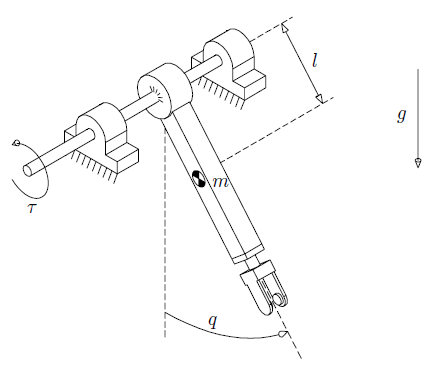
\includegraphics[width=0.6\linewidth]{imagenes/brazo_1gdl.png}
        \caption{Robot manipulador elemental de 1 g.d.l en plano vertical (péndulo rígido actuado)}
        \label{fig:brazo_1gdl}
    \end{figure}

\subsection{Máquina PMSM}
    Para el accionamiento, se utilizará una máquina eléctrica de CA trifásica sincrónica con excitación por imanes permanentes (\textbf{PMSM}) y estator simétrico y equilibrado, con bornes de fases \textit{abc} (coordenadas reales y estacionarias) conectados en configuración estrella (Y) con neutro flotante \textbf{no} accesible.
    \subsubsection{Modelo matemático equivalente del subsistema mecánico}
    Habiendo expresado las ecuaciones para los distintos subsistemas de la máquina PMSM y del tren de transmisión, es posible conjugarlas en un modelo equivalente.
    Sustituyendo \(\omega_l(t)\) de \eqref{eq:cinem_reductor} y \(T_q(t) = rT_d(t)\) de \eqref{eq:torque_reductor} en \eqref{eq:din_pendulo} tenemos:
    \begin{equation}\label{EqAux1}
        \frac{J_l}{r}\frac{d\omega_m(t)}{dt} = rT_d(t)-\frac{b_l}{r}\omega_m(t)-T_l(t)
    \end{equation}
    Despejando \(T_d(t)\) y reemplazando \(T_l(t)\) por \eqref{eq:def_Tl}:
    \begin{equation}\label{Eq1}
        T_d(t)=\frac{J_l}{r^2}\frac{d\omega_m(t)}{dt}+\frac{b_l}{r^2}\omega_m(t)+\frac{1}{r}\left(g\cdot k_l\cdot \sin\Big(\frac{\theta_m(t)}{r}\Big)+T_{ld}(t)\right)
    \end{equation}
    Por otra parte, la ecuación mecánica del rotor del motor es:
    \begin{equation}\label{EqJm}
        J_m\frac{d\omega_m(t)}{dt}=T_m(t)-b_m\omega_m(t)-T_d(t)
    \end{equation}
    Reemplazando \(T_d(t)\) de \eqref{Eq1} en  \eqref{EqJm}:
    \begin{equation}
        J_{eq}\frac{d\omega_m(t)}{dt}=T_m(t)-b_{eq}\omega_m(t)-\frac{1}{r}\Big(g\cdot k_l \sin{\Big(\frac{\theta_m(t)}{r}\Big)} + T_{ld}(t)\Big)
    \end{equation}
    \begin{gather}
        J_{eq} = J_m +\frac{J_l}{r^2}\\
        b_{eq} = b_m + \frac{b_l}{r^2}\\
        \theta_l(t)=\frac{\theta_m(t)}{r}
    \end{gather}
    Podemos entonces, a partir de lo desarrollado, expresar el modelo en el espacio de estados.

    \textbf{Ecuaciones de estado:} Las ecuaciones de estado del subsistema mecánico completo quedan:
    \begin{equation}
        \begin{cases}
            \dot \theta_m(t) = \omega_m(t), \\ 
            \dot\omega_m(t)=-\frac{b_{eq}}{J_{eq}}\omega_m(t)-\frac{g\cdot k_l}{J_{eq}r}\cdot \sin{\Big(\frac{\theta_m(t)}{r}\Big)}+\frac{1}{J_{eq}}T_m(t)-\frac{1}{J_{eq}r}T_{ld}(t),\\
            y(t)=\theta_m(t)
        \end{cases}
        \label{eq: EqEstadoModeloMecanico}
    \end{equation}
    \textbf{Forma matricial}
    \begin{equation}
        \begin{cases}
            \begin{bmatrix}
                \dot\theta_m(t) \\\dot\omega_m(t)
            \end{bmatrix}
            = 
            \begin{bmatrix}
                \omega_m(t)\\
                -\frac{g\cdot k_l}{J_{eq}r}\cdot\sin{\big(\frac{\theta_m(t)}{r}\big)}-\frac{b_{eq}}{J_{eq}}\cdot\omega_m(t)
            \end{bmatrix}
            +
            \begin{bmatrix}
                0 & 0\\
                \frac{1}{J_{eq}} &-\frac{1}{J_{eq}r}
            \end{bmatrix}
            \begin{bmatrix}
                T_m(t)\\
                T_{ld}(t)
            \end{bmatrix}\\
            y(t) = \begin{bmatrix}
                1 & 0
            \end{bmatrix}
            \begin{bmatrix}
                \theta_m(t)\\
                \omega_m(t)
            \end{bmatrix}
        \end{cases}
    \end{equation}
    Nótese cómo se presenta una no linealidad en el primer término, lo que impide formular la matriz $A$ de forma convencional.
    \subsubsection{Modelo del subsistema electromagnético del motor}
    Modelo idealizado equivalente en coordenadas rotóricas \(qd0\), fijas al rotor, obtenido aplicando la \textit{Transformación de Park} al circuito de estator estacionario (marco de referencia virtual eléctrico de rotor, sincrónico solo en régimen estacionario).
    \begin{gather}
        \frac{d\theta_r(t)}{dt} \equiv \omega_r(t) \\
        \theta_r(t)=\int_0^t{\omega_r(\xi)d\xi+\theta_r(0)} \\
        \theta_r(t) \equiv P_p\theta_m(t) \therefore \omega_r(t) = P_p\omega_m(t)
    \end{gather}
    \textbf{Torque electromagnético} = \textit{torque debido a imanes + torque de reluctancia}:
    \begin{equation}
            T_m(t) = \frac{3}{2} P_p \cdot \lambda'^r_m \cdot i^r_{qs}(t) + \frac{3}{2} P_p (L_d-L_q)\cdot i^r_{ds}(t)\cdot i^r_{qs}(t)
            \label{eq:torque_electromagnetico}
    \end{equation}
\textbf{Ecuaciones de tensiones de fase referidas al estator}\\
Dado que es necesario generar un campo magnético rotatorio sinusoidal para efectuar un movimiento en los motores PMSM, y que además los devanados están separados físicamente \(120^\circ\) entre sí, es esperable que el inversor trifásico deba entregar las siguientes tensiones al motor (sistema equilibrado).
\begin{align}
v_{as}(t) &\approx \sqrt{2}\,\frac{V_{sl}(t)}{\sqrt{3}} \cos\big(\theta_{ev}(t)\big) \\
v_{bs}(t) &\approx \sqrt{2}\,\frac{V_{sl}(t)}{\sqrt{3}} \cos\left(\theta_{ev}(t) - \frac{2\pi}{3}\right) \\
v_{cs}(t) &\approx \sqrt{2}\,\frac{V_{sl}(t)}{\sqrt{3}} \cos\left(\theta_{ev}(t) + \frac{2\pi}{3}\right)
\end{align}
Por lo que definiremos:
\[\bm{\mathrm{v}}_{abcs} = (v_{as},\ v_{bs},\ v_{cs})\]

Según la guía de trabajo~\cite{guia_trabajo}, las \textbf{variables manipulables} del inversor son el módulo de la tensión de línea $V_{sl}(t) \in [0;\,48]$~Vca rms y la frecuencia eléctrica $f_e(t) \in [-330;\,+330]$~Hz, cuyo signo define la secuencia de fases ($abc$/$acb$) y, con ello, el sentido de giro del campo rotante. La frecuencia angular eléctrica del estator queda definida por:
\begin{equation}
    \omega_e(t) \equiv 2\pi f_e(t) \equiv \frac{d\theta_{ev}(t)}{dt}
\end{equation}

\textbf{Transformación de Park.} El vínculo entre las variables de fase del estator (coordenadas $abc$, reales y estacionarias) y las coordenadas rotóricas $qd0$ (virtuales, fijas al rotor) se establece mediante la Transformación de Park, en su forma invariante en módulo, aplicable a cualquier variable base $f\in\{v,\,i\}$~\cite{guia_trabajo}. La \textbf{transformación directa} $\big(f_{abcs}(t)\to f_{qd0s}^{r}(t)\big)$ resulta:
\begin{equation}\label{eq:park_directa}
\begin{bmatrix}
f_{qs}^r(t) \\
f_{ds}^r(t) \\
f_{0s}(t)
\end{bmatrix}
= \frac{2}{3}
\begin{bmatrix}
\cos\theta_r(t) & \cos(\theta_r(t)-\frac{2\pi}{3}) & \cos(\theta_r(t)+\frac{2\pi}{3}) \\
\sin\theta_r(t) & \sin(\theta_r(t)-\frac{2\pi}{3}) & \sin(\theta_r(t)+\frac{2\pi}{3}) \\
\frac{1}{2} & \frac{1}{2} & \frac{1}{2}
\end{bmatrix}
\begin{bmatrix}
f_{as}(t) \\
f_{bs}(t) \\
f_{cs}(t)
\end{bmatrix}
\end{equation}
mientras que la \textbf{transformación inversa} $\big(f_{qd0s}^{r}(t)\to f_{abcs}(t)\big)$ es:
\begin{equation}\label{eq:park_inversa}
\begin{bmatrix}
f_{as}(t) \\
f_{bs}(t) \\
f_{cs}(t)
\end{bmatrix}
=
\begin{bmatrix}
\cos\theta_r(t) & \sin\theta_r(t) & 1 \\
\cos(\theta_r(t)-\frac{2\pi}{3}) & \sin(\theta_r(t)-\frac{2\pi}{3}) & 1 \\
\cos(\theta_r(t)+\frac{2\pi}{3}) & \sin(\theta_r(t)+\frac{2\pi}{3}) & 1
\end{bmatrix}
\begin{bmatrix}
f_{qs}^r(t) \\
f_{ds}^r(t) \\
f_{0s}(t)
\end{bmatrix}
\end{equation}
donde $\theta_r(t)=P_p\,\theta_m(t)$ es la posición eléctrica del rotor.

\textbf{Ecuaciones de tensiones de fase referidas al rotor.} Aplicando la transformación directa \eqref{eq:park_directa} al vector de tensiones de fase $\bm{\mathrm{v}}_{abcs}$ se obtienen las tensiones en coordenadas rotóricas $\bm{\mathrm{v}}^{r}_{qd0s}=(v^r_{qs},\,v^r_{ds},\,v_{0s})$, cuyo balance eléctrico es:
    \begin{equation}\label{eq:vqs_rotor}
        v^r_{qs}(t)=R_s(T_s^\circ(t))i^r_{qs}(t) + L_q\frac{d i^r_{qs}(t)}{dt}+[\lambda'^r_m + L_d i^r_{ds}(t)]\omega_r(t)
    \end{equation}
    \begin{equation}\label{eq:vds_rotor}
        v_{ds}^r(t)=R_s(T_s^\circ(t))i^r_{ds}(t)+L_d\frac{d i^r_{ds}(t)}{dt} - L_qi^r_{qs}(t)\omega_r(t)
    \end{equation}
    \begin{equation}\label{eq:v0s_rotor}
        v_{0s}(t)=R_s(T_s^\circ(t))i_{0s}(t)+L_{ls}\frac{d i_{0s}(t)}{dt}
    \end{equation}

    \subsubsection{Modelo del subsistema térmico}
    El calentamiento del estator se modela mediante un circuito térmico concentrado de primer orden, con una capacitancia térmica \(C_{ts}\) asociada al almacenamiento de energía y una resistencia térmica \(R_{ts\text{-}amb}\) asociada a la transferencia de calor hacia el ambiente. La potencia que excita este subsistema proviene de las pérdidas Joule del bobinado estatórico.

    La resistencia del estator depende de la temperatura según:
    \begin{equation}
        R_s\big(T_s^\circ(t)\big)=R_{sREF}\Big[1+\alpha_{Cu}\big(T_s^\circ(t)-T_{sREF}^\circ\big)\Big], \qquad T_{sREF}^\circ=20^\circ\text{C}
    \end{equation}

    Bajo las hipótesis adoptadas, el balance de potencia térmica queda:
    \begin{equation}
        C_{ts}\frac{dT_s^\circ(t)}{dt}=P_{s,perd}(t)-\frac{T_s^\circ(t)-T_{amb}^\circ(t)}{R_{ts\text{-}amb}}
    \end{equation}
    donde
    \begin{equation}
        P_{s,perd}(t)=\frac{3}{2}R_s\big(T_s^\circ(t)\big)\Big(i_{qs}^{r\,2}(t)+i_{ds}^{r\,2}(t)+2i_{0s}^{2}(t)\Big)
    \end{equation}

    Por lo tanto, la ecuación de estado del subsistema térmico es:
    \begin{equation}
        \frac{dT_s^\circ(t)}{dt}=\frac{1}{C_{ts}}\left[\frac{3}{2}R_s\big(T_s^\circ(t)\big)\Big(i_{qs}^{r\,2}(t)+i_{ds}^{r\,2}(t)+2i_{0s}^{2}(t)\Big)-\frac{T_s^\circ(t)-T_{amb}^\circ(t)}{R_{ts\text{-}amb}}\right]
    \end{equation}

    \subsubsection{Modelo no lineal global del accionamiento}
    Una vez definidos el subsistema mecánico equivalente, el subsistema electromagnético en coordenadas \(qd0\) y el subsistema térmico, puede escribirse el modelo no lineal global del accionamiento. Tomando como vector de estado
    \[
        \bm{x}_{NL}(t)=\begin{bmatrix}
            \theta_m(t) & \omega_m(t) & i_{qs}^r(t) & i_{ds}^r(t) & i_{0s}(t) & T_s^\circ(t)
        \end{bmatrix}^T
    \]
    y como entradas
    \[
        \bm{u}_{NL}(t)=\begin{bmatrix}
            v_{qs}^r(t) & v_{ds}^r(t) & v_{0s}(t) & T_{ld}(t) & T_{amb}^\circ(t)
        \end{bmatrix}^T
    \]
    el sistema queda descrito por el siguiente conjunto de ecuaciones de estado no lineales:
    \begin{equation}
    \left\{
        \begin{aligned}
            \dot{\theta}_m(t) &= \omega_m(t) \\[6pt]
            \dot{\omega}_m(t) &= -\frac{b_{eq}}{J_{eq}}\omega_m(t)-\frac{gk_l}{J_{eq}r}\sin\left(\frac{\theta_m(t)}{r}\right)+\frac{1}{J_{eq}}T_m(t)-\frac{1}{J_{eq}r}T_{ld}(t) \\[6pt]
            \dot{i}_{qs}^r(t) &= \frac{1}{L_q}\Big[v_{qs}^r(t)-R_s\big(T_s^\circ(t)\big)i_{qs}^r(t)-\big(\lambda'^r_m+L_d i_{ds}^r(t)\big)\omega_r(t)\Big] \\[6pt]
            \dot{i}_{ds}^r(t) &= \frac{1}{L_d}\Big[v_{ds}^r(t)-R_s\big(T_s^\circ(t)\big)i_{ds}^r(t)+L_q i_{qs}^r(t)\omega_r(t)\Big] \\[6pt]
            \dot{i}_{0s}(t) &= \frac{1}{L_{ls}}\Big[v_{0s}(t)-R_s\big(T_s^\circ(t)\big)i_{0s}(t)\Big] \\[6pt]
            \dot{T}_s^\circ(t) &= \frac{1}{C_{ts}}\left[\frac{3}{2}R_s\big(T_s^\circ(t)\big)\Big(i_{qs}^{r\,2}(t)+i_{ds}^{r\,2}(t)+2i_{0s}^{2}(t)\Big)-\frac{T_s^\circ(t)-T_{amb}^\circ(t)}{R_{ts\text{-}amb}}\right]
        \end{aligned}
    \right.
    \end{equation}
    con
    \begin{equation}
        T_m(t)=\frac{3}{2} P_p \lambda'^r_m i_{qs}^r(t)+\frac{3}{2}P_p(L_d-L_q)i_{ds}^r(t)i_{qs}^r(t),
        \qquad
        \omega_r(t)=P_p\omega_m(t)
    \end{equation}

    Este modelo de 6 estados será la planta de referencia para la implementación en Simulink y para las linealizaciones posteriores. Además, deja explícito que las no linealidades relevantes del sistema provienen del término gravitacional \(\sin(\theta_m/r)\), del acoplamiento electromagnético entre ejes \(q\) y \(d\), y de la dependencia térmica de \(R_s\big(T_s^\circ\big)\).

    % ==========================================================================
    % DEMOSTRACIÓN: La ecuación de secuencia cero no influye con neutro flotante
    % ==========================================================================

    \subsubsection{Irrelevancia de la ecuación de secuencia cero en el modelo del accionamiento}

    La ecuación de secuencia cero del modelo electromagnético en coordenadas rotóricas queda dada por:
    \begin{equation}
        v_{0s}(t)=R_s\!\big(T_s^\circ(t)\big)\,i_{0s}(t)+L_{ls}\frac{d i_{0s}(t)}{dt}
        \label{eq:v0s_rotor_final}
    \end{equation}

    De acuerdo con la consigna, se demostrará que esta ecuación no influye en la dinámica del sistema bajo dos situaciones distintas:

    \begin{enumerate}
        \item sistema trifásico equilibrado con circuito electromagnético de estator simétrico y retorno de neutro;
        \item sistema general no necesariamente simétrico ni equilibrado, pero con centro de estrella flotante (no accesible).
    \end{enumerate}

    % Figura: Conexión estrella con neutro flotante — LCK en nodo n
    \begin{figure}[H]
    \centering
    \begin{circuitikz}[scale=0.95, transform shape, american currents, european resistors]

        % Nodo neutro
        \coordinate (N) at (0,0);
        \filldraw (N) circle (2pt);
        \node[below left=2pt] at (N) {$O$};

        %========================
        % FASE A
        %========================
        \draw
        (N) -- (0,1.2)
        to[L, l=$L_a$, i>^=$i_a$] (0,3.0)
        to[R, l=$R_s$] (0,4.6)
        -- (0,5.2);
        \node[above] at (0,5.2) {$a$};

        % Tensión fase-neutro
        \draw[blue,->,thick] (-1.1,0.15) -- (-1.1,5.05);
        \node[blue,left] at (-1.1,2.6) {$v_{aO}$};

        %========================
        % FASE B
        %========================
        \draw
        (N) -- (-1.15,-0.7)
        to[L, l_=$L_b$, i>_=$i_b$] (-2.8,-1.75)
        to[R, l_=$R_s$] (-4.3,-2.65)
        -- (-4.9,-3.0);
        \node[left] at (-4.9,-3.0) {$b$};

        %========================
        % FASE C
        %========================
        \draw
        (N) -- (1.15,-0.7)
        to[L, l=$L_c$, i>^=$i_c$] (2.8,-1.75)
        to[R, l=$R_s$] (4.3,-2.65)
        -- (4.9,-3.0);
        \node[right] at (4.9,-3.0) {$c$};

        %========================
        % Neutro flotante
        %========================
        \draw[densely dotted, gray, thick] (N) -- (0,-1.3);
        \node[gray, below] at (0,-1.35) {\footnotesize neutro flotante};

    \end{circuitikz}
    \caption{Estator trifásico conectado en estrella con neutro flotante. Al no existir conductor de retorno externo, la Ley de Corrientes de Kirchhoff aplicada en el centro de estrella $O$ impone \(i_a+i_b+i_c=0\), por lo que la componente homopolar de corriente resulta nula: \(i_{0s}(t)\equiv 0\).}
    \label{fig:estrella_neutro_flotante}
    \end{figure}

    \textbf{Definición de la componente homopolar mediante la Transformación de Park.}
    La transformación \(abc \rightarrow qd0\) separa las variables trifásicas en una componente en cuadratura, una componente directa y una componente homopolar. En particular, la componente de secuencia cero de una magnitud genérica \(x\in\{v,i\}\) se define como:
    \begin{equation}
        x_{0s}(t)=\frac{1}{3}\Big(x_a(t)+x_b(t)+x_c(t)\Big)
        \label{eq:def_x0}
    \end{equation}
    Por lo tanto:
    \begin{equation}
        i_{0s}(t)=\frac{1}{3}\Big(i_a(t)+i_b(t)+i_c(t)\Big),
        \qquad
        v_{0s}(t)=\frac{1}{3}\Big(v_a(t)+v_b(t)+v_c(t)\Big)
        \label{eq:def_i0_v0}
    \end{equation}

    \textbf{Caso 1: sistema trifásico equilibrado y estator simétrico, con retorno de neutro.}
    Para un sistema trifásico equilibrado se cumple, en todo instante:
    \begin{equation}
        i_a(t)+i_b(t)+i_c(t)=0
        \label{eq:suma_i_eq}
    \end{equation}
    y, de manera análoga, para tensiones equilibradas:
    \begin{equation}
        v_a(t)+v_b(t)+v_c(t)=0
        \label{eq:suma_v_eq}
    \end{equation}

    Sustituyendo \eqref{eq:suma_i_eq} y \eqref{eq:suma_v_eq} en \eqref{eq:def_i0_v0}, resulta:
    \begin{equation}
        i_{0s}(t)\equiv 0,
        \qquad
        v_{0s}(t)\equiv 0
    \end{equation}

    En consecuencia, la ecuación \eqref{eq:v0s_rotor_final} se reduce a:
    \begin{equation}
        0=R_s\!\big(T_s^\circ(t)\big)\cdot 0 + L_{ls}\frac{d(0)}{dt}
    \end{equation}
    es decir, a una identidad trivial. Por lo tanto, en el caso equilibrado y simétrico, la ecuación de secuencia cero no aporta dinámica al modelo.

    \textbf{Caso 2: sistema general con centro de estrella flotante (no accesible).}
    Considérese ahora el caso general en el que no se supone ni simetría perfecta ni equilibrio de las excitaciones, pero el punto neutro del estator conectado en estrella es flotante, es decir, no existe conductor de retorno desde el centro de estrella hacia una referencia externa.

    \textbf{Demostración mediante Ley de Corrientes de Kirchhoff (LCK).}
    En el centro de estrella \(O\) confluyen únicamente las tres corrientes de fase. Como no existe un cuarto conductor de retorno, la LCK impone:
    \begin{equation}
        i_a(t)+i_b(t)+i_c(t)=0
        \label{eq:LCK_neutro_flotante}
    \end{equation}

    Esta restricción es puramente topológica y no depende de que el sistema sea o no equilibrado. Por lo tanto, usando nuevamente la definición \eqref{eq:def_i0_v0}:
    \begin{equation}
        i_{0s}(t)=\frac{1}{3}\Big(i_a(t)+i_b(t)+i_c(t)\Big)=0
    \end{equation}
    o sea,
    \begin{equation}
        \boxed{i_{0s}(t)\equiv 0}
        \label{eq:i0_neutro_flotante}
    \end{equation}

    \textbf{Interpretación mediante la Transformación de Park:}
    La componente homopolar obtenida por Park representa la parte común a las tres fases. Si la suma instantánea de corrientes de fase es nula, entonces la proyección sobre el eje \(0\) también es nula. Es decir, el subespacio homopolar no queda excitado:
    \begin{equation}
        i_{0s}(t)\equiv 0
    \end{equation}

    Sustituyendo este resultado en \eqref{eq:v0s_rotor_final}, se obtiene:
    \begin{equation}
        v_{0s}(t)=R_s\!\big(T_s^\circ(t)\big)\cdot 0 + L_{ls}\frac{d(0)}{dt}=0
    \end{equation}
    de modo que la ecuación de secuencia cero vuelve a quedar satisfecha de forma trivial, sin aportar dinámica propia al sistema.

    En consecuencia, la componente homopolar no aporta dinámica relevante para el análisis electromecánico del accionamiento bajo las hipótesis adoptadas. Este resultado justifica que, en los desarrollos posteriores, el eje \(0\) pueda omitirse cuando se trabaje con el modelo reducido en coordenadas \(qd\).

% ==========================================================================
% SECCIÓN II-E: VALIDACIÓN POR SIMULACIÓN (LAZO ABIERTO)
% ==========================================================================

\subsection{Implementación y Validación en Entorno de Simulación}
Se implementó el modelo matemático completo en el entorno MATLAB/Simulink, estructurando el sistema mediante bloques funcionales interconectados que representan las ecuaciones diferenciales deducidas previamente.

La arquitectura de la simulación se diseñó para validar tanto la dinámica de la planta como la coherencia de las transformaciones de coordenadas. El flujo de señales se configura de la siguiente manera:
\begin{enumerate}
    \item \textbf{Generación de Consigna:} Se establecen tensiones de referencia constantes en el marco rotórico ($v_{qs}^{r*}=5$~V, $v_{ds}^{r*}=0$).
    \item \textbf{Transformaciones de Coordenadas:} Las tensiones $dq$ se convierten al marco trifásico $abc$ mediante la \textit{Transformación Inversa de Park} y se reconvierten inmediatamente al marco $dq$ mediante la \textit{Transformación de Park}. Esta estructura en bucle ("Back-to-Back") permite verificar la integridad matemática de los algoritmos antes de ingresar a la planta.
    \item \textbf{Planta Física:} Las señales resultantes alimentan al \textbf{Subsistema Electromecánico} y al \textbf{Subsistema Mecánico}, interactuando simultáneamente con el \textbf{Subsistema Térmico}.
\end{enumerate}

% FIGURA DIAGRAMA SIMULINK
\begin{figure}[H]
    \centering
    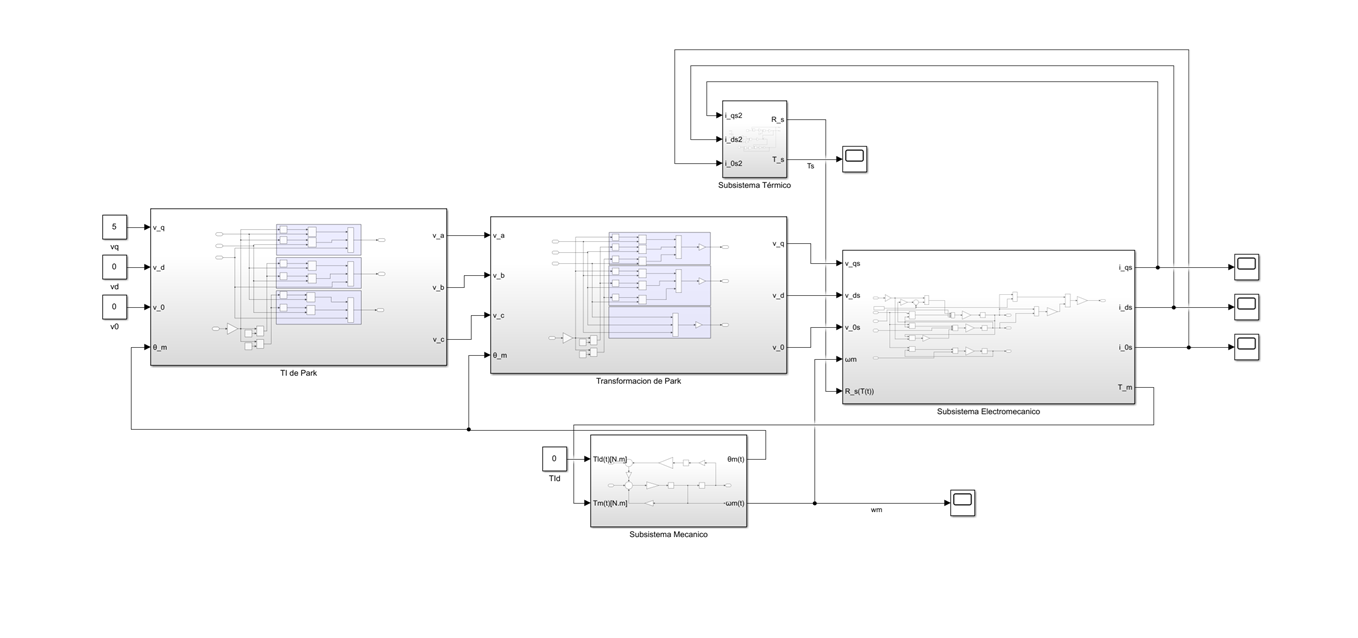
\includegraphics[width=1.0\linewidth]{imagenes/simulink_diagrama_completo.png}
    \caption{Diagrama de bloques implementado en Simulink. Se destaca la estructura de validación con Transformaciones directa e inversa y la interconexión de los subsistemas.}
    \label{fig:simulink_top}
\end{figure}

\subsubsection{Resultados del Ensayo a Lazo Abierto}
Se realizó un ensayo de excitación al escalón con $v_{qs}^{r*}=5$~V y carga nula ($T_{ld}=0$), partiendo de condiciones iniciales de reposo y equilibrio térmico ($T_s^\circ(0)=20^\circ$C).

\textbf{Análisis Electromecánico:}
La Fig. \ref{fig:res_elec_mec} vincula la dinámica eléctrica con la mecánica:
\begin{itemize}
    \item \textbf{Superior ($i_{qs}^r$):} Al aplicar la tensión, la corriente aumenta rápidamente ($\tau_e = L_q/R_s$). Sin embargo, a medida que el motor gana velocidad, la aparición de la fuerza contraelectromotriz ($e = \lambda'^r_m \omega_r$) se opone a la tensión aplicada, provocando la reducción de la corriente observada a partir de $t \approx 0{,}1$ s.
    \item \textbf{Inferior ($\omega_m$):} El torque generado por la corriente acelera el rotor venciendo la inercia $J_{eq}$. La velocidad se estabiliza cuando el torque motor se iguala con el torque de fricción viscosa.
\end{itemize}

% FIGURA COMBINADA CORRIENTE/VELOCIDAD (CLAVADA AQUÍ CON [H])
\begin{figure}[H]
    \centering
    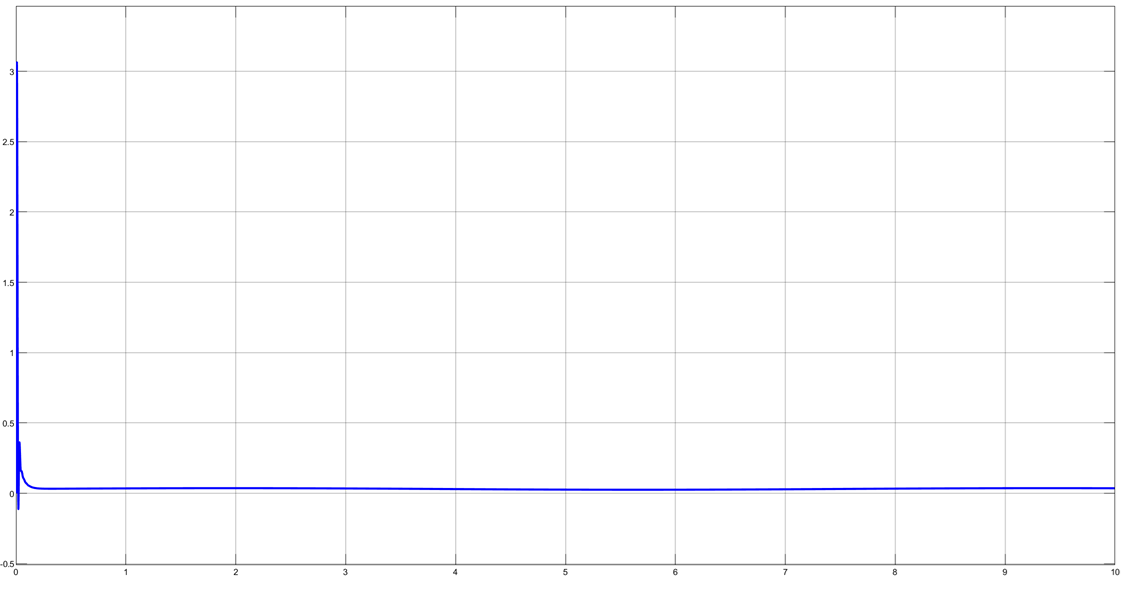
\includegraphics[width=0.9\linewidth]{imagenes/resultado_corriente.png} \\[0.1cm]
    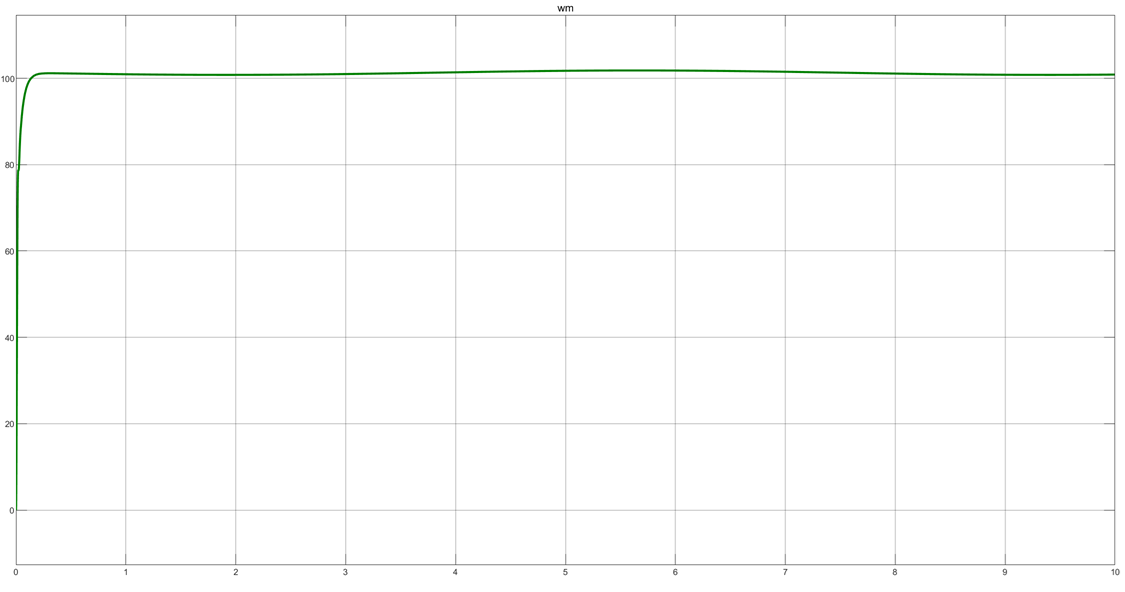
\includegraphics[width=0.9\linewidth]{imagenes/resultado_velocidad.png}
    \caption{Respuesta dinámica al escalón de tensión $v_{qs}^{r*}=5$~V. \textbf{Arriba:} Corriente de estator $i_{qs}^r$ [A], mostrando el transitorio inductivo y el efecto de la fuerza contraelectromotriz. \textbf{Abajo:} Velocidad mecánica del rotor $\omega_m$ [rad/s].}
    \label{fig:res_elec_mec}
\end{figure}

\textbf{Análisis Térmico:}
La Fig. \ref{fig:res_term} muestra la evolución de la temperatura del estator. Se observa un inicio correcto en $T_{amb}^\circ=20^\circ$C.
Es notable que la pendiente de calentamiento no es constante: es máxima al inicio (cuando la corriente es alta y el rotor está detenido) y disminuye cuando el motor acelera y la corriente baja debido a la fuerza contraelectromotriz. Este comportamiento valida el correcto acoplamiento entre las variables eléctricas ($i^2 R$) y la dinámica mecánica en el modelo térmico.

% FIGURA TÉRMICA (CLAVADA AQUÍ CON [H])
\begin{figure}[H]
    \centering
    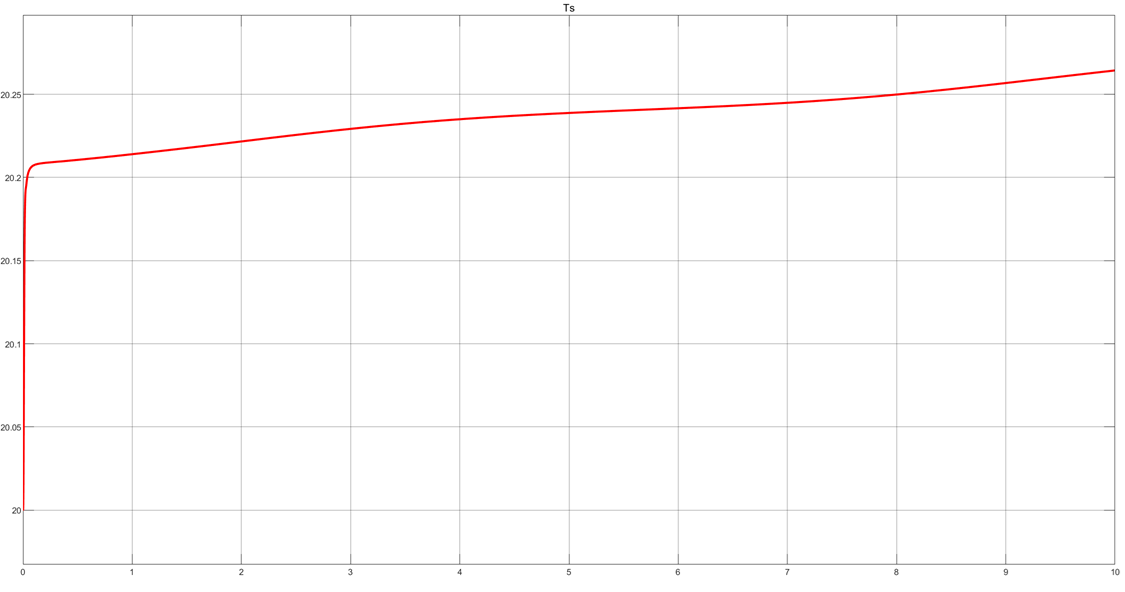
\includegraphics[width=0.9\linewidth]{imagenes/resultado_temperatura.png}
    \caption{Evolución de la temperatura del estator $T_s^\circ(t)$. Nótese el cambio de pendiente provocado por la variación de la corriente durante el arranque.}
    \label{fig:res_term}
\end{figure}

% ESTE COMANDO ASEGURA QUE LAS FOTOS TERMINEN AQUÍ Y NO PASEN A LA MATEMÁTICA
\clearpage



%-------------- LPV -----------------
\subsection{Linealización mediante el método de \textit{pequeñas señales}: Modelo LPV con \(i^r_{ds}\neq 0\)}
A partir del modelo NL anteriormente presentado, es posible obtener, a través de la linealización jacobiana mediante aproximación con serie de Taylor truncada de primer orden en un punto genérico de operación, un modelo lineal más simple de analizar y controlar.

Considerando que el modelo actual es de la forma \[\bm{\dot x} =\bm{f}(\bm{x},\bm{u})\]
donde primero se deben encontrar los puntos de equilibrio del sistema, es decir, los valores \(\bm{x}_o\) y \(\bm{u}_o\) tales que \(\bm{\dot x}_o = \bm{f}(\bm{x}_o,\bm{u}_o)\). Definiendo \(\bm{x}=\bm{x}_o+\Delta\bm{x}\) y \(\bm{u}=\bm{u}_o+\Delta\bm{u}\), se expande la ecuación no lineal en términos de las perturbaciones respecto a estos valores de equilibrio, lo que resulta en:
\begin{equation*}
    \bm{\dot x}_o + \Delta\bm{\dot x} \cong \bm{f}(\bm{x}_o,\bm{u}_o) + \bm{A}_o\Delta\bm{x}+\bm{B}_o\Delta\bm{u}
\end{equation*}
donde \(\bm{A}_o\) y \(\bm{B}_o\) son la mejor aproximación lineal de la función \(\bm{f}(\bm{x},\bm{u})\) en \(\bm{x}_o,\bm{u}_o\), calculándose:
\begin{equation*}
    \bm{A}_o = \left[ \frac{\partial \bm{f}}{\partial \bm{x}} \right]_{\bm{x}_o,\bm{u}_o} \quad \text{y} \quad \bm{B}_o = \left[ \frac{\partial \bm{f}}{\partial \bm{u}} \right]_{\bm{x}_o,\bm{u}_o}
\end{equation*}
Restando la solución de equilibrio y dejando la ecuación solo en variables incrementales nos queda:
\begin{equation*}
    \Delta\bm{\dot x}=\bm{A}_o\Delta\bm{x}+\bm{B}_o\Delta\bm{u}
\end{equation*}
Es decir, una ecuación diferencial lineal alrededor del punto de equilibrio cuasi-estático.
\subsubsection{Implementación en caso genérico de operación, \(\omega_{m,o}(t)=\mathrm{cte}\)}
Utilizando entonces las ecuaciones vistas podemos comenzar a linealizar nuestro sistema mediante el método de pequeñas señales.
Primero, se encuentra el espacio de operación global no lineal, que es el espacio donde se resolverá la primera parte de la ecuación expandida, $\bm{f}(\bm{x}_o,\bm{u}_o)=0$.

\begin{equation}
\left\{
    \begin{aligned}
        \frac{d\theta_{m,o}(t)}{dt} &= \omega_{m,o}(t) = \text{cte} \\[10pt]
        %
        \frac{d\omega_{m,o}(t)}{dt} &= \frac{1}{J_{eq}} \left[ -b_{eq}\omega_{m,o}(t) + \frac{3}{2}P_p \left[ \lambda'^r_m + (L_d - L_q)i^r_{ds,o}(t) \right] i^r_{qs,o}(t) \right. \\
        &\quad \left. - g \cdot k_l \sin\left(\frac{\theta_{m,o}(t)}{r}\right) - \frac{1}{r}T_{ld,o}(t) \right] = 0 \\[10pt]
        %
        \frac{di^r_{qs,o}(t)}{dt} &= \frac{1}{L_q} \left[ v^r_{qs,o}(t) - R_s(T_{s,o}^\circ(t))i^r_{qs,o}(t) - (\lambda'^r_m + L_d i^r_{ds,o}(t))P_p \omega_{m,o}(t) \right] = 0 \\[10pt]
        %
        \frac{di^r_{ds,o}(t)}{dt} &= \frac{1}{L_d} \left[ v^r_{ds,o}(t) - R_s(T_{s,o}^\circ(t))i^r_{ds,o}(t) + L_q i^r_{qs,o}(t)P_p \omega_{m,o}(t) \right] = 0 \\[10pt]
        %
        \frac{di_{0s,o}(t)}{dt} &= \frac{1}{L_{ls}} \left( v_{0s,o}(t) - R_s(T_{s,o}^\circ(t))i_{0s,o}(t) \right) = 0 \\[10pt]
        %
        \frac{dT_{s,o}^\circ(t)}{dt} &= \frac{1}{C_{ts}} \left[ \frac{3}{2}R_s(T_{s,o}^\circ(t)) \left( i^r_{qs,o}(t)^2 + i^r_{ds,o}(t)^2 + 2i_{0s,o}(t)^2 \right) \right. \\
        &\quad \left. - \frac{1}{R_{ts\text{-}amb}} (T_{s,o}^\circ(t) - T_{amb,o}^\circ(t)) \right] = 0
    \end{aligned}
\right.
\end{equation}
Luego la parte lineal dinámica, que es de principal interés en este análisis.
\begin{equation*}
    \Delta\bm{\dot x}(t) = \underbrace{\left. \frac{\partial \bm f}{\partial \bm x} \right|_o}_{\bm A_o}\Delta\bm x(t) + \underbrace{\left. \frac{\partial \bm f}{\partial \bm u} \right|_o}_{\bm B_o}\Delta\bm u(t); \quad \Delta\bm x(0) = 0
\end{equation*}
\begin{equation*}
\left\{
    \begin{aligned}
        \Delta \dot{\theta}_m(t) &= \Delta \omega_m(t) \\[10pt]
        %
        \Delta \dot{\omega}_m(t) &= \frac{1}{J_{eq}} \left[ \frac{3}{2} P_p \left\{ [\lambda'^r_m + (L_d - L_q) \cdot i^r_{ds,o}] \cdot \Delta i_{qs}^r(t) + (L_d - L_q) \cdot i^r_{qs,o} \cdot \Delta i_{ds}^r(t) \right\} - b_{eq} \cdot \Delta \omega_m(t) \right. \\
        &\quad \left. - \frac{g \cdot k_l}{r^2} \cdot \cos\left(\frac{\theta_{m,o}}{r}\right) \cdot \Delta \theta_m(t) - \frac{\Delta T_{ld}(t)}{r} \right] \\[10pt]
        %
        \Delta \dot{i}_{qs}^r(t) &= \frac{1}{L_q} \left[ \Delta v_{qs}^r(t) - R_{s,o} \cdot \Delta i_{qs}^r(t) - R_{sREF} \alpha_{Cu} \Delta T_s^\circ(t) \cdot i^r_{qs,o} - \{\lambda'^r_m + L_d \cdot i^r_{ds,o}\} P_p \cdot \Delta \omega_m(t) \right. \\
        &\quad \left. - L_d P_p \omega_{m,o} \cdot \Delta i_{ds}^r(t) \right] \\[10pt]
        %
        \Delta \dot{i}_{ds}^r(t) &= \frac{1}{L_d} \left[ \Delta v_{ds}^r(t) - R_{s,o} \cdot \Delta i_{ds}^r(t) - R_{sREF} \alpha_{Cu} \Delta T_s^\circ(t) \cdot i^r_{ds,o} + L_q \cdot i^r_{qs,o} \cdot P_p \cdot \Delta \omega_m(t) \right. \\
        &\quad \left. + L_q \cdot P_p \cdot \omega_{m,o} \cdot \Delta i_{qs}^r(t) \right] \\[10pt]
        %
        \Delta \dot{i}_{0s}(t) &= \frac{1}{L_{ls}} \left[ \Delta v_{0s}(t) - R_{s,o} \cdot \Delta i_{0s}(t) - R_{sREF} \alpha_{Cu} \Delta T_s^\circ(t) \cdot i_{0s,o} \right] \\[10pt]
        %
        \Delta \dot{T}_s^\circ(t) &= \frac{1}{C_{ts}} \left[ \frac{3}{2} \cdot R_{s,o} \cdot (2 \cdot i^r_{qs,o} \cdot \Delta i_{qs}^r(t) + 2 \cdot i^r_{ds,o} \cdot \Delta i_{ds}^r(t) + 4 \cdot i_{0s,o} \cdot \Delta i_{0s}(t)) \right. \\
        &\quad + \frac{3 \alpha_{Cu} R_{sREF}}{2} (i^r_{qs,o}(t)^2 + i^r_{ds,o}(t)^2 + 2i_{0s,o}(t)^2) \cdot \Delta T_s^\circ(t) \\
        &\quad \left. - \frac{1}{R_{ts\text{-}amb}} (\Delta T_s^\circ(t) - \Delta T_{amb}^\circ(t)) \right]
    \end{aligned}
\right.
\end{equation*}
donde \(R_{s,o}=R_s(T_{s,o}^\circ)\).
\begin{equation*}
\bm{A}_o = \begin{bmatrix}
0 & 1 & 0 & 0 & 0 & 0 \\
-\frac{g k_l \cos\left(\frac{\theta_{m,o}}{r}\right)}{J_{eq} r^2} & -\frac{b_{eq}}{J_{eq}} & \frac{3 P_p (\lambda'^r_m + i^r_{ds,o} (L_d - L_q))}{2 J_{eq}} & \frac{3 P_p i^r_{qs,o} (L_d - L_q)}{2 J_{eq}} & 0 & 0 \\
0 & -\frac{P_p (\lambda'^r_m + L_d i^r_{ds,o})}{L_q} & -\frac{R_{s,o}}{L_q} & -\frac{L_d P_p \omega_{m,o}}{L_q} & 0 & -\frac{R_{sREF} \alpha_{Cu} i^r_{qs,o}}{L_q} \\
0 & \frac{L_q P_p i^r_{qs,o}}{L_d} & \frac{L_q P_p \omega_{m,o}}{L_d} & -\frac{R_{s,o}}{L_d} & 0 & -\frac{R_{sREF} \alpha_{Cu} i^r_{ds,o}}{L_d} \\
0 & 0 & 0 & 0 & -\frac{R_{s,o}}{L_{ls}} & -\frac{R_{sREF} \alpha_{Cu} i_{0s,o}}{L_{ls}} \\
0 & 0 & \frac{3 R_{s,o} i^r_{qs,o}}{C_{ts}} & \frac{3 R_{s,o} i^r_{ds,o}}{C_{ts}} & \frac{6 R_{s,o} i_{0s,o}}{C_{ts}} & \Gamma_{th,o}
\end{bmatrix}
\end{equation*}

donde la constante de disipación térmica acoplada $\Gamma_{th,o}$ se define como:
\begin{equation*}
\Gamma_{th,o} = -\frac{\frac{1}{R_{ts\text{-}amb}} - \frac{3 R_{sREF} \alpha_{Cu} (2 i_{0s,o}^2 + i^{r\,2}_{ds,o} + i^{r\,2}_{qs,o})}{2}}{C_{ts}}
\end{equation*}
Las matrices de entrada manipulada y de perturbación quedan respectivamente:
\begin{equation*}
\bm B_o^c = \begin{bmatrix}
0 & 0 & 0 \\
0 & 0 & 0 \\
\frac{1}{L_q} & 0 & 0 \\
0 & \frac{1}{L_d} & 0 \\
0 & 0 & \frac{1}{L_{ls}} \\
0 & 0 & 0
\end{bmatrix},
\end{equation*}

\begin{equation*}
\bm B_o^d = \begin{bmatrix}
0 & 0 \\
-\frac{1}{J_{eq} r} & 0 \\
0 & 0 \\
0 & 0 \\
0 & 0 \\
0 & \frac{1}{C_{ts} R_{ts\text{-}amb}}
\end{bmatrix} 
\end{equation*}
El modelo global LPV toma la forma:
\begin{equation}
\begin{bmatrix}
\Delta \dot{\theta}_m(t) \\
\Delta \dot{\omega}_m(t) \\
\Delta \dot{i}_{qs}^r(t) \\
\Delta \dot{i}_{ds}^r(t) \\
\Delta \dot{i}_{0s}(t) \\
\Delta \dot{T}_s^\circ(t)
\end{bmatrix} = \bm A_o \cdot
\begin{bmatrix}
\Delta \theta_m(t) \\
\Delta \omega_m(t) \\
\Delta i_{qs}^r(t) \\
\Delta i_{ds}^r(t) \\
\Delta i_{0s}(t) \\
\Delta T_s^\circ(t)
\end{bmatrix} + \bm B_o^c \cdot
\begin{bmatrix}
\Delta v_{qs}^r(t) \\
\Delta v_{ds}^r(t) \\
\Delta v_{0s}(t)
\end{bmatrix} + \bm B_o^d \cdot
\begin{bmatrix}
\Delta T_{ld}(t) \\
\Delta T_{amb}^\circ(t)
\end{bmatrix}.
\end{equation}


\subsection{Linealización por Retroalimentación NL: Modelo LTI equivalente}
El objetivo de esta sección es obtener un modelo lineal invariante en el tiempo (LTI) a partir de la planta no lineal, aplicando estrategias de control vectorial con campo orientado. Para lograr esto, se imponen restricciones matemáticas en las entradas manipuladas mediante retroalimentación de estado, buscando desacoplar los canales de flujo magnético y torque. Para el modelo LTI, se asume la dinámica térmica como lineal, con $R_s = R_{s0} = 1{,}058\ \Omega$ constante, evaluada a la temperatura media de operación del estator ($\approx 29{,}5\,^\circ$C) y no al valor de referencia $R_{sREF} = 1{,}02\ \Omega$ a $20\,^\circ$C. Además, el torque de carga total $T_l(t)$ ---definido en el modelo mecánico--- se considera una \textbf{entrada de perturbación externa (exógena)} del modelo, aplicada directamente sobre la dinámica mecánica. De esta forma, la matriz de estado $\bm{A}$ resulta lineal e invariante en el tiempo.

\subsubsection{Restricción o ley de control mínima en el eje $d$}
Para lograr el desacoplamiento de flujo y torque, se impone el requisito de mantener la corriente del eje directo nula: $i_{ds}^r(t) \equiv 0$. Analizando la ecuación diferencial de dicho estado:
\begin{equation}
    \frac{di_{ds}^r(t)}{dt} = \frac{1}{L_d} \left[ v_{ds}^r(t) - R_{s0} i_{ds}^r(t) + L_q i_{qs}^r(t) \omega_r(t) \right]
\end{equation}

La \textbf{ley de control mínima} requerida sobre la variable manipulada virtual $v_{ds}^r(t)$ para cancelar la fuerza contraelectromotriz cruzada y forzar la dinámica a cero (asumiendo la hipótesis de que el estado inicial es nulo, $i_{ds}^r(0) = 0$) es:
\begin{equation} \label{eq:vds_minima}
    v_{ds}^r(t) = -L_q \cdot i_{qs}^r(t) \cdot \omega_r(t)
\end{equation}

Al aplicar este voltaje, la dinámica del eje directo se anula y la ecuación de torque electromagnético se vuelve lineal y proporcional a $i_{qs}^r$.

\subsubsection{Ecuaciones escalares y matriciales del modelo LTI nominal}
Aplicando las leyes de control obtenidas \eqref{eq:vds_minima} y \eqref{eq:vqs_comp}, y asumiendo $i_{ds}^r(t) \equiv 0$, el sistema electromecánico global se reduce a un modelo LTI equivalente. El sistema de ecuaciones diferenciales resultante es:
\begin{equation} \label{eq:sis_escalar_LTI}
\begin{cases}
    \vspace{0.2cm}
    \dfrac{d\theta_m(t)}{dt} = \omega_m(t) \\
    \vspace{0.2cm}
    \dfrac{d\omega_m(t)}{dt} = \dfrac{1}{J_{eq}}\Big[\frac{3 P_p \lambda'^r_m}{2} i_{qs}^r(t) - b_{eq} \omega_m(t) - \frac{1}{r} T_l(t)\Big] \\
    \dfrac{di_{qs}^r(t)}{dt} = \dfrac{1}{L_q}\Big[-P_p \lambda'^r_m \omega_m(t) - R_{s0}\cdot i_{qs}^r(t) + v_{qs}(t)\Big]
\end{cases}
\end{equation}
Aunque se desprecie el efecto del subsistema térmico en la dinámica del modelo LTI, es interesante seguir estudiando la temperatura del estator en la simulación, por lo que también se considera la siguiente ecuación
\[\dfrac{dT_s^\circ(t)}{dt} = \dfrac{1}{C_{ts}}\Big[\frac{3}{2}R_{s0}\cdot i_{qs}^{r\,2}(t)-\frac{1}{R_{ts\text{-}amb}}\big(T_s^\circ(t) - T_{amb}^\circ(t)\big)\Big]\]
Definiendo el vector de estados nominal $\bm{x}_{LTI} = [\theta_m, \omega_m, i_{qs}^r]^T$, la representación matricial de estado resulta:

\begingroup
\renewcommand{\arraystretch}{1.8} 
\begin{equation}
\begin{bmatrix}
\dot{\theta}_m (t)\\
\dot{\omega}_m(t)\\
\dot{i}_{qs}^r(t)
\end{bmatrix}
= 
\underbrace{
\begin{bmatrix}
0 & 1 & 0 \\
0  & -\frac{b_{eq}}{J_{eq}} & \frac{3 P_p \lambda'^r_m}{2 J_{eq}}     \\
 0 &  -\frac{P_p \lambda'^r_m}{L_q} & -\frac{R_{s0}}{L_q}
\end{bmatrix}
}_{\bm{A}}
\begin{bmatrix}
\theta_m(t) \\
\omega_m (t)\\
i_{qs}^r(t) 
\end{bmatrix}
+
\underbrace{
\begin{bmatrix}
0  \\
0  \\
\frac{1}{L_q} 
\end{bmatrix}
}_{\bm{B_c}}
v_{qs}(t) 
+
\underbrace{
\begin{bmatrix}
0 \\
-\frac{1}{rJ_{eq}} \\
0
\end{bmatrix}
}_{\bm{B_d}}
T_l(t)
\end{equation}\normalsize
\endgroup

La ecuación de salida, midiendo la posición, es:
\begin{equation}
\bm{y}(t) = \theta_m(t) = 
\underbrace{
\begin{bmatrix} 1 & 0 & 0 \end{bmatrix}
}_{\bm{C}_{LTI}} \bm{x}_{LTI} 
+ 
\underbrace{
\begin{bmatrix} 0 & 0 \end{bmatrix}
}_{\bm{D}_{LTI}} \bm{u}_{LTI}
\end{equation}



% Aquí insertas la imagen de tu diagrama de bloques del sistema LTI.
\begin{figure}[H]
    \centering
    
\includegraphics[width=\textwidth]{imagenes/LTI equivalente_nominal.png}
    \caption{Diagrama de bloques de estado del modelo LTI equivalente nominal.}
    \label{fig:diagrama_LTI}
\end{figure}


\subsubsection{Dinámica residual equivalente y modelo LTI aumentado}
El modelo nominal desarrollado asume $i_{ds}^r(0) = 0$. En el caso general donde no se cumple esta hipótesis ($i_{ds}^r(0) \neq 0$), la inyección de la ley de control mínima \eqref{eq:vds_minima} en la ecuación del eje directo reduce la misma a una EDO autónoma de primer orden:
\begin{equation}
    \frac{di_{ds}^r(t)}{dt} = -\frac{R_{s0}}{L_d} i_{ds}^r(t) \implies i_{ds}^r(t) = i_{ds}^r(0) e^{-\frac{R_{s0}}{L_d} t}
\end{equation}

Esto demuestra una \textbf{dinámica residual} donde la corriente decae exponencialmente hacia cero. Como el acoplamiento cruzado en el eje $q$ ya fue cancelado matemáticamente por la ley \eqref{eq:vqs_comp}, esta dinámica transitoria ocurre de forma totalmente independiente del resto de los estados. 
Aun así, esta volvería a acoplar temporalmente la corriente en eje directo con la velocidad, ya que:
\begin{equation*}
    v_{qs}^r(t) = L_q \dfrac{di_{qs}^r(t)}{dt} + R_s(t)i_{qs}^r(t)+\lambda'^r_m\omega_r(t)+  \underbrace{P_pL_di_{ds}^r(t)\omega_m(t)}_{\text{Acoplamiento}}
\end{equation*}
Para representar el sistema completo, se incorpora esta EDO al modelo LTI, definiendo el vector de estado aumentado $\bm{x}_{aug} = [\theta_m, \omega_m, i_{qs}^r, i_{ds}^r]^T$. 

\subsubsection{Ley de control complementaria en el eje $q$}
Si consideramos la dinámica residual analizada en el punto anterior, se puede ver que se producirá acoplamiento cruzado no lineal temporal en el eje de cuadratura debido al término $\omega_r L_d i_{ds}^r$. 

Para eliminar completamente esta dependencia y hacer que el eje $q$ sea lineal, se inyecta una compensación dinámica o \textbf{ley de control complementaria}. La tensión virtual comandada será:
\begin{equation} \label{eq:vqs_comp}
    v_{qs}^{r*}(t) = v_{qs}(t) + \underbrace{\omega_r(t) L_d i_{ds}^r(t)}_{\text{Cancelación cruzada}}
\end{equation}
donde $v_{qs}(t)$ pasa a ser la nueva entrada de control lineal del sistema.

El \textbf{modelo LTI aumentado} de cuarto orden resultante es:
\begin{equation} \label{eq:sis_escalar_LTI_aug}
\begin{cases}
    \vspace{0.2cm}
    \dfrac{d\theta_m(t)}{dt} = \omega_m(t) \\
    \vspace{0.2cm}
    \dfrac{d\omega_m(t)}{dt} = \dfrac{1}{J_{eq}}\Big[\frac{3 P_p \lambda'^r_m}{2} i_{qs}^r(t) - b_{eq} \omega_m(t) - \frac{1}{r} T_l(t)\Big] \\
    \dfrac{di_{qs}^r(t)}{dt} = \dfrac{1}{L_q}\Big[-P_p \lambda'^r_m \omega_m(t) - R_{s0}\cdot i_{qs}^r(t) + v_{qs}(t)\Big] \\
    \dfrac{di_{ds}^r(t)}{dt} = \dfrac{-R_{s0}}{L_d}i_{ds}^r(t)
\end{cases}
\end{equation}
Al igual que en el modelo nominal, la temperatura del estator se sigue simulando aparte mediante su ecuación no lineal, sin formar parte de la dinámica LTI de cuarto orden:
\[\dfrac{dT_s^\circ(t)}{dt} = \dfrac{1}{C_{ts}}\Big[\frac{3}{2}R_{s0}\cdot \big(i_{qs}^{r\,2}(t)+i_{ds}^{r\,2}(t)\big)-\frac{1}{R_{ts\text{-}amb}}\big(T_s^\circ(t) - T_{amb}^\circ(t)\big)\Big]\]
\begingroup
\renewcommand{\arraystretch}{1.8} 
\footnotesize\begin{equation}
\begin{bmatrix}
\dot{\theta}_m (t)\\
\dot{\omega}_m(t)\\
\dot{i}_{qs}^r(t)\\
\dot{i}_{ds}^r(t)
\end{bmatrix}
= 
\begin{bmatrix}
0 & 1 & 0 & 0 \\
0  & -\frac{b_{eq}}{J_{eq}} & \frac{3 P_p \lambda'^r_m}{2 J_{eq}} & 0 \\
 0 &  -\frac{P_p \lambda'^r_m}{L_q} & -\frac{R_{s0}}{L_q} & 0 \\
 0 & 0 & 0 & -\frac{R_{s0}}{L_d}
\end{bmatrix}
\begin{bmatrix}
\theta_m(t) \\
\omega_m (t)\\
i_{qs}^r(t) \\
i_{ds}^r(t)
\end{bmatrix}
+
\begin{bmatrix}
0  \\
0  \\
\frac{1}{L_q} \\
0
\end{bmatrix}
v_{qs}(t) 
+
\begin{bmatrix}
0 \\
-\frac{1}{rJ_{eq}} \\
0 \\
0
\end{bmatrix}
T_l(t)
\end{equation}\normalsize
\endgroup
\subsubsection{Diagrama de bloques de estado (forma desagregada)}
A partir de las ecuaciones matriciales, se construye el diagrama de bloques del sistema linealizado equivalente.
\begin{figure}[H]
    \centering
    
\includegraphics[width=\textwidth]{imagenes/LTI equivalente_aumentado.png}
    \caption{Diagrama de bloques de estado del modelo LTI equivalente aumentado.}
    \label{fig:diagrama_LTI_aumentado}
\end{figure}
\subsubsection{Implementación en el modelo global NL}
La implementación física de esta Linealización por Retroalimentación requiere un \textit{controlador parcial} acoplado a la planta NL original. 
\begin{enumerate}
    \item Recibe la acción de control lineal generada por un controlador de movimiento ($v_{qs}$).
    \item Calcula los voltajes de desacoplamiento interno en tiempo real utilizando las lecturas de los sensores idealizados ($\bm{i}_{abcs} \rightarrow \bm{i}_{qd0s}^r$ y $\omega_m$), aplicando las Ecuaciones \eqref{eq:vds_minima} y \eqref{eq:vqs_comp}.
    \item Estas señales resultantes ($v_{qs}^{r*}$ y $v_{ds}^{r*}$) pasan por un bloque de Transformación de Park Inversa ($\theta_r = P_p \theta_m$).
    \item Finalmente, se envían los voltajes calculados $\bm{v}_{abcs}^*$ al inversor, el cual excita físicamente la planta NL.
\end{enumerate}
\begin{figure}[H]
    \centering
    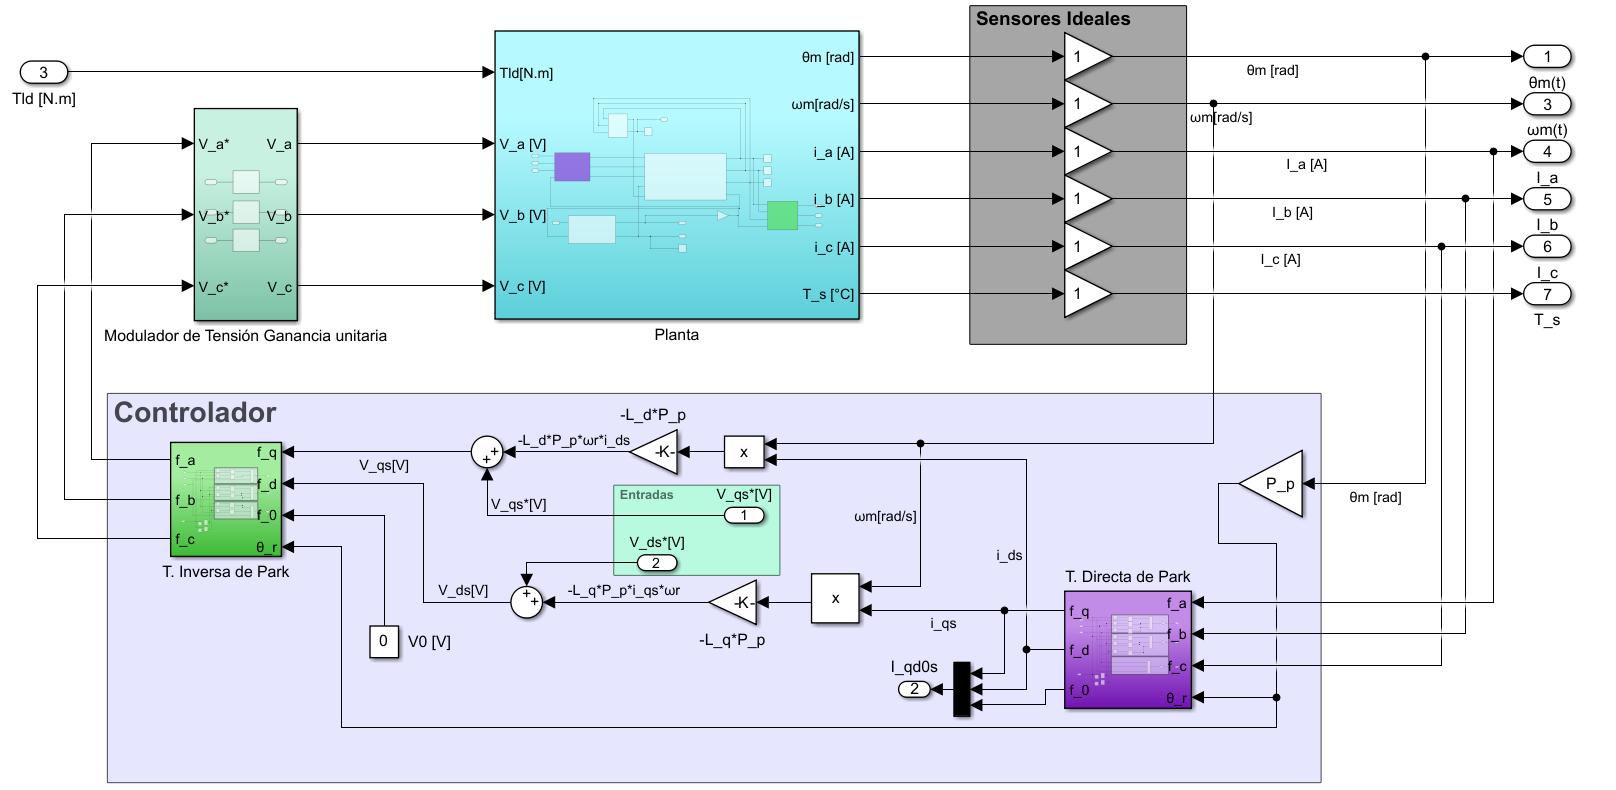
\includegraphics[width=\textwidth]{imagenes/NL con realimentacion NL.png}
    \caption{Diagrama de bloques de implementación de la realimentación sobre la planta no lineal.}
    \label{fig:diagrama_realimentacion_nl}
\end{figure}
\subsection{Comparación del modelo LPV con el modelo LTI aumentado}
\subsubsection{Comparación: LTI Aumentado vs. LPV con \(I^r_{ds,o} \equiv 0\)}

Si bien ambos modelos buscan representar la dinámica del sistema mediante ecuaciones de estado lineales, difieren en su desarrollo y en cómo manejan las restricciones del sistema físico. Las principales diferencias y similitudes se detallan a continuación:

\begin{enumerate}
    \item \textbf{Naturaleza de la linealización:}
    \begin{itemize}
        \item \textit{Modelo LPV:} Se obtiene mediante una expansión en Series de Taylor truncada a primer orden. Es una aproximación de ``pequeña señal'' \cite{franklin_feedback}, válida únicamente en un entorno cercano al punto de equilibrio $(x_o, u_o)$.
        \item \textit{Modelo LTI Aumentado:} Se obtiene mediante Linealización por Retroalimentación NL. Es un modelo algebraicamente exacto sin aproximaciones de Taylor, logrado inyectando tensiones virtuales calculadas dinámicamente para cancelar las no linealidades de la planta.
    \end{itemize}
    
    \item \textbf{Tratamiento de la carga gravitacional (No linealidad mecánica):}
    \begin{itemize}
        \item \textit{Modelo LPV:} El torque gravitacional se linealiza, introduciendo un término de ``rigidez dinámica'' en la matriz de estado del sistema ($A_{2,1} \propto \cos(\theta_{m,o}/r)$). Esto provoca que los polos mecánicos cambien drásticamente según la posición geométrica del brazo.
        \item \textit{Modelo LTI Aumentado:} El torque de carga $T_l(t)$ ingresa como perturbación externa (exógena) sobre la dinámica mecánica, sin derivarse respecto de la posición. En consecuencia, no aparece un término de rigidez asociado al seno gravitatorio en la matriz $\bm{A}$; la matriz de estado del LTI nominal ($A_{2,1}=0$) permanece invariante frente a la posición.
    \end{itemize}

    \item \textbf{Desacoplamiento del Subsistema Térmico:}
    \begin{itemize}
        \item \textit{Modelo LPV:} Conserva la influencia de la temperatura como un parámetro de operación. La resistencia $R_{s0}$ dependerá del punto de equilibrio térmico $T_{s,o}^\circ$ seleccionado para el cálculo del Jacobiano.
        \item \textit{Modelo LTI Aumentado:} Asume un desacoplamiento térmico completo, considerando a $R_s$ como una constante rígida, independizando al subsistema electromecánico de la evolución de la temperatura durante los transitorios rápidos.
    \end{itemize}

    \item \textbf{Similitud estructural al forzar $I^r_{ds,o} \equiv 0$:} \\
    A pesar de las diferencias conceptuales, si evaluamos la matriz Jacobiana del modelo LPV forzando el punto de operación $I^r_{ds,o} = 0$, observamos una gran convergencia hacia la estructura del modelo LTI Aumentado. 
    
    En el LPV original, los acoplamientos cruzados en la ecuación de tensión y torque generan términos en la matriz dependientes del producto cruzado de los estados. Específicamente, en la derivada de la fuerza contraelectromotriz respecto a la velocidad aparece el término $L_d I^r_{ds,o}$. Si imponemos que $I^r_{ds,o} = 0$:
    \begin{itemize}
        \item El acoplamiento cruzado de la velocidad sobre el eje $q$ se vuelve puramente proporcional al flujo de los imanes ($\lambda'^r_m$), coincidiendo exactamente con el término $A_{3,2}$ del LTI Aumentado.
        \item La contribución del torque de reluctancia desaparece en la linealización, quedando el torque dependiendo de forma puramente lineal de $I^r_{qs,o}$, al igual que en el modelo LTI.
    \end{itemize}
    
    Por lo que, podemos decir que el Modelo LTI Aumentado puede interpretarse estructuralmente como el caso ideal de un modelo LPV forzado perpetuamente a operar sobre el punto $I^r_{ds,o} = 0$, con el torque de carga $T_l(t)$ tratado como perturbación externa del modelo.
\end{enumerate}
\subsubsection{Estudio del comportamiento del sistema sometido a variaciones de $i_{ds}^r$}
Al liberar la restricción $I^r_{ds,o} = 0$, la corriente del eje directo pasa a ser un parámetro de sintonía que modifica tanto la capacidad estática de la máquina como sus propiedades dinámicas locales (autovalores del Jacobiano). El análisis de esta variación se divide en un enfoque físico-estático y uno dinámico.

\textbf{1. Análisis Físico: Reforzamiento y Debilitamiento de Campo} \mbox{}\\
La inyección de una corriente continua en el eje directo altera el flujo magnético total de la máquina. El impacto directo se observa en la ecuación del torque electromagnético en estado estacionario:
\begin{equation} \label{eq:torque_ids}
    T_m = \frac{3}{2} P_p \Big[ \lambda'^r_m + (L_d - L_q) I^r_{ds,o} \Big] I^r_{qs,o}
\end{equation}
Dependiendo del signo de la corriente inyectada, se distinguen dos regímenes de operación:
\begin{itemize}
    \item \textbf{Reforzamiento de campo ($I^r_{ds,o} > 0$):} Para motores con polos salientes donde $L_d > L_q$, una corriente positiva genera un torque de reluctancia que se suma al torque de los imanes permanentes. Esto aumenta el torque total por amperio inyectado. Sin embargo, al reforzarse el flujo, la fuerza contraelectromotriz aumenta, lo que reduce la velocidad máxima alcanzable antes de saturar el inversor.\cite{krause_machinery}
    \item \textbf{Debilitamiento de campo ($I^r_{ds,o} < 0$):} Una corriente negativa se opone al campo magnético principal de los imanes ($\lambda'^r_m$). Si bien esto disminuye la capacidad de producción de torque para una misma $I^r_{qs,o}$, tiene el efecto beneficioso de reducir drásticamente la fuerza contraelectromotriz. Esto permite que el motor alcance velocidades de giro mucho mayores operando dentro del límite de tensión del inversor.\cite{krause_machinery}
\end{itemize}
\begin{figure}
    \centering
    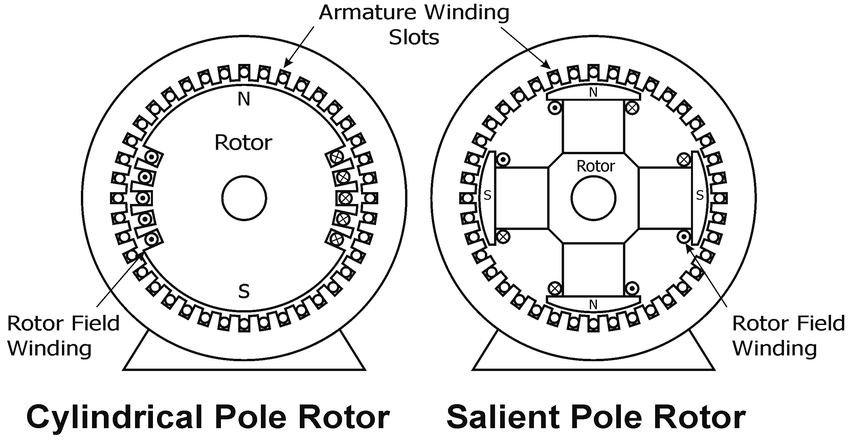
\includegraphics[width=0.5\linewidth]{imagenes/polosaliente_cilindrico.png}
    \caption{Diagrama representativo de un rotor genérico de polos no-saliente (arriba) y un rotor de polos salientes (debajo)\cite{estimation_excitation}}
    \label{fig:polos_saliente_cilindrico}
\end{figure}

\textbf{2. Migración de Propiedades Dinámicas (Análisis de Autovalores)} \mbox{}\\
Para evaluar el impacto dinámico, se analiza la migración de los polos del sistema LPV (los autovalores de la matriz $\bm{A}_o$). Se fija un punto de operación nominal de velocidad ($\omega_{m,o}$), corriente de cuadratura ($I^r_{qs,o}$) y temperatura ($T_s^\circ = T_{amb}^\circ = 25\,^\circ$C), y se realiza un barrido del parámetro $I^r_{ds,o}$ desde la zona de debilitamiento hasta la zona de reforzamiento de campo.

Sustituyendo estos valores en la matriz Jacobiana $\bm{A}_o$ analítica deducida previamente, se obtienen los autovalores para cada caso. Los resultados numéricos más relevantes se resumen en los Cuadros \ref{tab:migracion_polos} (debilitamiento) y \ref{tab:migracion_polos_reforzamiento} (reforzamiento). Cabe aclarar que este barrido paramétrico del modelo LPV se evalúa a la temperatura ambiente $T_s^\circ = 25\,^\circ$C, mientras que el modelo LTI de las secciones siguientes emplea la resistencia a la temperatura media de operación $R_{s0}=1{,}058\ \Omega$ (a $\approx 29{,}5\,^\circ$C); de allí las pequeñas diferencias en los polos rápidos entre ambos análisis.


\begin{table}[H]
\centering
\caption{Debilitamiento de campo ($I^r_{ds,o}<0$).}
\label{tab:migracion_polos}
\begin{tabular}{|c|c|c|c|c|c|}
\hline
$I^r_{ds,o}$ [A] & $\lambda_1$ & $\lambda_2$ & $\lambda_3$ & $\lambda_4$ & $\lambda_5$ \\
\hline
-1{,}2 & -1299{,}86 & -152{,}32 & $-92{,}75 - j\,79{,}89$ & $-92{,}75 + j\,79{,}89$ & -0{,}1081 \\
-1{,}0 & -1299{,}86 & -153{,}37 & $-92{,}24 - j\,94{,}65$ & $-92{,}24 + j\,94{,}65$ & -0{,}0921 \\
-0{,}8 & -1299{,}86 & -154{,}08 & $-91{,}90 - j\,107{,}54$ & $-91{,}90 + j\,107{,}54$ & -0{,}0800 \\
-0{,}6 & -1299{,}86 & -154{,}58 & $-91{,}65 - j\,119{,}20$ & $-91{,}65 + j\,119{,}20$ & -0{,}0705 \\
-0{,}4 & -1299{,}86 & -154{,}96 & $-91{,}47 - j\,129{,}98$ & $-91{,}47 + j\,129{,}98$ & -0{,}0629 \\
\hline
\end{tabular}
\end{table}

\begin{table}[H]
\centering
\caption{Reforzamiento de campo ($I^r_{ds,o}>0$).}
\label{tab:migracion_polos_reforzamiento}
\begin{tabular}{|c|c|c|c|c|c|}
\hline
$I^r_{ds,o}$ [A] & $\lambda_1$ & $\lambda_2$ & $\lambda_3$ & $\lambda_4$ & $\lambda_5$ \\
\hline
0{,}2 & -1299{,}86 & -155{,}70 & $-91{,}11 - j\,158{,}83$ & $-91{,}11 + j\,158{,}83$ & -0{,}0472 \\
0{,}4 & -1299{,}86 & -155{,}86 & $-91{,}03 - j\,167{,}63$ & $-91{,}03 + j\,167{,}63$ & -0{,}0434 \\
0{,}6 & -1299{,}86 & -156{,}00 & $-90{,}96 - j\,176{,}12$ & $-90{,}96 + j\,176{,}12$ & -0{,}0402 \\
0{,}8 & -1299{,}86 & -156{,}12 & $-90{,}90 - j\,184{,}35$ & $-90{,}90 + j\,184{,}35$ & -0{,}0375 \\
1{,}0 & -1299{,}86 & -156{,}22 & $-90{,}85 - j\,192{,}36$ & $-90{,}85 + j\,192{,}36$ & -0{,}0351 \\
\hline
\end{tabular}
\end{table}

A partir de la evaluación numérica de la matriz Jacobiana, se desprenden las siguientes conclusiones sobre la migración de propiedades:
\begin{enumerate}
    \item \textbf{Frecuencia de oscilación:} La variación de $I^r_{ds,o}$ afecta drásticamente a los términos cruzados electromecánicos en la matriz $\bm{A}_o$. Esto se traduce en una variación significativa de la parte imaginaria de los polos dominantes complejos conjugados. A medida que se pasa de debilitamiento a reforzamiento (aumenta $I^r_{ds,o}$), la frecuencia natural de oscilación del sistema aumenta.
    \item \textbf{Estabilidad global:} La parte real de los polos dominantes complejos conjugados (que dicta el amortiguamiento absoluto) se mantiene prácticamente inalterada ante los cambios de $I^r_{ds,o}$. Esto demuestra que inyectar corriente en el eje directo no compromete severamente la estabilidad a lazo abierto del sistema.
    \item \textbf{Dinámica rápida:} Los polos puramente reales asociados a la dinámica eléctrica rápida y a la dinámica térmica lenta permanecen virtualmente invariantes frente a los cambios en el punto de operación de $I^r_{ds,o}$.
\end{enumerate}

Estas tendencias se visualizan en las Fig.~\ref{fig:migracion_ids_full} y \ref{fig:migracion_ids_zoom}, que trazan el recorrido de los autovalores del modelo LPV al barrer $I^r_{ds,o}$ desde la zona de debilitamiento hasta la de reforzamiento de campo. En cada rama, el marcador relleno señala el extremo de debilitamiento ($I^r_{ds,o}$ mínimo), el marcador con borde negro el de reforzamiento ($I^r_{ds,o}$ máximo) y el rombo rojo el punto de operación con $I^r_{ds,o}=0$.

\begin{figure}[H]
    \centering
    
\includegraphics[width=\textwidth]{imagenes/migracion_ids_1.png}
    \caption{Migración de los autovalores del modelo LPV al variar $I^r_{ds,o}$ (vista completa del plano $s$). Se aprecia que los polos reales rápidos ($\lambda_1$ y el asociado a la dinámica eléctrica) permanecen prácticamente invariantes.}
    \label{fig:migracion_ids_full}
\end{figure}

\begin{figure}[H]
    \centering
    
\includegraphics[width=\textwidth]{imagenes/migracion_ids_2.png}
    \caption{Detalle de la migración de los polos dominantes en torno al origen. El par complejo conjugado aumenta su parte imaginaria (frecuencia natural de oscilación) al crecer $I^r_{ds,o}$, mientras que su parte real (amortiguamiento absoluto) se mantiene prácticamente constante.}
    \label{fig:migracion_ids_zoom}
\end{figure}
\subsection{Funciones de Transferencia del Modelo LTI Aumentado}
A partir del modelo LTI equivalente aumentado de cuarto orden, se obtienen las funciones de transferencia desde ambas entradas ---la acción de control $v_{qs}(t)$ y la perturbación mecánica externa $T_l(t)$--- hacia la salida de posición $\theta_m(t)$.

\subsubsection{Estado inicial considerado}
El modelo LTI aumentado es un modelo \textbf{incremental} alrededor de un punto de equilibrio. El estado inicial considerado es:
\begin{equation}
    \bm{x}_{aug}(0) = \begin{bmatrix} \theta_m(0) \\ \omega_m(0) \\ i_{qs}^r(0) \\ i_{ds}^r(0) \end{bmatrix} = \begin{bmatrix} 0 \\ 0 \\ 0 \\ 0 \end{bmatrix}
\end{equation}
Además, dado que el torque de carga $T_l(t)$ se trata como perturbación externa del modelo, no aparece ningún término no lineal dependiente de $\sin(\theta_m/r)$ en la matriz de estado. La resistencia del estator se considera constante ($R_s = R_{s0}$) por el desacoplamiento térmico.

\subsubsection{Obtención de las funciones de transferencia}
Las funciones de transferencia se calculan mediante la expresión general:
\begin{equation}
    G(s) = \bm{C}(s\bm{I} - \bm{A})^{-1}\bm{B}
\end{equation}

Dado que el estado $i_{ds}^r$ está completamente desacoplado (como se demostrará en la sección siguiente), es suficiente trabajar con el subsistema nominal de tercer orden. Aplicando la transformada de Laplace (con condiciones iniciales nulas) a las ecuaciones escalares del modelo nominal:
\begin{equation}
\begin{cases}
    s\,\Theta_m(s) = \Omega_m(s) \\[6pt]
    s\,\Omega_m(s) = \dfrac{1}{J_{eq}}\left[\dfrac{3 P_p \lambda'^r_m}{2} I_{qs}^r(s) - b_{eq}\,\Omega_m(s) - \dfrac{1}{r}\,T_l(s)\right] \\[6pt]
    s\,I_{qs}^r(s) = \dfrac{1}{L_q}\left[-P_p \lambda'^r_m\,\Omega_m(s) - R_{s0}\,I_{qs}^r(s) + V_{qs}(s)\right]
\end{cases}
\end{equation}

De la tercera ecuación se despeja $I_{qs}^r(s)$:
\begin{equation}\label{eq:iqs_despejada}
    I_{qs}^r(s) = \frac{V_{qs}(s) - P_p \lambda'^r_m\,\Omega_m(s)}{L_q\,s + R_{s0}}
\end{equation}

Sustituyendo \eqref{eq:iqs_despejada} en la segunda ecuación y agrupando:
\begin{equation}
    \left(J_{eq}\,s + b_{eq}\right)\Omega_m(s) = \frac{3 P_p \lambda'^r_m}{2} \cdot \frac{V_{qs}(s) - P_p \lambda'^r_m\,\Omega_m(s)}{L_q\,s + R_{s0}} - \frac{1}{r}\,T_l(s)
\end{equation}

Multiplicando ambos miembros por $(L_q\,s + R_{s0})$ y reordenando:
\begin{equation}
    \left[(J_{eq}\,s + b_{eq})(L_q\,s + R_{s0}) + \frac{3 P_p^2 {\lambda'^r_m}^2}{2}\right]\Omega_m(s) = \frac{3 P_p \lambda'^r_m}{2}\,V_{qs}(s) - \frac{L_q\,s + R_{s0}}{r}\,T_l(s)
\end{equation}

Finalmente, dado que $\Theta_m(s) = \Omega_m(s)/s$, y expandiendo el término entre corchetes se obtiene el denominador común:
\begin{equation}
    \Delta(s) = s\left[J_{eq} L_q\,s^2 + (b_{eq} L_q + J_{eq} R_{s0})\,s + b_{eq} R_{s0} + \frac{3 P_p^2 {\lambda'^r_m}^2}{2}\right]
\end{equation}

donde el factor $s$ proviene de la integración $\Theta_m = \Omega_m / s$. Dividiendo numerador y denominador por $J_{eq} L_q$ se obtienen las expresiones finales.

\vspace{0.3cm}

El polinomio característico del modelo aumentado es:
\begin{equation}
    \det(s\bm{I} - \bm{A}_{aug}) = \underbrace{\left(s + \frac{R_{s0}}{L_d}\right)}_{\text{Polo de } i_{ds}^r} \cdot \underbrace{\left[ s^3 + \left(\frac{b_{eq}}{J_{eq}} + \frac{R_{s0}}{L_q}\right)s^2 + \left(\frac{b_{eq} R_{s0}}{J_{eq} L_q} + \frac{3 P_p^2 {\lambda'^r_m}^2}{2 J_{eq} L_q}\right)s \right]}_{\Delta(s) \text{ --- Polinomio del subsistema nominal}}
\end{equation}

Sin embargo, al evaluar la resolvente $(s\bm{I}-\bm{A})^{-1}$ y proyectar sobre las columnas de entrada $\bm{B_c}$ y $\bm{B_d}$, el factor $(s + R_{s0}/L_d)$ se \textbf{cancela} en ambas funciones de transferencia. Esto se debe a que el estado $i_{ds}^r$ no es excitado por ninguna de las dos entradas ($B_c(4) = B_d(4) = 0$) y no es observado por la salida ($C(4) = 0$). Por tanto, las funciones de transferencia resultan de \textbf{orden 3}, con denominador $\Delta(s)$:

\vspace{0.3cm}
\textbf{Función de transferencia de control} ($v_{qs} \to \theta_m$):
\begin{equation} \label{eq:tf_vqs}
\boxed{
    G_1(s) = \frac{\Theta_m(s)}{V_{qs}(s)} = \frac{\dfrac{3 P_p \lambda'^r_m}{2 J_{eq} L_q}}{s^3 + \left(\dfrac{b_{eq}}{J_{eq}} + \dfrac{R_{s0}}{L_q}\right)s^2 + \left(\dfrac{b_{eq} R_{s0}}{J_{eq} L_q} + \dfrac{3 P_p^2 {\lambda'^r_m}^2}{2 J_{eq} L_q}\right)s}
}
\end{equation}

\vspace{0.3cm}
\textbf{Función de transferencia de perturbación} ($T_l \to \theta_m$):
\begin{equation} \label{eq:tf_Tl}
\boxed{
    G_2(s) = \frac{\Theta_m(s)}{T_l(s)} = \frac{-\dfrac{1}{r J_{eq}}\left(s + \dfrac{R_{s0}}{L_q}\right)}{s^3 + \left(\dfrac{b_{eq}}{J_{eq}} + \dfrac{R_{s0}}{L_q}\right)s^2 + \left(\dfrac{b_{eq} R_{s0}}{J_{eq} L_q} + \dfrac{3 P_p^2 {\lambda'^r_m}^2}{2 J_{eq} L_q}\right)s}
}
\end{equation}

Ambas funciones de transferencia comparten el mismo polinomio característico $\Delta(s)$, el cual presenta un polo en el origen ($s=0$) correspondiente a la integración cinemática inherente de velocidad a posición. Este polo no representa un modo físico de almacenamiento de energía, sino la acumulación de la coordenada de posición. Por ello, $\theta_m$ se interpreta aquí como una cuasi variable de estado conveniente para el posterior diseño del controlador de posición.

Notar que $G_2(s)$ posee un \textbf{cero} en $s = -R_{s0}/L_q$, que coincide con el polo eléctrico del eje $q$. Esto se interpreta físicamente como: ante una perturbación de torque de carga, la corriente $i_{qs}^r$ reacciona inicialmente absorbiendo parte del impacto, atenuando la transmisión del disturbio hacia la posición en frecuencias altas.

\subsubsection{Estado interno no reflejado en las funciones de transferencia}
El estado $i_{ds}^r$ (cuarto estado del modelo aumentado) \textbf{no aporta ni se ve reflejado} en ninguna de las funciones de transferencia obtenidas. Formalmente, esto se verifica analizando las propiedades estructurales del sistema:

\begin{enumerate}
    \item \textbf{No controlabilidad:} Ninguna de las entradas ($v_{qs}$, $T_l$) excita al estado $i_{ds}^r$, ya que las componentes correspondientes de las matrices de entrada son nulas: $B_c(4) = 0$ y $B_d(4) = 0$.
    \item \textbf{No observabilidad:} La salida $\theta_m$ no depende de $i_{ds}^r$, ya que $C(4) = 0$.
    \item \textbf{Desacoplamiento dinámico:} La cuarta fila de $\bm{A}$ solo contiene el término $-R_{s0}/L_d$ en la diagonal, sin acoplamientos con los demás estados. La dinámica de $i_{ds}^r$ es completamente autónoma.
\end{enumerate}

Consecuentemente, el polo $\lambda_4 = -R_{s0}/L_d$ del sistema en espacio de estados se cancela algebraicamente al convertir a función de transferencia. La dinámica de $i_{ds}^r$ es puramente una \textbf{respuesta libre}:
\begin{equation}
    i_{ds}^r(t) = i_{ds}^r(0) \, e^{-\frac{R_{s0}}{L_d} t}
\end{equation}
que solo se manifiesta si la condición inicial es no nula, decayendo exponencialmente con constante de tiempo $\tau_d = L_d / R_{s0}$. Esto confirma que el \textbf{modelo nominal de tercer orden} $\bm{x}_{LTI} = [\theta_m, \omega_m, i_{qs}^r]^T$ es suficiente para caracterizar completamente la relación entrada-salida del sistema.

\subsection{Análisis de Estabilidad a Lazo Abierto}

\subsubsection{Autovalores del modelo aumentado}
Los autovalores del sistema se obtienen a partir del polinomio característico de la matriz $\bm{A}_{aug}$ (4$\times$4). Como se demostró en la sección anterior, este se factoriza en dos términos independientes:
\begin{equation}
    \det(s\bm{I} - \bm{A}_{aug}) = \underbrace{\left(s + \frac{R_{s0}}{L_d}\right)}_{\lambda_4} \cdot \underbrace{s}_{\lambda_1} \cdot \underbrace{\left(s^2 + a_2\,s + a_1\right)}_{\lambda_{2,3}}
\end{equation}
donde los coeficientes del polinomio cuadrático son:
\begin{equation}
    a_2 = \frac{b_{eq}}{J_{eq}} + \frac{R_{s0}}{L_q}, \qquad a_1 = \frac{b_{eq} R_{s0}}{J_{eq} L_q} + \frac{3 P_p^2 {\lambda'^r_m}^2}{2 J_{eq} L_q}
\end{equation}

Evaluando numéricamente con los parámetros nominales ($m_l = 0$, $J_{l,nom} = 0{,}0833$ kg$\cdot$m$^2$):

\begin{table}[H]
\centering
\caption{Autovalores del modelo LTI aumentado a lazo abierto (parámetros nominales).}
\label{tab:autovalores_LA}
\renewcommand{\arraystretch}{1.4}
\begin{tabular}{|c|c|c|c|c|}
\hline
\textbf{Autovalor} & \textbf{Valor} & \textbf{Subsistema} & $\boldsymbol{\omega_n}$ \textbf{[rad/s]} & $\boldsymbol{\zeta}$ \\
\hline
$\lambda_1$ & $0$ & Cinemático de posición & --- & --- \\
\hline
$\lambda_{2,3}$ & $-91{,}7 \pm j\,148{,}0$ & Electromecánico & $174{,}1$ & $0{,}527$ \\
\hline
$\lambda_4$ & $-160{,}3$ & Residual $i_{ds}^r$ & --- & $\tau_d = 6{,}24$ ms \\
\hline
\end{tabular}
\end{table}

\textbf{Identificación física de cada autovalor:} \mbox{}

\begin{itemize}
    \item \textbf{$\lambda_1 = 0$ (Polo en el origen):} Corresponde a la relación cinemática $\dot{\theta}_m = \omega_m$. La posición es la integral de la velocidad y no almacena energía por sí misma, por lo que este polo se interpreta como un integrador cinemático asociado a una cuasi variable de estado. Su inclusión resulta conveniente para el diseño del controlador de posición, pero no modifica la estabilidad física del subsistema electromecánico.

    \item \textbf{$\lambda_{2,3} = -91{,}7 \pm j\,148{,}0$ (Par complejo conjugado):} Representan el \textbf{modo electromecánico acoplado} entre la corriente $i_{qs}^r$ y la velocidad $\omega_m$. La parte imaginaria indica un comportamiento oscilatorio subamortiguado ($\zeta \approx 0{,}53$), producto del intercambio de energía entre el campo magnético ($L_q$, $\lambda'^r_m$) y la inercia mecánica ($J_{eq}$). La frecuencia de oscilación amortiguada es $\omega_d = 148{,}0$ rad/s ($\approx 23{,}6$ Hz), y la envolvente decae con constante de tiempo $\tau_{em} = 1/91{,}7 \approx 10{,}9$ ms.

    \item \textbf{$\lambda_4 = -R_{s0}/L_d = -160{,}3$ rad/s (Polo real negativo):} Corresponde a la dinámica residual autónoma de $i_{ds}^r$. Como se demostró, este polo \textbf{no aparece} en las funciones de transferencia. Su constante de tiempo es $\tau_d = L_d/R_{s0} \approx 6{,}24$ ms.
\end{itemize}

\subsubsection{Ceros de las funciones de transferencia}

\begin{itemize}
    \item \textbf{$G_1(s) = \theta_m / v_{qs}$:} No posee ceros finitos. Es un sistema de \textbf{fase mínima} puro de tipo 1 con exceso polar de 3. La respuesta ante un escalón de tensión será una rampa modulada por la dinámica oscilatoria de los polos electromecánicos.

    \item \textbf{$G_2(s) = \theta_m / T_l$:} Posee un cero real negativo en:
    \begin{equation}
        z_1 = -\frac{R_{s0}}{L_q} = -182{,}4 \text{ rad/s} \qquad (\tau_z = 5{,}48 \text{ ms})
    \end{equation}
    Este cero se ubica muy cerca del polo electromecánico dominante. Físicamente, representa que el subsistema eléctrico ($L_q$, $R_{s0}$) ``absorbe'' parcialmente las perturbaciones de torque antes de que estas se transmitan completamente a la posición, actuando como un filtro natural de alta frecuencia sobre la perturbación.
\end{itemize}

\subsubsection{Estabilidad}

\textbf{Estabilidad interna del subsistema físico:} \mbox{} \\
El modelo LTI aumentado posee el par electromecánico $\lambda_{2,3}$ y el polo residual $\lambda_4$ con parte real estrictamente negativa. Por lo tanto, las variables que almacenan energía o representan dinámica física propia del accionamiento ($\omega_m$, $i_{qs}^r$ e $i_{ds}^r$) son estables y convergen a valores estacionarios finitos ante entradas acotadas.
En este sentido, el sistema físico se considera estable; el polo en el origen no se contabiliza como un modo dinámico energético.

\textbf{Rol del polo en el origen:} \mbox{} \\
El autovalor $\lambda_1=0$ proviene exclusivamente de la relación cinemática $\dot{\theta}_m=\omega_m$. No se lo interpreta como una pérdida de estabilidad del sistema físico, ya que la posición angular no almacena energía; actúa como una coordenada acumulada, o cuasi variable de estado, incorporada porque resulta necesaria para formular el problema de control de posición.

\textbf{Acotación de la coordenada de posición:} \mbox{} \\
Si se aplica una tensión o un torque perturbador constante en lazo abierto, la velocidad puede alcanzar un valor estacionario no nulo y, por integración cinemática, la posición puede crecer como rampa. Esto describe una deriva de la coordenada de posición en ausencia de realimentación, no una pérdida de estabilidad del subsistema electromecánico. El controlador PID que se diseñará más adelante se incorpora precisamente para regular esa coordenada acumulada.

\begin{figure}[H]
    \centering
    
\includegraphics[width=\textwidth]{imagenes/polos_ceros_LA.png}
    \caption{Mapa de polos (cuadrados sólidos) y ceros (círculos vacíos) a lazo abierto para ambas funciones de transferencia del modelo LTI aumentado. El polo cancelado de $i_{ds}^r$ se indica con rombo rojo.}
    \label{fig:polos_ceros_LA}
\end{figure}

\subsubsection{Migración de propiedades ante variación de \texorpdfstring{$R_s$}{Rs}}
La resistencia del estator varía con la temperatura según $R_s\big(T_s^\circ(t)\big)=R_{sREF}\big[1+\alpha_{Cu}\big(T_s^\circ(t)-T_{sREF}^\circ\big)\big]$. Para evaluar su efecto sobre la dinámica del modelo LTI, se realiza un barrido en el rango $[0{,}8\,R_{sREF},\; 1{,}2\,R_{sREF}] = [0{,}816;\ 1{,}224]\ \Omega$ (con $R_{sREF}=1{,}02\ \Omega$); la fila resaltada corresponde al valor más próximo a la resistencia de operación $R_{s0}\approx 1{,}058\ \Omega$.

\begin{table}[H]
\centering
\caption{Migración de polos y ceros ante variación de $R_s$.}
\label{tab:migracion_Rs}
\renewcommand{\arraystretch}{1.2}
\footnotesize
\begin{tabular}{|c|c|c|c|c|}
\hline
$R_s$ [$\Omega$] & Polos $\lambda_{2,3}$ & Cero $G_2$ & $\omega_n$ [rad/s] & $\zeta$ \\
\hline
0{,}816 & $-70{,}9 \pm j\,158{,}9$ & $-140{,}69$ & $174{,}0$ & $0{,}407$ \\
0{,}850 & $-73{,}8 \pm j\,157{,}6$ & $-146{,}55$ & $174{,}0$ & $0{,}424$ \\
0{,}884 & $-76{,}8 \pm j\,156{,}2$ & $-152{,}41$ & $174{,}0$ & $0{,}441$ \\
0{,}918 & $-79{,}7 \pm j\,154{,}7$ & $-158{,}28$ & $174{,}0$ & $0{,}458$ \\
0{,}952 & $-82{,}6 \pm j\,153{,}2$ & $-164{,}14$ & $174{,}1$ & $0{,}475$ \\
0{,}986 & $-85{,}6 \pm j\,151{,}6$ & $-170{,}00$ & $174{,}1$ & $0{,}491$ \\
1{,}020 & $-88{,}5 \pm j\,149{,}9$ & $-175{,}86$ & $174{,}1$ & $0{,}508$ \\
\textbf{1{,}054} & $\mathbf{-91{,}4 \pm j\,148{,}2}$ & $\mathbf{-181{,}72}$ & $\mathbf{174{,}1}$ & $\mathbf{0{,}525}$ \\
1{,}088 & $-94{,}3 \pm j\,146{,}4$ & $-187{,}59$ & $174{,}1$ & $0{,}542$ \\
1{,}122 & $-97{,}3 \pm j\,144{,}5$ & $-193{,}45$ & $174{,}2$ & $0{,}559$ \\
1{,}156 & $-100{,}2 \pm j\,142{,}5$ & $-199{,}31$ & $174{,}2$ & $0{,}575$ \\
1{,}190 & $-103{,}1 \pm j\,140{,}4$ & $-205{,}17$ & $174{,}2$ & $0{,}592$ \\
1{,}224 & $-106{,}1 \pm j\,138{,}2$ & $-211{,}03$ & $174{,}2$ & $0{,}609$ \\
\hline
\end{tabular}
\end{table}

Del análisis se concluye:
\begin{itemize}
    \item La \textbf{frecuencia natural} $\omega_n$ permanece prácticamente constante ($\approx 174$ rad/s), ya que depende principalmente del acoplamiento electromecánico $P_p\lambda'^r_m$ y la inercia $J_{eq}$, no de $R_s$.
    \item El \textbf{amortiguamiento} $\zeta$ aumenta con $R_s$ (de $0{,}41$ a $0{,}61$), lo que se explica porque una mayor resistencia disipa más rápidamente la energía almacenada en el campo magnético.
    \item El \textbf{cero} de $G_2(s)$ migra proporcionalmente a $R_s$ ($z = -R_s/L_q$), desplazándose hacia la izquierda con el aumento de temperatura.
\end{itemize}

\begin{figure}[H]
    \centering
    
\includegraphics[width=\textwidth]{imagenes/migracion_Rs.png}
    \caption{Migración de polos y ceros en el plano $s$ (izquierda) y variación de $\omega_n$ y $\zeta$ (derecha) ante cambios en $R_s$.}
    \label{fig:migracion_Rs}
\end{figure}

\subsubsection{Migración de propiedades ante variación de carga ($m_l$)}
La masa de carga útil $m_l \in [0,\; 1{,}5]$ kg modifica la inercia equivalente $J_{eq} = J_m + J_l/r^2$ y el coeficiente gravitacional $k_l$. Al aumentar $m_l$, la inercia crece y el acoplamiento electromecánico se ``diluye'', modificando los autovalores.

\begin{table}[H]
\centering
\caption{Migración de polos ante variación de masa de carga $m_l$.}
\label{tab:migracion_ml}
\renewcommand{\arraystretch}{1.2}
\footnotesize
\begin{tabular}{|c|c|c|c|c|}
\hline
$m_l$ [kg] & $J_{eq}$ [kg$\cdot$m$^2$] & Polos $\lambda_{2,3}$ & $\omega_n$ [rad/s] & $\zeta$ \\
\hline
\textbf{0{,}00} & $\mathbf{1{,}98 \times 10^{-5}}$ & $\mathbf{-91{,}7 \pm j\,148{,}0}$ & $\mathbf{174{,}1}$ & $\mathbf{0{,}527}$ \\
0{,}20 & $2{,}33 \times 10^{-5}$ & $-91{,}7 \pm j\,131{,}9$ & $160{,}6$ & $0{,}571$ \\
0{,}40 & $2{,}67 \times 10^{-5}$ & $-91{,}6 \pm j\,118{,}5$ & $149{,}8$ & $0{,}611$ \\
0{,}60 & $3{,}02 \times 10^{-5}$ & $-91{,}6 \pm j\,107{,}1$ & $140{,}9$ & $0{,}650$ \\
0{,}80 & $3{,}37 \times 10^{-5}$ & $-91{,}5 \pm j\,97{,}2$ & $133{,}5$ & $0{,}686$ \\
1{,}00 & $3{,}71 \times 10^{-5}$ & $-91{,}5 \pm j\,88{,}2$ & $127{,}1$ & $0{,}720$ \\
1{,}20 & $4{,}06 \times 10^{-5}$ & $-91{,}5 \pm j\,80{,}0$ & $121{,}5$ & $0{,}753$ \\
1{,}50 & $4{,}58 \times 10^{-5}$ & $-91{,}4 \pm j\,68{,}8$ & $114{,}4$ & $0{,}799$ \\
\hline
\end{tabular}
\end{table}

\begin{figure}[H]
    \centering
    
\includegraphics[width=\textwidth]{imagenes/migracion_ml.png}
    \caption{Migración de polos ante variación de masa de carga $m_l$ (izquierda) y variación de $\omega_n$ y $\zeta$ (derecha).}
    \label{fig:migracion_ml}
\end{figure}

Del análisis se observa que al aumentar $m_l$:
\begin{itemize}
    \item La \textbf{frecuencia natural} $\omega_n$ disminuye, ya que la mayor inercia reduce la relación torque/inercia del sistema.
    \item El \textbf{amortiguamiento} $\zeta$ aumenta, porque la fricción equivalente $b_{eq}$ se mantiene mientras la frecuencia natural baja, incrementando la relación $\zeta = a_2/(2\omega_n)$.
    \item El polo en el origen y el cero de $G_2$ permanecen invariantes frente a $m_l$.
\end{itemize}

Estas variaciones justifican la necesidad de un controlador robusto capaz de mantener el desempeño dentro de todo el rango de incertidumbre de carga.

\subsubsection{Diagramas de Bode a lazo abierto}
La Fig.~\ref{fig:bode_LA} presenta la respuesta en frecuencia de ambas funciones de transferencia. La FT de control $G_1(s)$ exhibe la pendiente de $-20$~dB/dec a bajas frecuencias característica del integrador cinemático (sistema de tipo 1), un pico resonante en torno a la frecuencia natural del par electromecánico ($\omega_n\approx174$~rad/s, $\zeta=0{,}527$) y una atenuación asintótica de $-60$~dB/dec por encima de dicha frecuencia (exceso polar de 3, con fase que va de $-90^\circ$ a $-270^\circ$). La FT de perturbación $G_2(s)$ comparte los mismos polos, pero su cero en $-R_{s0}/L_q\approx-182$~rad/s aplana la respuesta a altas frecuencias, evidenciando la atenuación natural que el subsistema eléctrico ejerce sobre el torque de carga.

\begin{figure}[H]
    \centering
    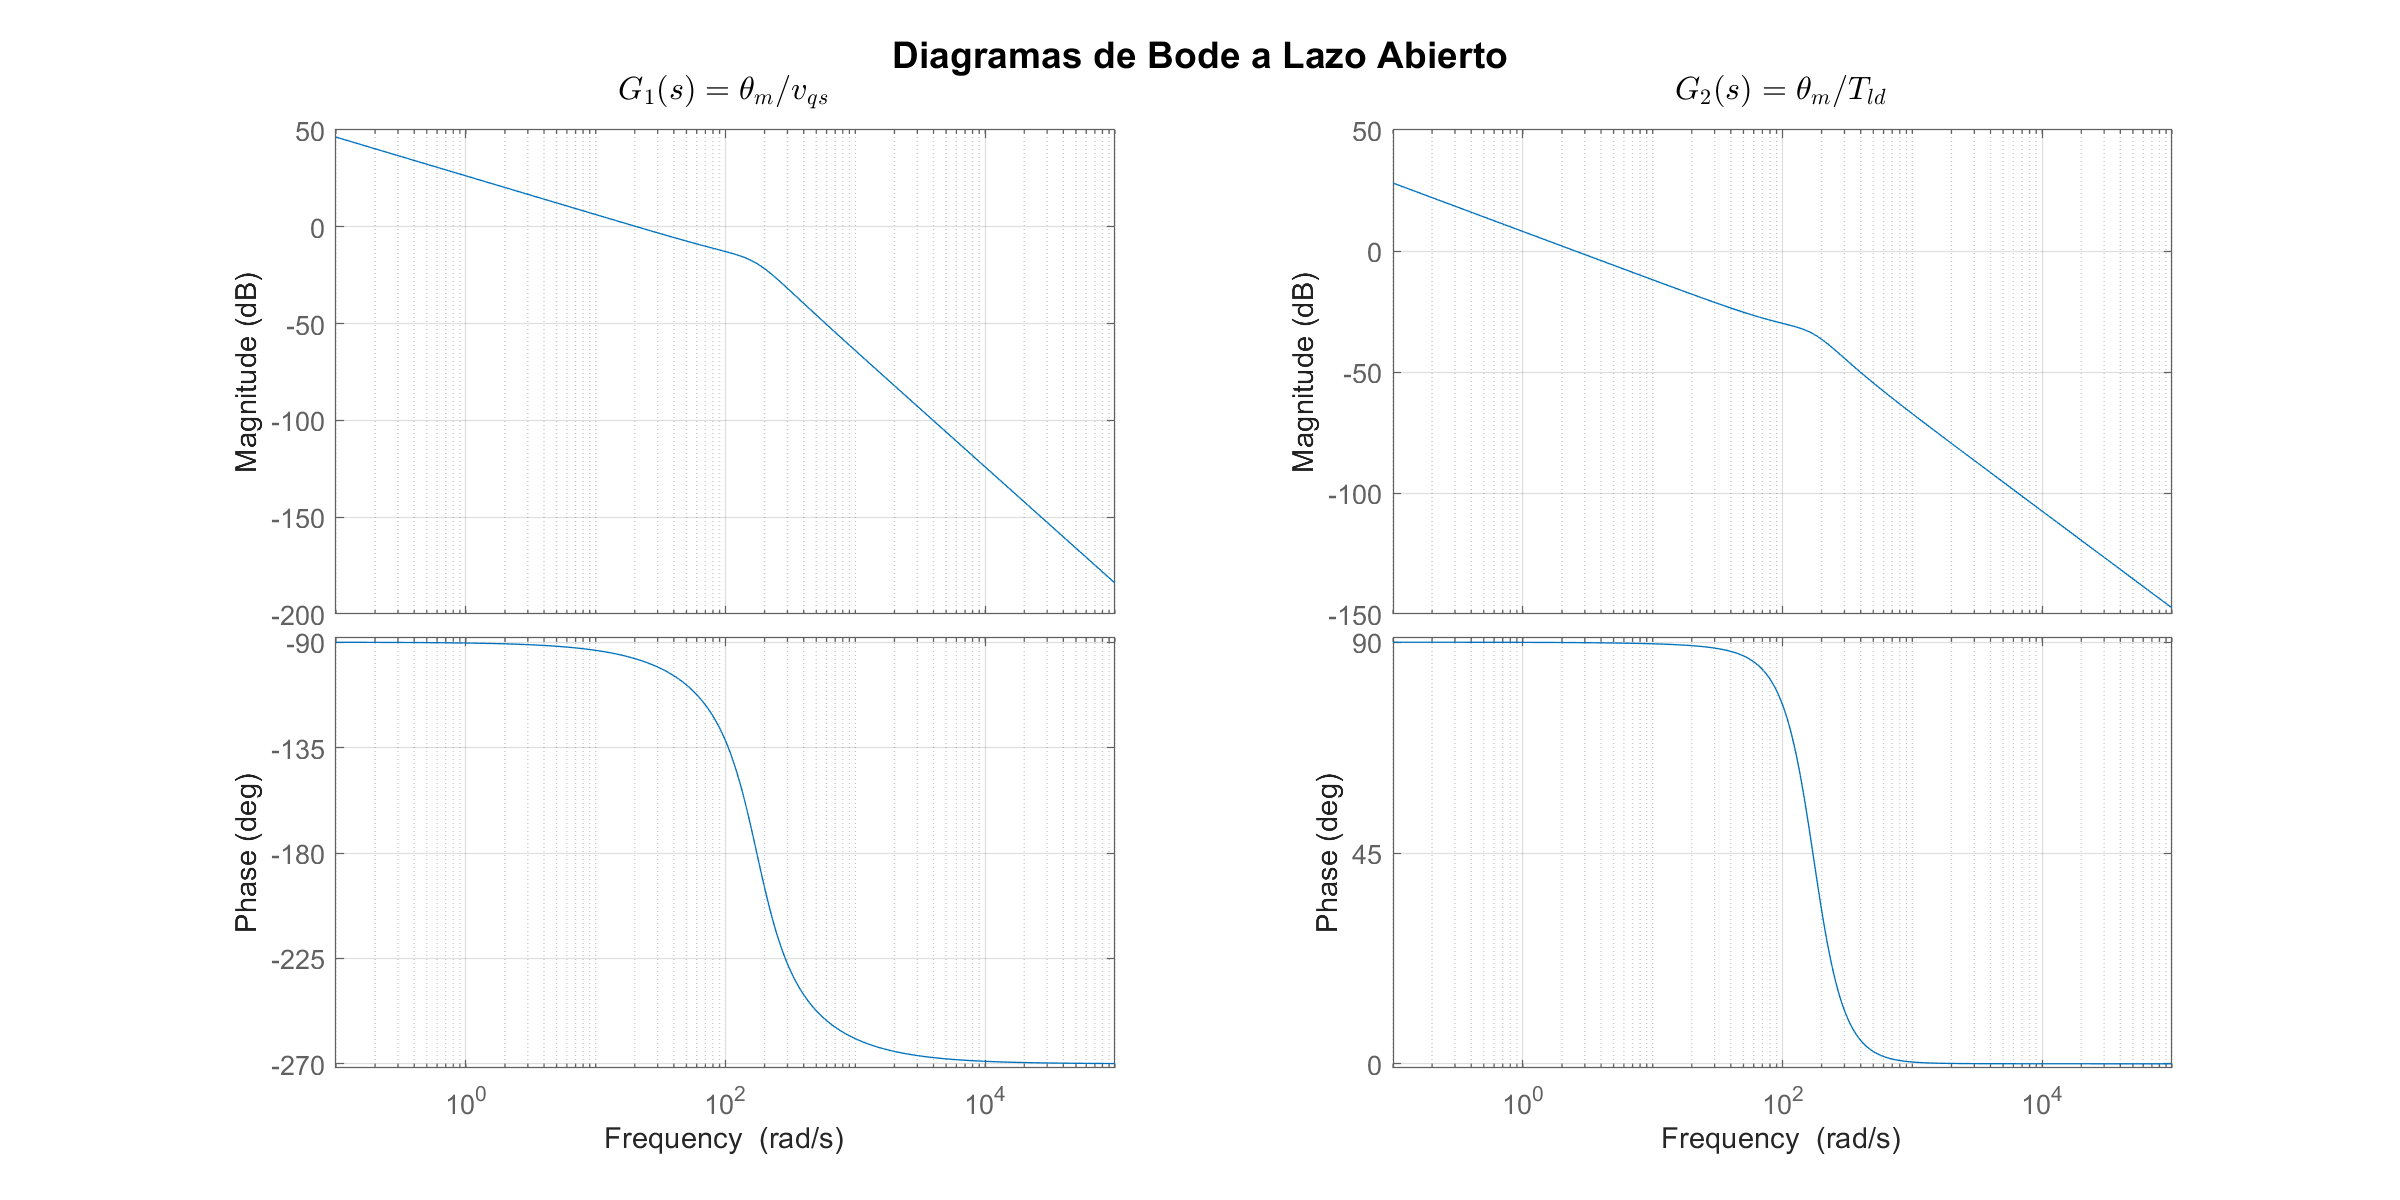
\includegraphics[width=\textwidth]{imagenes/bode_LA.png}
    \caption{Diagramas de Bode de las funciones de transferencia $G_1(s)$ y $G_2(s)$ a lazo abierto.}
    \label{fig:bode_LA}
\end{figure}

\subsection{Análisis de Observabilidad}
Se analiza si es posible reconstruir el vector de estado completo del modelo LTI aumentado a partir de la medición de una única salida escalar.

\subsubsection{Observabilidad desde \texorpdfstring{$\theta_m(t)$}{theta_m(t)} (sensor de posición)}
La matriz de observabilidad para el sistema $(\bm{A}_{aug}, \bm{C})$ con $\bm{C} = \begin{bmatrix} 1 & 0 & 0 & 0 \end{bmatrix}$ se construye como:
\begin{equation}
    \mathcal{O} = \begin{bmatrix} \bm{C} \\ \bm{C}\bm{A} \\ \bm{C}\bm{A}^2 \\ \bm{C}\bm{A}^3 \end{bmatrix}
\end{equation}

Evaluando fila por fila a partir de la estructura de $\bm{A}_{aug}$:
\begin{itemize}
    \item $\bm{C} = \begin{bmatrix} 1 & 0 & 0 & 0 \end{bmatrix}$ --- se observa $\theta_m$ directamente.
    \item $\bm{C}\bm{A} = \begin{bmatrix} 0 & 1 & 0 & 0 \end{bmatrix}$ --- se observa $\omega_m$ (derivada de $\theta_m$).
    \item $\bm{C}\bm{A}^2 = \begin{bmatrix} 0 & -\frac{b_{eq}}{J_{eq}} & \frac{3P_p\lambda'^r_m}{2J_{eq}} & 0 \end{bmatrix}$ --- combinación de $\omega_m$ e $i_{qs}^r$.
    \item $\bm{C}\bm{A}^3$: combinación que involucra $\omega_m$ e $i_{qs}^r$, pero \textbf{nunca} $i_{ds}^r$.
\end{itemize}

La cuarta columna de $\mathcal{O}$ es idénticamente nula, ya que $i_{ds}^r$ no acopla con ningún estado observable. Por lo tanto:
\begin{equation}
    \text{rango}(\mathcal{O}) = 3 < 4 = n
\end{equation}

\textbf{Conclusión:} El sistema \textbf{no es completamente observable} desde $\theta_m(t)$. El estado no observable es $i_{ds}^r$. Los tres estados restantes ($\theta_m$, $\omega_m$, $i_{qs}^r$) sí son observables, lo que permite diseñar un observador reducido para estimar $\omega_m$ e $i_{qs}^r$ a partir de la medición de posición.

Esto es consistente con el análisis de las funciones de transferencia: dado que $i_{ds}^r$ no se manifiesta en la salida $\theta_m$, es imposible reconstruirlo a partir de dicha medición.

\subsubsection{Observabilidad desde \texorpdfstring{$\omega_m(t)$}{omega_m(t)} (tacogenerador)}
Si en lugar de medir la posición se mide la velocidad angular, la matriz de salida es $\bm{C}_\omega = \begin{bmatrix} 0 & 1 & 0 & 0 \end{bmatrix}$. Evaluando:
\begin{itemize}
    \item $\bm{C}_\omega = \begin{bmatrix} 0 & 1 & 0 & 0 \end{bmatrix}$ --- se observa $\omega_m$.
    \item $\bm{C}_\omega\bm{A} = \begin{bmatrix} 0 & -\frac{b_{eq}}{J_{eq}} & \frac{3P_p\lambda'^r_m}{2J_{eq}} & 0 \end{bmatrix}$ --- combinación de $\omega_m$ e $i_{qs}^r$.
    \item $\bm{C}_\omega\bm{A}^2$: combinación de $\omega_m$ e $i_{qs}^r$.
    \item $\bm{C}_\omega\bm{A}^3$: combinación de $\omega_m$ e $i_{qs}^r$.
\end{itemize}

Nuevamente, la cuarta columna es nula ($i_{ds}^r$ sigue sin ser observable), pero además la primera columna también es nula: la posición $\theta_m$ nunca aparece en las potencias de $\bm{C}_\omega\bm{A}^k$ porque $\theta_m$ solo se acopla unidireccionalmente como integrador de $\omega_m$.

\begin{equation}
    \text{rango}(\mathcal{O}_\omega) = 2 < 4 = n
\end{equation}

\textbf{Conclusión:} Midiendo $\omega_m$ se pierden \textbf{dos} estados: $\theta_m$ e $i_{ds}^r$. La posición no es observable desde la velocidad porque la integración ``borra'' la condición inicial ---es decir, infinitas trayectorias de posición producen la misma velocidad. Por tanto, medir $\theta_m$ con un \textit{encoder} es estrictamente más informativo que medir $\omega_m$ con un tacogenerador para este sistema. Cabe recordar que, según la guía~\cite{guia_trabajo}, el sensor de posición es un encoder incremental con \textit{homing} y decodificación idealizados: la variable medida $\theta_m(t)$ es la posición angular absoluta ``rectificada'' (al girar más de una revolución), con ajuste $\theta_m \equiv 0$ (\textit{Home}) para $\theta_l \equiv 0$.

\subsection{Análisis de Controlabilidad}
Se analiza si es posible llevar el vector de estado completo a cualquier valor deseado mediante la entrada de control $v_{qs}(t)$, sin considerar la perturbación $T_l(t)$.

\subsubsection{Controlabilidad desde \texorpdfstring{$v_{qs}(t)$}{v_qs(t)}}
La matriz de controlabilidad para el sistema $(\bm{A}_{aug}, \bm{B}_c)$ con $\bm{B}_c = \begin{bmatrix} 0 & 0 & 1/L_q & 0 \end{bmatrix}^T$ es:
\begin{equation}
    \mathcal{C} = \begin{bmatrix} \bm{B}_c & \bm{A}\bm{B}_c & \bm{A}^2\bm{B}_c & \bm{A}^3\bm{B}_c \end{bmatrix}
\end{equation}

Evaluando columna por columna:
\begin{itemize}
    \item $\bm{B}_c = \begin{bmatrix} 0 \\ 0 \\ 1/L_q \\ 0 \end{bmatrix}$ --- la entrada actúa directamente sobre $i_{qs}^r$.
    \item $\bm{A}\bm{B}_c = \begin{bmatrix} 0 \\ \frac{3P_p\lambda'^r_m}{2J_{eq}L_q} \\ -\frac{R_{s0}}{L_q^2} \\ 0 \end{bmatrix}$ --- la acción se propaga a $\omega_m$ a través del torque.
    \item $\bm{A}^2\bm{B}_c$: la acción alcanza $\theta_m$ (vía la cadena $i_{qs}^r \to \omega_m \to \theta_m$).
    \item $\bm{A}^3\bm{B}_c$: combinación de los tres estados del subsistema nominal.
\end{itemize}

La cuarta fila de todas las columnas de $\mathcal{C}$ es idénticamente nula, ya que la entrada $v_{qs}$ nunca llega al estado $i_{ds}^r$ ($B_c(4) = 0$) y ningún otro estado acopla hacia $i_{ds}^r$ (la fila 4 de $\bm{A}$ es diagonal). Por lo tanto:
\begin{equation}
    \text{rango}(\mathcal{C}) = 3 < 4 = n
\end{equation}

\textbf{Conclusión:} El sistema \textbf{no es completamente controlable} desde $v_{qs}(t)$. El estado no controlable es $i_{ds}^r$.

\subsubsection{Incorporación de una entrada adicional}
El estado $i_{ds}^r$ podría controlarse si se agrega una segunda entrada manipulable: la tensión del eje directo $v_{ds}^r(t)$. En el modelo aumentado, esto equivale a extender la matriz de entrada:
\begin{equation}
    \bm{B}_{ext} = \begin{bmatrix} \bm{B}_c & \bm{B}_{ds} \end{bmatrix} =
    \begin{bmatrix}
    0 & 0 \\ 0 & 0 \\ 1/L_q & 0 \\ 0 & 1/L_d
    \end{bmatrix}
\end{equation}

Con esta extensión, la matriz de controlabilidad alcanza rango 4 y el sistema pasa a ser completamente controlable. Sin embargo, en la práctica esta entrada $v_{ds}^r$ ya está siendo utilizada por la \textbf{ley de control mínima} \eqref{eq:vds_minima} para forzar $i_{ds}^r \to 0$. Es decir, la propia estrategia de control vectorial ya ``controla'' $i_{ds}^r$ llevándola exponencialmente a cero; simplemente no lo hace a través de la estructura de realimentación de estado convencional, sino mediante la inyección de una tensión de desacoplamiento.

\subsubsection{Resumen de propiedades estructurales}

\begin{table}[H]
\centering
\caption{Resumen de controlabilidad y observabilidad del modelo LTI aumentado.}
\label{tab:ctrl_obs}
\renewcommand{\arraystretch}{1.3}
\begin{tabular}{|l|c|c|c|c|}
\hline
\textbf{Estado} & \textbf{Controlable} ($v_{qs}$) & \textbf{Observable} ($\theta_m$) & \textbf{Observable} ($\omega_m$) & \textbf{En las funciones de transferencia} \\
\hline
$\theta_m$   & Sí & Sí (directo) & No & Sí \\
$\omega_m$   & Sí & Sí           & Sí (directo) & Sí \\
$i_{qs}^r$     & Sí (directo) & Sí      & Sí & Sí \\
$i_{ds}^r$   & No & No            & No & No \\
\hline
\end{tabular}
\end{table}

El estado $i_{ds}^r$ es simultáneamente no controlable y no observable, confirmando su naturaleza de \textbf{modo oculto} del sistema. Este resultado es coherente con la cancelación polo-cero identificada en las funciones de transferencia y con el desacoplamiento estructural de la cuarta fila y columna de la matriz $\bm{A}_{aug}$.

%%%SECCION 516
\subsection{Simulación Dinámica: Modelo NL vs LTI Aumentado}
\label{sec:sim_dinamica}

Se realiza una simulación en el dominio del tiempo comparando la respuesta del \textbf{modelo no lineal completo} (6 estados, con leyes de control NL de desacoplamiento mínima y complementaria) contra el \textbf{modelo LTI aumentado} (4 estados), implementados en MATLAB/Simulink. La simulación se ejecuta para tres condiciones iniciales: $i_{ds}^r(0) \in \{0,\; +0{,}5,\; -0{,}5\}$ A, manteniendo el resto del estado inicial en cero y $T_{amb}^\circ = 25\,^\circ$C.

\subsubsection{Señales de excitación}

La consigna define una secuencia temporal de 10 eventos (escalones) que producen transitorios sucesivos. La combinación de ambas señales permite explorar los cuatro cuadrantes de operación.

\textbf{Pulso de tensión en eje $q$:}
\begin{equation}
v_{qs}^{r*}(t) = \begin{cases}
0 \text{ V} & t < 0{,}1 \text{ s} \\
+19{,}596 \text{ V} & 0{,}1 \leq t < 0{,}7 \text{ s} \\
0 \text{ V} & 0{,}7 \leq t < 1{,}1 \text{ s} \\
-19{,}596 \text{ V} & 1{,}1 \leq t < 1{,}7 \text{ s} \\
0 \text{ V} & t \geq 1{,}7 \text{ s}
\end{cases}
\end{equation}

\textbf{Doble pulso de torque de carga:}
\begin{equation}
T_{ld}(t) = \begin{cases}
0 & t < 0{,}3 \text{ s} \\
+6{,}28 \text{ N.m} & 0{,}3 \leq t < 0{,}5 \text{ s} \\
-6{,}28 \text{ N.m} & 0{,}5 \leq t < 0{,}9 \text{ s} \\
0 & 0{,}9 \leq t < 1{,}3 \text{ s} \\
+6{,}28 \text{ N.m} & 1{,}3 \leq t < 1{,}5 \text{ s} \\
-6{,}28 \text{ N.m} & 1{,}5 \leq t < 1{,}9 \text{ s} \\
0 & t \geq 1{,}9 \text{ s}
\end{cases}
\end{equation}

\begin{figure}[H]
    \centering
    
\includegraphics[width=\textwidth]{imagenes/sim_senales_entrada.png}
    \caption{Señales de excitación: consigna de tensión $v_{qs}^{r*}(t)$ y torque de carga $T_{ld}(t)$.}
    \label{fig:sim_entradas}
\end{figure}

De la secuencia se identifican 10 transitorios consecutivos, separados por los instantes de conmutación $t_{step\,1} = 0{,}1$~s, $t_{step\,2} = 0{,}3$~s, $t_{step\,3} = 0{,}5$~s, $t_{step\,4} = 0{,}7$~s, $t_{step\,5} = 0{,}9$~s, $t_{step\,6} = 1{,}1$~s, $t_{step\,7} = 1{,}3$~s, $t_{step\,8} = 1{,}5$~s, $t_{step\,9} = 1{,}7$~s, $t_{step\,10} = 1{,}9$~s. La primera mitad (Trans.~1--5) corresponde al pulso positivo de $v_{qs}^{r*}$ y la segunda mitad (Trans.~6--10) a su simétrico negativo.

\subsubsection{Modelo en Simulink}

Se construyó un modelo en Simulink con dos subsistemas en paralelo: el modelo NL completo y el modelo LTI aumentado. Ambos reciben las mismas señales de excitación.

\begin{figure}[H]
    \centering
    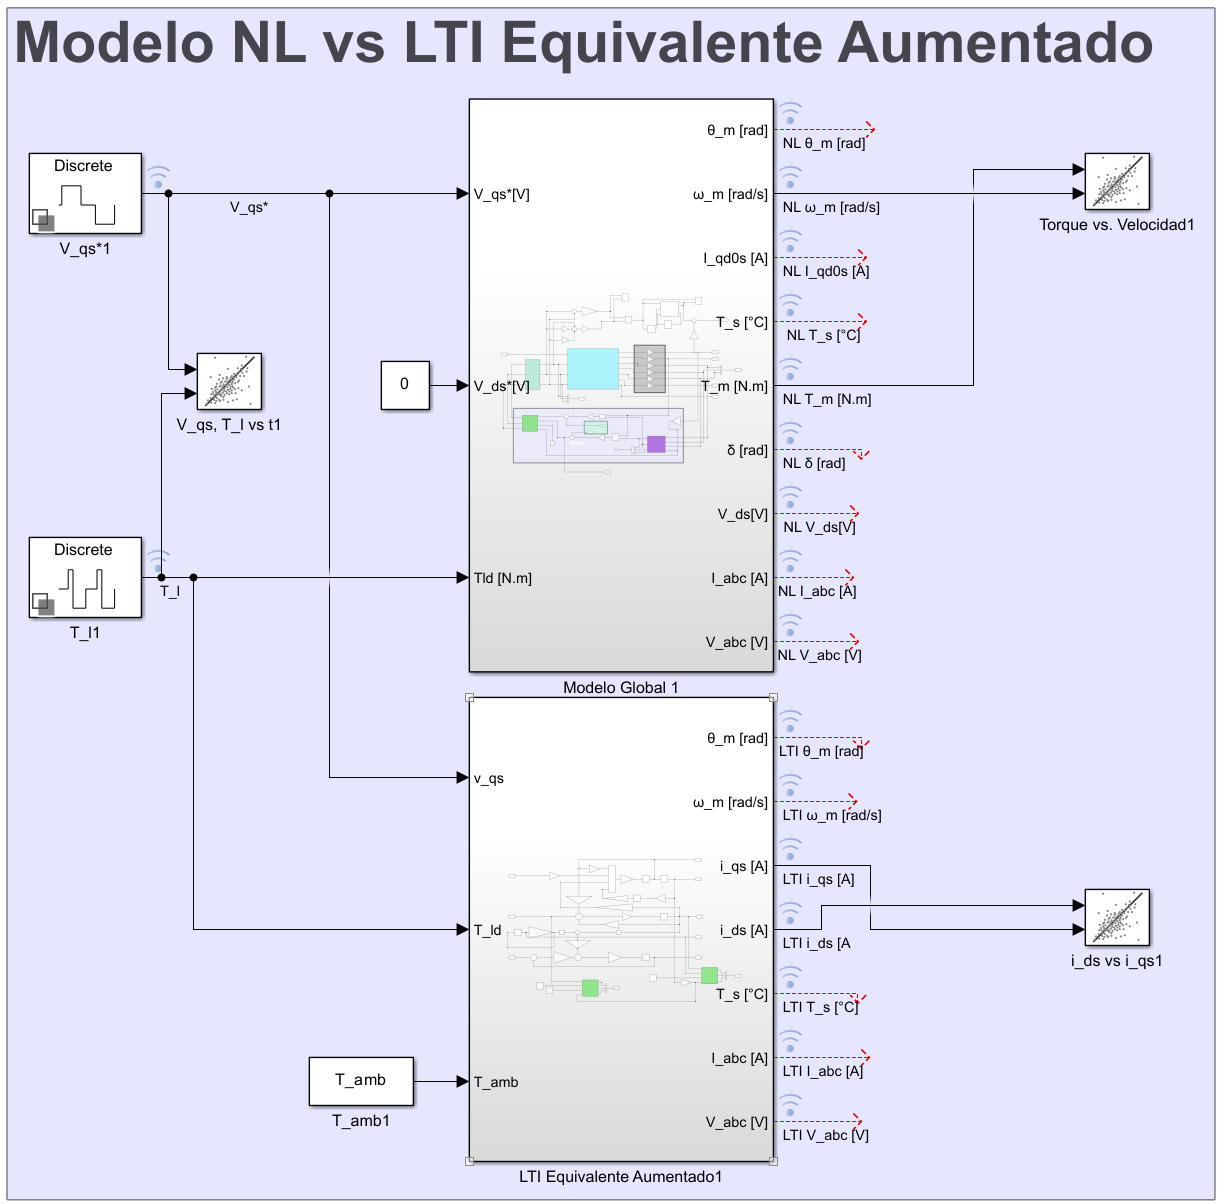
\includegraphics[width=0.5\textwidth]{imagenes/sim_diagrama_bloques.png}
    \caption{Diagrama de bloques en Simulink: modelo NL desacoplado y LTI aumentado en paralelo frente a la misma consigna $v_{qs}^{r*}$ y al mismo torque de perturbación.}
    \label{fig:simulink_diagrama}
\end{figure}

\subsubsection{Respuesta del estado interno (Sub-ítem a)}
\label{sec:sim_item_a}

Se presentan los resultados de la simulación para el caso nominal $i_{ds}^r(0) = 0$~A, comparando las salidas del modelo NL (6 estados) y del modelo LTI aumentado (4 estados) ante las mismas señales de excitación. Los efectos de $i_{ds}^r(0) \neq 0$ se analizan por separado en el Sub-ítem~c. En las siguientes simulaciones se consideró $T_{amb}^\circ=25\,^\circ$C y, en el modelo LTI aumentado, se utilizó $R_s = R_{s0} = 1{,}058\ \Omega$ constante, evaluada a la temperatura media de operación del estator ($\approx 29{,}5\,^\circ$C) y no al valor de referencia $R_{sREF}=1{,}02\ \Omega$ a $20\,^\circ$C, consistente con el desacoplamiento térmico del modelo lineal equivalente.

\textbf{Posición angular $\theta_m(t)$}

La posición angular crece como rampa durante los pulsos de tensión, consecuencia directa del integrador puro ($\dot{\theta}_m = \omega_m$). Alcanza un máximo de $\approx 242$~rad en $t \approx 0{,}7$~s, que se mantiene hasta $t \approx 1{,}1$~s (durante $v_{qs}^{r*} = 0$) y retorna hacia cero durante el pulso negativo de $v_{qs}^{r*}$. La Fig.~\ref{fig:sim_theta_m} compara ambos modelos junto con las señales de excitación, y la Fig.~\ref{fig:sim_theta_m_error} cuantifica el error de seguimiento.

\begin{figure}[H]
    \centering
    
\includegraphics[width=\textwidth]{imagenes/sim_theta_m.png}
    \caption{Posición angular $\theta_m(t)$: comparación NL (azul) vs LTI aumentado (rojo). Panel inferior: señales de excitación (torque de carga $T_l$ y consigna $v_{qs}^{r*}$).}
    \label{fig:sim_theta_m}
\end{figure}

\begin{figure}[H]
    \centering
    
\includegraphics[width=\textwidth]{imagenes/sim_theta_m_error.png}
    \caption{Error de seguimiento en $\theta_m(t)$: diferencia $\theta_m^{\mathrm{NL}}(t)-\theta_m^{\mathrm{LTI}}(t)$, acotada por debajo de $0{,}1$~rad ($<0{,}05\%$ de la excursión de $242$~rad).}
    \label{fig:sim_theta_m_error}
\end{figure}

El error de seguimiento se mantiene acotado por debajo de $0{,}1$~rad durante todo el ensayo. A diferencia de las demás variables, este error no se anula en régimen permanente sino que exhibe una deriva lenta y acumulativa: dado que $\theta_m$ es la integral de $\omega_m$, el integrador acumula las pequeñas discrepancias instantáneas de velocidad entre ambos modelos, dando lugar a un offset residual de $\approx 0{,}085$~rad al finalizar el ensayo. Este comportamiento es inherente a la presencia del integrador puro en la planta y no constituye un error de modelado.

\textbf{Velocidad angular $\omega_m(t)$.}

La velocidad está gobernada por el \textbf{modo electromecánico subamortiguado} del sistema (par de polos complejos $\lambda_{2,3} = -91{,}7 \pm j148$, $\zeta = 0{,}527$, $\omega_n = 174$~rad/s, hallado en el análisis de estabilidad a lazo abierto). Ante el escalón de $v_{qs}^{r*}$, $\omega_m$ acelera hasta su \textbf{velocidad de vacío} ($\approx +405$~rad/s para $+19{,}6$~V, valor en que la fuerza contraelectromotriz $\lambda'^r_m P_p \omega_m$ equilibra la tensión aplicada), inferior al límite nominal del motor $\omega_{m,nom}=691{,}15$~rad/s, \textbf{con un sobrepico de $\approx 14\%$} propio del amortiguamiento $\zeta = 0{,}527$ y un tiempo de establecimiento ($\pm 1\%$) de $\approx 50$~ms. No domina la constante mecánica $\tau_m = J_{eq}/b_{eq} \approx 0{,}90$~s: la realimentación electromagnética (fuerza contraelectromotriz más torque) fusiona los modos eléctrico y mecánico en una resonancia rápida ($\tau \approx 11$~ms). Durante el pulso negativo ($1{,}1$--$1{,}7$~s) la respuesta es simétrica ($\approx -405$~rad/s). La concordancia NL--LTI es excelente: el error (Fig.~\ref{fig:sim_omega_m_error}) es prácticamente nulo en régimen permanente ($<0{,}5$~rad/s) y solo presenta picos $\leq 3$~rad/s en las conmutaciones, que se extinguen en milisegundos.

\begin{figure}[H]
    \centering
    
\includegraphics[width=\textwidth]{imagenes/sim_omega_m.png}
    \caption{Velocidad angular $\omega_m(t)$: comparación NL (azul) vs LTI aumentado (rojo). Panel inferior: señales de excitación ($T_l$ y $v_{qs}^{r*}$).}
    \label{fig:sim_omega_m}
\end{figure}

\begin{figure}[H]
    \centering
    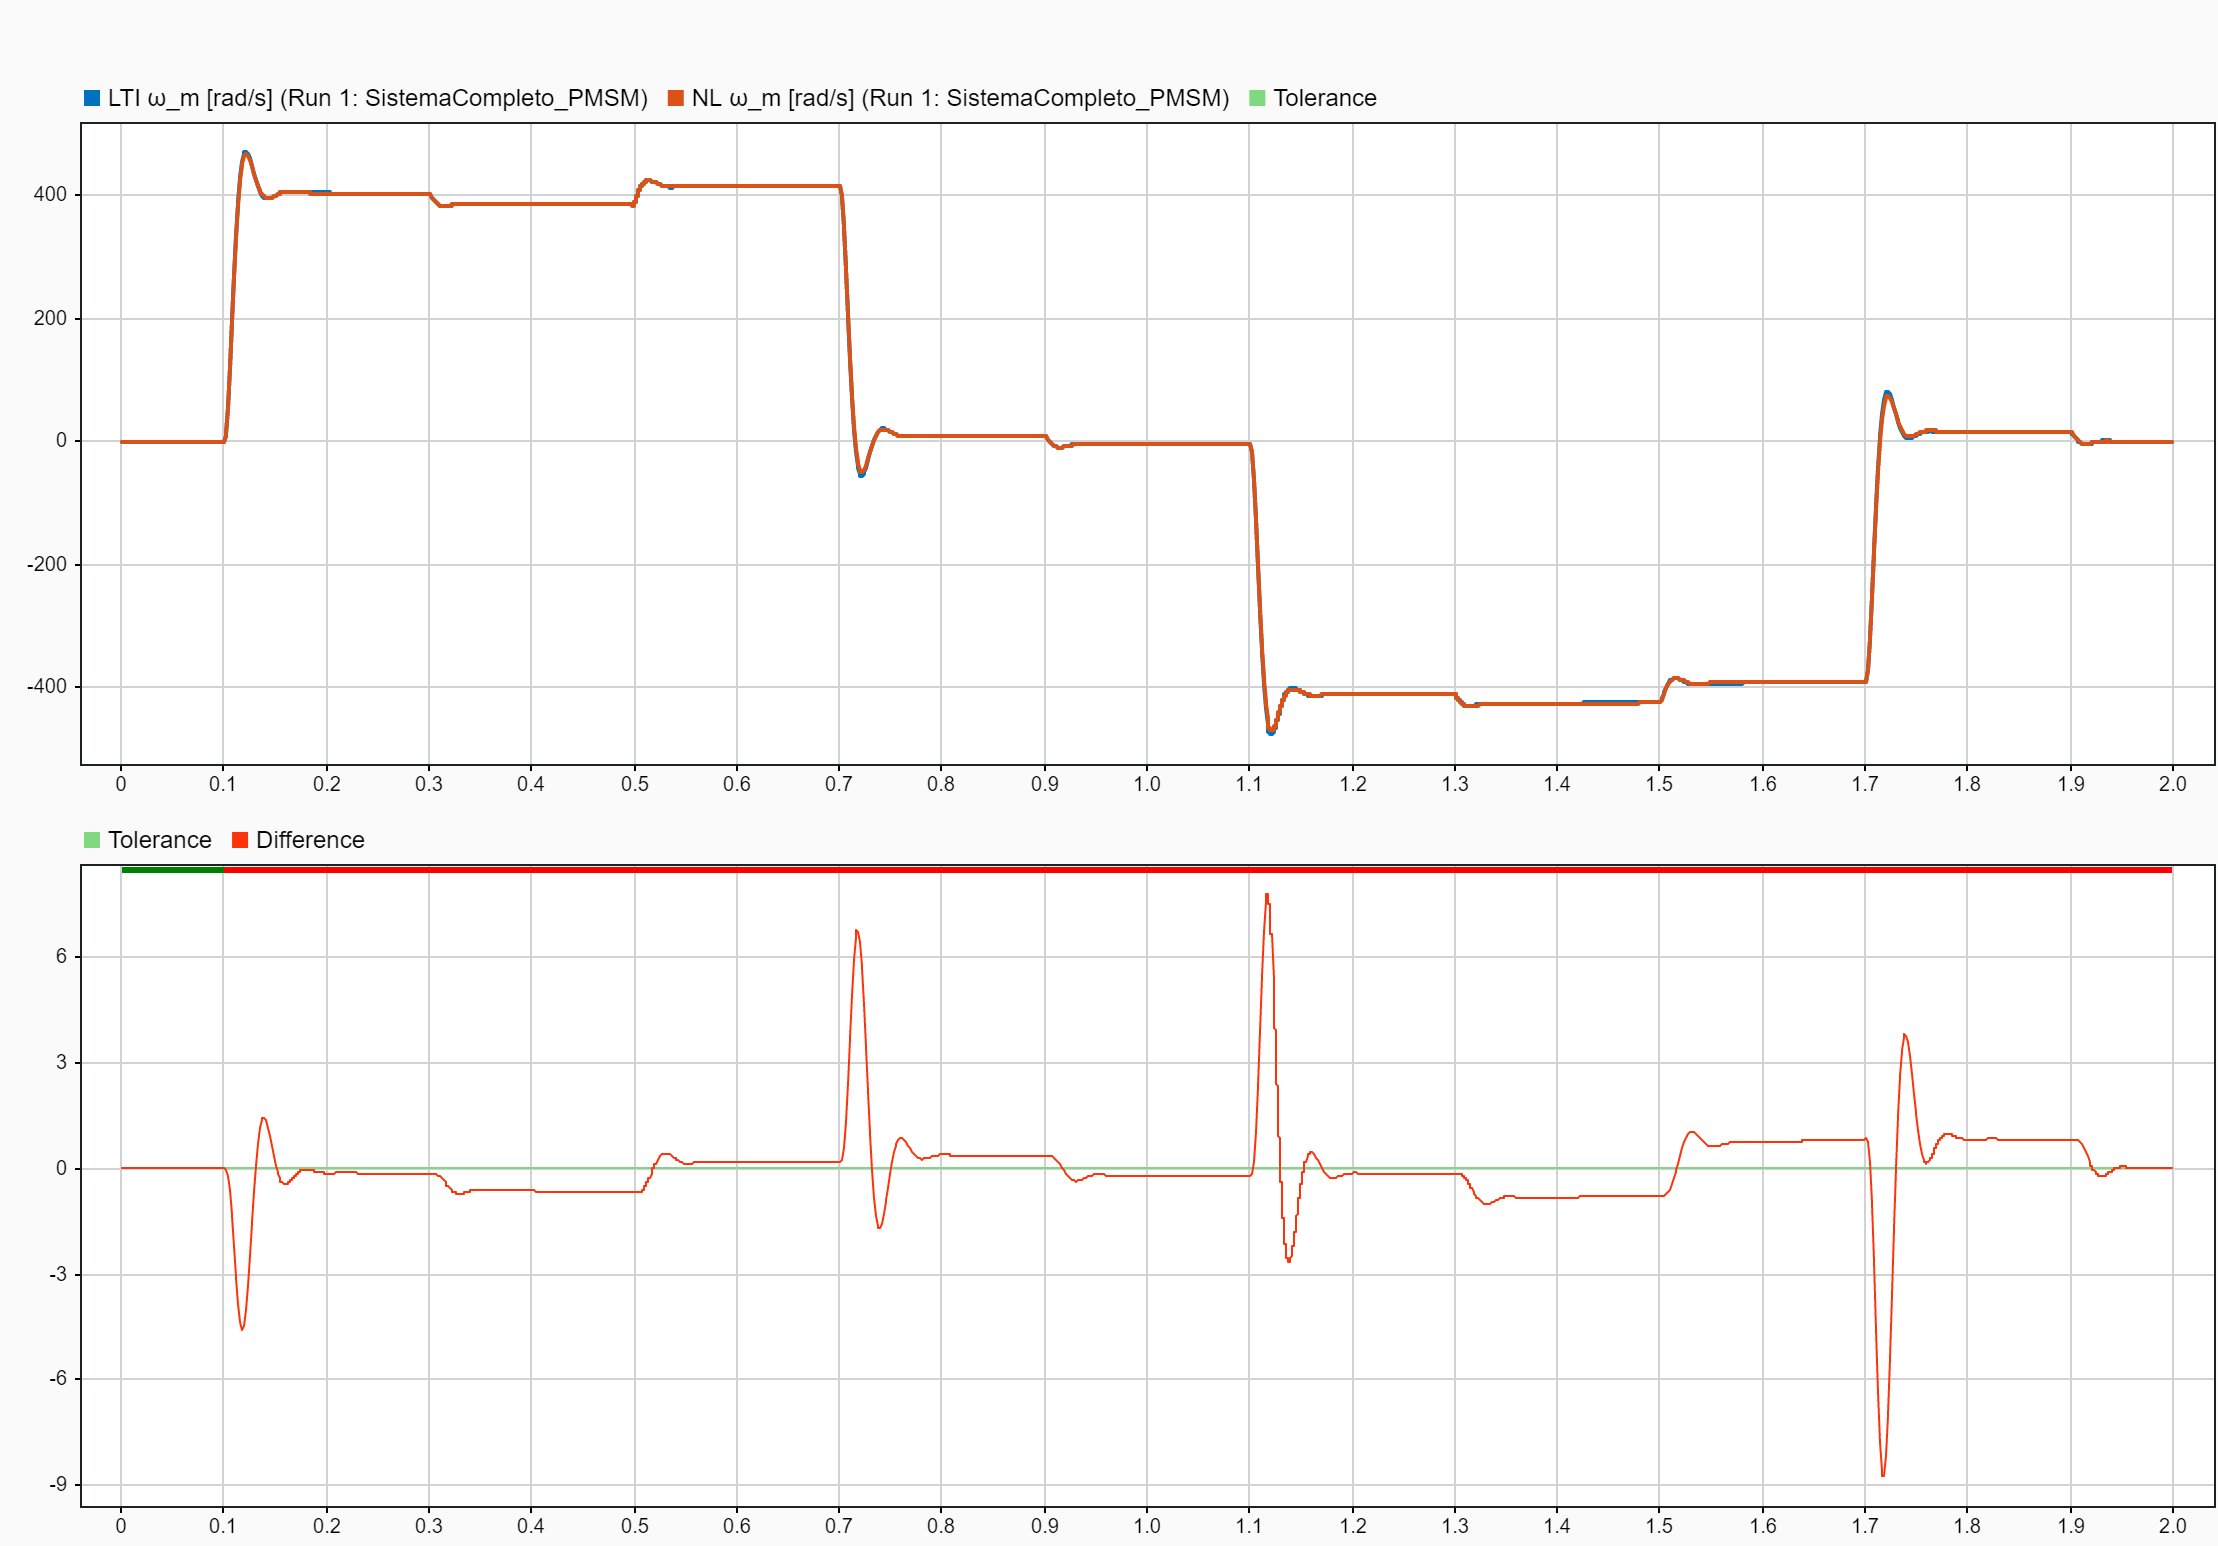
\includegraphics[width=\textwidth]{imagenes/sim_omega_m_error.png}
    \caption{Error de seguimiento en $\omega_m(t)$: diferencia $\omega_m^{\mathrm{NL}}(t)-\omega_m^{\mathrm{LTI}}(t)$, nula en régimen y con picos $\leq 3$~rad/s únicamente en las conmutaciones.}
    \label{fig:sim_omega_m_error}
\end{figure}

\textbf{Corriente $i_{qs}^r(t)$.}

Ante el escalón de $v_{qs}^{r*}$, $i_{qs}^r$ \textbf{no se establece en} $v_{qs}^{r*}/R_{s0}$: es un \textbf{pico de torque transitorio} ($\approx \pm 10{,}4$~A) que decae hasta un valor de régimen pequeño ($\approx 0{,}1$~A) a medida que $\omega_m$ crece y la fuerza contraelectromotriz $\lambda'^r_m P_p \omega_m$ equilibra la tensión (en vacío la corriente solo debe vencer la fricción $b_{eq}\omega_m$). El pico de $\approx \pm 10{,}4$~A es el valor relevante frente a la corriente máxima del motor ($I_{s,max} = 2$~A rms), que este ensayo a lazo abierto supera ampliamente. Ambos modelos se solapan casi perfectamente: el error (Fig.~\ref{fig:sim_iqs_error}) es nulo en régimen y presenta picos $\leq 0{,}1$~A solo en las conmutaciones, confirmando que las leyes de control NL linealizan efectivamente el sistema. Dado que para $i_{ds}^r = 0$ el torque electromagnético se reduce a $T_m = k_t \cdot i_{qs}^r$ (con $k_t = \tfrac{3}{2} P_p \lambda'^r_m$), la forma de onda de $T_m(t)$ es proporcional a $i_{qs}^r(t)$.

\begin{figure}[H]
    \centering
    
\includegraphics[width=\textwidth]{imagenes/sim_iqs.png}
    \caption{Corriente de eje $q$, $i_{qs}^r(t)$: comparación NL (azul) vs LTI aumentado (rojo). Panel inferior: señales de excitación ($T_l$ y $v_{qs}^{r*}$).}
    \label{fig:sim_iqs}
\end{figure}

\begin{figure}[H]
    \centering
    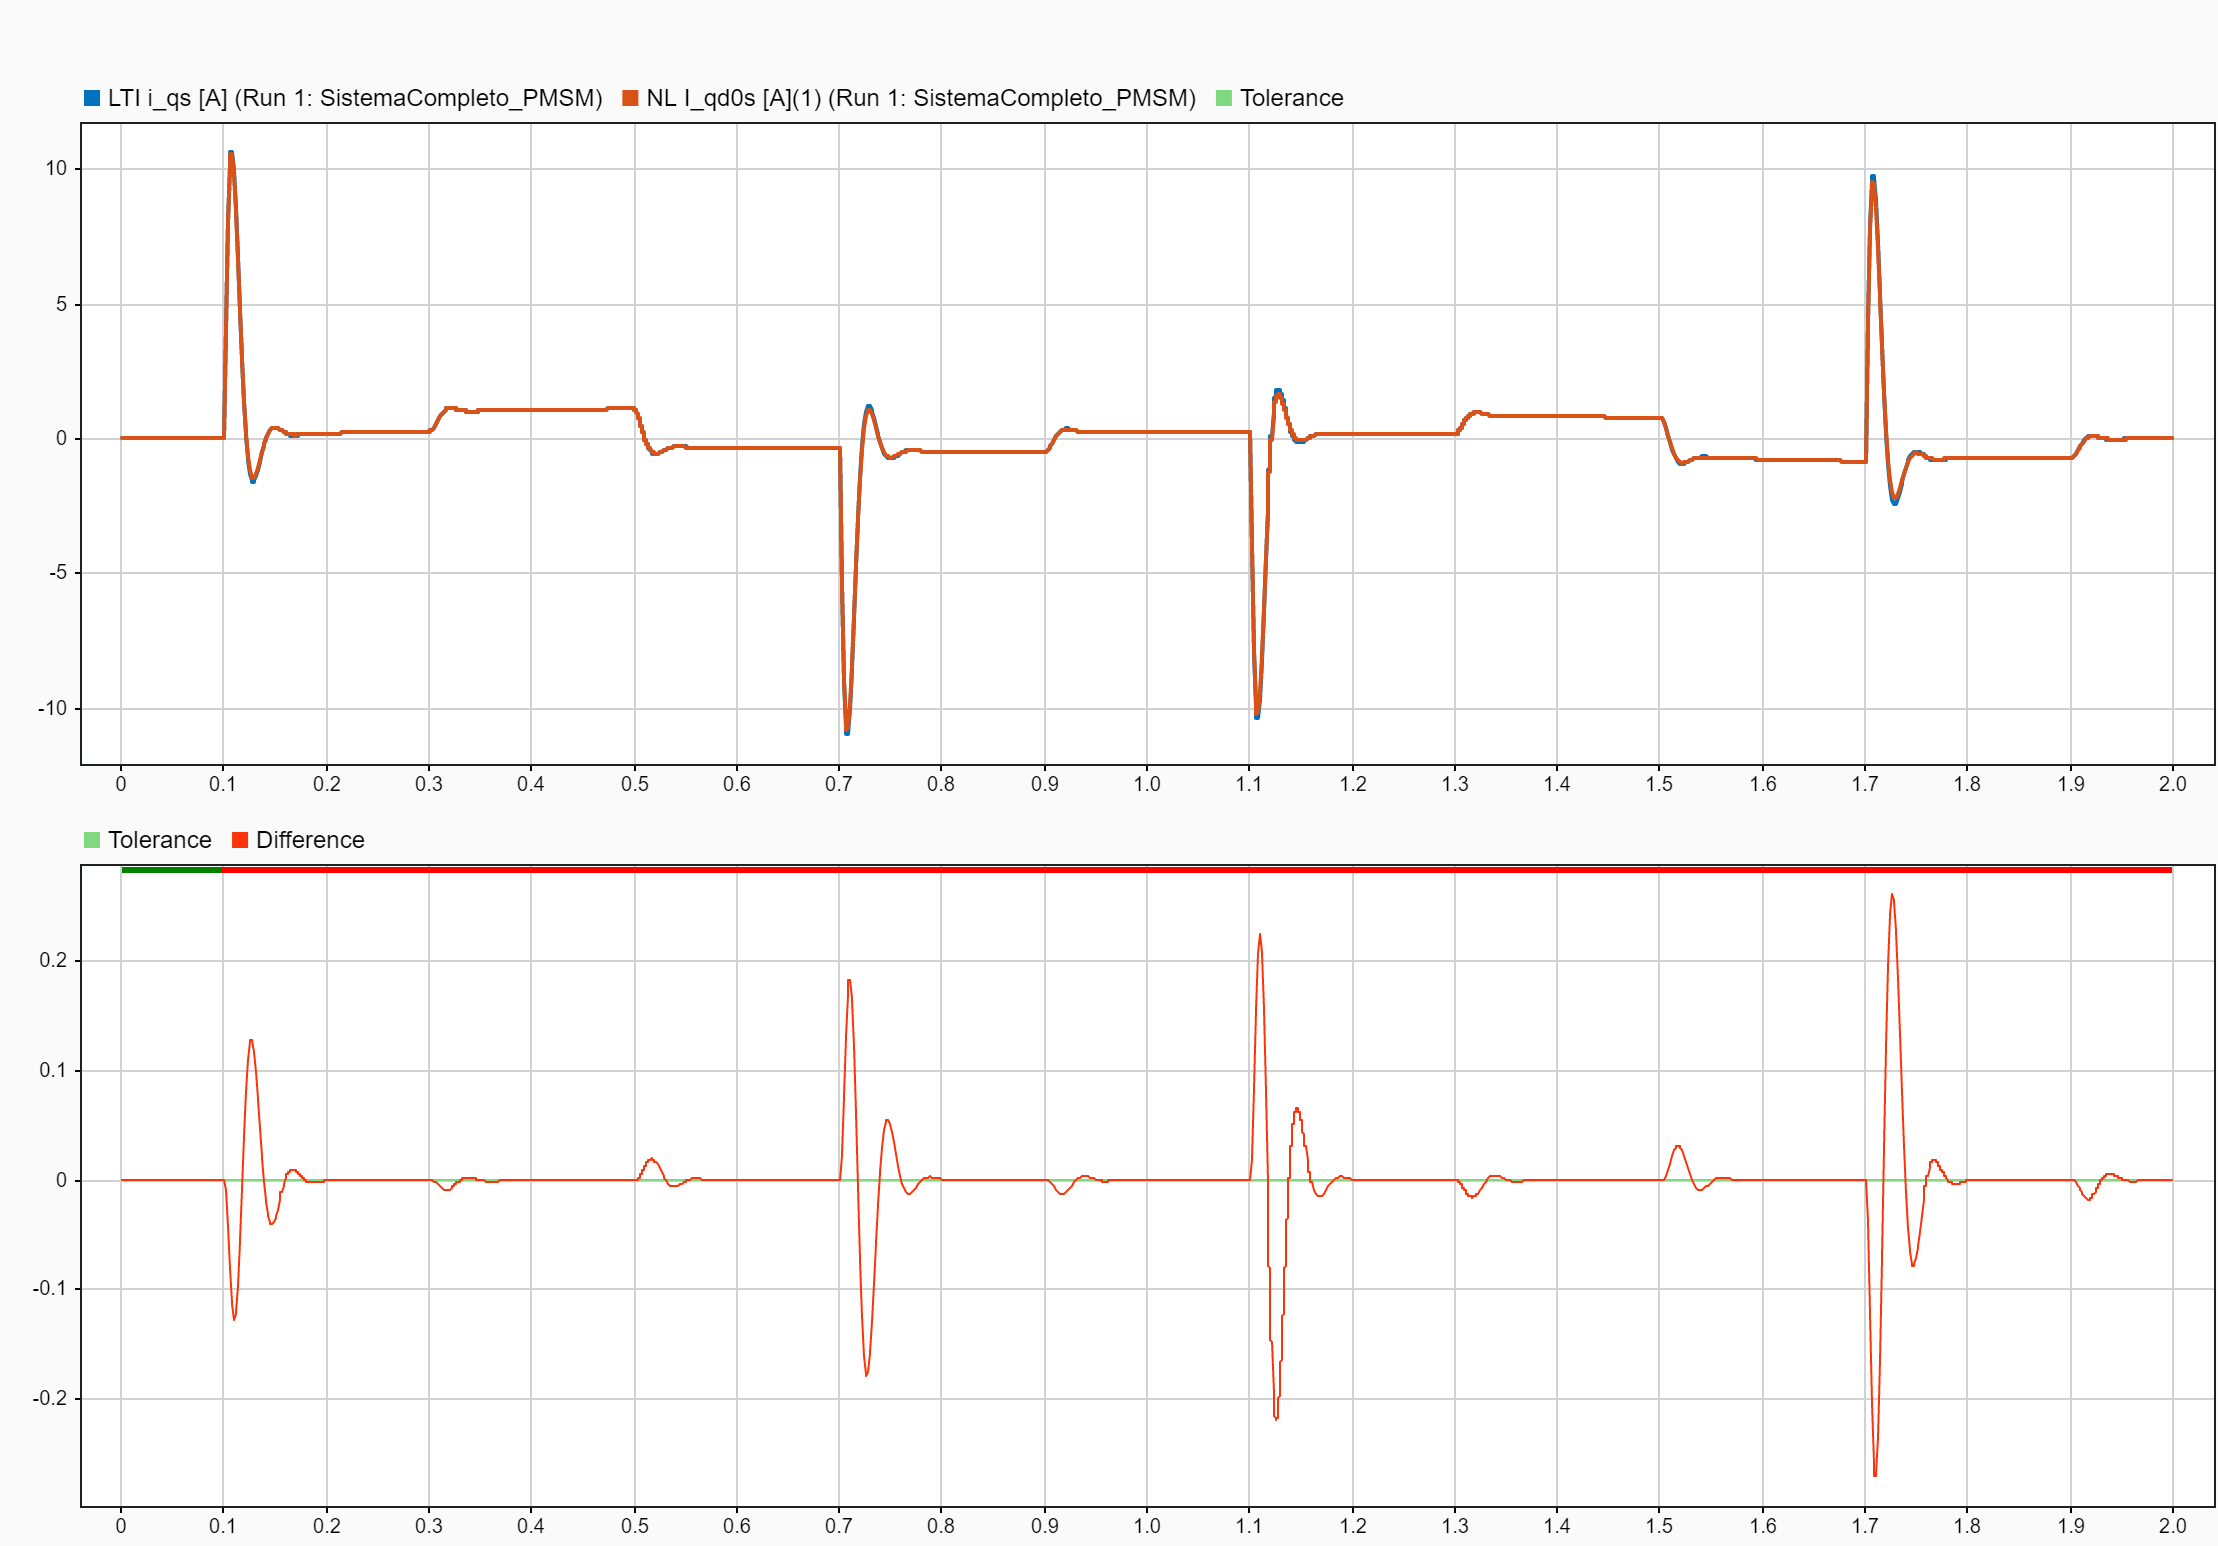
\includegraphics[width=\textwidth]{imagenes/sim_iqs_error.png}
    \caption{Error de seguimiento en $i_{qs}^r(t)$: diferencia $i_{qs}^{r,\mathrm{NL}}(t)-i_{qs}^{r,\mathrm{LTI}}(t)$, nula en régimen y con picos $\leq 0{,}1$~A únicamente en las conmutaciones.}
    \label{fig:sim_iqs_error}
\end{figure}

\textbf{Corrientes $i_{ds}^r(t)$ e $i_{0s}(t)$.}

Para la condición inicial $i_{ds}^r(0) = 0$~A, la corriente de eje $d$ permanece idénticamente nula en ambos modelos durante toda la simulación, ya que no existe excitación externa en el eje $d$ ($v_{ds}^{r*} = 0$) y la ley de control mínima ($v_{ds}^r(t) = -L_q i_{qs}^r(t) \omega_r(t)$) compensa exactamente el acoplamiento cruzado sin inyectar corriente en dicho eje. Análogamente, la corriente de secuencia cero $i_{0s}(t)$ permanece nula al no existir excitación homopolar ($v_{0s}(t) = 0$) ni condición inicial no nula. El comportamiento de $i_{ds}^r(t)$ para condiciones iniciales $i_{ds}^r(0) \neq 0$ se analiza en detalle en el Sub-ítem~c.

\textbf{Temperatura del estator $T_s^\circ(t)$.}

La temperatura crece levemente respecto de $T_{amb}^\circ = 25\,^\circ$C debido a las pérdidas resistivas $P_{s,perd}(t) = \tfrac{3}{2}R_s\big(i_{qs}^{r\,2}(t) + i_{ds}^{r\,2}(t)\big)$. El cambio es mínimo dado que la constante de tiempo térmica $\tau_{th} = R_{ts\text{-}amb} \cdot C_{ts} \approx 120$~s es muy superior a la duración de la simulación ($2{,}2$~s). Este resultado justifica la hipótesis del modelo LTI de utilizar $R_s = R_{s0}$ constante: la variación de resistencia por efecto térmico es despreciable en esta escala temporal. Nótese que el modelo LTI aumentado (4 estados) \textbf{no incluye} la temperatura como variable de estado, ya que asume $R_s$ constante por diseño.

\begin{figure}[H]
    \centering
    
\includegraphics[width=\textwidth]{imagenes/sim_Ts.png}
    \caption{Temperatura del estator $T_s^\circ(t)$ vs t: comparación modelo NL vs LTI aumentado ($i_{ds}^r(0) = 0$~A).}
    \label{fig:sim_Ts}
\end{figure}

\textbf{Tensión $v_{ds}^r(t)$ de la ley de control mínima.}

La ley de control mínima impone internamente la tensión $v_{ds}^r(t) = -L_q \, i_{qs}^r(t) \, \omega_r(t)$, proporcional al producto $i_{qs}^r(t) \cdot \omega_m(t)$. Esta tensión es no nula solo cuando ambas variables lo son simultáneamente, y su magnitud crece con el nivel de operación del sistema.

\begin{figure}[H]
    \centering
    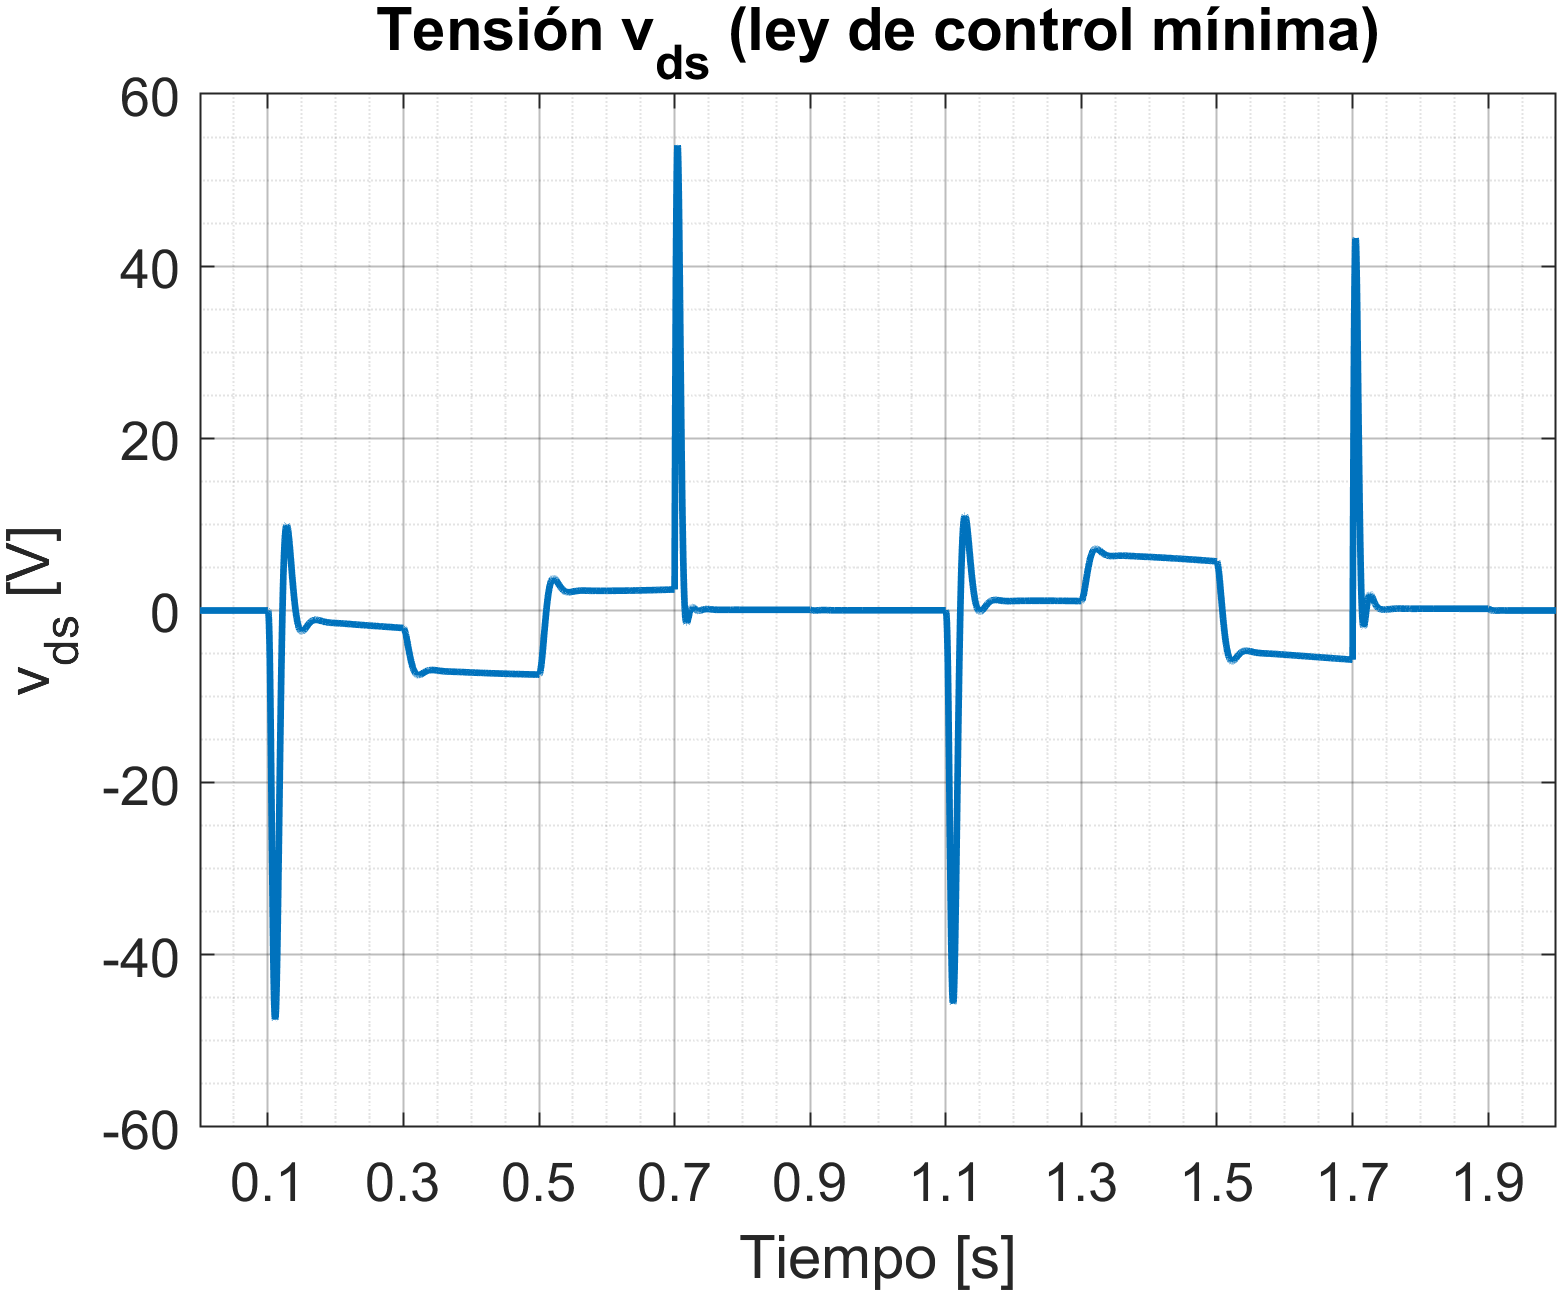
\includegraphics[width=\textwidth]{imagenes/sim_v_ds.png}
    \caption{Tensión $v_{ds}^r(t)$: modelo NL ($i_{ds}^r(0) = 0$~A).}
    \label{fig:sim_v_ds}
\end{figure}

\begin{figure}[H]
    \centering
    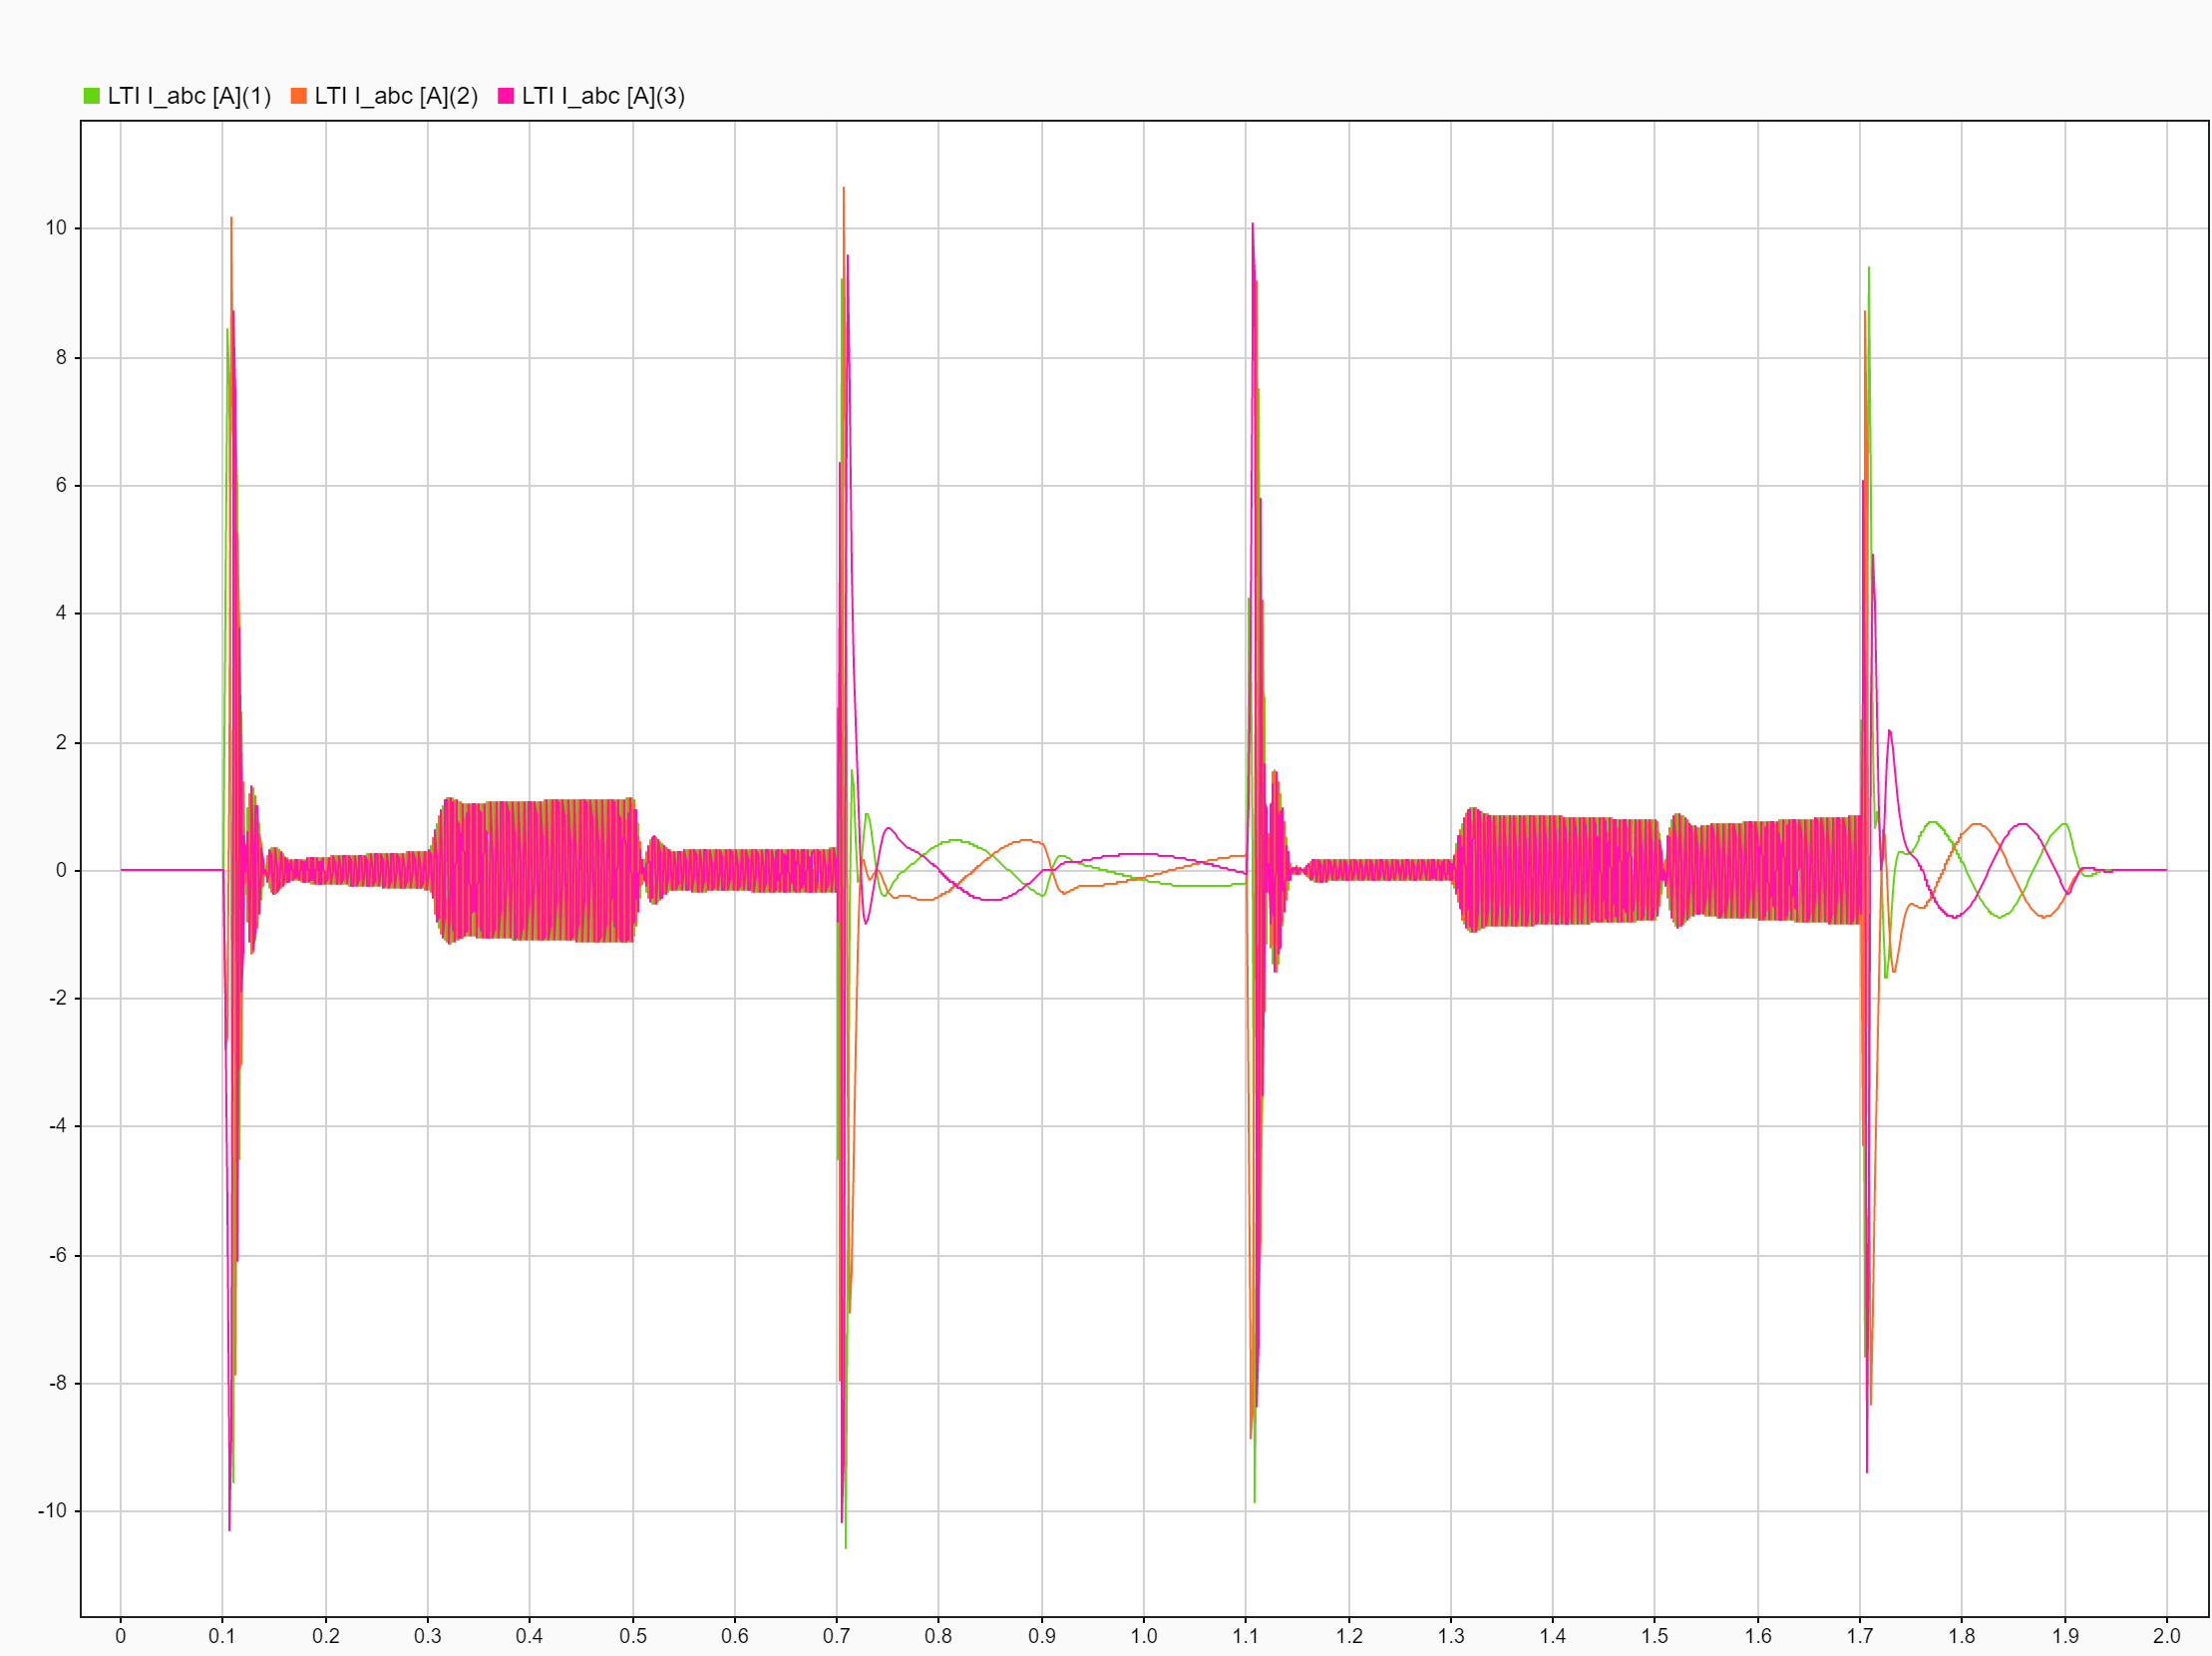
\includegraphics[width=\textwidth]{imagenes/sim_corrientes_abc.png}
    \caption{Corrientes de fase $i_{as}$, $i_{bs}$, $i_{cs}$ obtenidas por Transformación Inversa de Park (modelo NL, $i_{ds}^r(0) = 0$~A).}
    \label{fig:sim_corrientes_abc}
\end{figure}

Las formas de onda resultantes son sinusoidales moduladas en amplitud, con frecuencia eléctrica $\omega_r = P_p \cdot \omega_m$ proporcional a la velocidad del rotor. Cuando $\omega_m = 0$ (antes de $t = 0{,}1$~s y en los intervalos de velocidad nula), las corrientes $abc$ son constantes (frecuencia eléctrica nula). A medida que el motor acelera, la frecuencia de las oscilaciones crece proporcionalmente.

Mediante la misma Transformación Inversa de Park se obtienen las tensiones de fase aplicadas al estator por el inversor. La Fig.~\ref{fig:sim_tensiones_abc} las presenta, respetando el mismo código de colores por fase utilizado en las corrientes.

\begin{figure}[H]
    \centering
    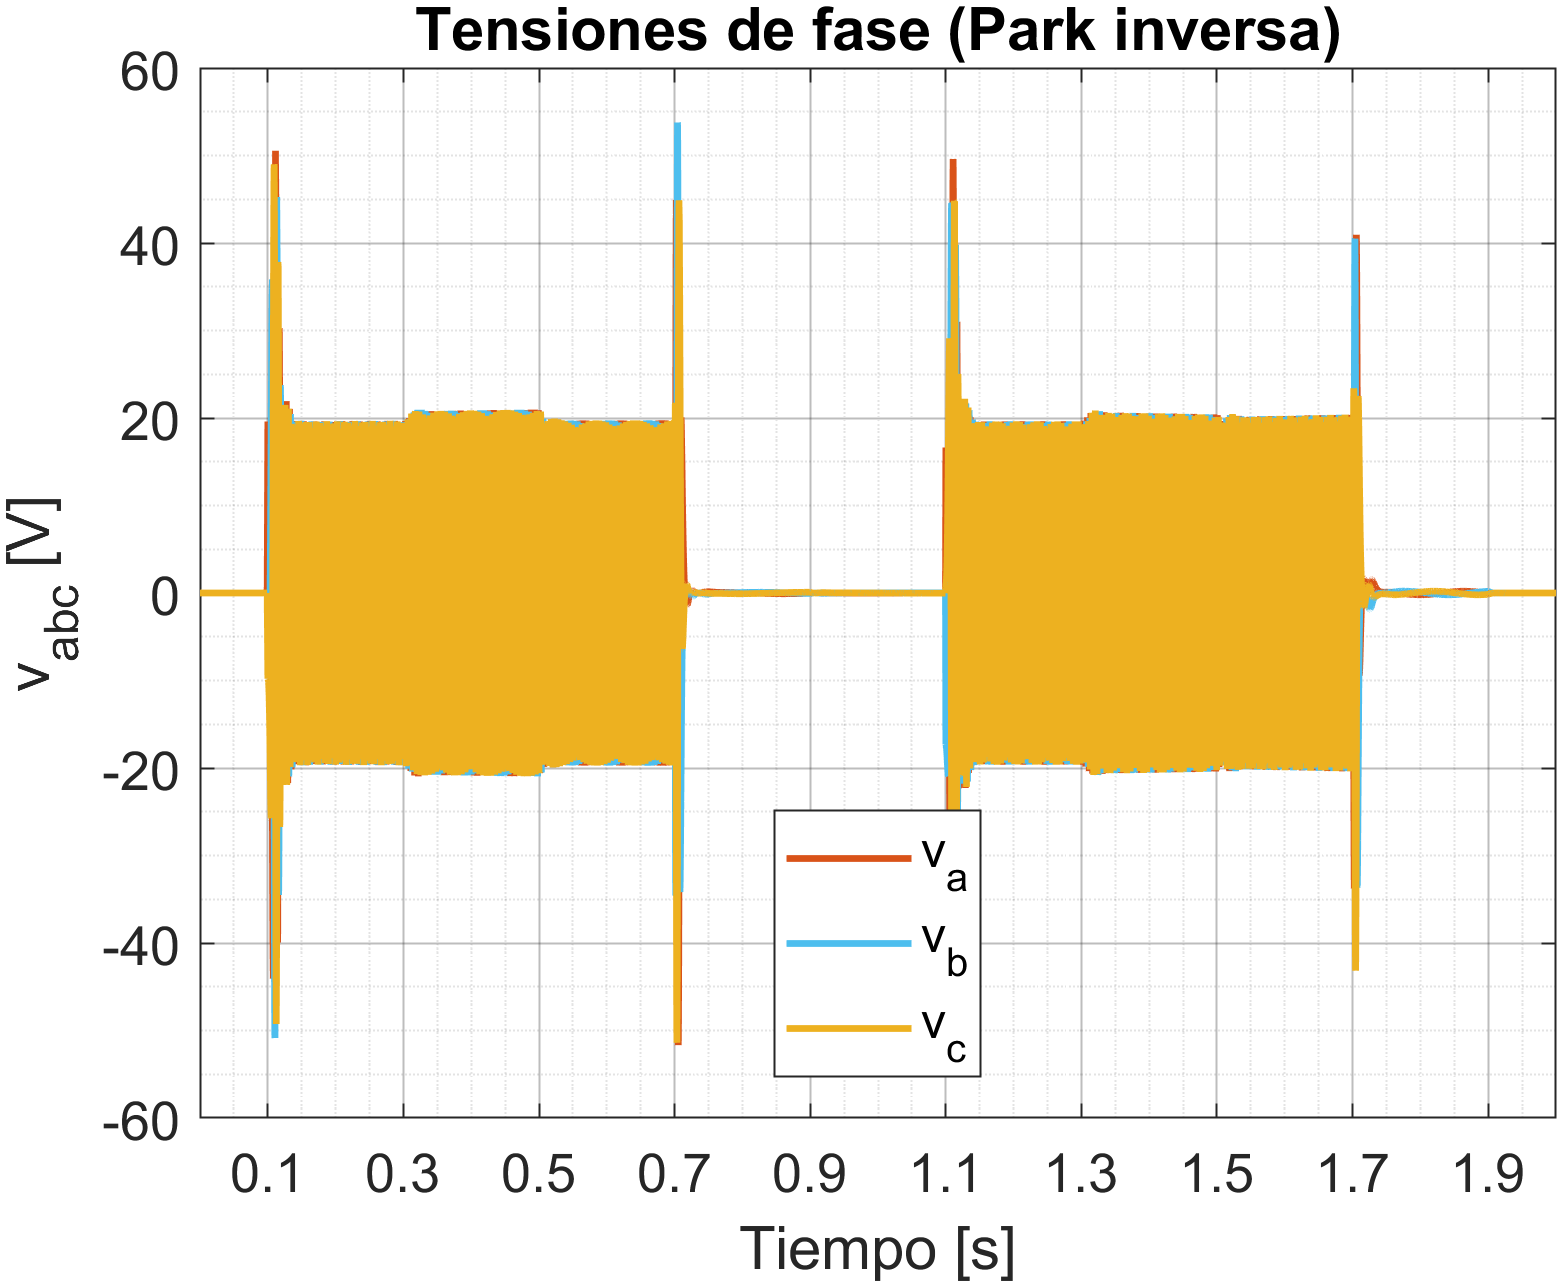
\includegraphics[width=\textwidth]{imagenes/sim_tensiones_abc.png}
    \caption{Tensiones de fase $v_{as}$, $v_{bs}$, $v_{cs}$ aplicadas al estator (modelo NL, $i_{ds}^r(0)=0$~A), con el mismo código de colores por fase que las corrientes.}
    \label{fig:sim_tensiones_abc}
\end{figure}

\textbf{Curva paramétrica: torque vs velocidad (cuadrantes de operación).}

La curva paramétrica $T_m(\omega_m)$ se construye a partir de los datos del script MATLAB, segmentando la trayectoria en 10 transitorios que conectan los puntos de (cuasi-)equilibrio $P_0$ a $P_{10}$.

\begin{figure}[H]
    \centering
    
\includegraphics[width=\textwidth]{imagenes/sim_torque_vs_velocidad.png}
    \caption{Torque electromagnético vs velocidad angular: cuadrantes de operación del motor PMSM. Cada transitorio se distingue por color, con flechas indicando el sentido de recorrido y diamantes marcando los puntos de equilibrio $P_0$ a $P_{10}$.}
    \label{fig:sim_torque_vel}
\end{figure}

El sistema recorre los cuatro cuadrantes durante la secuencia completa de pulsos:
\begin{itemize}
    \item \textbf{Cuadrante I} ($+\omega_m, +T_m$): motorización en sentido positivo. El motor entrega torque en el mismo sentido que la velocidad.
    \item \textbf{Cuadrante II} ($-\omega_m, +T_m$): frenado regenerativo en sentido negativo.
    \item \textbf{Cuadrante III} ($-\omega_m, -T_m$): motorización en sentido negativo, análogo al Cuadrante~I para el pulso negativo de $v_{qs}^{r*}$.
    \item \textbf{Cuadrante IV} ($+\omega_m, -T_m$): frenado regenerativo en sentido positivo. El torque frena la velocidad positiva residual.
\end{itemize}


\textbf{Ángulo de Carga $\delta(t)$}

El ángulo de carga $\delta(t)$ representa el desfasaje electromagnético entre el ángulo eléctrico $\theta_{ev}(t)$ y la posición angular del rotor en coordenadas eléctricas $\theta_r(t)$. Como referencia eléctrica se utiliza la posición de la tensión $v_{as}(t)$, que es constante en estado estacionario.
\begin{equation}\label{eq:angulo_carga}
    \delta(t) \equiv \theta_{ev}(t)-\theta_r(t) = \int_0^t[\omega_e(\xi)-\omega_r(\xi)]d\xi +[\theta_{ev}(0)-\theta_r(0)]
\end{equation}
Tal que:
\begin{itemize}
    \item $\omega_e$: velocidad angular de la referencia (tensión de fase \textbf{a}).
    \item $\omega_r$: velocidad angular del rotor.
\end{itemize}
Al mismo tiempo, se asumen posiciones angulares iniciales nulas para ambas variables.\\
\textbf{Cálculo de la coordenada eléctrica sincrónica $\theta_{ev}$:}
\begin{align*}
v_{as}(t) &\approx \sqrt{2}\,\frac{V_{sl}(t)}{\sqrt{3}} \cos\big(\theta_{ev}(t)\big) \\
v_{bs}(t) &\approx \sqrt{2}\,\frac{V_{sl}(t)}{\sqrt{3}} \cos\left(\theta_{ev}(t) - \frac{2\pi}{3}\right) \\
v_{cs}(t) &\approx \sqrt{2}\,\frac{V_{sl}(t)}{\sqrt{3}} \cos\left(\theta_{ev}(t) + \frac{2\pi}{3}\right)
\end{align*}
Siendo $\sqrt{2}\,V_{sl}/\sqrt{3}$ el valor pico de la tensión de fase aplicada, con $V_{sl}$ el módulo de la tensión de línea (notación de la guía).
Es necesario aplicar la Transformación de Clarke para proyectar las tensiones sobre un plano:
\begin{align*}
    v_{\alpha}(t) = \frac{2}{3}\Big(v_{as}(t) - \frac{1}{2}v_{bs}(t)-\frac{1}{2}v_{cs}(t)\Big) \\
    v_{\beta}(t) = \frac{\sqrt{3}}{3}\big(v_{bs}(t)-v_{cs}(t)\big)
\end{align*}
Sustituyendo, se obtiene:
\begin{align}
    v_{\alpha}(t) = \sqrt{2}\,\tfrac{V_{sl}(t)}{\sqrt{3}} \cos{\theta_{ev}(t)} \\
    v_{\beta}(t) = \sqrt{2}\,\tfrac{V_{sl}(t)}{\sqrt{3}} \sin{\theta_{ev}(t)}
\end{align}
Por lo tanto, para obtener el ángulo $\theta_{ev}$ basta con aplicar la función \textit{atan2} tal que:
\begin{equation}
    \theta_{ev}(t) = \text{atan2}\big(v_{\beta}(t),v_{\alpha}(t)\big)= \text{atan2}\big(\sqrt{2}\,\tfrac{V_{sl}(t)}{\sqrt{3}} \sin{\theta_{ev}(t)},\ \sqrt{2}\,\tfrac{V_{sl}(t)}{\sqrt{3}} \cos{\theta_{ev}(t)}\big)
\end{equation}

\begin{figure}[H]
    \centering
    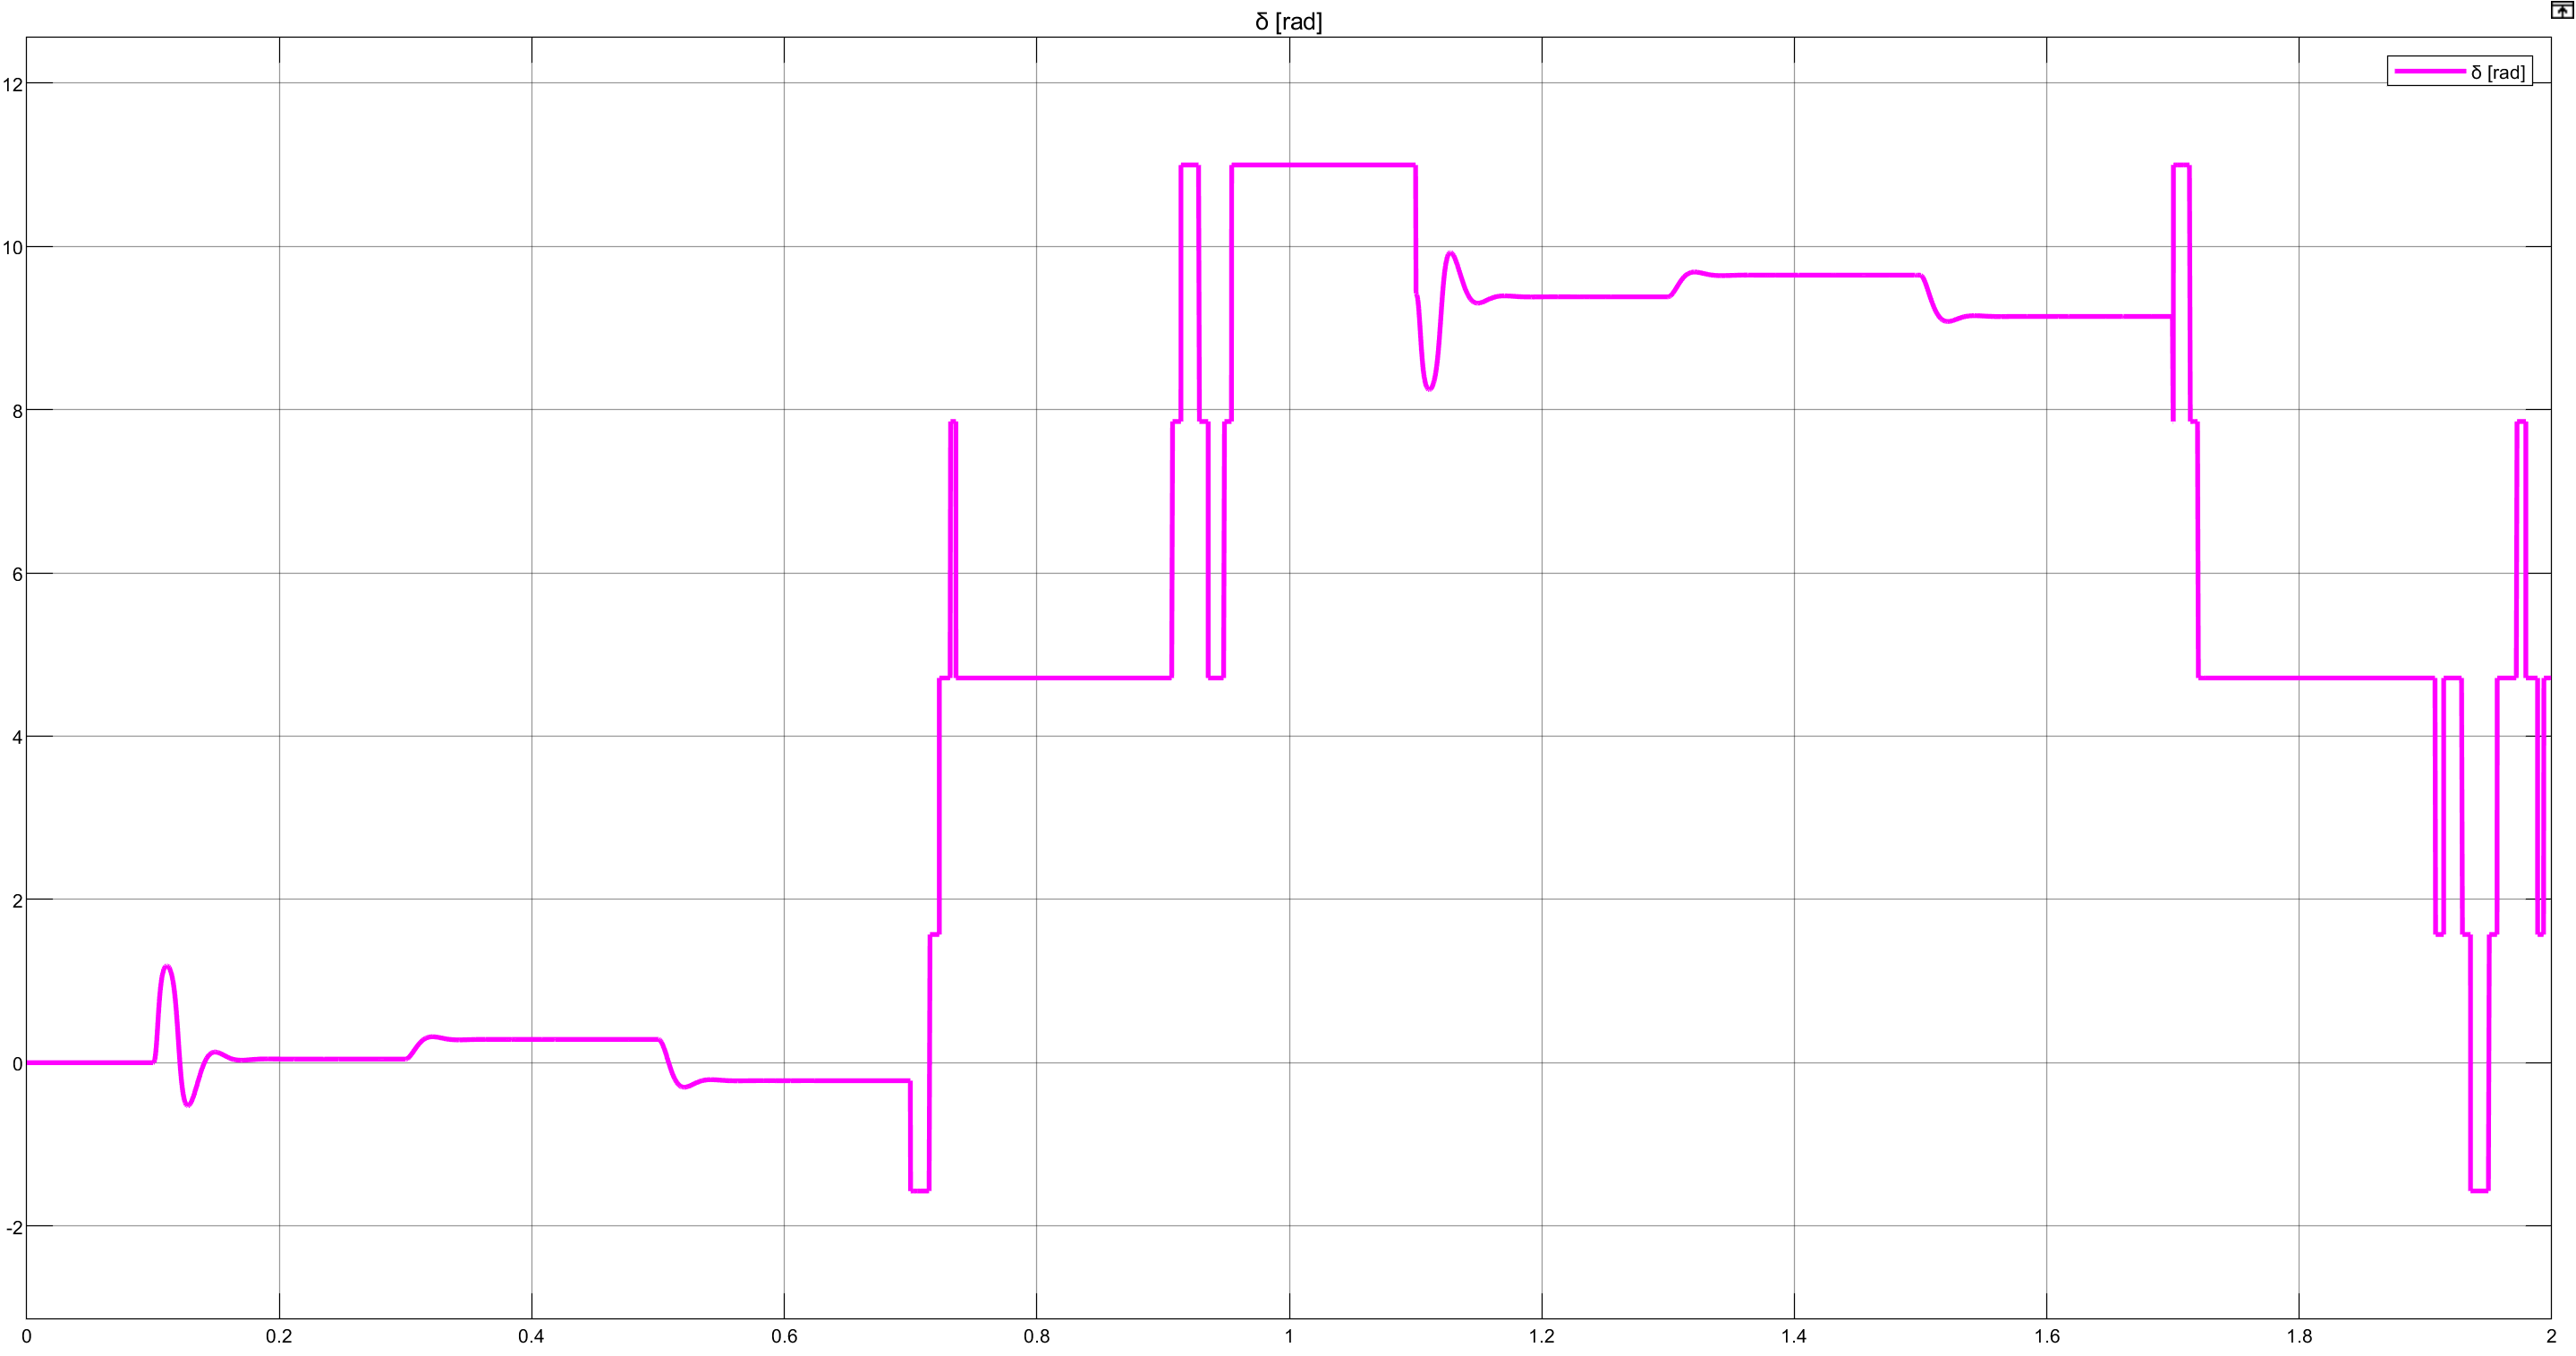
\includegraphics[width=\textwidth]{imagenes/sim_angulo_carga.png}
    \caption{Ángulo de carga $\delta(t)$ vs t (modelo NL, $i_{ds}^r(0) = 0$~A).}
    \label{fig:sim_angulo_carga}
\end{figure}
% =====================================================================
\subsubsection{Métricas de transitorio (Sub-ítem b)}
\label{sec:sim_item_b}

Se determinan las métricas de los 10 transitorios para el caso nominal $i_{ds}^r(0) = 0$~A del modelo LTI aumentado. Dado que la variable subamortiguada es la \textbf{velocidad} $\omega_m$ (gobernada por el par de polos complejos $\zeta = 0{,}527$, $\omega_n = 174$~rad/s), las métricas de sobrepico $M_p$, tiempo de pico $t_p$, tiempo de crecimiento 10--90\% $t_r$ y tiempo de establecimiento $\pm 1\%$ $t_s$ se miden \textbf{sobre $\omega_m$}. Se reporta además el valor de régimen $\omega_{m,ss}$ y, para la corriente, sus valores pico y de régimen (la corriente es un pico de torque que decae, no un escalón de primer orden). La Tabla~\ref{tab:metricas_trans} resume los resultados extraídos de la simulación.

Gracias al acoplamiento electromagnético, $\omega_m$ \textbf{sí alcanza} su valor de régimen dentro de cada segmento de 200~ms ($t_s \approx 50$~ms $\ll 0{,}2$~s), con el sobrepico característico de $\zeta = 0{,}527$. No rige aquí la lenta constante mecánica $\tau_m = J_{eq}/b_{eq} = 0{,}90$~s, que correspondería al subsistema mecánico desacoplado de la realimentación de fuerza contraelectromotriz.

\begin{table}[H]
    \centering
    \caption{Métricas de transitorio para cada evento de conmutación (modelo LTI aumentado, $i_{ds}^r(0) = 0$~A). $M_p$, $t_p$, $t_r$ y $t_s$ medidos sobre $\omega_m$.}
    \label{tab:metricas_trans}
    \renewcommand{\arraystretch}{1.15}
    \scriptsize
    \begin{tabular}{|c|l|r|r|r|r|r|r|r|}
        \hline
        \textbf{Tr.} & \textbf{Evento} & $\omega_{m,ss}$ & $M_p$ & $t_p$ & $t_r$ & $t_s$ & $i_{qs,\mathrm{pico}}^r$ & $i_{qs,ss}^r$ \\
         & & [rad/s] & [\%] & [ms] & [ms] & [ms] & [A] & [A] \\
        \hline
        1  & $v_{qs}^{r*} \to +19{,}6$~V & $405{,}5$ & $14{,}3$ & $21{,}3$ & $9{,}7$ & $50{,}1$ & $10{,}39$ & $0{,}12$ \\
        2  & $T_{ld} \to +6{,}28$~Nm & $389{,}6$ & $25{,}6$ & $14{,}4$ & $5{,}8$ & $45{,}7$ & $0{,}95$ & $0{,}85$ \\
        3  & $T_{ld} \to -6{,}28$~Nm & $421{,}4$ & $25{,}6$ & $14{,}3$ & $5{,}8$ & $45{,}7$ & $0{,}85$ & $-0{,}60$ \\
        4  & $v_{qs}^{r*} \to 0$~V & $15{,}9$ & $14{,}3$ & $21{,}3$ & $9{,}7$ & $50{,}1$ & $-10{,}99$ & $-0{,}72$ \\
        5  & $T_{ld} \to 0$~Nm & $0{,}0$ & $25{,}6$ & $14{,}3$ & $5{,}8$ & $45{,}7$ & $-0{,}72$ & $0{,}00$ \\
        6  & $v_{qs}^{r*} \to -19{,}6$~V & $-405{,}5$ & $14{,}3$ & $21{,}2$ & $9{,}7$ & $50{,}1$ & $-10{,}39$ & $-0{,}12$ \\
        7  & $T_{ld} \to +6{,}28$~Nm & $-421{,}4$ & $25{,}6$ & $14{,}4$ & $5{,}8$ & $45{,}7$ & $0{,}70$ & $0{,}60$ \\
        8  & $T_{ld} \to -6{,}28$~Nm & $-389{,}6$ & $25{,}6$ & $14{,}4$ & $5{,}8$ & $45{,}7$ & $-1{,}05$ & $-0{,}85$ \\
        9  & $v_{qs}^{r*} \to 0$~V & $15{,}9$ & $14{,}3$ & $21{,}3$ & $9{,}7$ & $50{,}1$ & $9{,}55$ & $-0{,}72$ \\
        10 & $T_{ld} \to 0$~Nm & $0{,}0$ & $25{,}6$ & $14{,}4$ & $5{,}8$ & $45{,}7$ & $-0{,}72$ & $0{,}00$ \\
        \hline
    \end{tabular}

    \vspace{2mm}
    \scriptsize $\omega_{m,ss}$: velocidad de régimen del segmento. $M_p$, $t_p$ (pico), $t_r$ (10--90\%) y $t_s$ ($\pm1\%$): métricas sobre $\omega_m$. $i_{qs,\mathrm{pico}}^r$/$i_{qs,ss}^r$: valor pico y de régimen de la corriente de eje $q$.
\end{table}

\textbf{Observaciones:}
\begin{itemize}
    \item Ante los escalones de $v_{qs}^{r*}$ (transitorios 1, 4, 6, 9), $\omega_m$ alcanza la velocidad de vacío ($\approx \pm 405$~rad/s) con un \textbf{sobrepico de $\approx 14{,}3\%$}, tiempo de pico $\approx 21$~ms y establecimiento ($\pm 1\%$) $\approx 50$~ms, consistentes con el par de polos complejos $\zeta = 0{,}527$, $\omega_n = 174$~rad/s. La corriente $i_{qs}^r$ \textbf{no} se establece en $v_{qs}^{r*}/R_{s0}$: es un \textbf{pico de torque} ($\approx \pm 10{,}4$~A) que decae a $\approx 0{,}1$~A al crecer la velocidad y aparecer la fuerza contraelectromotriz.

    \item Los eventos de $T_{ld}$ producen una excursión de velocidad menor (de $\pm 16$ a $\pm 32$~rad/s respecto del valor previo) con el mismo modo subamortiguado, y \textbf{sí modifican} $i_{qs}^r$ en régimen ($\approx \pm 0{,}6$--$0{,}85$~A por cada $6{,}28$~Nm): la corriente de operación debe suministrar el torque de carga referido $T_{ld}/r$. Es decir, en este modelo a lazo abierto los ejes \textbf{no} están completamente desacoplados.
\end{itemize}

\textbf{Influencia relativa de las acciones externas:}

\begin{itemize}
    \item \textbf{Tensión $v_{qs}^{r*}(t)$}: es la acción \textbf{dominante}. Fija la velocidad de vacío del motor (donde la fuerza contraelectromotriz equilibra la tensión aplicada) y produce el pico de corriente/torque ($\approx \pm 10{,}4$~A); la respuesta de $\omega_m$ es subamortiguada (sobrepico $\approx 14\%$).

    \item \textbf{Torque de carga $T_{ld}(t)$}: perturba la velocidad (excursión moderada) y desplaza el punto de operación de la corriente. No introduce una escala temporal distinta: excita el mismo modo electromecánico complejo.

    \item A diferencia de una lectura desacoplada, el sistema \textbf{no} exhibe dos escalas separadas (eléctrica $\tau_e$ y mecánica $\tau_m$): la realimentación de fuerza contraelectromotriz fusiona ambas en una \textbf{resonancia electromecánica subamortiguada} ($\zeta = 0{,}527$, $\omega_n = 174$~rad/s, $\tau \approx 11$~ms), que se observa tanto en $\omega_m$ como en $i_{qs}^r$.
\end{itemize}

% =====================================================================
\subsubsection{Efecto de $i_{ds}^r(0)$ sobre el sistema (Sub-ítem c)}
\label{sec:sim_item_c}

Se compara el comportamiento de $i_{ds}^r(t)$ para las tres condiciones iniciales en ambos modelos.

\begin{figure}[H]
    \centering
    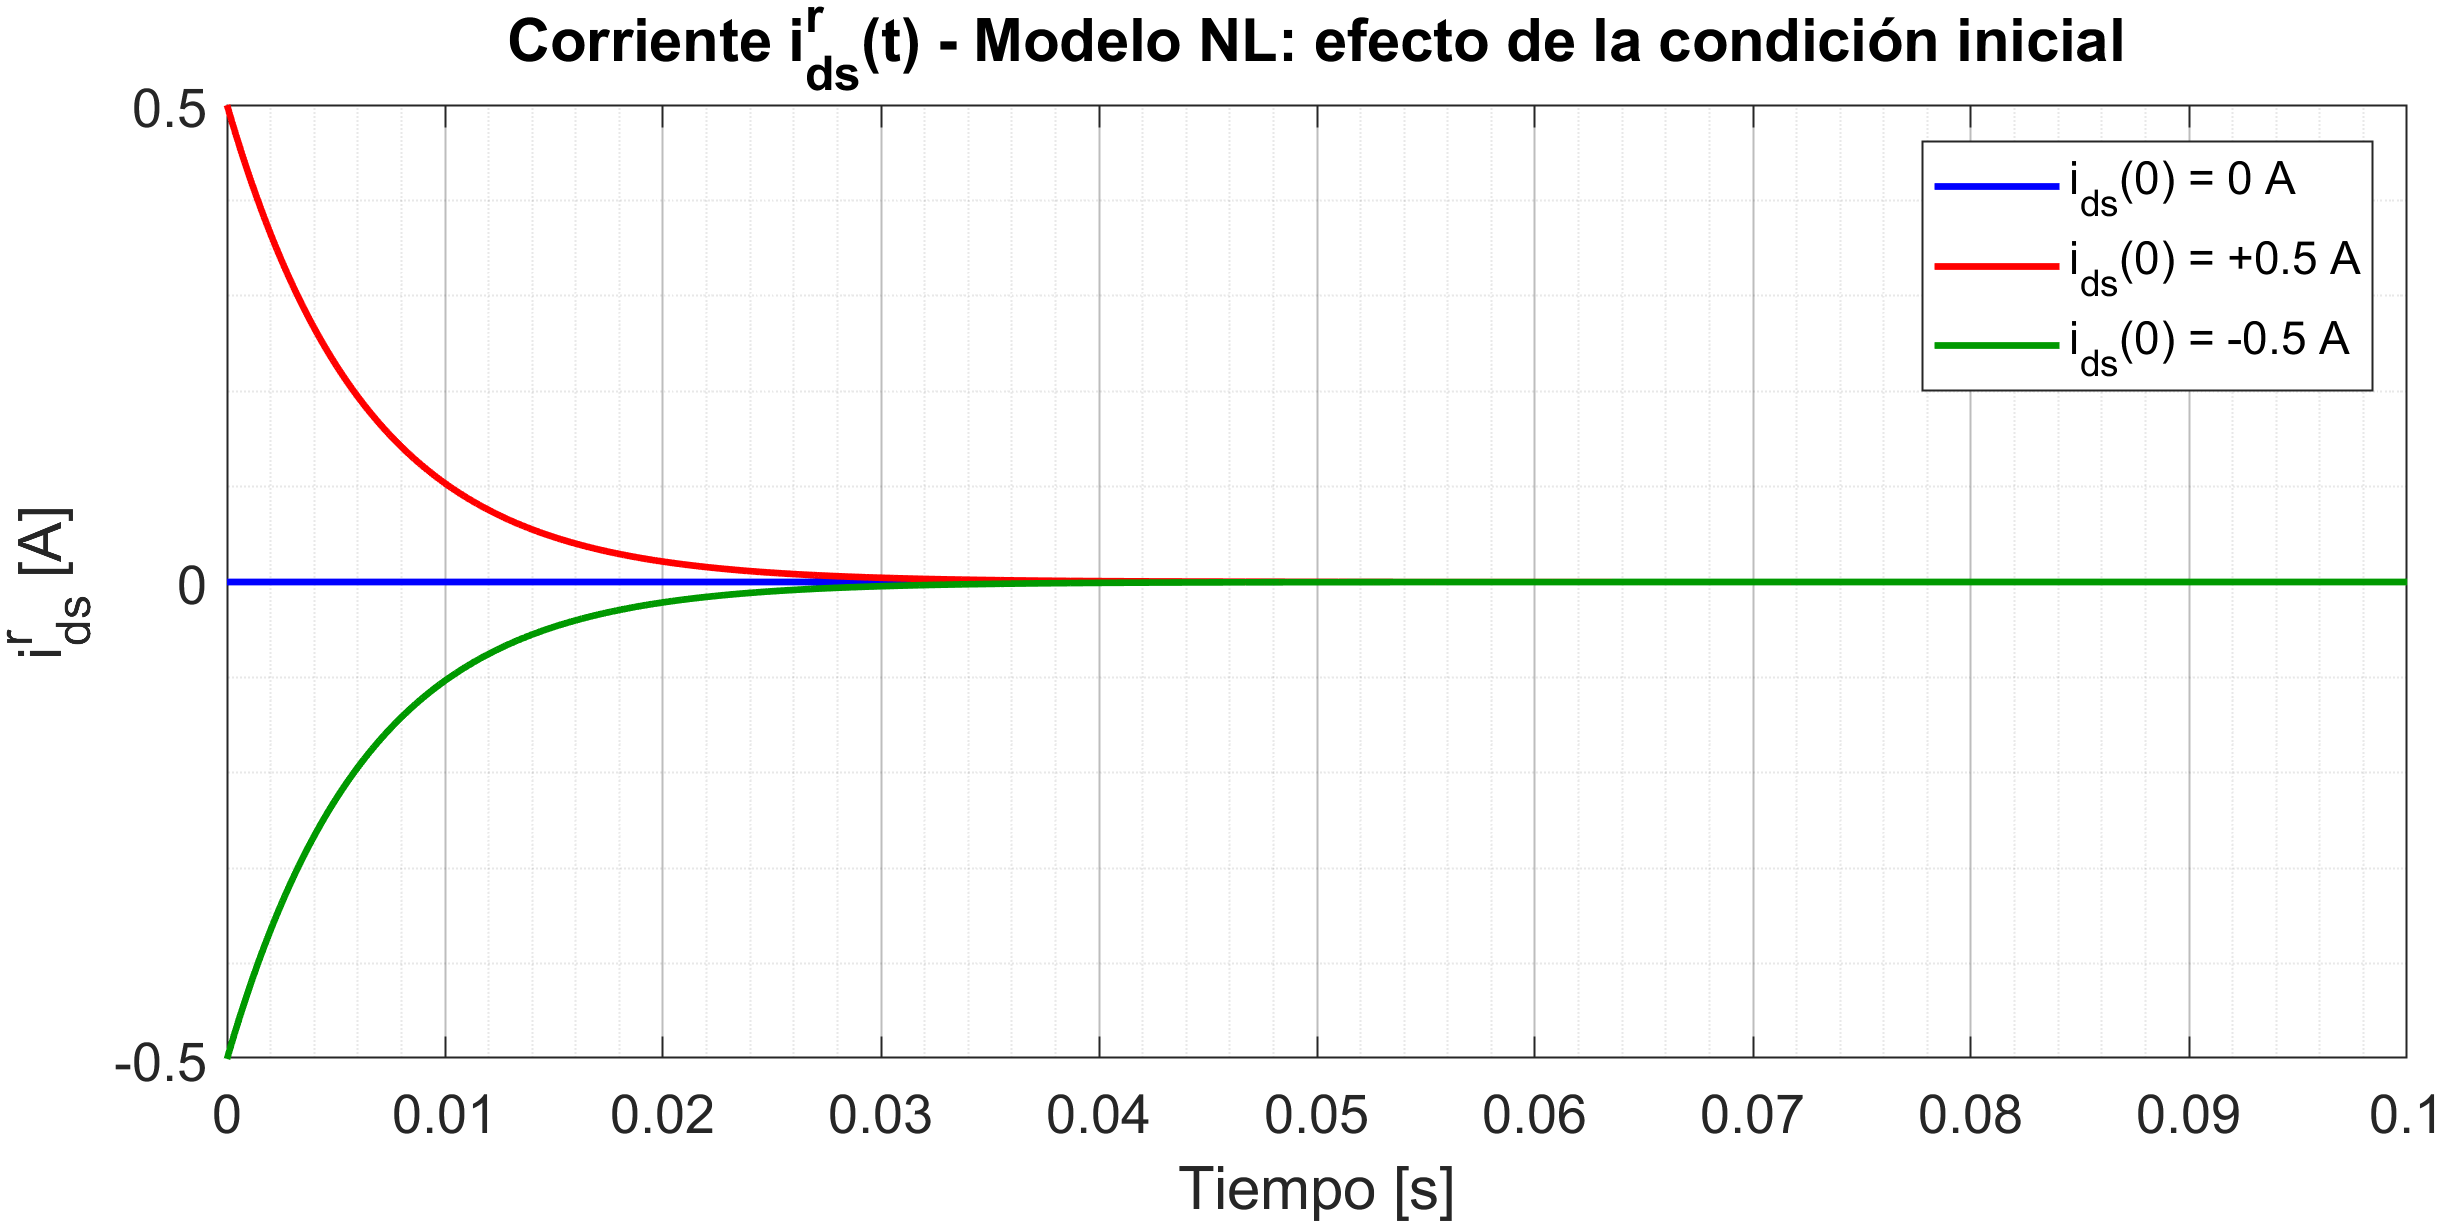
\includegraphics[width=0.9\textwidth]{imagenes/sim_ids_NL_3casos.png}
    \caption{Comparación de $i_{ds}^r(t)$ para $i_{ds}^r(0) \in \{0,\; +0{,}5,\; -0{,}5\}$~A: modelo NL.}
    \label{fig:sim_comparacion_ids}
\end{figure}

\begin{figure}[H]
    \centering
    
\includegraphics[width=0.9\textwidth]{imagenes/sim_ids_LTI_3casos.png}
    \caption{Comparación de $i_{ds}^r(t)$ para $i_{ds}^r(0) \in \{0,\; +0{,}5,\; -0{,}5\}$~A: modelo LTI.}
    \label{fig:sim_ids_zoom}
\end{figure}

\begin{figure}[H]
    \centering
    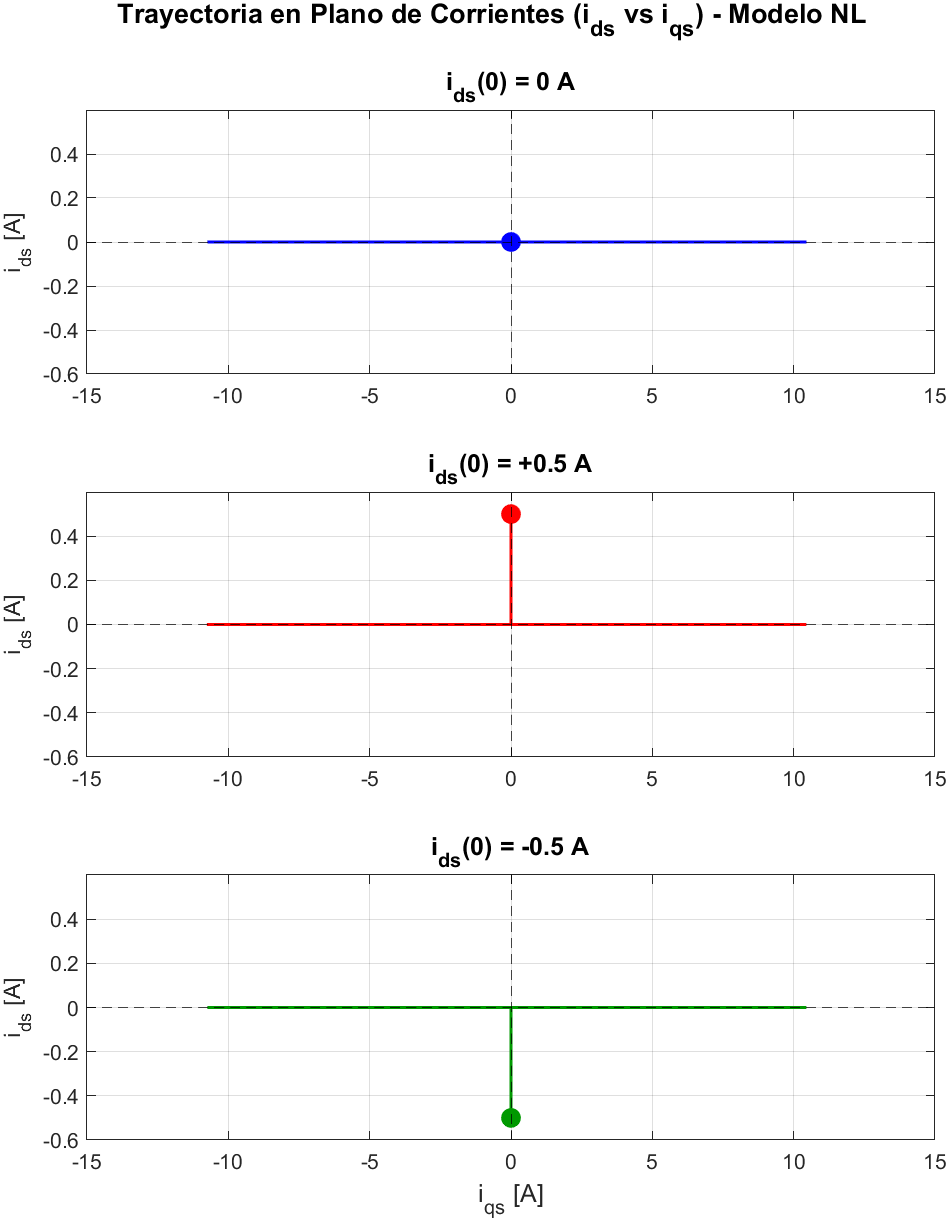
\includegraphics[width=0.9\textwidth]{imagenes/sim_ids_vs_iqs.png}
    \caption{Evolución de $i_{ds}^r(t)$ frente a $i_{qs}^r(t)$ para las tres condiciones iniciales $i_{ds}^r(0) \in \{0,\; +0{,}5,\; -0{,}5\}$~A (modelo NL). Independientemente del valor inicial, la corriente de eje $d$ converge al eje $i_{ds}^r = 0$ mientras $i_{qs}^r$ desarrolla el torque, evidenciando el desacople efectivo entre ambos ejes.}
    \label{fig:sim_ids_vs_iqs}
\end{figure}

\textbf{Análisis:}
\begin{itemize}
    \item En el \textbf{modelo LTI}, $i_{ds}^r(t)$ decae como exponencial pura:
    \begin{equation}
        i_{ds}^r(t) = i_{ds}^r(0) \cdot e^{-t/\tau_d}, \quad \tau_d = \frac{L_d}{R_{s0}} = \frac{6{,}6 \times 10^{-3}}{1{,}058} = 6{,}24 \text{ ms}
    \end{equation}
    completamente \textbf{desacoplado} del resto de los estados. Esto es consecuencia de la estructura diagonal por bloques de la matriz $A_{aug}$: el polo $p_d = -R_{s0}/L_d \approx -160{,}3$~rad/s es real, estable y no comparte autovector con ningún otro estado.

    \item En el \textbf{modelo NL}, $i_{ds}^r(t)$ también decae exponencialmente con la misma constante de tiempo. Aunque existe un acoplamiento residual NL del tipo $\omega_r \cdot L_q \cdot i_{qs}^r$, la ley de control mínima ($v_{ds}^r = -L_q i_{qs}^r \omega_r$) lo cancela exactamente, y la ley complementaria ($v_{qs} = v_{qs}^{r*} + \omega_r L_d i_{ds}^r$) elimina el efecto cruzado inverso.

    \item En ambos modelos, el efecto de $i_{ds}^r(0) \neq 0$ se extingue en $\approx 5\tau_d \approx 31$~ms, sin impacto apreciable sobre la dinámica mecánica ($\omega_m$, $\theta_m$) ni sobre $i_{qs}^r$. Esto justifica la hipótesis adoptada en la sección de linealización: la condición $i_{ds}^r(0) = 0$ no es restrictiva en la práctica, ya que cualquier valor inicial decae rápidamente a cero.
\end{itemize}

% =====================================================================
\subsubsection{Field Forcing y Field Weakening (Sub-ítem d)}
\label{sec:sim_item_d}

Se agrega una consigna de tensión en eje $d$, sumada a la ley de control mínima:
\begin{equation}
    v_{ds}^r(t) = \underbrace{-L_q \, i_{qs}^r(t) \, \omega_r(t)}_{\text{ley mínima}} + v_{ds}^{r*}(t), \quad
    v_{ds}^{r*}(t) = \begin{cases}
    0 & t < 0{,}5 \text{ s} \\
    +1{,}9596 \text{ V} & t \geq 0{,}5 \text{ s} \quad \text{(field forcing)}\\
    -1{,}9596 \text{ V} & t \geq 0{,}5 \text{ s} \quad \text{(field weakening)}
    \end{cases}
\end{equation}

donde $V_{ds}^{r*} = V_{qs,nom}^{r}/10 = 1{,}9596$~V. Se simula con $i_{ds}^r(0) = 0$~A para aislar el efecto de la tensión inyectada.

\begin{figure}[H]
    \centering
    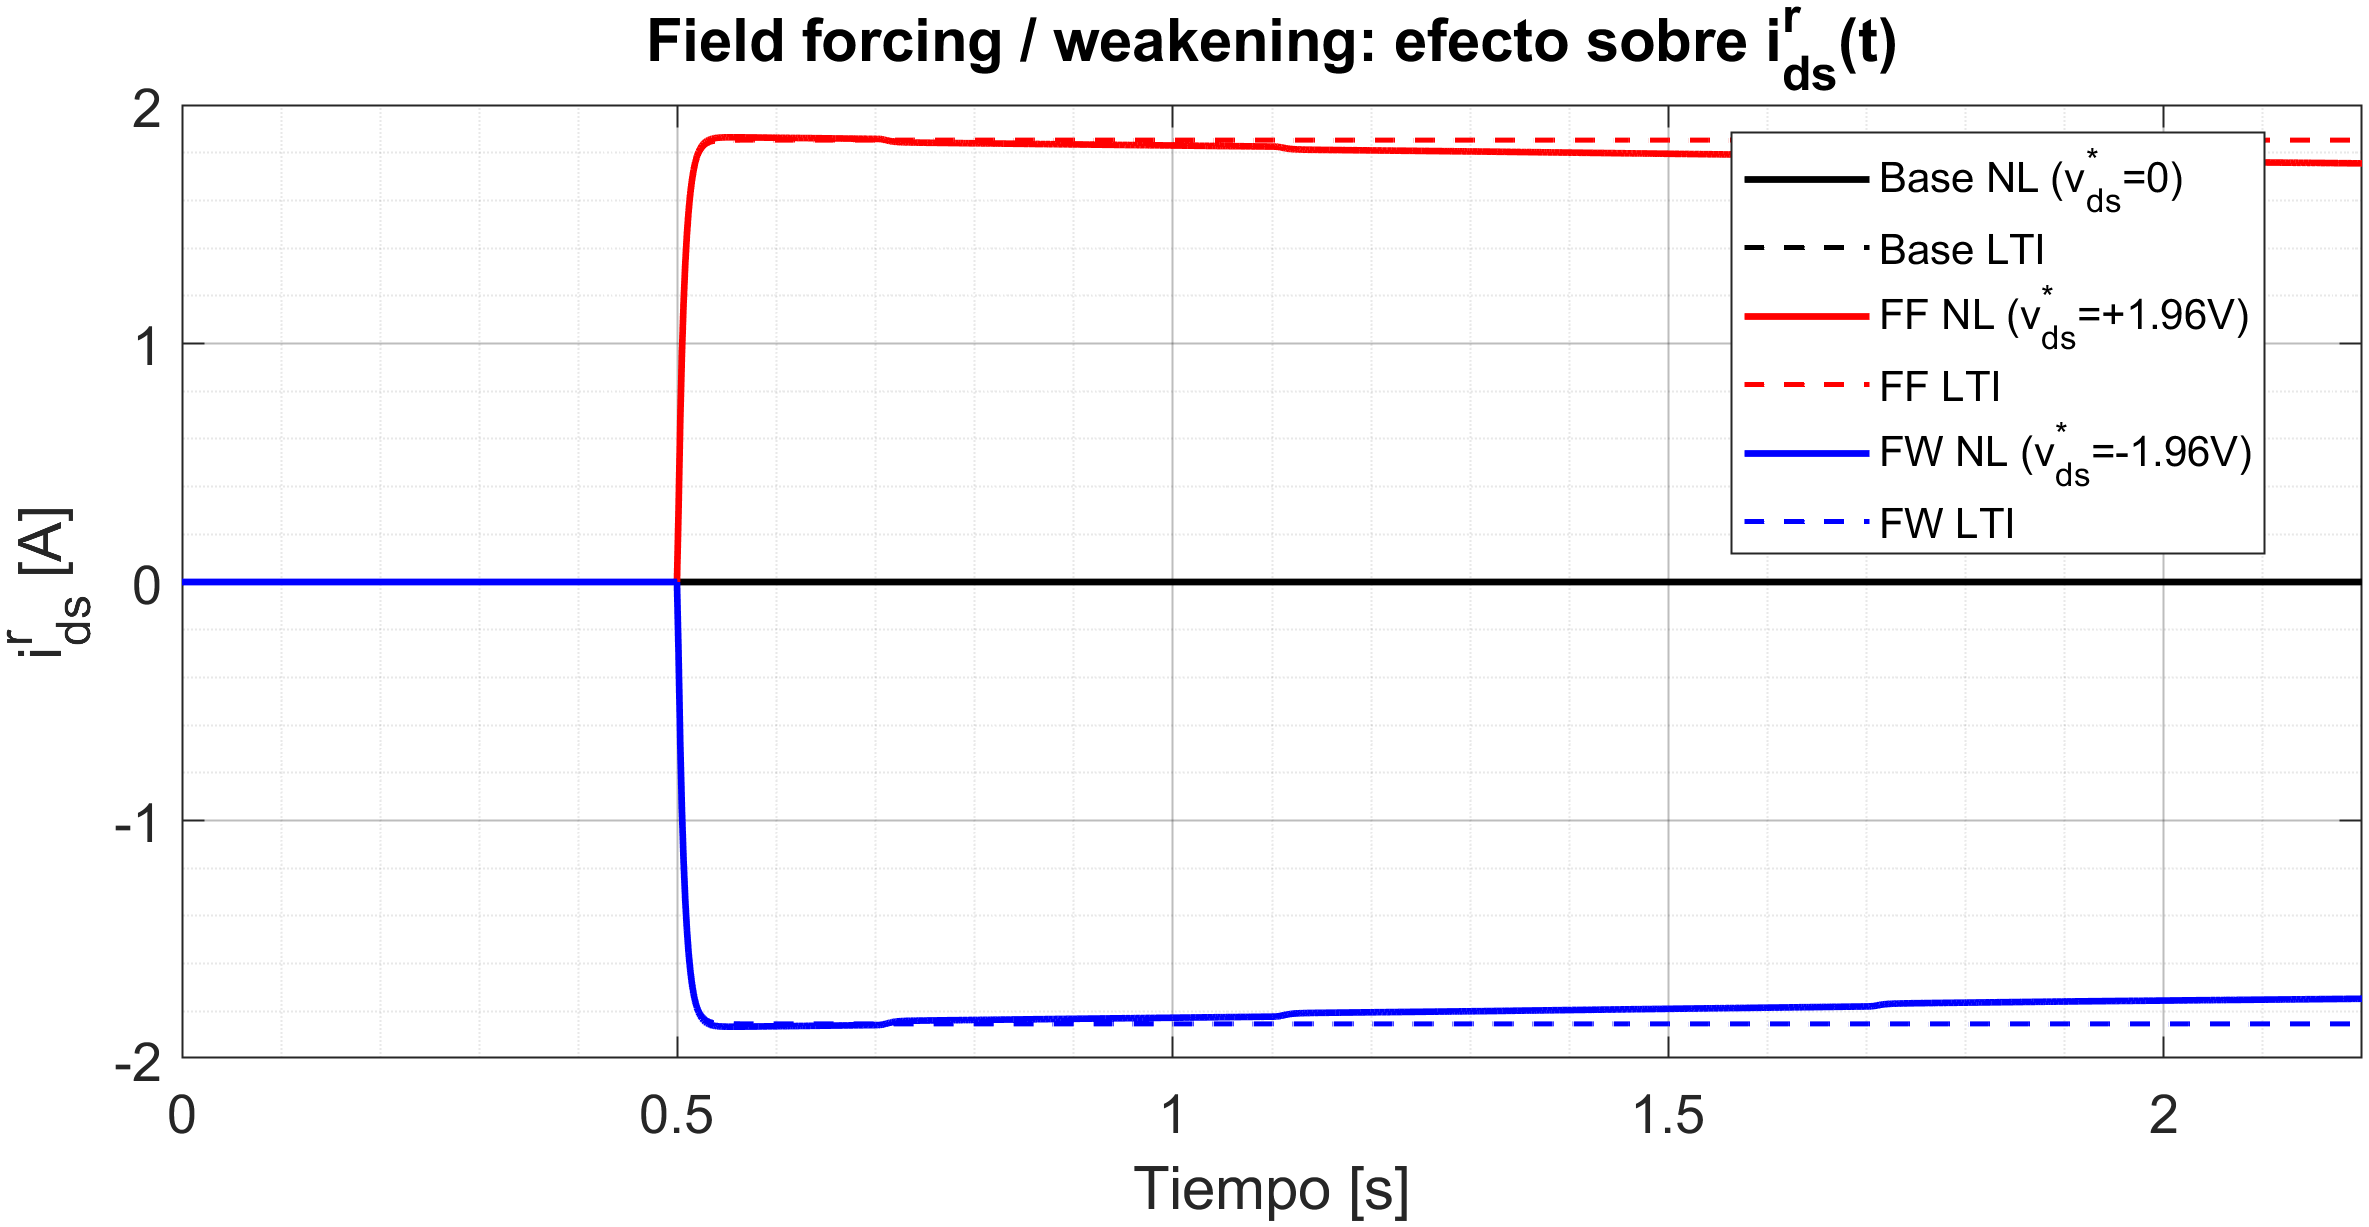
\includegraphics[width=\textwidth]{imagenes/sim_ff_ids.png}
    \caption{Efecto del field forcing ($v_{ds}^{r*} = +1{,}96$~V) y field weakening ($v_{ds}^{r*} = -1{,}96$~V) sobre $i_{ds}^r(t)$, comparado con el caso base ($v_{ds}^{r*} = 0$).}
    \label{fig:sim_field_forcing}
\end{figure}


\textbf{Análisis:}
\begin{itemize}
    \item En el \textbf{modelo LTI}, $v_{ds}^{r*}$ afecta \textbf{únicamente} a $i_{ds}^r$, que crece exponencialmente hasta su valor estacionario $i_{ds,ss}^r = v_{ds}^{r*}/R_{s0} = \pm 1{,}85$~A. Los demás estados ($\theta_m$, $\omega_m$, $i_{qs}^r$) permanecen \textbf{inalterados} por el desacoplamiento estructural de la matriz $A_{aug}$.

    \item En el \textbf{modelo NL}, $i_{ds}^r \neq 0$ introduce acoplamientos cruzados que el LTI no captura:
A partir del modelo no lineal, la dinámica de la corriente en el eje $d$ está gobernada por:
\begin{equation}
    \frac{di_{ds}^r(t)}{dt} = \frac{1}{L_d} \left[ v_{ds}^r(t) - R_s \cdot i_{ds}^r(t) + L_q \cdot i_{qs}^r(t) \cdot P_p \cdot \omega_m(t) \right]
\end{equation}

Por otro lado, el impacto directo sobre la fuerza generada se observa en la ecuación del torque electromagnético:
\begin{equation}
    T_m(t) = \frac{3}{2} P_p \left[ \lambda'^r_m + (L_d - L_q)i_{ds}^r(t) \right] i_{qs}^r(t)
\end{equation}

El signo de $i_{ds}^r$ define los mismos dos regímenes ya analizados físicamente en el estudio del modelo LPV: el \textbf{reforzamiento de campo} ($i_{ds}^r>0$) suma torque de reluctancia pero incrementa la fuerza contraelectromotriz ---reduciendo la velocidad máxima antes de saturar el inversor---, mientras que el \textbf{debilitamiento de campo} ($i_{ds}^r<0$) reduce el torque por amperio pero disminuye la fuerza contraelectromotriz, habilitando velocidades mayores dentro del límite de tensión. La simulación verifica ahora este comportamiento en forma dinámica.
\end{itemize}

%%%SECCION 516


\section{Diseño, Análisis y Simulación de Controlador de Movimiento en Cascada con Modulador de Torque}
\subsection{Diseño del Modulador de Torque}

En esta sección se desarrolla el diseño e implementación del modulador de torque equivalente, el cual operará como el controlador interno vectorial de corriente y torque del sistema. El objetivo principal de esta etapa es recibir una consigna de torque de referencia $(T_m^*)$ y generar las tensiones de comando necesarias en coordenadas rotóricas \(qd0\) del estator, logrando un lazo de control rápido y libre de acoplamientos indeseados. Para lograrlo, se implementa una estrategia de desacoplamiento completo que compensa activamente todas las retroalimentaciones físicas naturales de la planta, cancelando los acoplamientos magnéticos cruzados, las fuerzas contraelectromotrices y las caídas resistivas variables con la temperatura $(R_s(T_s^\circ))$.
\subsection{Desacoplamiento de retroalimentaciones naturales}
Recordando las ecuaciones \eqref{eq:vqs_rotor}, \eqref{eq:vds_rotor} y \eqref{eq:v0s_rotor}:
    \begin{equation*}
        v^r_{qs}(t)=R_s(T_s^\circ(t))i^r_{qs}(t) + L_q\frac{d i^r_{qs}(t)}{dt}+[\lambda'^r_m + L_d i^r_{ds}(t)]\omega_r(t)
    \end{equation*}
    \begin{equation*}
        v_{ds}^r(t)=R_s(T_s^\circ(t))i^r_{ds}(t)+L_d\frac{d i^r_{ds}(t)}{dt} - L_qi^r_{qs}(t)\omega_r(t)
    \end{equation*}
    \begin{equation*}
        v_{0s}(t)=R_s(T_s^\circ(t))i_{0s}(t)+L_{ls}\frac{d i_{0s}(t)}{dt}
    \end{equation*}
Se observan las retroalimentaciones naturales: la dependencia de la resistencia variable con la temperatura $T_s^\circ(t)$, el acoplamiento entre las corrientes $i_{qs}^r$ e $i_{ds}^r$, y las demás fuentes de no linealidad ya estudiadas anteriormente en el presente trabajo.

Por lo tanto, la propuesta principal es cancelar estos términos de retroalimentación física natural y obtener ecuaciones que relacionen la dinámica de las corrientes directamente con el voltaje, para implementar luego el modulador de torque de forma sencilla.

Esto lleva a proponer las siguientes ecuaciones, que al reemplazarse luego en \eqref{eq:vqs_rotor}, \eqref{eq:vds_rotor} y \eqref{eq:v0s_rotor} permiten obtener ecuaciones diferenciales en una forma útil.
\begin{equation}
v_{qs}^{r}(t) = v_{qs}^{r*}(t) 
+ R_s\!\big(T_s^{\circ}(t)\big)\, i_{qs}^{r}(t) 
+ \left[\lambda'^r_m + L_d\, i_{ds}^{r*}(t)\right] P_p\, \omega_m(t)
\label{eq:vqs_r}
\end{equation}

\begin{equation}
v_{ds}^{r}(t) = v_{ds}^{r*}(t) 
+ R_s\!\big(T_s^{\circ}(t)\big)\, i_{ds}^{r}(t) 
- L_q\, i_{qs}^{r*}(t)\, P_p\, \omega_m(t)
\label{eq:vds_r}
\end{equation}

\begin{equation}
v_{0s}(t) = v_{0s}^{*}(t) 
+ R_s\!\big(T_s^{\circ}(t)\big)\, i_{0s}(t)
\label{eq:v0s}
\end{equation}
Reemplazando, se obtiene:
\begin{equation}
    v_{qs}^{r*}(t) = L_q \frac{di_{qs}^r(t)}{dt}
    \label{eq:vqs_ref}
\end{equation}
\begin{equation}
    v_{ds}^{r*}(t) = L_d \frac{di_{ds}^r(t)}{dt}
    \label{eq:vds_ref}
\end{equation}
\begin{equation}
    v_{0s}^{*}(t) = L_{ls} \frac{di_{0s}(t)}{dt}
    \label{eq:v0s_ref}
\end{equation}
\begin{figure}[H]
    \centering
    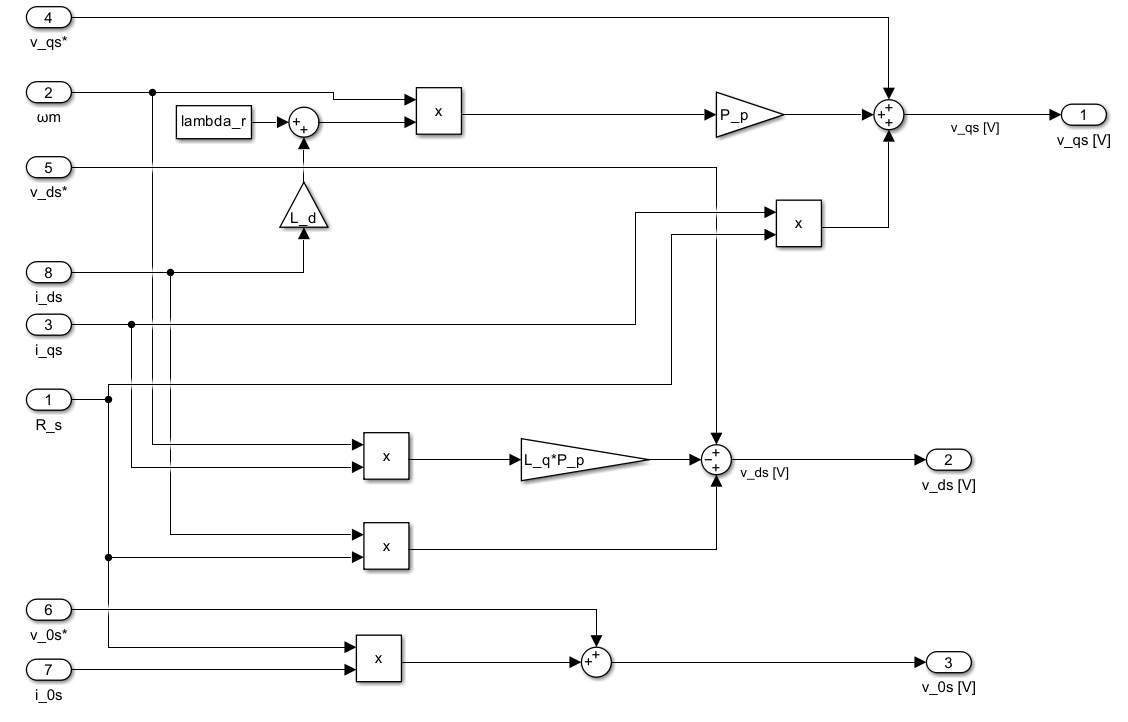
\includegraphics[width=0.8\textwidth]{imagenes/desacop_realimentacion_fisicas_naturales.png}
    \caption{Implementación en Simulink del desacoplamiento de las retroalimentaciones físicas naturales: las tensiones de referencia $v_{qd0s}^{r*}$ cancelan las caídas resistivas $R_s(T_s^\circ)\,i$, la fuerza contraelectromotriz y los acoplamientos cruzados entre los ejes $q$ y $d$.}
\end{figure}
\begin{figure}[H]
    \centering
    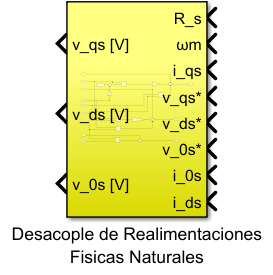
\includegraphics[width=0.4\textwidth]{imagenes/desacop_realimentacion_fisicas_naturales_bloque.png}
    \caption{Bloque (subsistema) equivalente del desacoplamiento de retroalimentaciones físicas naturales.}
\end{figure}
\subsubsection{Comparación: desacoplamiento de retroalimentaciones físicas naturales vs. linealización por retroalimentación NL}

Al contrastar la estrategia de linealización mediante el modulador de torque (que compensa las retroalimentaciones físicas naturales del sistema) con la linealización por retroalimentación NL mínima desarrollada en la etapa inicial a lazo abierto, aparecen diferencias relevantes en alcance matemático, flexibilidad operativa y manejo de la dinámica interna:

\begin{itemize}
    \item \textbf{Generalización del espacio de operación (liberación de $i_{ds}^r$):} 
    La estrategia de linealización previa imponía de forma estricta la condición $i_{ds}^r(t)=0$ para lograr el desacoplamiento entre el canal de flujo magnético y el de torque. En cambio, el desacoplamiento completo implementado en el modulador de torque generaliza el modelo y permite que la corriente del eje directo tome valores distintos de cero. Esto es clave porque habilita, de manera física, operaciones de debilitamiento o reforzamiento de campo según los requerimientos del accionamiento.
    
    \item \textbf{Grado de cancelación de las dinámicas naturales:} 
    La linealización por retroalimentación NL original se limitaba a cancelar los acoplamientos cruzados inductivos entre los ejes $q$ y $d$. El nuevo enfoque de desacoplamiento es más exhaustivo: inyecta tensiones de referencia calculadas para cancelar todas las retroalimentaciones naturales de la planta. Esto incluye no solo los acoplamientos cruzados, sino también la fuerza contraelectromotriz de los imanes permanentes y las caídas de tensión resistivas de los devanados.
    
    \item \textbf{Control explícito de la dinámica de corriente (asignación de polos):} 
    En la linealización inicial, la cancelación se realizaba sin ubicar explícitamente los polos del lazo interno de corriente, lo que limitaba el ajuste de la rapidez de respuesta. Con el desacoplamiento completo actual, las corrientes del estator pasan a responder de manera casi independiente, comportándose aproximadamente como integradores puros ante las entradas de tensión. Esto permite introducir un modulador de corriente estrictamente proporcional que ubica los polos del lazo interno en posiciones específicas (por ejemplo, $p_i=-5000$ rad/s), otorgando mayor control sobre la velocidad de respuesta en transitorios.
\end{itemize}


\subsubsection{Efecto de estimar la dependencia $R_s(T_s^\circ(t))$ vs. utilizar un valor nominal constante}

Al diseñar el modulador de torque equivalente encargado del desacoplamiento, surge la disyuntiva de cómo tratar la resistencia del estator. En la planta física, la resistencia $R_s$ depende de forma inevitable de la temperatura $T_s^\circ(t)$ debido al calentamiento progresivo por efecto Joule. El tratamiento de este parámetro define la robustez del controlador:

\begin{itemize}
    \item \textbf{Estimación en línea (resistencia variable):} 
    Si el controlador interno considera esta dependencia térmica y actualiza en tiempo real el valor de $R_s(T_s^\circ(t))$ a partir de las mediciones del sensor de temperatura, el cálculo de las tensiones de desacoplamiento resulta matemáticamente más preciso. Esto deriva en un comportamiento más robusto frente a cambios térmicos, al reducir perturbaciones cruzadas y errores de seguimiento durante transitorios y en régimen permanente.
    
    \item \textbf{Uso de valor nominal (resistencia constante):} 
    Si el controlador asume un valor nominal constante (típicamente el medido a temperatura ambiente), la compensación interna pierde exactitud a medida que la temperatura del devanado aumenta y se aleja del punto de referencia. En consecuencia, la tensión calculada para compensar la caída resistiva resulta insuficiente frente a la caída de tensión real en una máquina caliente.
\end{itemize}

Concretamente, en las simulaciones de esta sección el caso ``$R_s$ constante'' emplea $R_s(25\,^\circ\text{C}) \approx 1{,}04\ \Omega$ (la resistencia evaluada a la temperatura ambiente de operación), mientras que el caso ``$R_s$ variable'' actualiza $R_s(T_s^\circ(t)) = R_{sREF}\,[1+\alpha_{Cu}(T_s^\circ(t)-T_{sREF}^\circ)]$ con la medición del sensor de temperatura. La planta NL conserva su $R_s(T_s^\circ(t))$ real en ambos casos, por lo que la diferencia entre las curvas refleja únicamente el error de compensación del controlador.
%insertar aqui graficas
\begin{figure}[H]
    \centering
    
\includegraphics[width=0.6\textwidth]{imagenes/comp_torque_rs.png}
    \caption{Evolución temporal del torque neto ($T_{\text{neto}}$) en [N.m]. Se contrasta el comportamiento con resistencia estatórica constante (RS Cte., línea roja) y con resistencia estatórica variable (RS Variable, línea azul).}
    \label{fig:comparacion_torque_neto_RS}
\end{figure}

\begin{figure}[H]
    \centering
    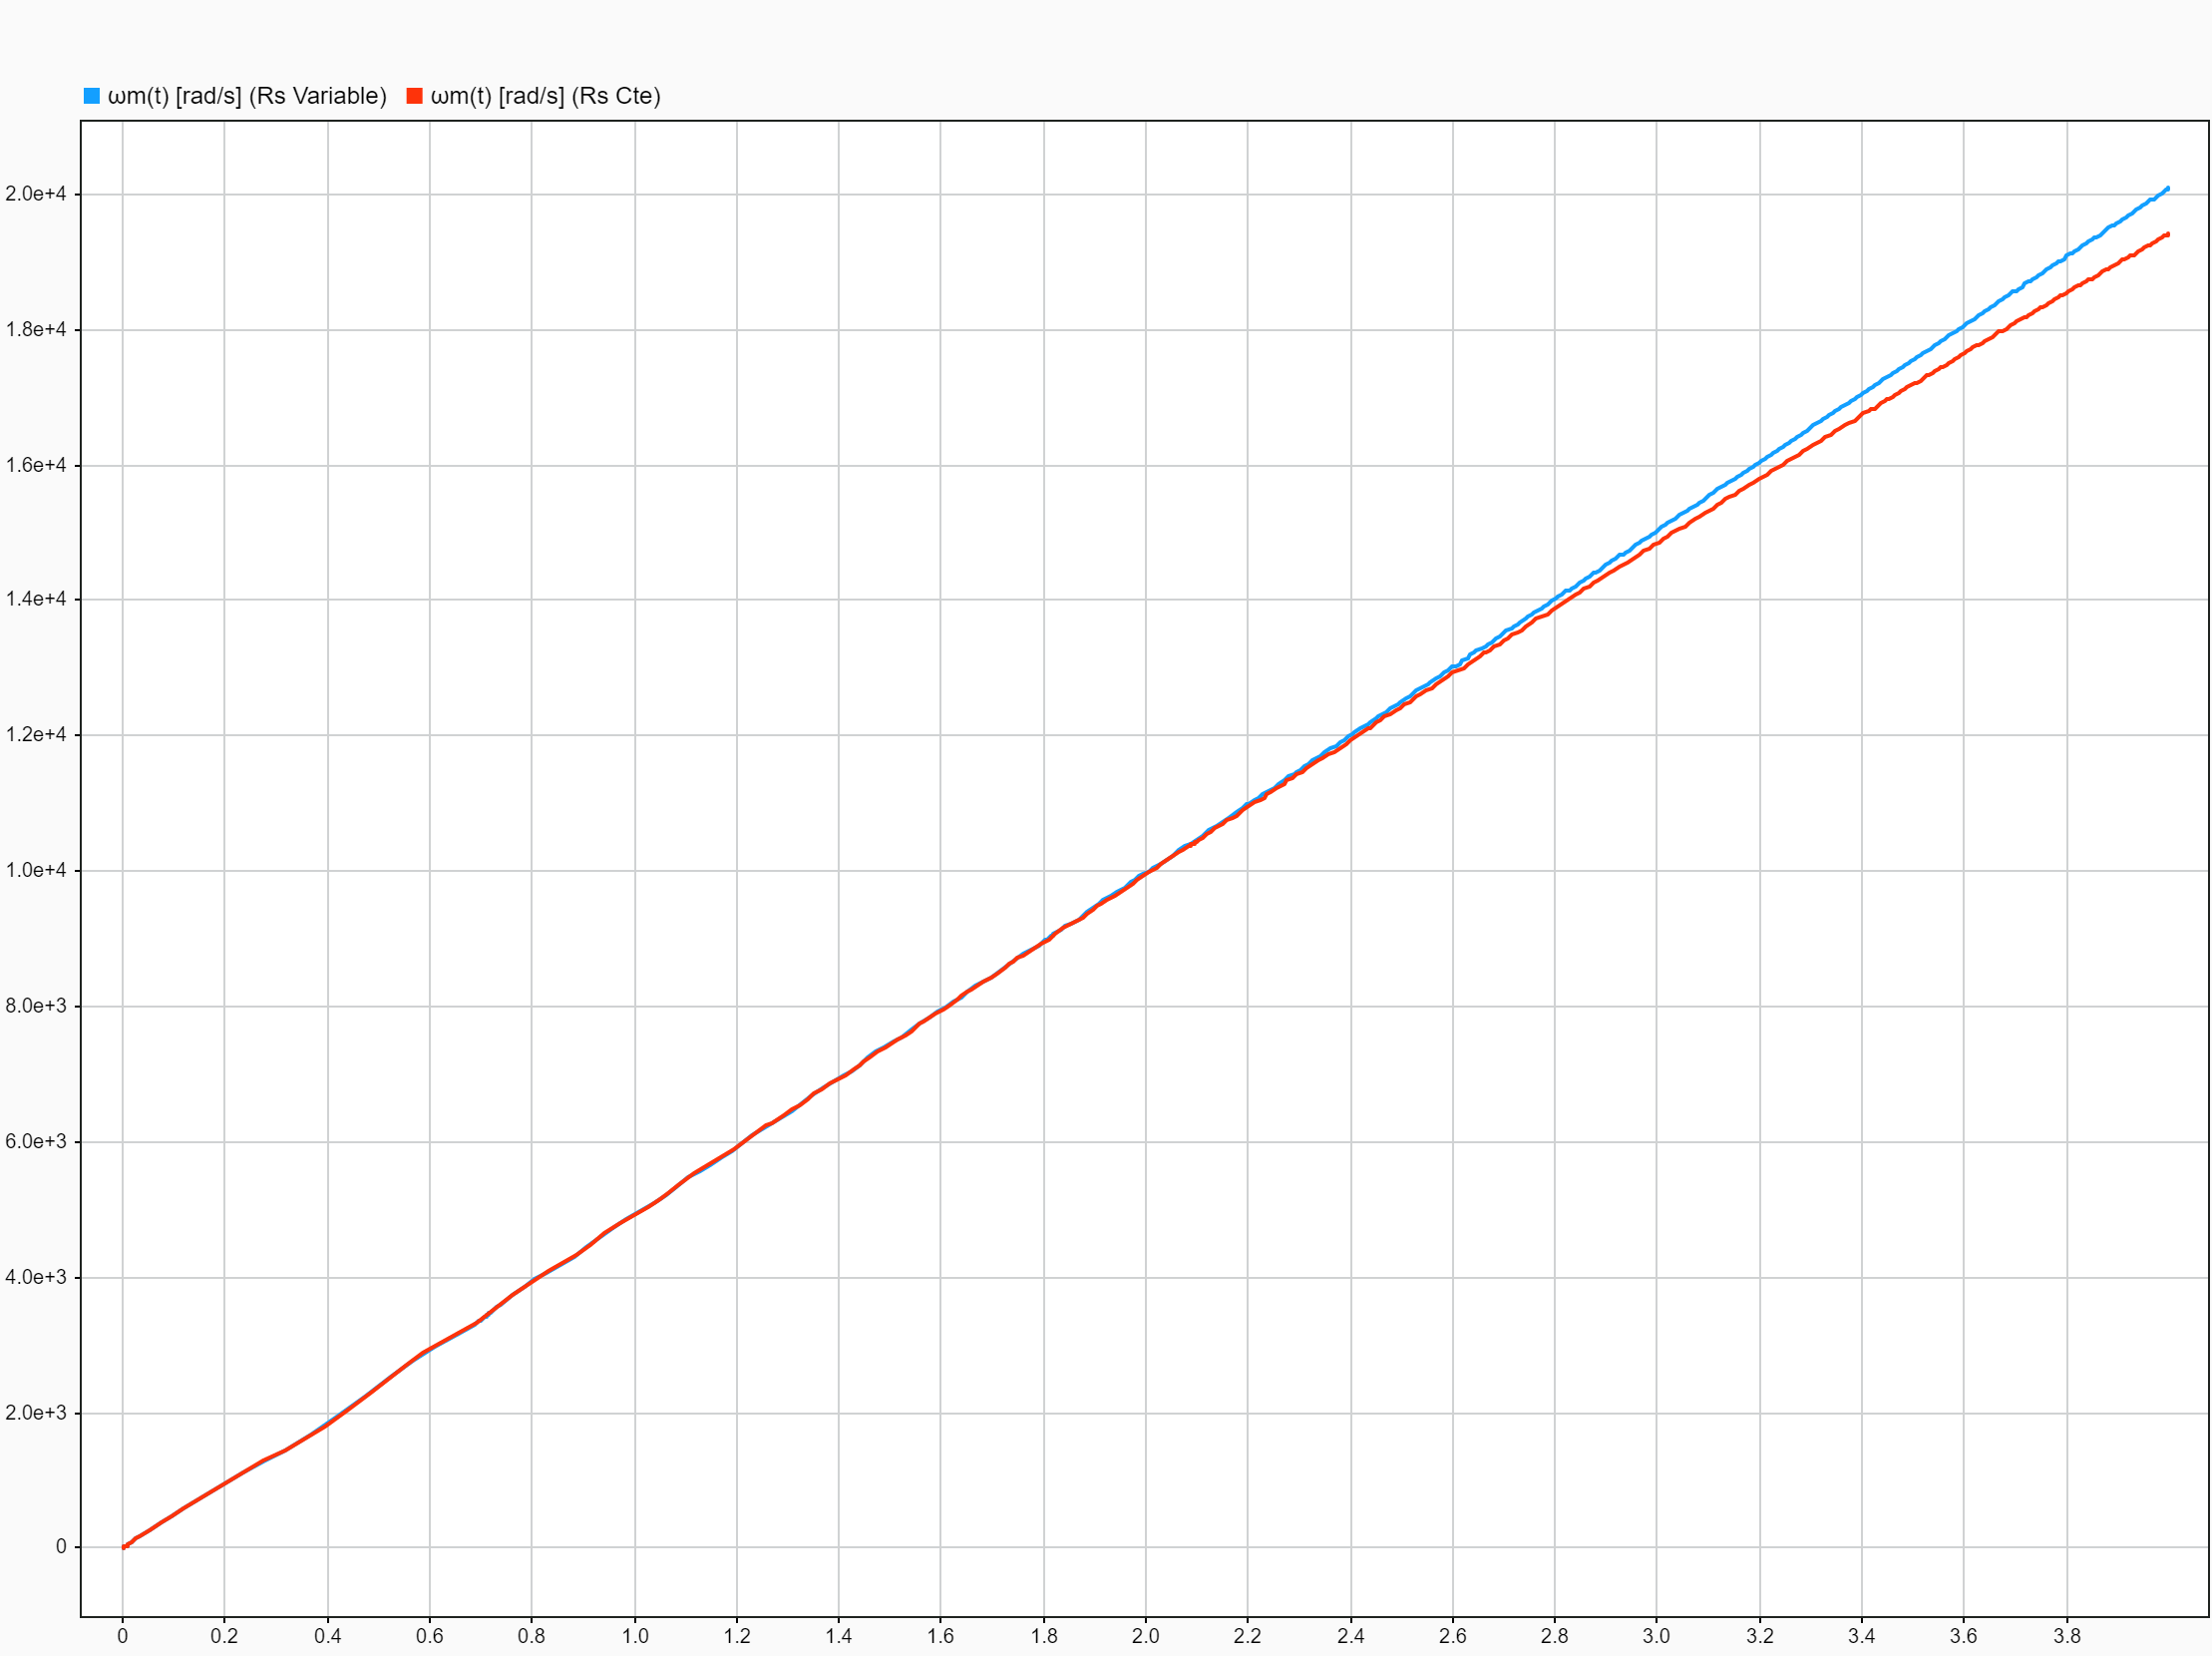
\includegraphics[width=0.6\textwidth]{imagenes/comp_velocidad_rs.png}
    \caption{Comportamiento de la velocidad angular mecánica ($\omega_m(t)$) en [rad/s] en función del tiempo. Se comparan las respuestas con resistencia estatórica constante (RS Cte., línea roja) y con resistencia estatórica variable (RS Variable, línea azul).}
    \label{fig:comparacion_velocidad_angular_RS}
\end{figure}
El impacto de no compensar la variación térmica se manifiesta en una degradación del desempeño global del sistema. Esta inexactitud en la cancelación resistiva produce un error en estado estacionario en las corrientes internas y, consecuentemente, en el torque electromagnético generado.

Como puede verse en la Fig. \ref{fig:comparacion_torque_neto_RS} y \ref{fig:comparacion_velocidad_angular_RS}, este déficit sostenido de torque aplicado tiene una repercusión directa y acumulativa sobre el comportamiento mecánico. Al entregar un torque ligeramente inferior al demandado por la consigna, se genera una divergencia progresiva en las curvas de velocidad angular. La trayectoria de velocidad del sistema que opera con un controlador de resistencia constante se desvía de forma creciente respecto de la trayectoria ideal, lo que evidencia la necesidad de un modelado térmico preciso para garantizar el desempeño exigido en regímenes de operación prolongados.

Cuantitativamente, al cabo de $4$~s con $R_s$ constante el torque neto entregado presenta un déficit cercano al $15\%$ respecto del caso con $R_s$ variable; dicho déficit, al integrarse en la dinámica mecánica, se traduce en un error en la posición del rotor $\theta_m$ de aproximadamente $4\%$. Esto confirma que estimar $R_s(T_s^\circ(t))$ en el controlador mejora apreciablemente la exactitud del desacoplamiento en regímenes prolongados, mientras que el uso de un valor constante resulta aceptable solo para intervalos cortos o cuando la deriva térmica es pequeña.
\subsection{Diseño de los Lazos de Control de Corrientes $\bm{i}_{qd0s}^r$}
Dado que la planta es de tipo 1, es posible aplicar una ley de control proporcional simple para lograr un error de estado estacionario nulo, por lo que se puede plantear:
\begin{equation}
    \bm{v}_{qd0s}^{r*}(t) = \bm{K_p} \big(\bm{i}_{qd0s}^{r*}(t)-\bm{i}_{qd0s}^{r}(t)\big)
\end{equation}
En forma escalar:
\begin{equation*}
\begin{aligned}
v_{qs}^{r*}(t) &= K_{pq} \left(i_{qs}^{r*}(t) - i_{qs}^{r}(t)\right) \\
v_{ds}^{r*}(t) &= K_{pd} \left(i_{ds}^{r*}(t) - i_{ds}^{r}(t)\right) \\
v_{0s}^{*}(t) &= K_{p0} \left(i_{0s}^{*}(t) - i_{0s}(t)\right)
\end{aligned}
\end{equation*}
Esto permite determinar la siguiente función de transferencia, reemplazando las ecuaciones \eqref{eq:vqs_ref}, \eqref{eq:vds_ref} y \eqref{eq:v0s_ref} en la ley de control:
\begin{gather*}
    L_qsI_{qs}^r(s) = K_{pq}\big(I_{qs}^{r*}(s)-I_{qs}^{r}(s)\big) \\ 
    \Big(L_qs+K_{pq}\Big)I_{qs}^r(s)=K_{pq}I_{qs}^{r*}(s) \\
    \frac{I_{qs}^r(s)}{I_{qs}^{r*}(s)} = \frac{1}{1+\frac{L_q}{K_{pq}}s}
\end{gather*}
Ídem para los demás ejes.
Queremos los polos en $p_i=-5000$~rad/s; por lo tanto, las ganancias quedan:
\[
K_{pq}=5000L_q=29~\Omega, \qquad
K_{pd}=5000L_d=33~\Omega, \qquad
K_{p0}=5000L_{ls}=4~\Omega.
\]

\textbf{Cambio de dinámica respecto del modelo LTI aumentado.} Esta respuesta de primer orden contrasta con la obtenida allí: la ley de control mínima más la complementaria cancelaban los acoplamientos cruzados pero \textit{dejaban} en la ecuación del eje $q$ la fuerza contraelectromotriz $\lambda'^r_m\,\omega_r$, por lo que $i_{qs}^r$ quedaba acoplada con $\omega_m$ formando un par de polos complejos $\lambda_{2,3} = -91{,}7 \pm j\,148$ ($\zeta = 0{,}527$, $\omega_n = 174$~rad/s, $\tau \approx 11$~ms): una dinámica oscilatoria subamortiguada e impuesta por la física, no designable. Aquí, en cambio, el desacople completo cancela también la fuerza contraelectromotriz, cada eje se reduce a un integrador puro y la asignación del polo en $-5000$~rad/s entrega una respuesta de primer orden con $\tau \approx 0{,}2$~ms: \textbf{sin oscilación, designable y más de un orden de magnitud más rápida} que la del LTI aumentado. Es justamente esta separación de escalas la que habilitará diseñar el lazo externo de movimiento mediante el método de sintonía serie.

\textbf{Sobre el agregado o no de acción integral.} La consigna pide investigar explícitamente si conviene sumar una acción integral a los lazos de corriente. La respuesta es \textbf{no}, y la razón es el principio del modelo interno: la planta de cada eje ya es de tipo 1 ($L\,di/dt = v^*$ contiene un integrador propio), por lo que el control proporcional alcanza error estacionario nulo ante una referencia escalón sin necesidad de un integrador adicional. Agregar un integrador convertiría el lazo abierto en tipo 2, lo que no mejora el seguimiento de escalones (ya era cero) y solo introduce desventajas: aumenta el orden del sistema, induce sobrepico, vuelve la sintonía más sensible al ruido de medición y trae riesgo de \textit{integrator windup} cuando el inversor satura. Por estas razones se conserva una ley puramente proporcional.
\begin{figure}[H]
    \centering
    
\includegraphics[width=0.6\textwidth]{imagenes/mod_corriente.png}
    \caption{Lazos de control de corriente $i_{qd0s}^{r}$ con acción proporcional, ubicando los polos del lazo interno en $p_i=-5000$~rad/s.}
\end{figure}
\begin{figure}[H]
    \centering
    
\includegraphics[width=0.2\textwidth]{imagenes/mod_corriente_subsystem.png}
    \caption{Subsistema del modulador (lazo proporcional) de corrientes.}
\end{figure}
\subsection{Incorporación de Consigna de Torque: Modulador de Torque}
Para el sistema electromagnético, la única forma de variar el torque es a través de la corriente. Por lo tanto, para incorporar esta nueva variable manipulada, es necesario diseñar un modulador de torque simple que traduzca la consigna a una consigna de corriente $i_{qs}^{r*}$. Se propone entonces aplicar una consigna de \textit{torque mecánico}, para que, al momento de aplicar la consigna, no sea necesario tener en cuenta la fricción ni la gravedad; para ello se implementa un \textit{precomputed torque} (torque precalculado).
\begin{equation}
    T_m^{\ast}(t) = T_m^{\ast\prime}(t) + b_{eq}\omega_m(t) + \frac{g\cdot k_l}{r}\sin{\Bigg( \frac{\theta_m(t)}{r}\Bigg)}
\end{equation}
Como se dijo, la idea principal es obtener una consigna de corriente, donde, aplicando control vectorial, se conseguirá una consigna de corriente en cuadratura $i_{qs}^{r*}$. Despejando de la ecuación \eqref{eq:torque_electromagnetico}:
    \begin{equation*}
            T_m^*(t) = \frac{3}{2} P_p \cdot \lambda'^r_m \cdot i^{r*}_{qs}(t) + \frac{3}{2} P_p (L_d-L_q)\cdot i^r_{ds}(t)\cdot i^{r*}_{qs}(t)
    \end{equation*}
\begin{gather*}
i_{qs}^{r*}(t)=
\frac{T_m^*(t)}
{\frac{3}{2}P_p\left[\lambda'^r_m+(L_d-L_q)i_{ds}^{r}(t)\right]} \\
i_{qs}^{r*}(t)= \frac{T_m^{\ast\prime}(t) + b_{eq}\omega_m(t) + \frac{g\cdot k_l}{r}\sin{\Big( \frac{\theta_m(t)}{r}\Big)}}{\frac{3}{2}P_p\left[\lambda'^r_m+(L_d-L_q)i_{ds}^{r}(t)\right]}
\end{gather*}
Puede observarse en la ecuación anterior que la variable $i_{ds}^r$ quedaría como un parámetro más, lo que habilita la posibilidad de dos casos ya vistos anteriormente en el presente trabajo.
\begin{itemize}
    \item $i_{ds}^r = 0$: si se aplica esta consigna, el torque depende únicamente de la corriente en eje $q$ y del flujo de los imanes permanentes, lo que resulta suficiente para la mayoría de los casos.
    \item $i_{ds}^r \neq 0$: ya sea por reforzamiento o debilitamiento de campo, $i_{ds}^r$ actuaría como una consigna adicional para situaciones en las que el rango de voltaje del inversor no sea suficientemente amplio.
\end{itemize}
\begin{figure}[H]
    \centering
    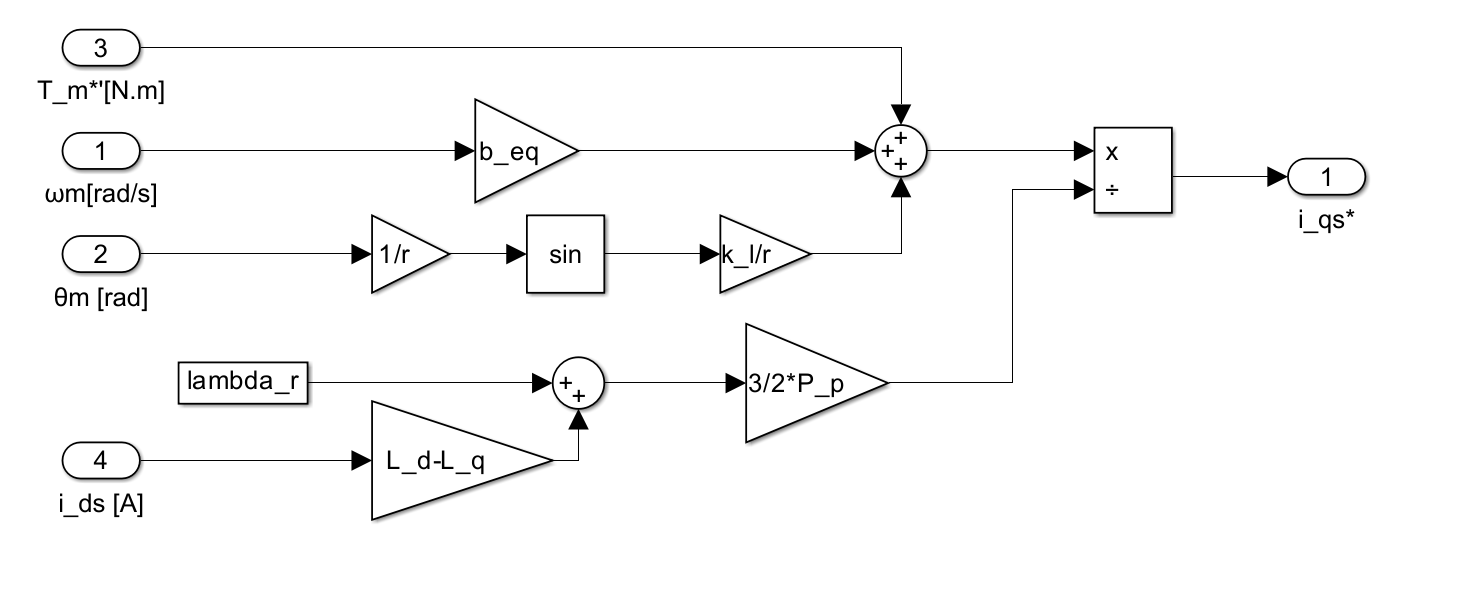
\includegraphics[width=0.75\linewidth]{imagenes/mod_torque_diagram.png}
    \caption{Diagrama de bloques del modulador de torque implementado.}
\end{figure}
\subsection{Controlador externo de posición y velocidad}

Dado que el objetivo del presente trabajo es controlar la posición y la velocidad del eje, se propone la implementación de un controlador PID que manipule directamente el torque, aplicando consignas sobre el \textit{Modulador de Torque}. La entrada de referencia del lazo es el \textit{setpoint} de posición articular definido por la guía, $q_1^*(t) \equiv \frac{1}{r}\,\theta_m^*(t)$, incorporado al diagrama de bloques del sistema. Para ello, se propone la siguiente ley de control:
\begin{equation}
    T_m^{*\prime}(s)= b_a\,E_\omega(s) + K_{sa}\,E_{\theta_m}(s)+K_{sia}\,\frac{E_{\theta_m}(s)}{s}
    \label{eq:ley_pid_522}
\end{equation}

Las ganancias del controlador se sintonizan por el método de \textbf{sintonía serie}, para un amortiguamiento $\zeta = 0{,}75$ y una frecuencia natural $\omega_n = 800\ \frac{rad}{s}$: se obtiene el polinomio característico del lazo cerrado en función de las ganancias (polinomio \emph{estructural}), se construye el polinomio \emph{requerido} a partir de los polos deseados y se igualan ambos, coeficiente a coeficiente.

\textbf{Dinámica de lazo cerrado.} El diseño se apoya en dos propiedades ya establecidas de la arquitectura en cascada:
\begin{itemize}
    \item Los lazos de corriente responden con polos en $p_i=-5000$~rad/s, más de seis veces más rápidos que la especificación del lazo externo ($\omega_n=800$~rad/s); a la escala temporal del lazo de movimiento puede considerarse, entonces, que el torque generado sigue instantáneamente a su consigna: $T_m(t) \approx T_m^{*}(t)$.
    \item El \textit{precomputed torque} del modulador compensa por prealimentación la fricción $b_{eq}\,\omega_m$ y el término gravitatorio, de modo que la planta mecánica vista por el controlador externo se reduce a un doble integrador sobre el que actúa la perturbación de carga no compensada:
\end{itemize}
\begin{equation}
    J_{eq}\,\ddot{\theta}_m(t) = T_m^{*\prime}(t) - \frac{T_{ld}(t)}{r}
    \label{eq:planta_externa_522}
\end{equation}

Transformando por Laplace y cerrando el lazo con la ley \eqref{eq:ley_pid_522} --- donde el generador de trayectoria garantiza $\omega_m^*(t)=\frac{d}{dt}\theta_m^*(t)$ y, por lo tanto, $E_\omega(s) = s\,E_{\theta_m}(s)$ ---:
\begin{gather*}
    J_{eq}s^2\,\Theta_m(s) = \Big(b_a s + K_{sa}+\frac{K_{sia}}{s}\Big)\big[\Theta_m^{\ast}(s)-\Theta_m(s)\big] - \frac{T_{ld}(s)}{r}\\
    \Theta_m(s)\Big(J_{eq}s^3+b_as^2 + K_{sa}s+K_{sia}\Big)=\Big(b_as^2 + K_{sa}s+K_{sia}\Big)\Theta_m^{\ast}(s) - \frac{s}{r}\,T_{ld}(s)
\end{gather*}
\begin{equation}
    \Theta_m(s)=\underbrace{\frac{b_as^2 + K_{sa}s+K_{sia}}{J_{eq}s^3+b_as^2 + K_{sa}s+K_{sia}}}_{G_{\theta^*}(s)}\,\Theta_m^{\ast}(s)\;-\;\underbrace{\frac{s/r}{J_{eq}s^3+b_as^2 + K_{sa}s+K_{sia}}}_{G_{T_{ld}}(s)}\,T_{ld}(s)
    \label{eq:tf_lazo_522}
\end{equation}

Ambas funciones de transferencia comparten el mismo denominador. El factor $s$ en el numerador de $G_{T_{ld}}(s)$ evidencia el efecto de la acción integral: una perturbación de carga constante se rechaza en forma exacta en régimen permanente ($G_{T_{ld}}(0)=0$). El \textbf{polinomio estructural} del lazo cerrado, en forma mónica, resulta:
\begin{equation}
    \boxed{\;P_e(s) = s^3+\frac{b_a}{J_{eq}}\,s^2+\frac{K_{sa}}{J_{eq}}\,s+\frac{K_{sia}}{J_{eq}}\;}
    \label{eq:pe_522}
\end{equation}

\textbf{Polinomio requerido.} Los tres polos de lazo cerrado se asignan a partir de las especificaciones: un polo real en $-\omega_n$ y un par complejo conjugado de parámetros $\zeta$ y $\omega_n$. El polinomio requerido y su expansión resultan:
\begin{gather}
    P_r(s) = (s+\omega_n)\left(s^2 + 2\zeta\omega_n s + \omega_n^2\right)\notag\\
    \boxed{\;P_r(s) = s^3 + \omega_n(2\zeta+1)\,s^2 + \omega_n^2(2\zeta+1)\,s + \omega_n^3\;}
    \label{eq:pr_522}
\end{gather}

La Fig.~\ref{fig:polos_pr_522} ilustra la configuración asignada: el polo real en $-\omega_n$ y el par complejo conjugado $-\zeta\omega_n \pm j\,\omega_n\sqrt{1-\zeta^2}$. Una propiedad notable de esta elección es que \textbf{los tres polos comparten la misma frecuencia natural} $\omega_n$, es decir, yacen sobre la circunferencia de radio $\omega_n$ del semiplano izquierdo.

\begin{figure}[H]
    \centering
    \begin{tikzpicture}[scale=0.85,
        pole/.style={draw=black, fill=blue!75, rectangle, inner sep=2.5pt, minimum size=7pt}]
      % zeta = 0.75, omega_n = 800 rad/s ; escala del dibujo: 1 unidad = 200 rad/s
      \def\polwn{4}
      \def\polsig{3}        % zeta*omega_n = 600 rad/s
      \def\polwd{2.6458}    % omega_n*sqrt(1-zeta^2) = 529.2 rad/s
      % Semicirculo punteado de radio omega_n (semiplano izquierdo)
      \draw[dashed] (0,\polwn) arc[start angle=90, end angle=270, radius=\polwn];
      % Ejes
      \draw[-stealth] (-5,0) -- (1.5,0) node[below right] {$\sigma$};
      \draw[-stealth] (0,-4.8) -- (0,5);
      \node[left] at (-0.30,4.45) {$j\omega$};
      % Linea punteada vertical que une los polos conjugados
      \draw[dotted, thick] (-\polsig,\polwd) -- (-\polsig,-\polwd);
      % Flecha que indica el radio omega_n
      \draw[-stealth, thick] (0,0) -- (160:\polwn);
      \node at (150:2.4) {$\omega_n$};
      % Polo real en -omega_n
      \node[pole] at (-\polwn,0) {};
      \node[below left=1pt] at (-\polwn,-0.05) {$-\omega_n$};
      % Polos conjugados
      \node[pole] at (-\polsig,\polwd) {};
      \node[pole] at (-\polsig,-\polwd) {};
    \end{tikzpicture}
    \caption{Configuración de polos asignada por el polinomio requerido $P_r(s)$: polo real en $-\omega_n$ y par complejo conjugado de parámetros $\zeta$ y $\omega_n$. Los tres polos comparten la frecuencia natural $\omega_n$: yacen sobre la circunferencia punteada de radio $\omega_n$.}
    \label{fig:polos_pr_522}
\end{figure}

\textbf{Igualación de coeficientes y despeje de las ganancias.} Imponiendo $P_e(s) = P_r(s)$ coeficiente a coeficiente:
\begin{equation}
\begin{cases}
\dfrac{b_a}{J_{eq}} = \omega_n(2\zeta+1) \\[10pt]
\dfrac{K_{sa}}{J_{eq}} = \omega_n^2(2\zeta+1) \\[10pt]
\dfrac{K_{sia}}{J_{eq}} = \omega_n^3
\end{cases}
\label{eq:igualacion_522}
\end{equation}

Cada ganancia aparece en un único coeficiente --- consecuencia de que la cascada ya absorbió la dinámica eléctrica en el lazo interno ---, por lo que el despeje es directo:
\begin{equation}
    \boxed{\;b_a = J_{eq}\,\omega_n(2\zeta+1)\;}\qquad
    \boxed{\;K_{sa} = J_{eq}\,\omega_n^2(2\zeta+1)\;}\qquad
    \boxed{\;K_{sia} = J_{eq}\,\omega_n^3\;}
    \label{eq:ganancias_522}
\end{equation}

\textbf{Valores numéricos.} Evaluando \eqref{eq:ganancias_522} con $\zeta=0{,}75$, $\omega_n=800$~rad/s y la inercia equivalente nominal ($m_l=0$), las ganancias del controlador resultan:
\begin{equation*}
\begin{aligned}
    b_a &= J_{eq}\,\omega_n(2\zeta+1) = 0{,}0396\ \frac{N\cdot m}{rad/s} \\
    K_{sa} &= J_{eq}\,\omega_n^2(2\zeta+1) = 31{,}656\ \frac{N\cdot m}{rad} \\
    K_{sia} &= J_{eq}\,\omega_n^3 = 10129{,}778\ \frac{N\cdot m}{rad\cdot s}
\end{aligned}
\end{equation*}

\subsubsection{Ubicación de los polos en el plano $s$ y migración ante variación de carga}

La Fig.~\ref{fig:mapa_polos_522} ubica en el plano $s$ los polos de las tres dinámicas que conviven en la arquitectura en cascada, para el diseño nominal:
\begin{itemize}
    \item \textbf{Planta a lazo abierto} (modelo LTI aumentado): el integrador en $s=0$, el par de polos electromecánico en $-91{,}7 \pm j148$ y el polo residual de $i_{ds}^r$ en $-160{,}3$~rad/s.
    \item \textbf{Lazos de corriente} (proporcionales): $-5000$~rad/s en los tres ejes.
    \item \textbf{PID de movimiento} (lazo cerrado, diseño nominal): un polo real en $-800$~rad/s y un par complejo en $-600 \pm j529$~rad/s ($\zeta = 0{,}75$, $\omega_n = 800$~rad/s), raíces de $J_{eq}(s+\omega_n)(s^2+2\zeta\omega_n s + \omega_n^2)$.
\end{itemize}

Se verifica la \textbf{separación de escalas} que sustenta el diseño en cascada: los polos del lazo externo de movimiento ($\approx 800$~rad/s) son sensiblemente más lentos que los lazos de corriente ($5000$~rad/s) y, a la vez, más rápidos que la dinámica dominante de la planta original ($\omega_n \approx 174$~rad/s). Esto justifica diseñar cada lazo suponiendo que el lazo interior es prácticamente instantáneo.

\begin{figure}[H]
    \centering
    
\includegraphics[width=\textwidth]{imagenes/mapa_polos_5_2_2.png}
    \caption{Polos en el plano $s$ (cuadrados sólidos, diferenciados por color): planta a lazo abierto (azul), lazos de corriente (verde, $-5000$) y polos de lazo cerrado del PID de movimiento (rojo, $-800$ y $-600\pm j529$). Izquierda: vista completa (separación de escalas); derecha: zoom planta vs.\ PID.}
    \label{fig:mapa_polos_522}
\end{figure}

\textbf{Migración ante variación extrema de los parámetros de carga.} El controlador se sintoniza con la inercia nominal $J_{eq}$ ($m_l = 0$). Como la inercia equivalente \textbf{no} se reajusta en línea (las ganancias $b_a$, $K_{sa}$, $K_{sia}$ son fijas), un cambio en la masa de carga $m_l \in [0;\,1{,}5]$~kg modifica $J_{eq}$ y corre los polos de lazo cerrado, que pasan a ser las raíces de $J_{eq}\,s^3 + b_a s^2 + K_{sa} s + K_{sia}$. La variación de la fricción de carga $b_l$, en cambio, no afecta esta migración: el modulador de torque compensa $b_{eq}\,\omega_m$ por prealimentación, de modo que el efecto dominante de la carga sobre el lazo cerrado proviene de la inercia $J_{eq}$, que no se compensa. La Tabla~\ref{tab:migracion_pid} y la Fig.~\ref{fig:migracion_pid} resumen el resultado.

\begin{table}[H]
\centering
\caption{Migración de los polos de lazo cerrado del PID ante variación de $m_l$ (ganancias fijas nominales).}
\label{tab:migracion_pid}
\renewcommand{\arraystretch}{1.2}
\footnotesize
\begin{tabular}{|c|c|c|c|c|}
\hline
$m_l$ [kg] & $J_{eq}$ [kg$\cdot$m$^2$] & Par complejo [rad/s] & Polo real [rad/s] & $\zeta$ \\
\hline
\textbf{0,00} & $\mathbf{1{,}98\times10^{-5}}$ & $\mathbf{-600{,}0 \pm j\,529{,}2}$ & $\mathbf{-800{,}0}$ & $\mathbf{0{,}750}$ \\
0,50 & $2{,}85\times10^{-5}$ & $-421{,}7 \pm j\,687{,}9$ & $-546{,}6$ & $0{,}523$ \\
1,00 & $3{,}72\times10^{-5}$ & $-294{,}1 \pm j\,696{,}5$ & $-477{,}1$ & $0{,}389$ \\
\textbf{1,50} & $\mathbf{4{,}58\times10^{-5}}$ & $\mathbf{-212{,}6 \pm j\,677{,}7}$ & $\mathbf{-438{,}2}$ & $\mathbf{0{,}299}$ \\
\hline
\end{tabular}
\end{table}

\begin{figure}[H]
    \centering
    
\includegraphics[width=0.75\textwidth]{imagenes/migracion_polos_pid.png}
    \caption{Migración de los polos de lazo cerrado del PID al variar $m_l$ de $0$ a $1{,}5$~kg con ganancias fijas (cuadrados sólidos, colorbar en $m_l$). El nominal ($m_l=0$) se marca con rombo sólido y el peor caso ($m_l=1{,}5$) con cuadrado sólido.}
    \label{fig:migracion_pid}
\end{figure}

Del análisis se desprende que, al aumentar la carga, los polos de lazo cerrado se \textbf{acercan al eje imaginario} y el \textbf{amortiguamiento cae de $\zeta=0{,}75$ a $\zeta\approx0{,}30$}, mientras que la frecuencia natural se mantiene aproximadamente constante ($\omega_n \approx 710$--$825$~rad/s). Es decir, con ganancias fijas el sistema permanece estable en todo el rango de carga, pero la respuesta se vuelve \textbf{notablemente más oscilatoria} en el peor caso ($m_l=1{,}5$~kg). Esto justificaría, si se exigiera conservar el amortiguamiento especificado en todo el rango, un esquema de control robusto o el agendado de las ganancias con la inercia estimada.

\subsection{Incorporación y diseño de observador de estado de orden reducido para $\theta_m(t)$ y $\omega_m(t)$}
Se pretende estimar la velocidad del motor a partir del sensado de la posición, suponiendo por lo tanto, que no se dispone de un tacómetro. Esta estimación es posible debido al análisis que se realizó anteriormente (\textit{Controlabilidad y Observabilidad}) donde también se demuestra que no es observable la posición a partir de la velocidad.
\subsubsection{Modelo del subsistema mecánico}
Para implementar un observador de orden reducido no es necesario plantear todas las ecuaciones de estado, en este caso, el único subsistema involucrado en la estimación es el mecánico, que, si consideramos que ya se desacopló el término $-b_{eq}\omega_m(t)$ nos queda:
\begin{gather}
\begin{aligned}
    \dot\theta_m(t) &= \omega_m(t) \\
    \dot \omega_m(t) &= \frac{1}{J_{eq}}\Big(T'_m(t)-\frac{T_l(t)}{r}\Big)
\end{aligned}
\end{gather}
Que en forma matricial:
\begin{gather*}
    \bm{\dot x}(t)
=
\begin{bmatrix}
    0 & 1 \\ 0 & 0
\end{bmatrix}
\bm{x}(t)
+
\begin{bmatrix}
    0 \\ \frac{1}{J_{eq}} 
\end{bmatrix}
    u(t)
\\
y(t) =
\begin{bmatrix}
    1 & 0
\end{bmatrix}
\bm{x}(t)
\end{gather*}
Donde:
\begin{gather*}
\bm{\dot x}(t)=
\begin{bmatrix}
    \dot\theta_m(t) \\ \dot\omega_m(t)
\end{bmatrix},
\quad
\bm{x}(t)=
\begin{bmatrix}
    \theta_m(t) \\ \omega_m(t)
\end{bmatrix},
\quad
\bm{x}(0)=
\begin{bmatrix}
    \theta_m(0) \\ \omega_m(0)
\end{bmatrix}, \\[6pt]
u(t)=T_m'(t),
\quad
y(t)=\theta_m(t),
\quad
\bm{A}=\begin{bmatrix}
    0 & 1\\ 0 & 0
\end{bmatrix},
\quad
\bm{C}=\begin{bmatrix}
    1 & 0
\end{bmatrix}.
\end{gather*}
    
\subsubsection{Diseño del observador}
    El observador de estados reducido se basará en el observador de Luenberger, cuya dinámica sigue una ley de control proporcional al error entre la salida medida y la estimada.
    \begin{gather*}
    \begin{aligned}
    \dot{\bar{\bm{x}}}(t)&=
    \bm{A}\bar{\bm{x}}(t) +
    \begin{bmatrix}
    0 \\ \frac{1}{J_{eq}}
    \end{bmatrix}u(t)+
    \bm{K}_e\big(y(t)-\bm{C}\bar{\bm{x}}(t)\big)\\
    \dot{\bar{\bm{x}}}(t)&=
    \big(\bm{A}-\bm{K}_e\bm{C}\big)\bar{\bm{x}}(t) +
    \begin{bmatrix}
    0 \\ \frac{1}{J_{eq}}
    \end{bmatrix}u(t)+\bm{K}_e\,y(t)
    \end{aligned}
    \end{gather*}
    Definiendo el vector de ganancias del observador $\bm{K}_e$, cuyas componentes son las ganancias del estimador $K_{e\theta_m}$ y $K_{e\omega_m}$:
    \begin{equation*}
        \bm{K}_e=
        \begin{bmatrix}
            K_{e\theta_m}\\
            K_{e\omega_m}
        \end{bmatrix}
    \end{equation*}
    Lo que resulta en el siguiente polinomio característico:
    \begin{gather*}
    \begin{aligned}
        \det\!\left[s\bm{I}-\left(\bm{A}-\bm{K}_e\bm{C}\right)\right]&=0,\\
        \begin{bmatrix}
            s & 0 \\ 
            0 & s
        \end{bmatrix}-
        \begin{bmatrix}
            0 & 1 \\
            0 & 0
        \end{bmatrix}+
        \begin{bmatrix}
            K_{e\theta_m} & 0 \\
            K_{e\omega_m} & 0
        \end{bmatrix} &=0,
        \\
        s^2 + s K_{e\theta_m}+K_{e\omega_m}&=0
    \end{aligned}
    \end{gather*}
    Se propone en la consigna, sintonizar estas ganancias de tal manera de obtener ambos polos en $p_{obs\,1,2}=-3200 \frac{rad}{s}$, y siendo el polinomio deseado:
    \begin{gather*}
        p_{des} = (s-p_{obs\,1,2})^2=s^2-2p_{obs\,1,2}s+p_{obs\,1,2}^2
    \end{gather*}
    Comparando con el pol. característico:
    \begin{equation}
        s^2 + s K_{e\theta_m}+K_{e\omega_m}=s^2-2p_{obs\,1,2}s+p_{obs\,1,2}^2
    \end{equation}
    Resultando entonces en las siguientes ganancias:
    \begin{gather}
        K_{e\theta_m} = 6400\ \mathrm{s}^{-1}\\K_{e\omega_m}=3200^2=1{,}024\times10^7\ \mathrm{s}^{-2}
    \end{gather}
    \begin{figure}[H]
        \centering
        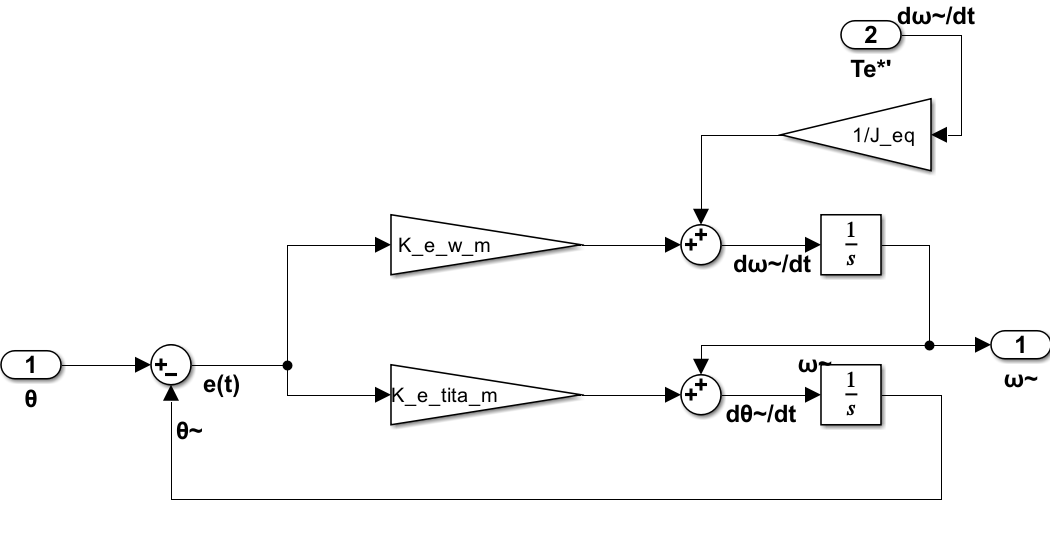
\includegraphics[width=0.8\linewidth]{imagenes/observador_diagram.png}
        \caption{Diagrama de bloques del observador de estados reducido}
    \end{figure}
    \subsection{Simulación en tiempo continuo con modelo completo NL}
    \subsubsection{Consigna trapezoidal de posición}
    La consigna ensayada es el perfil trapezoidal de posición especificado por la guía~\cite{guia_trabajo}:
    \begin{equation*}
        q_1^*(t) = 0 \;\xrightarrow{\ \Delta t_{ramp}\,=\,5\ \text{s}\ }\; 2\pi\ \text{rad} \;\xrightarrow{\ \Delta t_{ramp}\,=\,5\ \text{s}\ }\; 0
    \end{equation*}
    \begin{figure}[H]
        \centering
        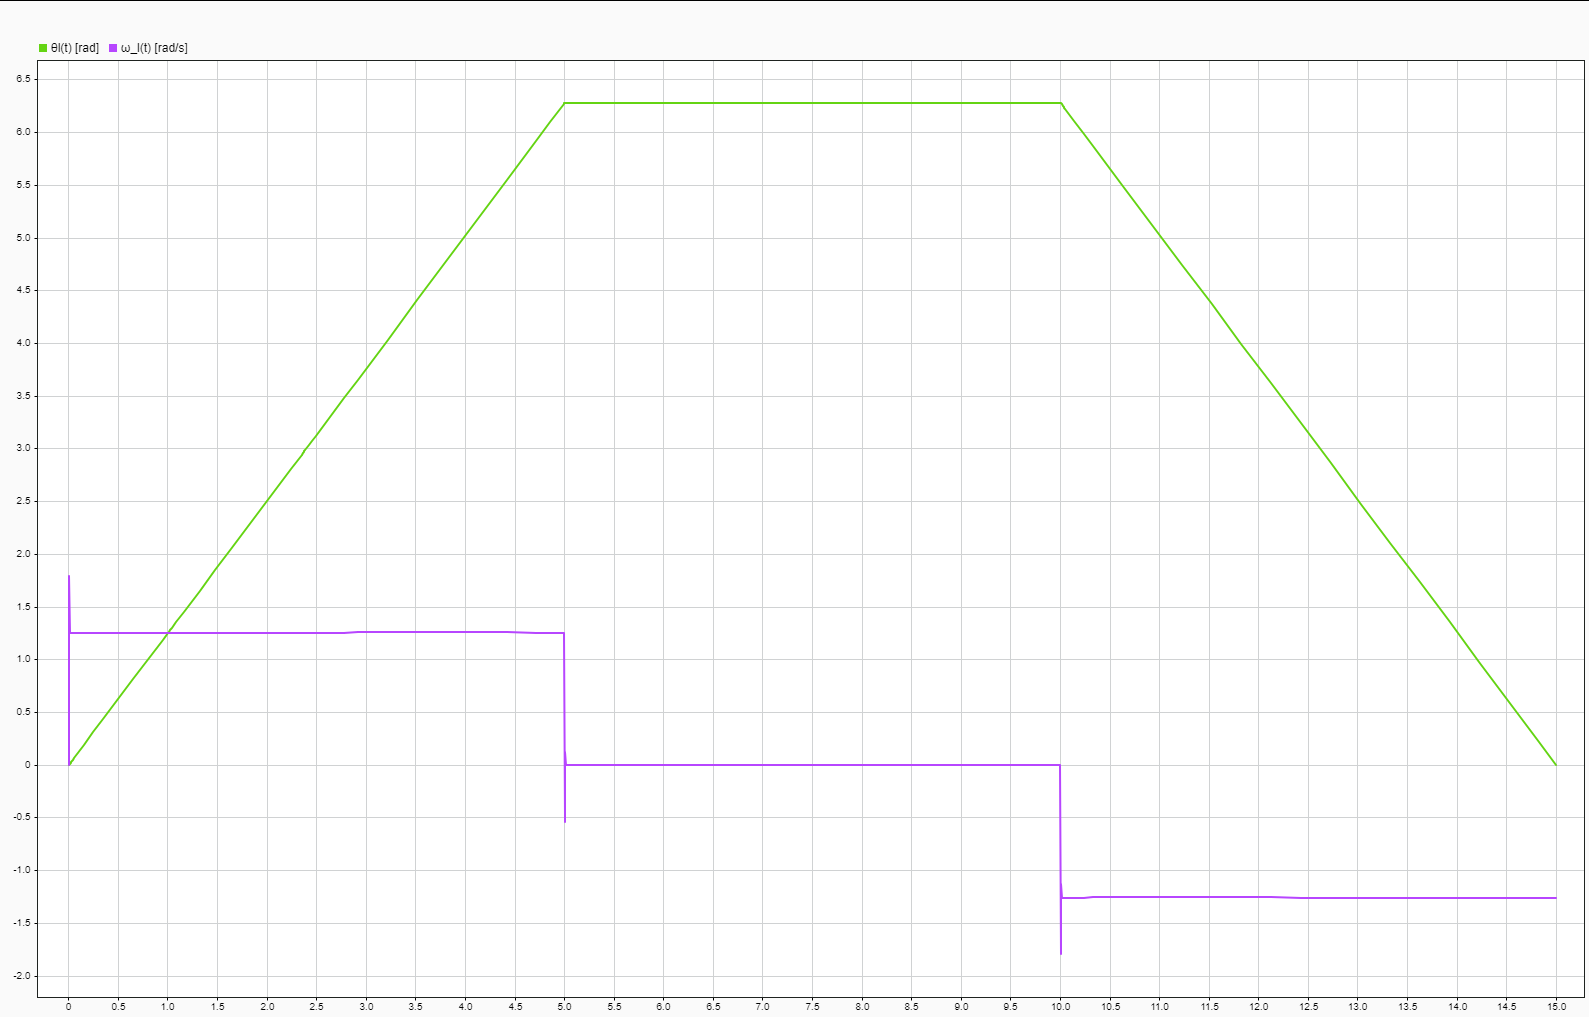
\includegraphics[width=1\linewidth]{imagenes/pos-velocidad-simulacion_cont.png}
        \caption{Posición y velocidad de la articulación en función del tiempo siguiendo la consigna trapezoidal propuesta}
    \end{figure}
    \begin{figure}[H]
        \centering
        
\includegraphics[width=1\linewidth]{imagenes/overshoot_transitorio_trap_pos.png}
        \caption{Overshoot del transitorio rampa-meseta de la posición de la articulación}
    \end{figure}
    \begin{figure}[H]
        \centering
        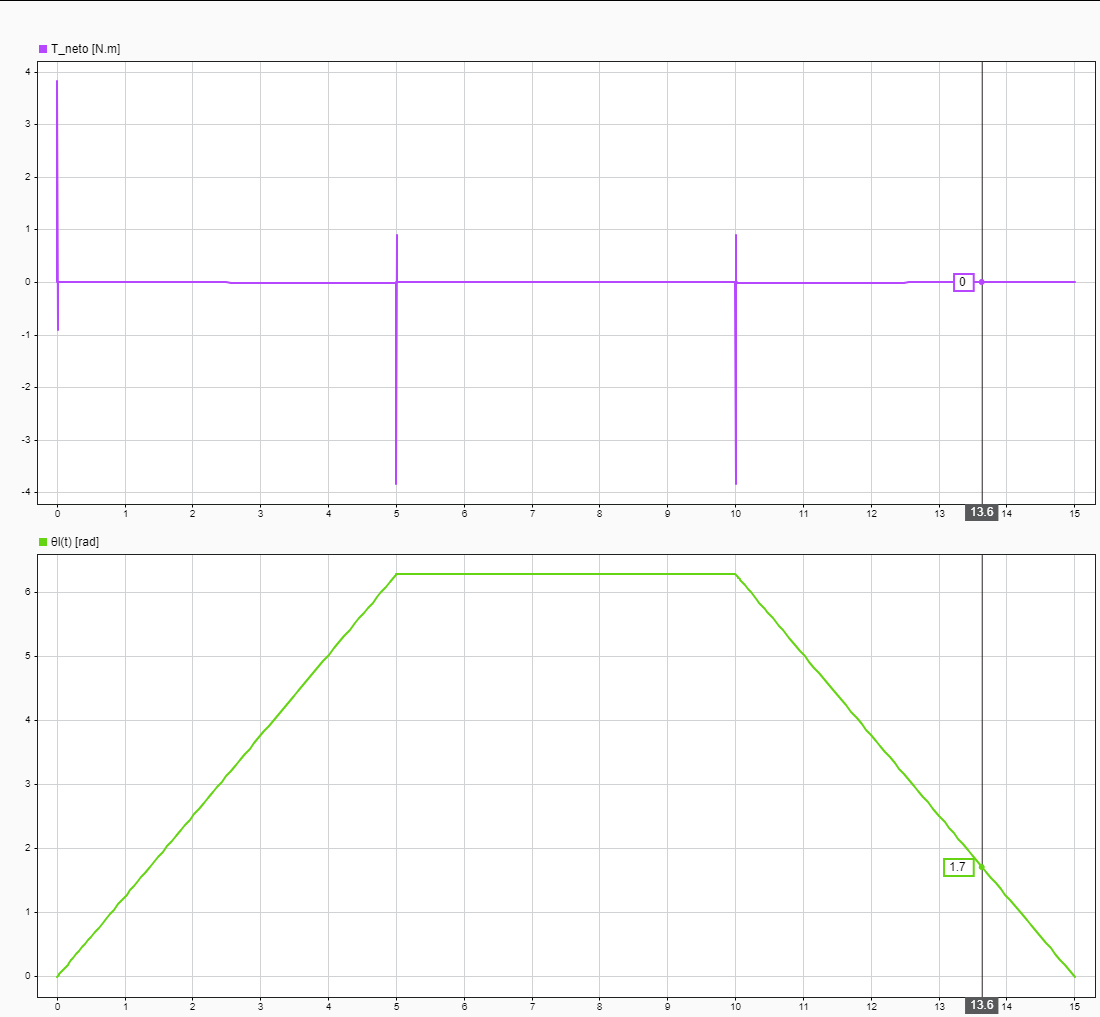
\includegraphics[width=1\linewidth]{imagenes/torque_pos_relacion.png}
        \caption{Torque neto aplicado por la articulación para seguir la consigna de posición.}
    \end{figure}
Podemos concluir a través de las distintas gráficas que el sistema sigue la consigna de forma esperada. Aun así, todavía quedan problemas que solucionar, como por ejemplo, los picos de corriente que se producen en los transitorios.
\begin{figure}[H]
    \centering
    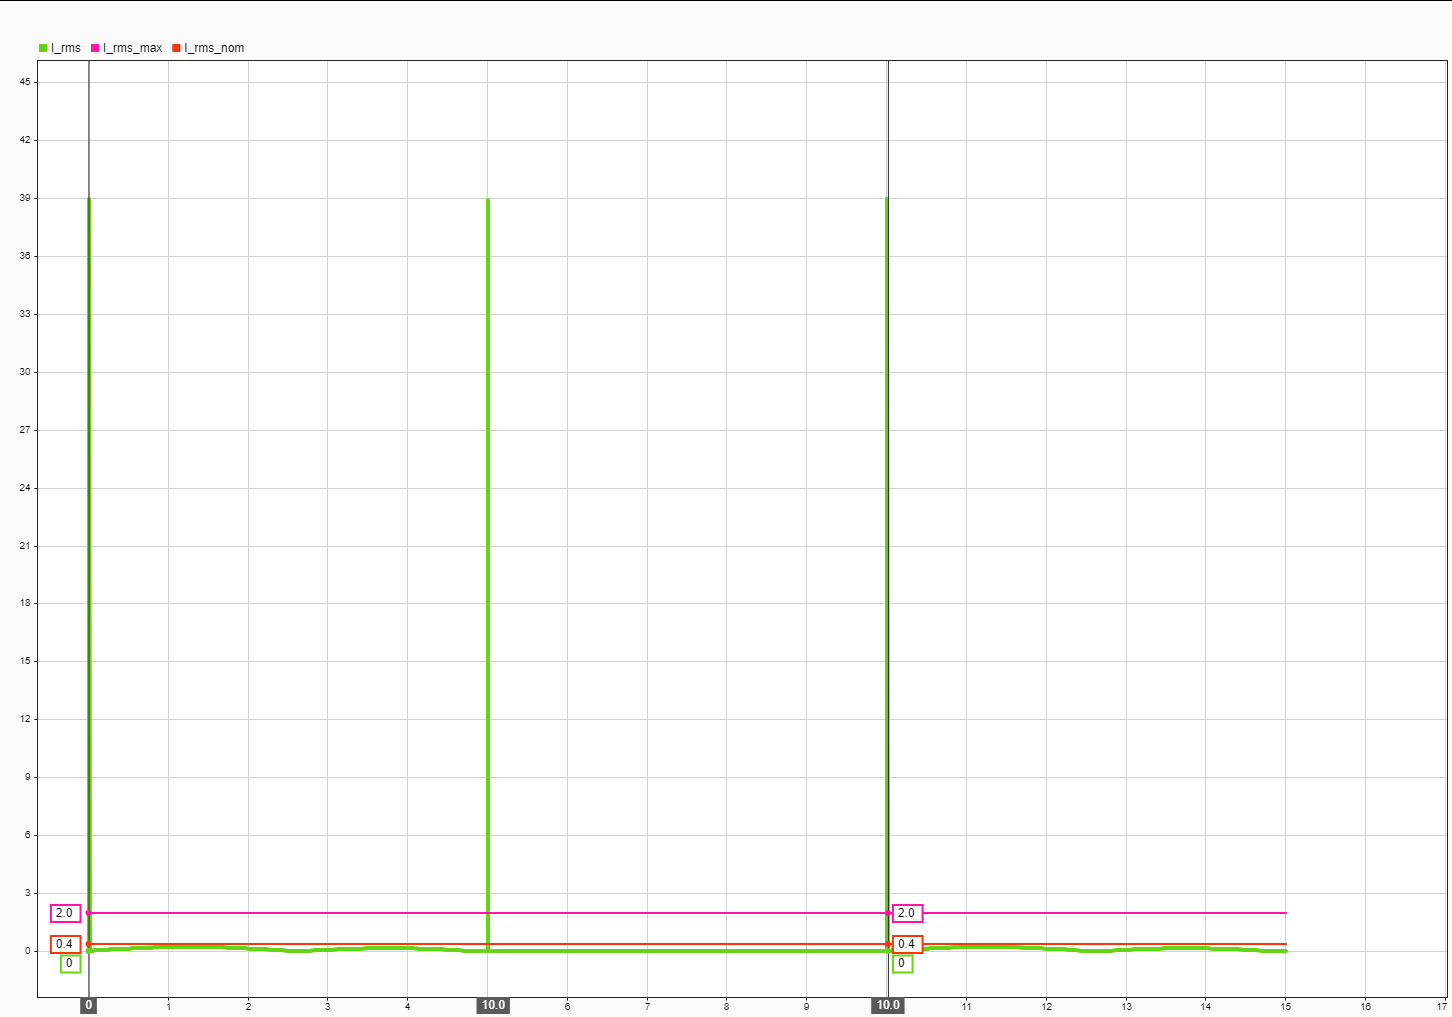
\includegraphics[width=1\linewidth]{imagenes/picos_corriente_trapz_pos.png}
    \caption{Picos de corriente rms en transitorios.}
\end{figure}
\subsubsection{Rechazo a perturbaciones $T_{ld}$ en escalón}
Se eligió una combinación de escalones para hacer más evidente el efecto del torque de perturbación y el desempeño del controlador al seguir la consigna de posición.
\[
T_{ld}(t)=
\begin{cases}
0 \ \ \text{[N.m]}, & 0 \le t < 1,\\[4pt]
5 \ \ \text{[N.m]}, & 1 \le t < 2,\\[4pt]
2{,}5 \ \ \text{[N.m]}, & 2 \le t < 3,\\[4pt]
-2{,}5 \ \ \text{[N.m]}, & 3 \le t < 5,\\[4pt]
-5 \ \ \text{[N.m]}, & 5 \le t < 6,\\[4pt]
2{,}5 \ \ \text{[N.m]}, & 6 \le t \le 15.
\end{cases}
\]

\begin{figure}[H]
    \centering
    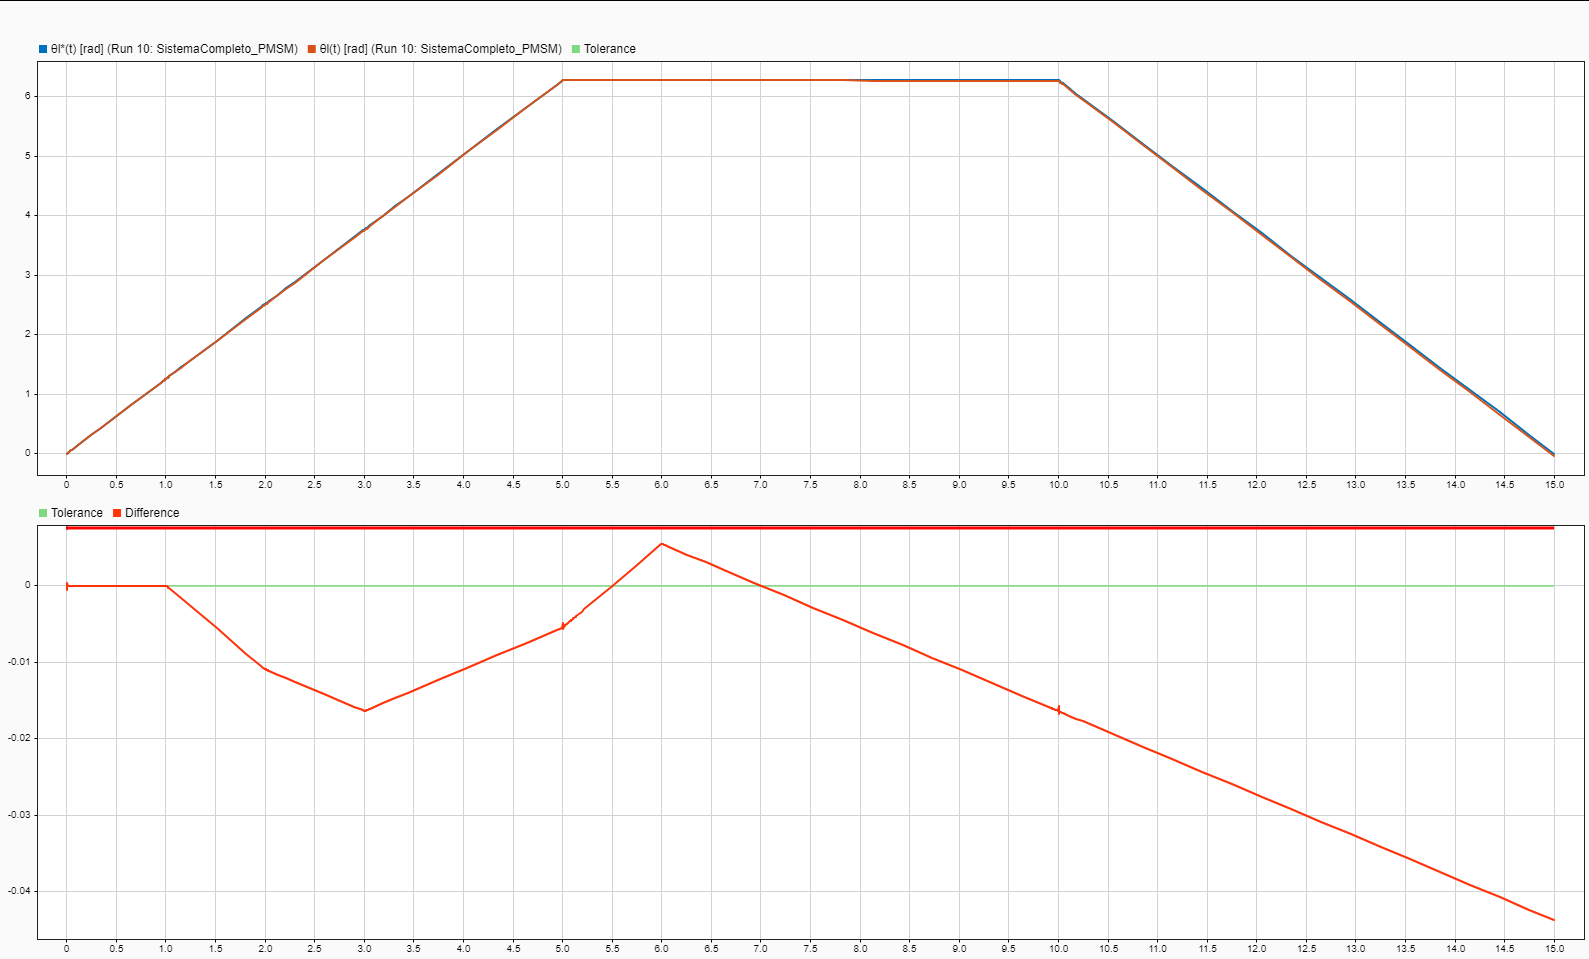
\includegraphics[width=0.75\linewidth]{imagenes/plot_perturb_error.png}
    \caption{Influencia del torque de perturbación en el seguimiento de la consigna de posición y el error creciente.}
\end{figure}
\begin{figure}[H]
    \centering
    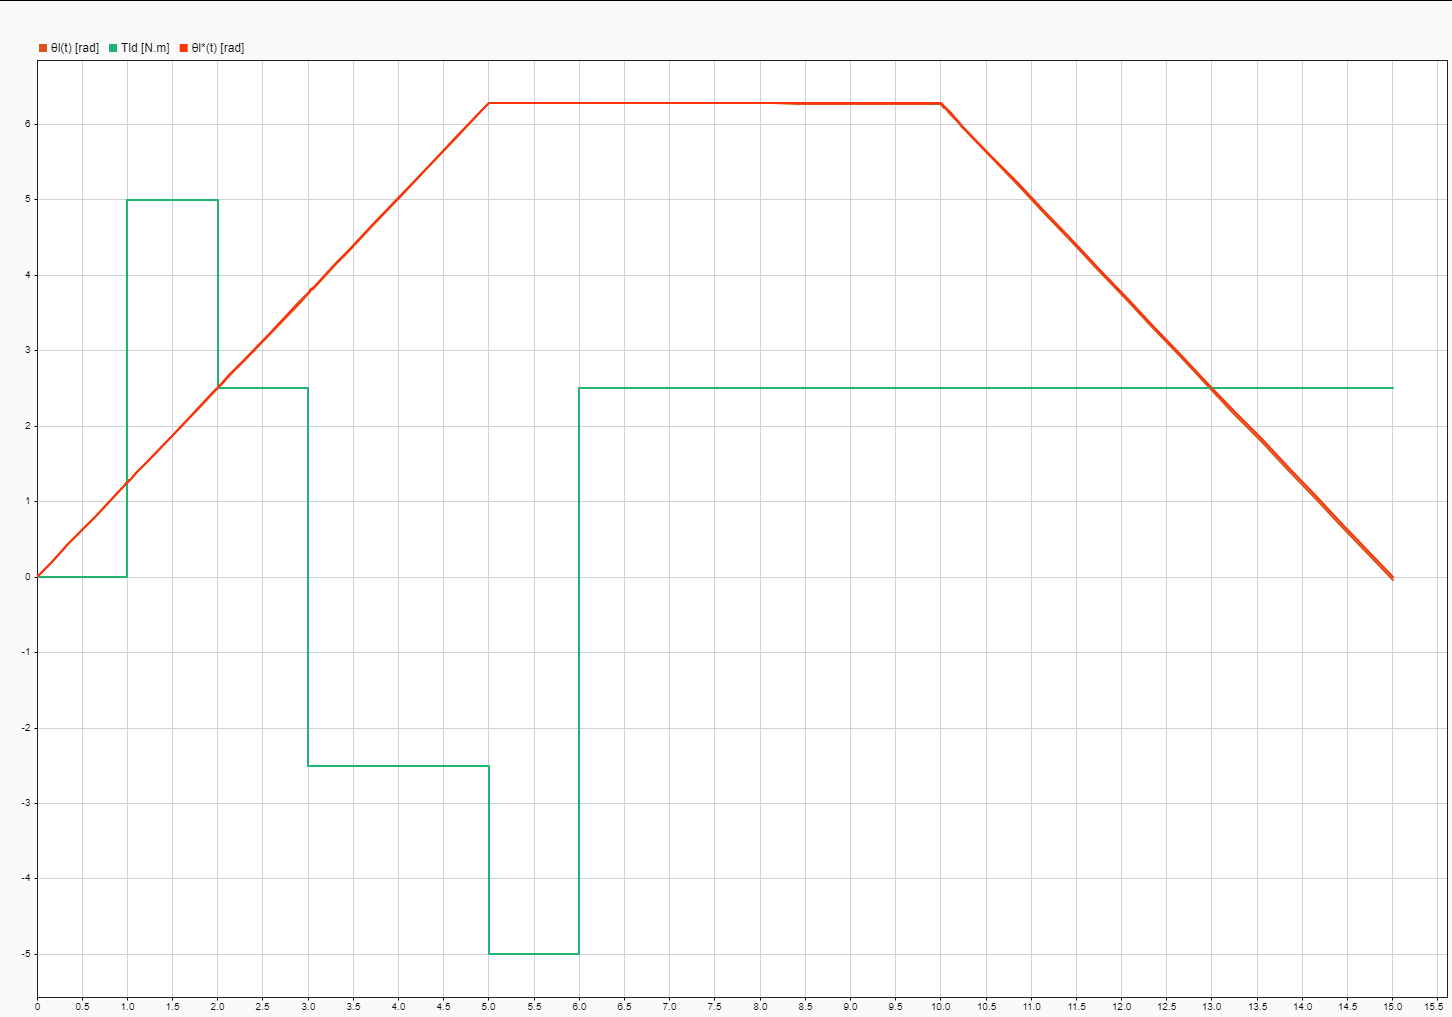
\includegraphics[width=0.75\linewidth]{imagenes/perturb_y_posicion_plot.png}
    \caption{Perturbación, consigna y posición medida. Puede verse claramente el error que aumenta con el tiempo.}
\end{figure}

\section{Verificación de desempeño y especificaciones de operación}
La primera variable que puede apreciarse que supera los límites de operación es la corriente. Para limitar este estado del sistema, primero se implementa una saturación en la tensión requerida al inversor. Para que esta no supere la especificación, debe imponerse la siguiente condición:
\begin{equation*}
\begin{aligned}
    |v_{as}(t)|,|v_{bs}(t)|,|v_{cs}(t)|\le \frac{\sqrt{2}\cdot V_{sl,max}}{\sqrt{3}}, \qquad V_{sl,max}=48\ \text{Vca rms}\\
    |v_{as}(t)|,|v_{bs}(t)|,|v_{cs}(t)|\le \frac{\sqrt{2}\cdot 48}{\sqrt{3}} = 39{,}19 \ V
    \end{aligned}
\end{equation*}
\begin{figure}[H]
    \centering
    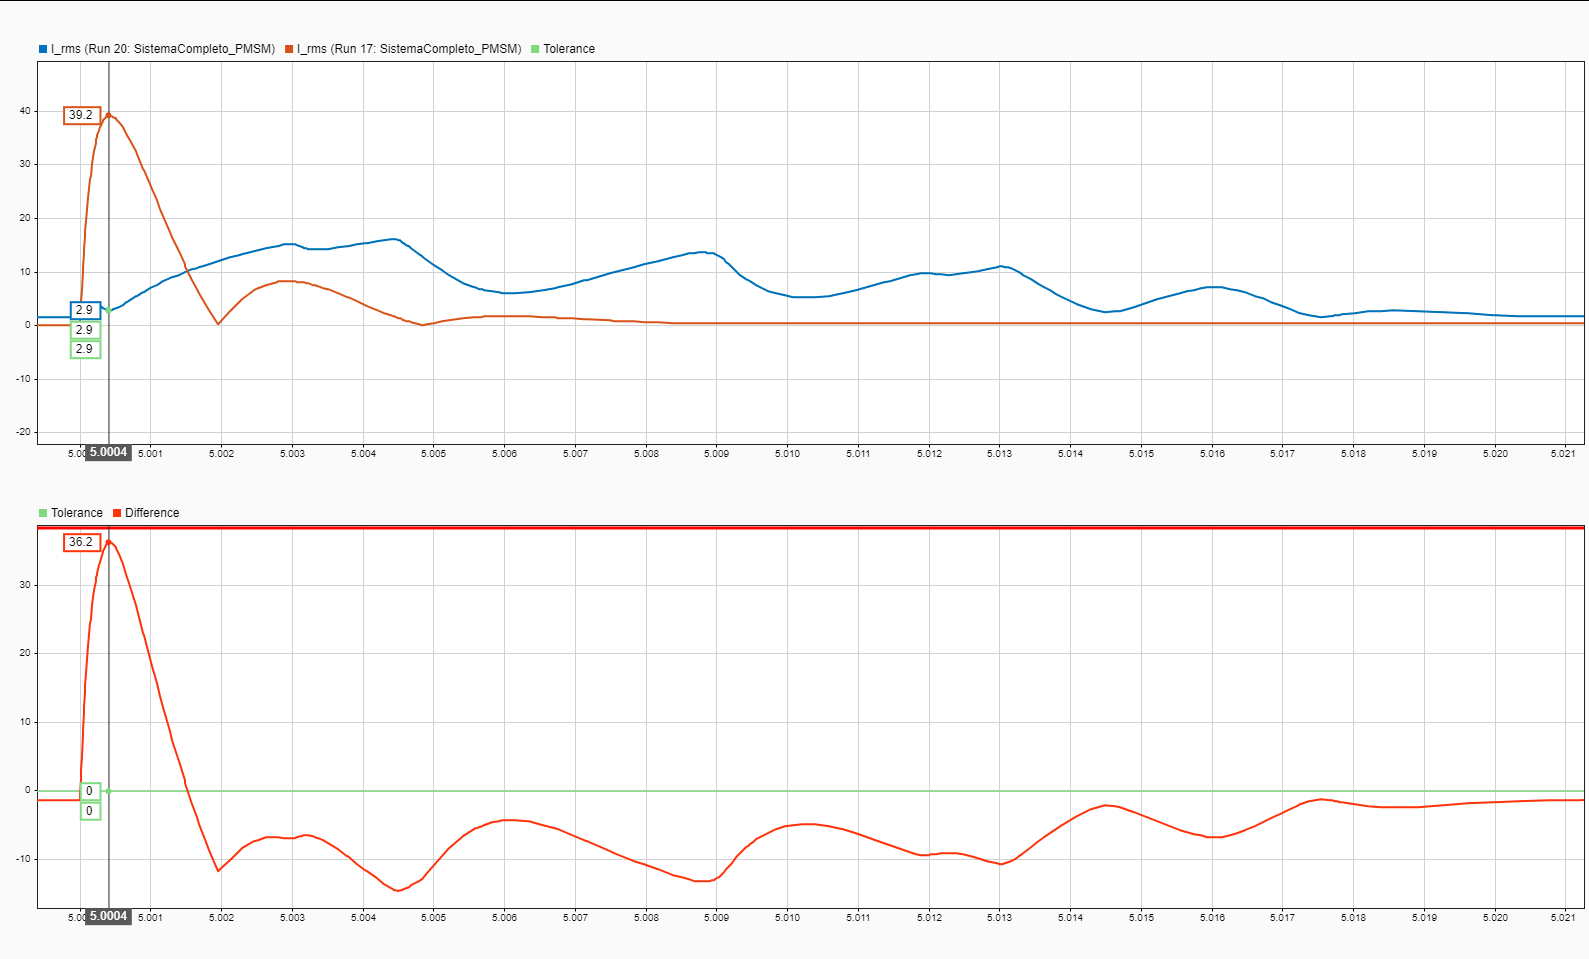
\includegraphics[width=1\linewidth]{imagenes/corrientes_limitando_voltaje.png}
    \caption{Comparación de la corriente rms del estator con y sin limitación de la tensión del inversor.}
    \label{fig:corrientes_voltaje}
\end{figure}
\begin{figure}[H]
    \centering
    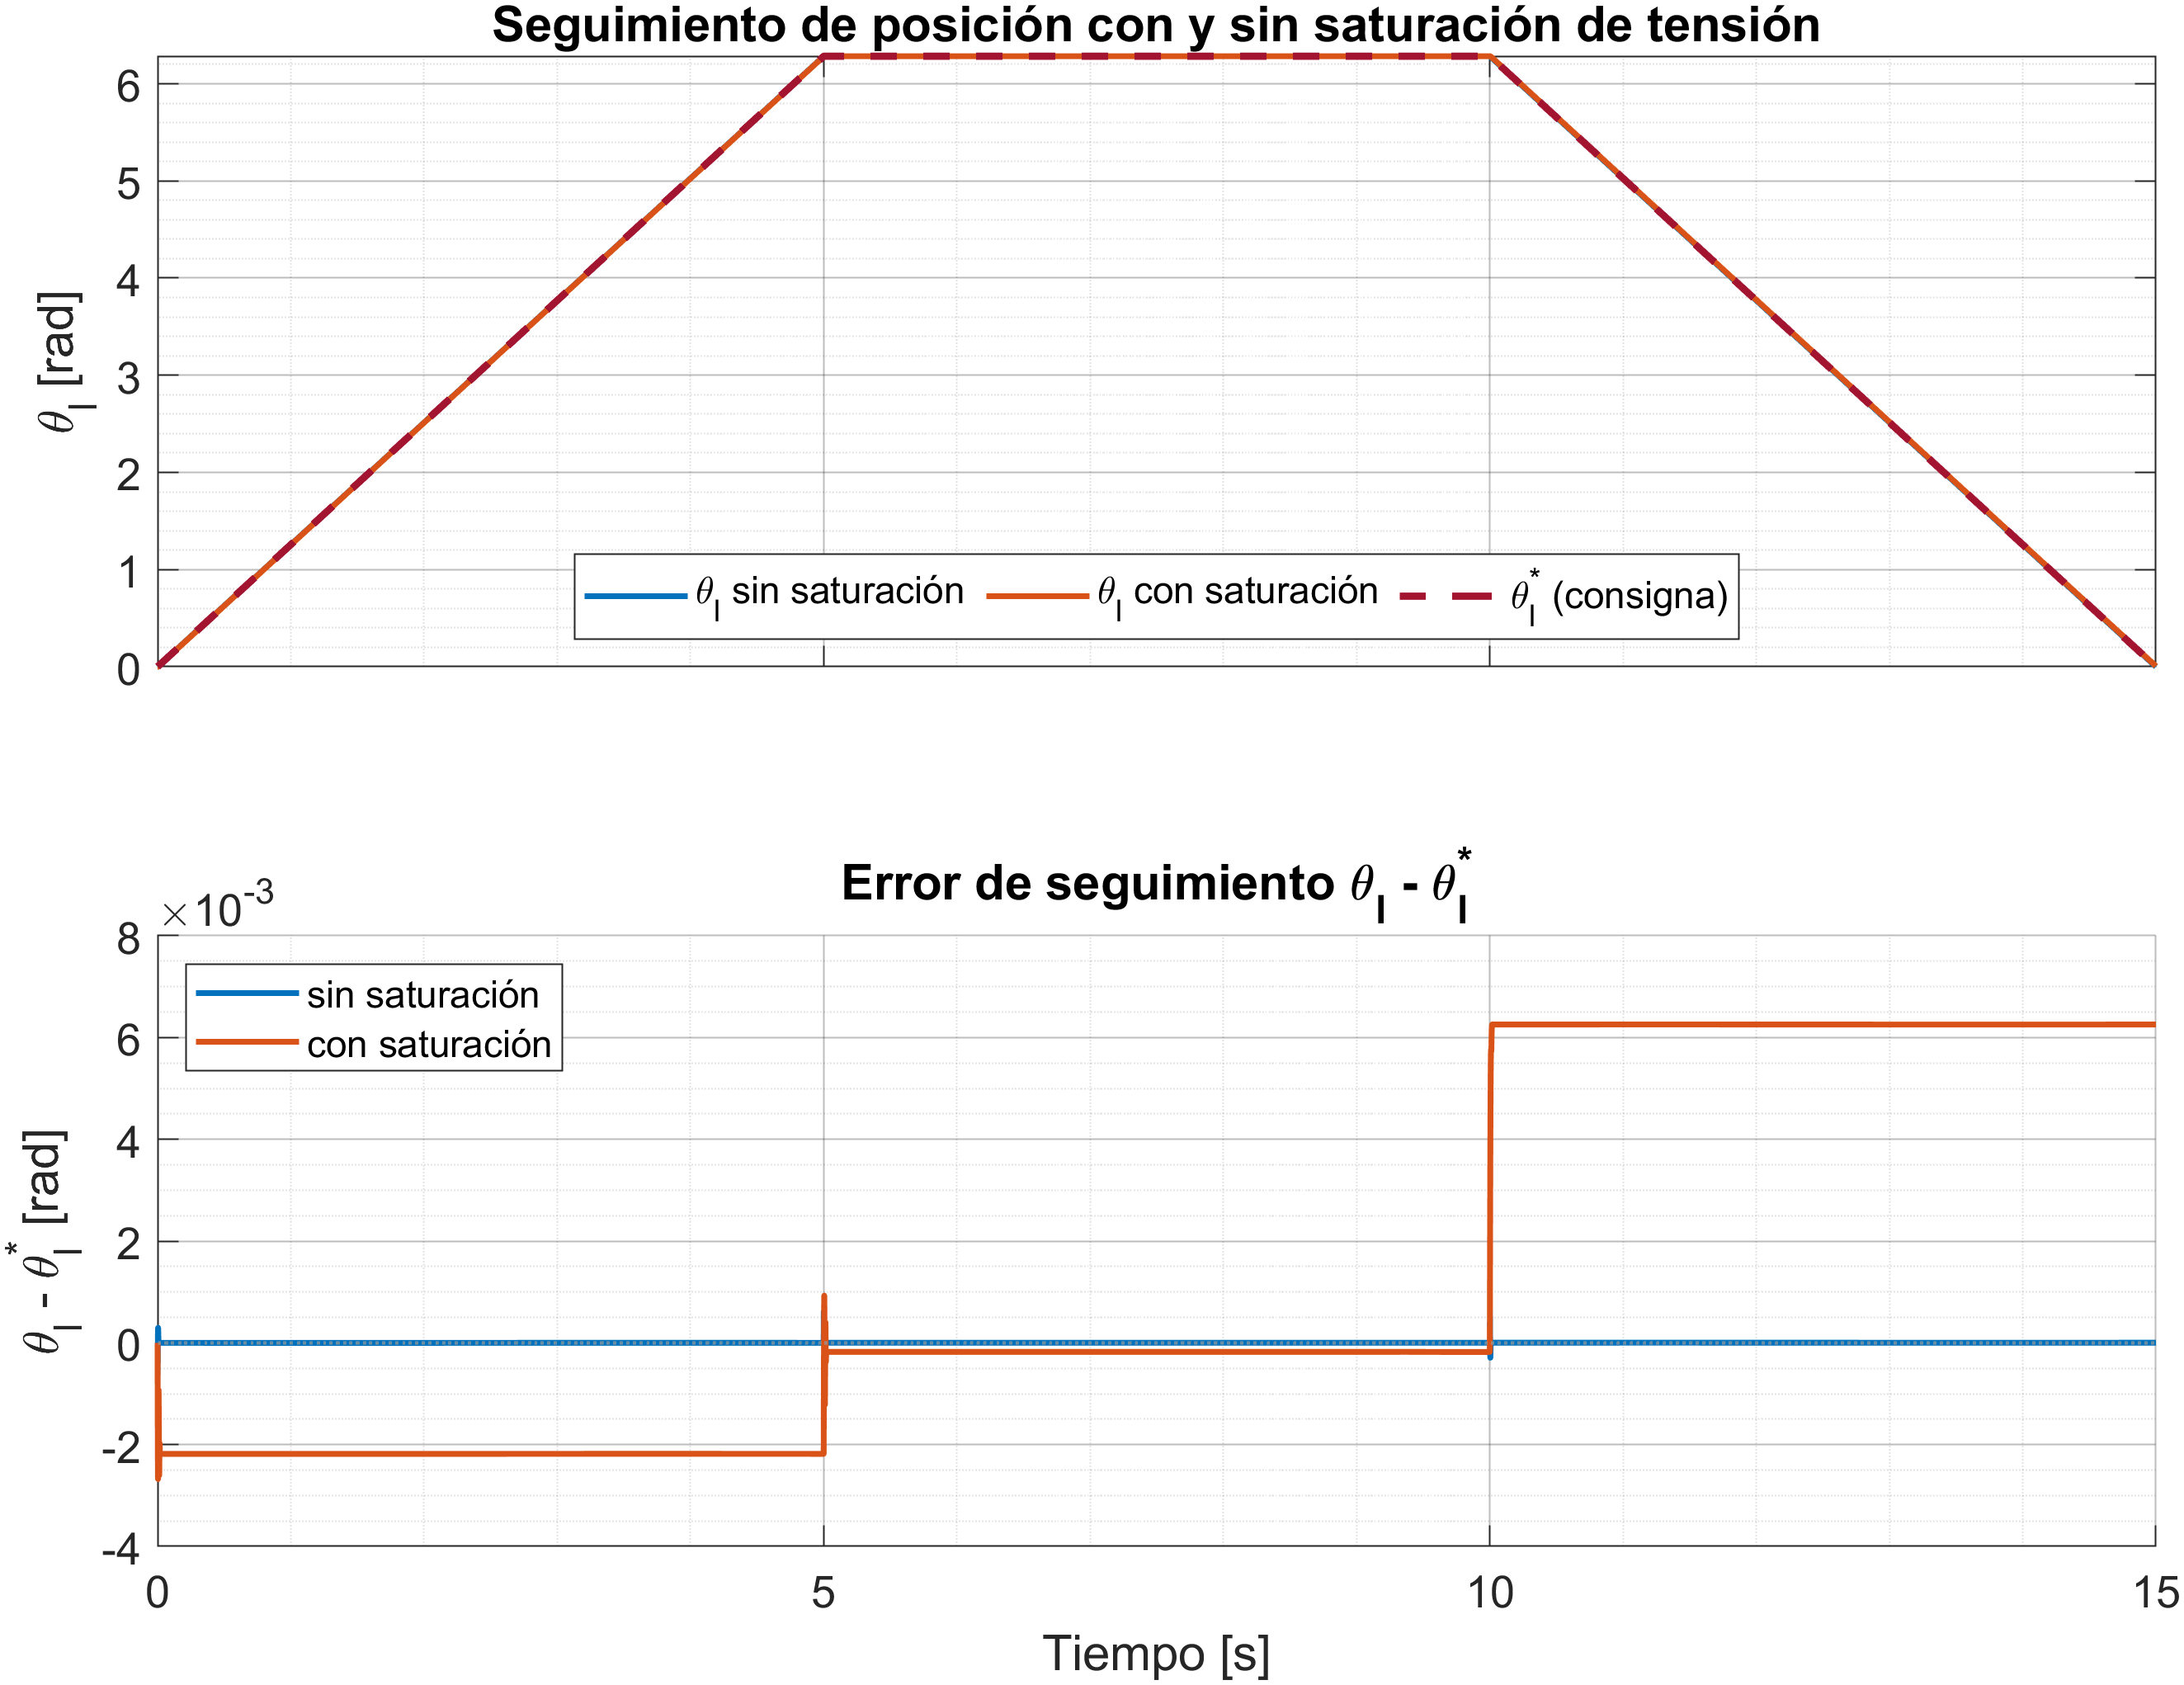
\includegraphics[width=1\linewidth]{imagenes/pos_voltaje_comparacion.png}
    \caption{Seguimiento de posición con y sin saturación de tensión del inversor ($39{,}19$~V). El seguimiento es prácticamente idéntico en ambos casos; el error de posición se mantiene en el orden de $10^{-3}$~rad.}
\end{figure}
Como puede verse en la Fig.~\ref{fig:corrientes_voltaje}, aunque se reduce bastante el tamaño del pico de corriente y el error de posición se mantiene despreciable (del orden de $10^{-3}$~rad) en la simulación con tensión saturada, esto no es suficiente para cumplir con las especificaciones de corriente.
Posteriormente se propone saturar la consigna de corriente en el modulador de torque, para que al menos no se imponga una corriente que desde un principio supere la corriente pico del motor.
\begin{figure}[H]
    \centering
    
\includegraphics[width=1\linewidth]{imagenes/corrientes_comparacion.png}
    \caption{Puede verse que, aun con saturación en la consigna de corriente, el accionamiento no puede cumplir la consigna sin superar sus especificaciones.}
\end{figure}
Finalmente, esto lleva a modificar la forma de la consigna. Si se analizan las gráficas previas de la simulación, puede verse que por momentos se solicitan aceleraciones infinitas al accionamiento (saltos discontinuos en la velocidad).

Inicialmente se propuso implementar un perfil trapezoidal de velocidad, obteniendo resultados sustancialmente superiores en términos de cumplimiento de especificaciones.
\begin{figure}[H]
    \centering
    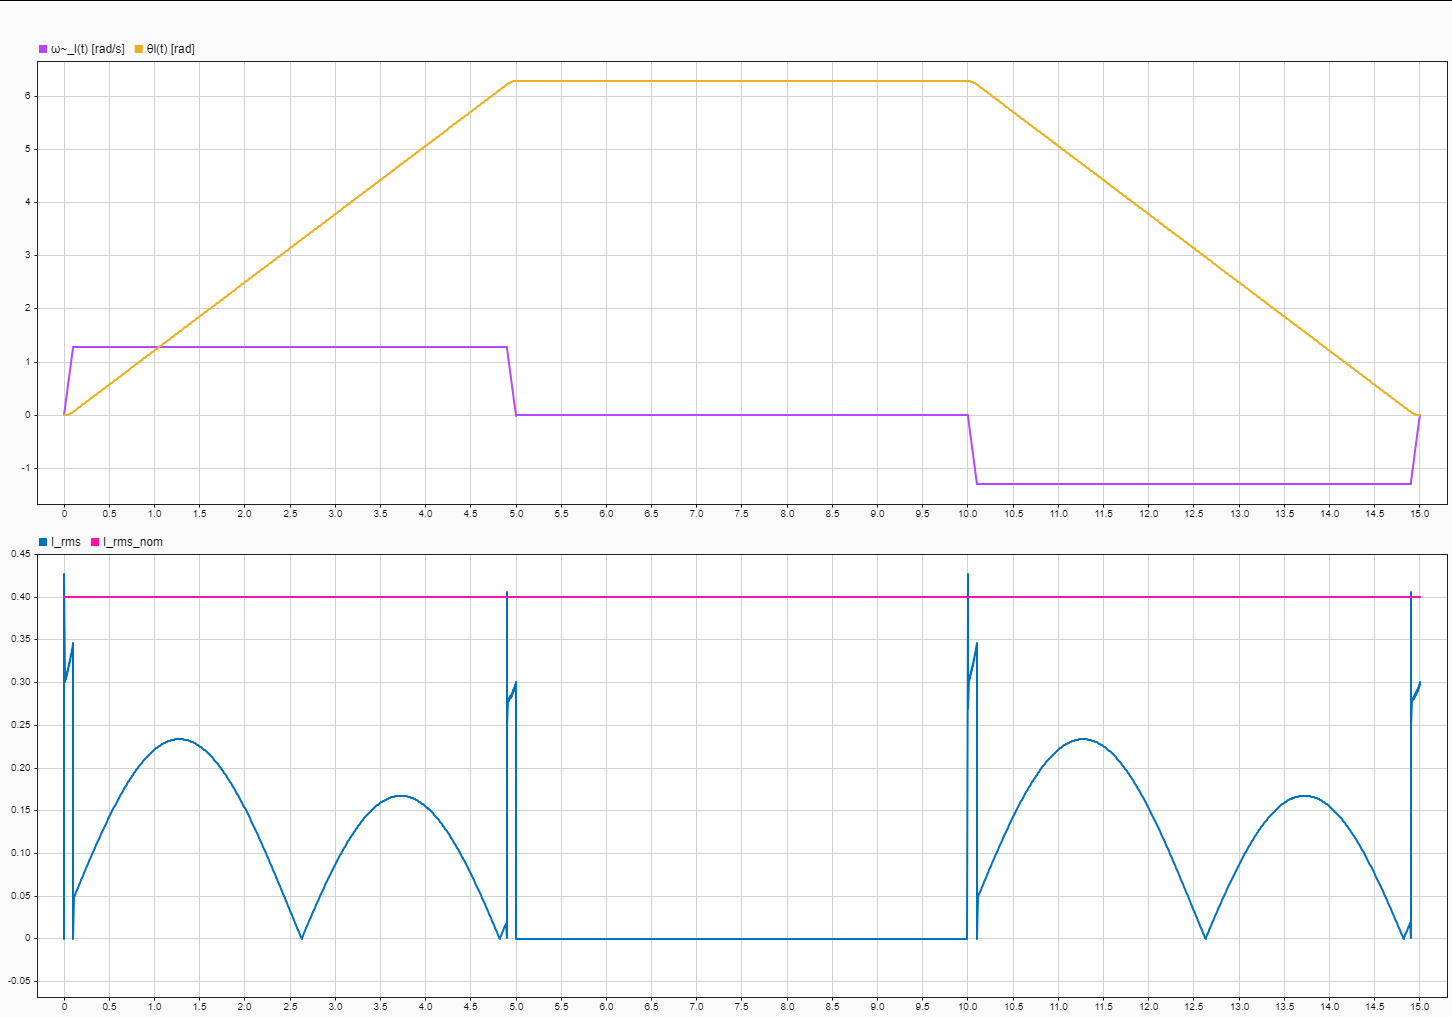
\includegraphics[width=0.75\linewidth]{imagenes/perfil_trap_vel_comp.png}
    \caption{En este caso, con un tiempo de rampa de $t=0{,}1$~s, puede verse que la corriente pico apenas supera los $0{,}4$~A.}
\end{figure}
El perfil de velocidad se desarrolló implementando un generador de trayectorias; es decir, se permite ingresar una \textit{matriz de consigna de posición} y luego, mediante un bloque MATLAB Function, se vectoriza el vector de tiempo y de puntos en el espacio. Se presentan más detalles en el Anexo~\ref{anexo:gen_trayectorias}.
Como era de esperarse, aunque la implementación del perfil de velocidad trapezoidal corrigió en buena medida el problema, las discontinuidades en la corriente y, por lo tanto, en la aceleración, producían \textit{jerk} infinito, lo que en una articulación real sería inaceptable. Por este motivo, se extendió el generador de trayectorias a la generación de un perfil trapezoidal de aceleración, obteniendo el siguiente resultado.
\begin{figure}[H]
    \centering
    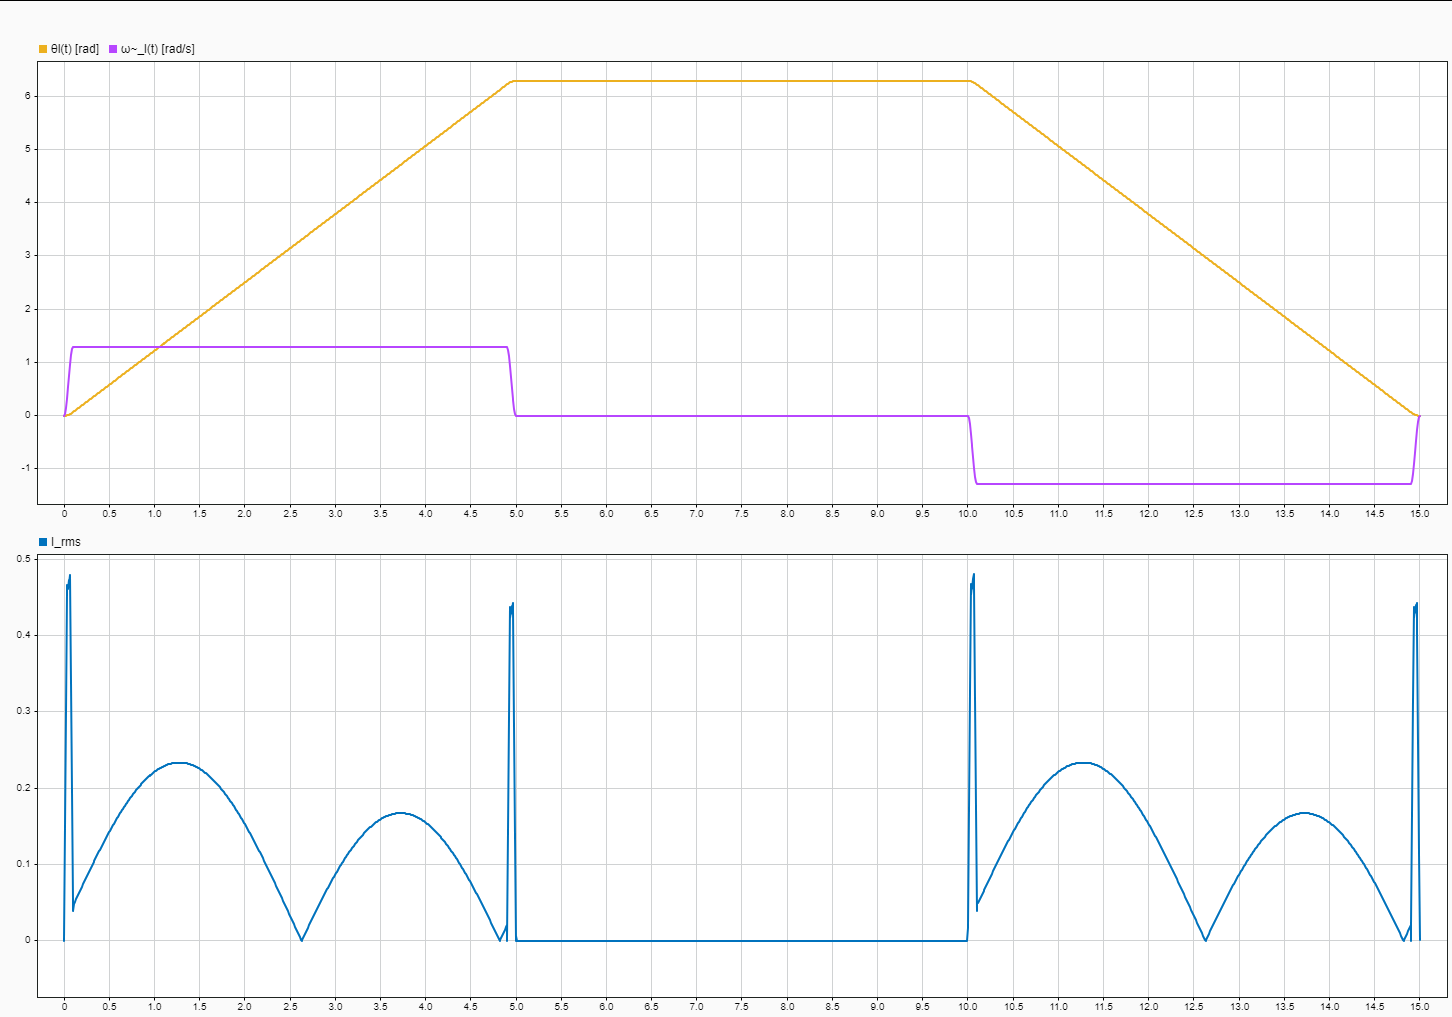
\includegraphics[width=1\linewidth]{imagenes/perfil_trap_accel_comp.png}
    \caption{Eliminación de los picos no derivables de corriente y aceleración.}
\end{figure}

\subsection{Mejora del observador mecánico ante perturbaciones constantes}

El observador mecánico implementado originalmente responde a la estructura clásica de Luenberger para el subsistema mecánico simplificado, utilizando como variable medida la posición angular del eje del motor $\theta_m(t)$ y reconstruyendo la velocidad angular $\omega_m(t)$ a partir del modelo y del error de salida. Dado que la consigna establece ubicar los polos del observador en
\[
p_{obs\,1,2}=-3200\ \text{rad/s},
\]
se adoptó inicialmente el observador de segundo orden como diseño base.

Partiendo del modelo mecánico simplificado utilizado para el diseño,
\begin{equation}
\dot{\theta}_m(t)=\omega_m(t), 
\qquad
\dot{\omega}_m(t)=\frac{1}{J_{eq}}\,T_m'(t),
\end{equation}
y definiendo la salida medida como
\begin{equation}
y(t)=\theta_m(t),
\end{equation}
el observador base queda dado por:
\begin{equation}
\label{eq:obs_base}
\begin{aligned}
    \dot{\hat{\theta}}_m(t) &= \hat{\omega}_m(t) + K_{e\theta_m}\big(\theta_m(t)-\hat{\theta}_m(t)\big), \\
    \dot{\hat{\omega}}_m(t) &= \frac{1}{J_{eq}}\,T_m'(t) + K_{e\omega_m}\big(\theta_m(t)-\hat{\theta}_m(t)\big).
\end{aligned}
\end{equation}

Definiendo el error de estimación como
\begin{equation}
e_\theta(t)=\theta_m(t)-\hat{\theta}_m(t),
\qquad
e_\omega(t)=\omega_m(t)-\hat{\omega}_m(t),
\end{equation}
la dinámica del error para el observador base queda:
\begin{equation}
\begin{bmatrix}
\dot e_\theta(t)\\
\dot e_\omega(t)
\end{bmatrix}
=
\begin{bmatrix}
-K_{e\theta_m} & 1\\
-K_{e\omega_m} & 0
\end{bmatrix}
\begin{bmatrix}
e_\theta(t)\\
e_\omega(t)
\end{bmatrix}.
\end{equation}

Por lo tanto, el polinomio característico asociado es
\begin{equation}
p_{obs}(s)=s^2+K_{e\theta_m}s+K_{e\omega_m}.
\end{equation}

Imponiendo como polinomio deseado
\begin{equation}
p_{des}(s)=(s+3200)^2=s^2+6400\,s+3200^2,
\end{equation}
se obtienen las ganancias del observador base:
\begin{equation}
\label{eq:ganancias_obs_base}
K_{e\theta_m}=6400\ \mathrm{s}^{-1},
\qquad
K_{e\omega_m}=3200^2=1{,}024\times10^7\ \mathrm{s}^{-2}.
\end{equation}

Con estas ganancias, el observador reconstruye adecuadamente la velocidad en transitorios y presenta una rapidez de convergencia suficientemente mayor que la dinámica dominante del controlador externo. No obstante, en la verificación de desempeño se observa que ante perturbaciones de carga cuasi-estacionarias aparece un error de estimación de régimen permanente distinto de cero. Esto indica que, aunque el observador base es estable y rápido, no rechaza completamente perturbaciones constantes o pequeños sesgos de modelado.

\begin{figure}[H]
    \centering
    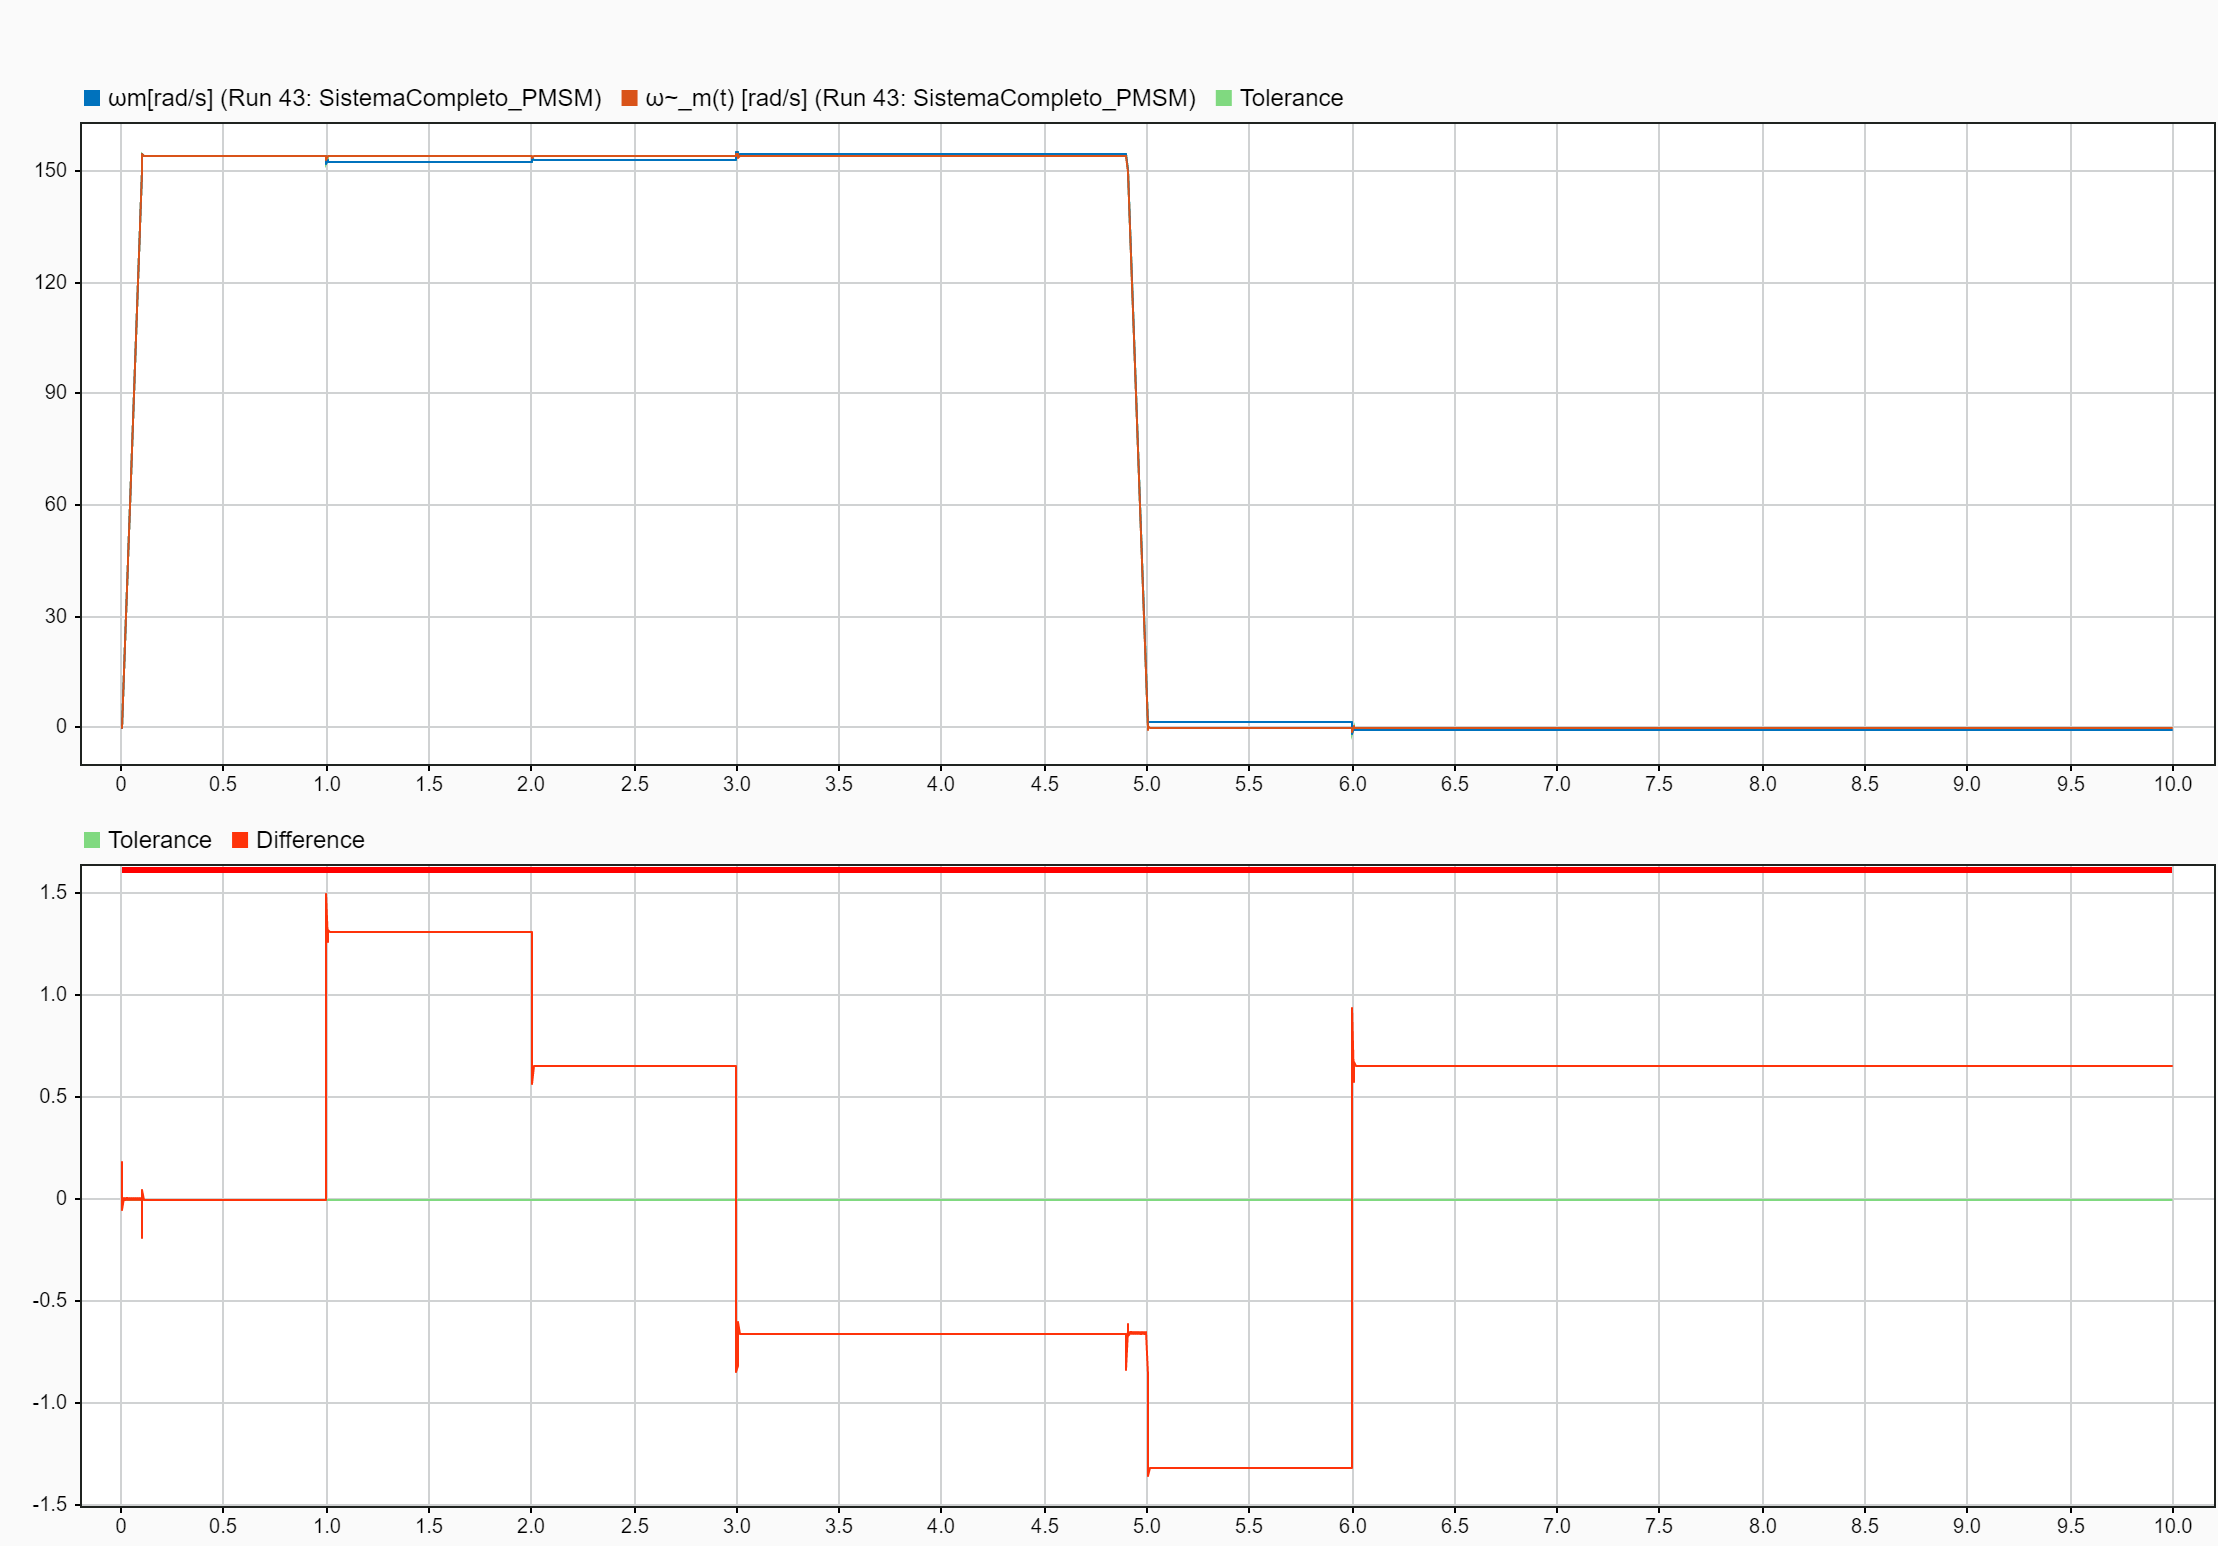
\includegraphics[width=0.78\linewidth]{imagenes/5_2_5_B_error_observador.png}
    \caption{Error de offset observado con el observador mecánico de segundo orden sin acción integral, ante perturbaciones de carga cuasi-estacionarias.}
    \label{fig:obs_offset_original}
\end{figure}

En consecuencia, el observador de segundo orden se conserva como paso intermedio de diseño, pero no como solución definitiva. Para eliminar este offset se propone aumentar el observador con una acción integral del error de posición.

Se define un nuevo estado auxiliar $z(t)$ como:
\begin{equation}
\label{eq:def_z_obs}
e_{\theta}(t)=\theta_m(t)-\hat{\theta}_m(t),
\qquad
\dot z(t)=e_{\theta}(t).
\end{equation}

De esta manera, el observador mecánico aumentado queda:
\begin{equation}
\label{eq:obs_integral}
\begin{aligned}
    \dot{\hat{\theta}}_m(t) &= \hat{\omega}_m(t) + K_{e\theta_m}\,e_{\theta}(t), \\
    \dot{\hat{\omega}}_m(t) &= \frac{1}{J_{eq}}\,T_m'(t) + K_{e\omega_m}\,e_{\theta}(t) + K_{ei_m}\,z(t), \\
    \dot z(t) &= e_{\theta}(t).
\end{aligned}
\end{equation}

En esta formulación, el término $K_{ei_m}z(t)$ introduce una corrección integral sobre el error de posición. Físicamente, esto permite compensar perturbaciones mecánicas aproximadamente constantes o incertidumbres de modelado que, en el observador base, se manifestaban como un sesgo persistente en la velocidad estimada y, por integración, también en la posición estimada.

Definiendo ahora el vector de error aumentado
\begin{equation}
\mathbf e_a(t)=
\begin{bmatrix}
e_\theta(t)\\
e_\omega(t)\\
z(t)
\end{bmatrix},
\end{equation}
la dinámica del error queda gobernada por
\begin{equation}
\dot{\mathbf e}_a(t)=
\underbrace{
\begin{bmatrix}
-K_{e\theta_m} & 1 & 0\\
-K_{e\omega_m} & 0 & -K_{ei_m}\\
1 & 0 & 0
\end{bmatrix}
}_{\mathbf A_{obs,a}}
\mathbf e_a(t),
\end{equation}
cuyo polinomio característico resulta
\begin{equation}
\label{eq:polinomio_obs_integral}
p_{obs,a}(s)=s^3+K_{e\theta_m}s^2+K_{e\omega_m}s+K_{ei_m}.
\end{equation}

Para conservar aproximadamente la misma rapidez principal de convergencia que en el observador original, se ubican los tres polos reales e iguales en:
\begin{equation}
p_{obs\,1,2,3}=-3200\ \text{rad/s}.
\end{equation}

Así, el polinomio deseado es
\begin{equation}
p_{des,a}(s)=(s+3200)^3
=s^3+9600\,s^2+3{,}072\times10^7\,s+3{,}2768\times10^{10}.
\end{equation}

Comparando coeficientes con \eqref{eq:polinomio_obs_integral}, se obtienen las ganancias del observador aumentado:
\begin{equation}
\label{eq:ganancias_obs_integral}
K_{e\theta_m}=9600\ \mathrm{s}^{-1},
\qquad
K_{e\omega_m}=3{,}072\times10^7\ \mathrm{s}^{-2},
\qquad
K_{ei_m}=3{,}2768\times10^{10}\ \mathrm{s}^{-3}.
\end{equation}

Desde el punto de vista de implementación en Simulink, esta mejora se incorpora mediante una rama adicional en paralelo:
\begin{enumerate}
    \item se calcula el error de posición $e_{\theta}(t)=\theta_m(t)-\hat{\theta}_m(t)$;

    \item dicho error alimenta un integrador $1/s$, cuya salida es el estado $z(t)$;
    \item la salida $z(t)$ se multiplica por la ganancia $K_{ei_m}$;
    \item la señal $K_{ei_m}z(t)$ se suma en la ecuación de $\dot{\hat{\omega}}_m(t)$ junto con el término de modelo y la corrección proporcional $K_{e\omega_m}e_{\theta}(t)$;
    \item la velocidad estimada $\hat{\omega}_m(t)$ se integra para obtener $\hat{\theta}_m(t)$, cerrando la realimentación del observador.
\end{enumerate}

\begin{figure}[H]
    \centering
    
\includegraphics[width=0.92\linewidth]{imagenes/5_2_5_B_diagrama_bloques_observador.png}
    \caption{Diagrama de bloques del observador mecánico aumentado con acción integral implementado en Simulink. El error de posición $e_{\theta}(t)=\theta_m(t)-\hat{\theta}_m(t)$ alimenta tanto las ramas proporcionales como la rama integral, cuya salida corrige la dinámica de $\dot{\hat{\omega}}_m(t)$ para eliminar el error estacionario de estimación.}
    \label{fig:obs_bloques_integral}
\end{figure}

En la práctica, esta estructura puede interpretarse también como una estimación implícita de una perturbación mecánica constante o de un \textit{bias} equivalente no modelado. Sin embargo, independientemente de esa interpretación física, la conclusión relevante para el presente trabajo es que la incorporación del estado integral elimina el error estacionario de estimación frente a perturbaciones constantes de carga.

\begin{figure}[H]
    \centering
    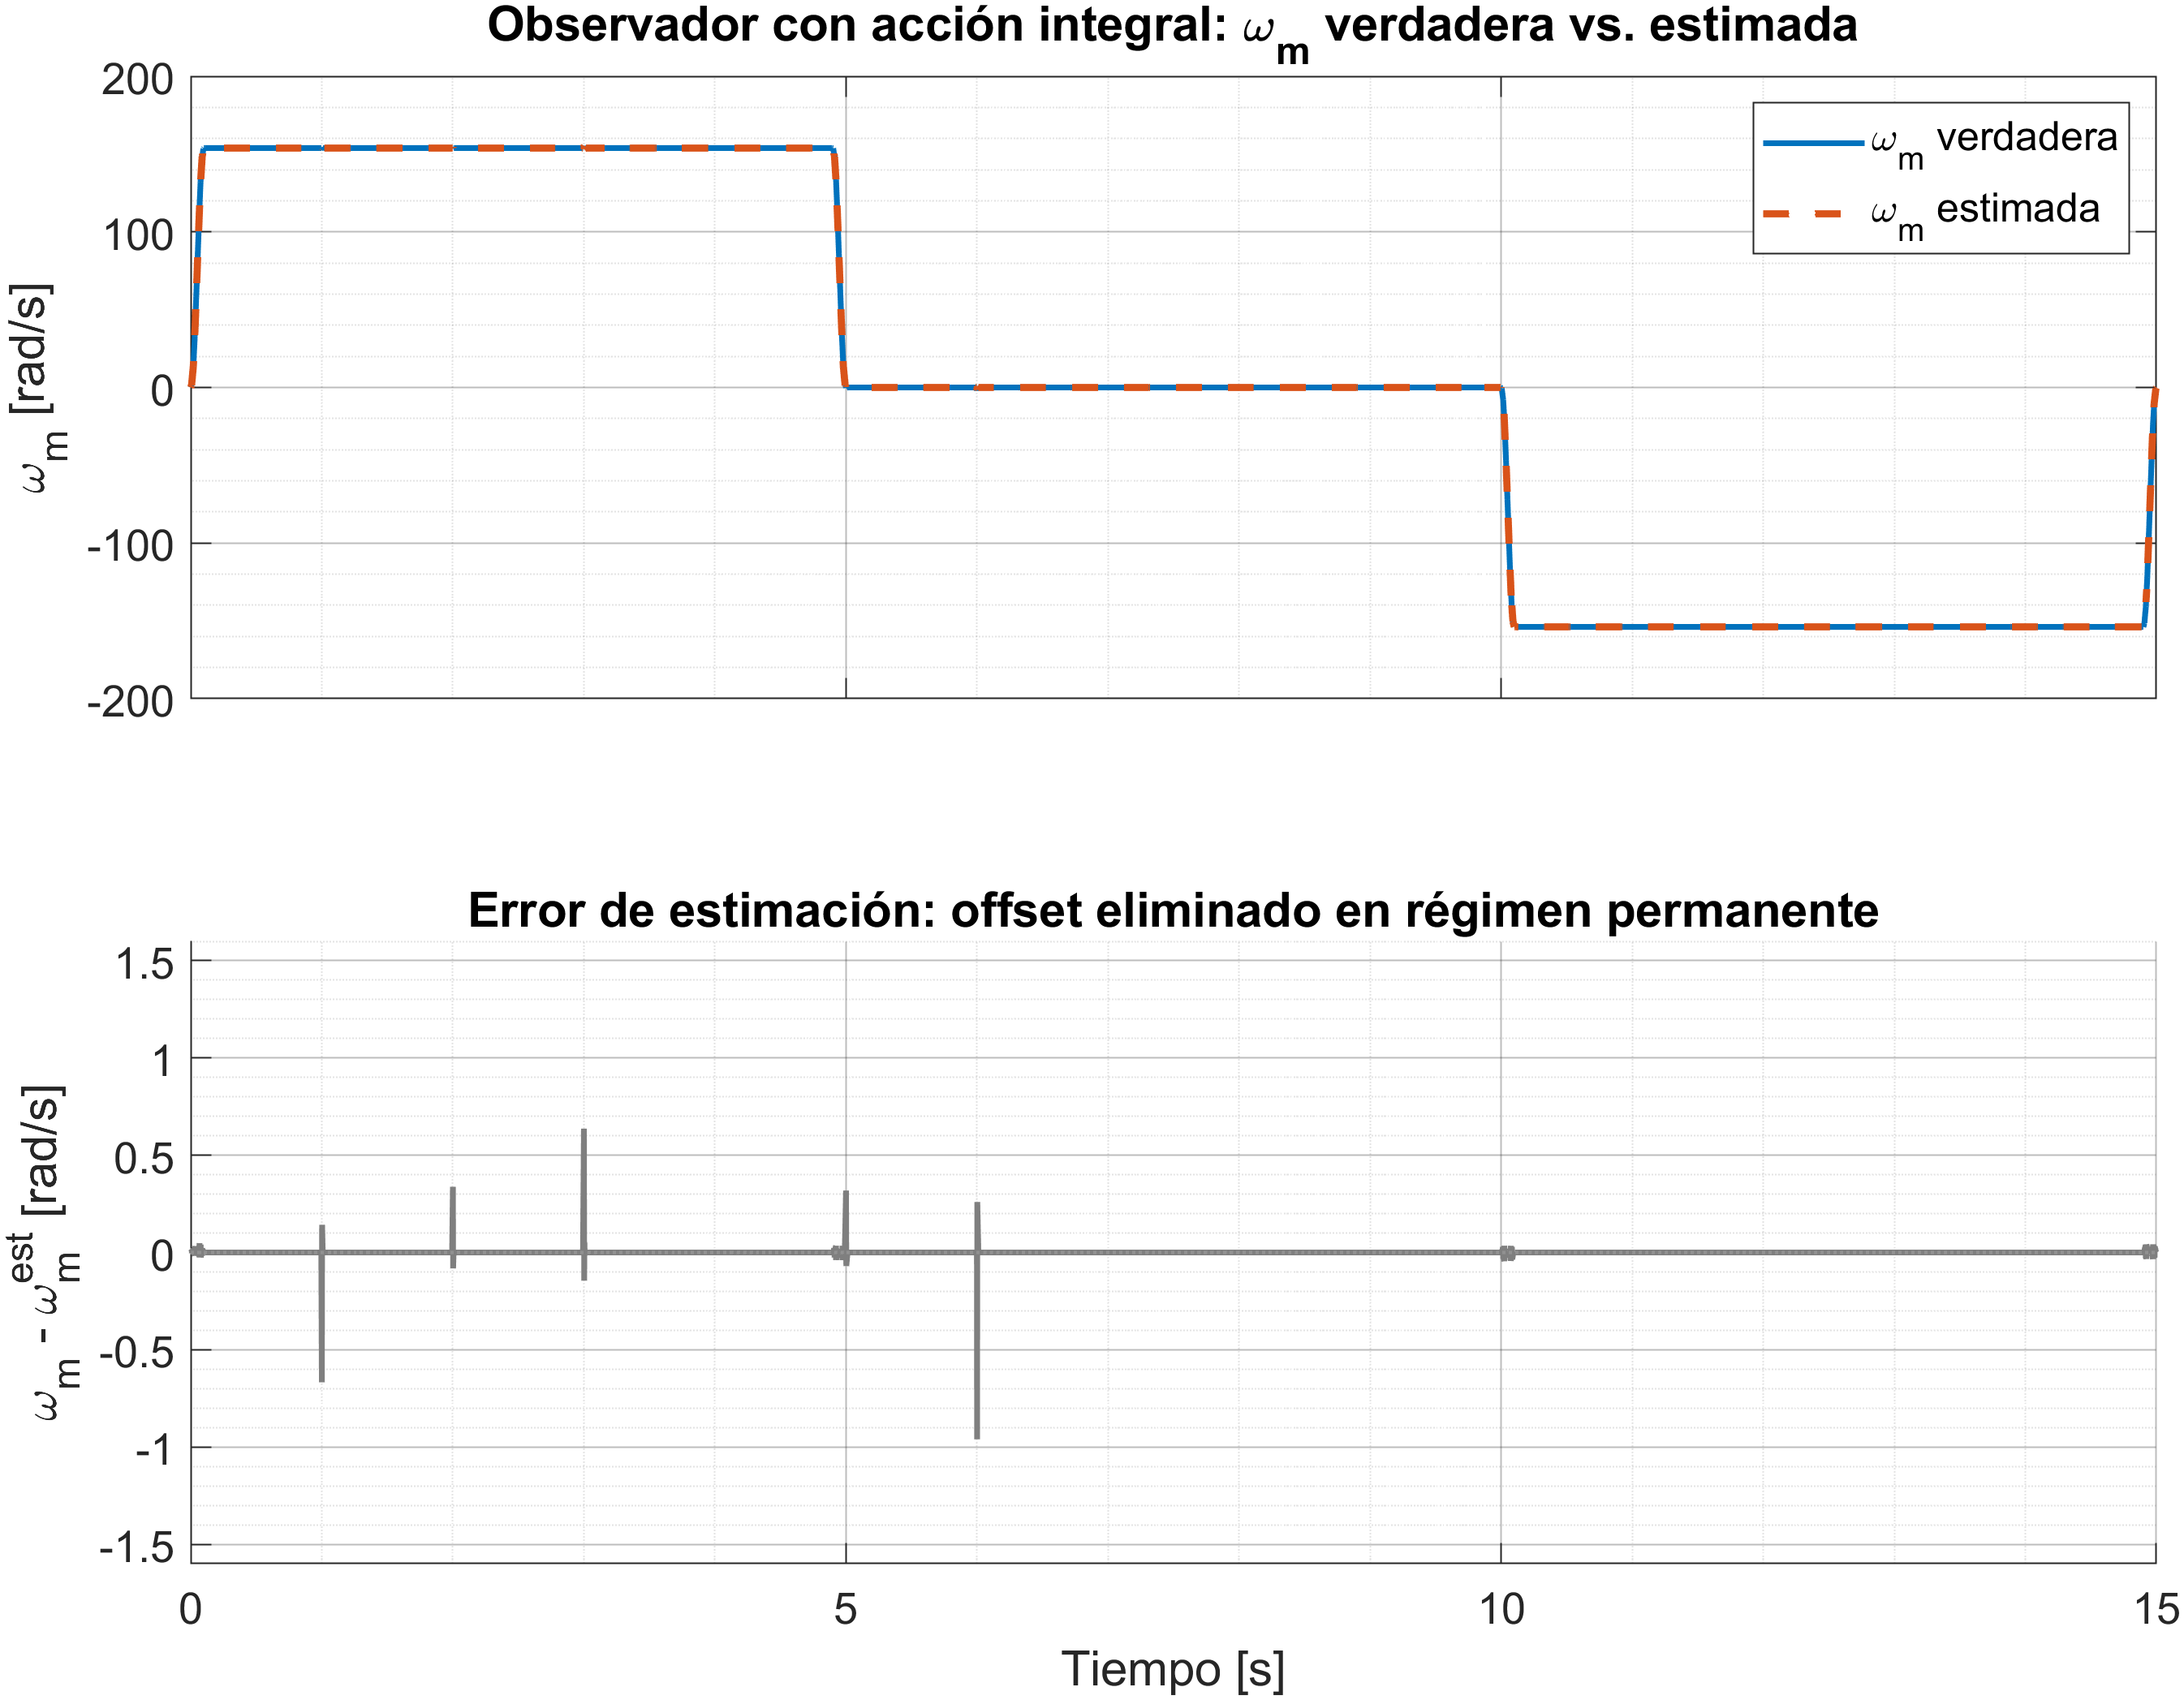
\includegraphics[width=0.78\linewidth]{imagenes/5_2_5_B_observador_sin_offset.png}
    \caption{Respuesta del observador aumentado con acción integral. Se observa la desaparición del error de offset en régimen permanente.}
    \label{fig:obs_offset_corregido}
\end{figure}

Comparando las Fig.~\ref{fig:obs_offset_original} y \ref{fig:obs_offset_corregido}, se verifica que el agregado del estado integral corrige el error de estimación de régimen permanente sin perder una rapidez de convergencia compatible con el resto de la arquitectura de control. Por este motivo, el observador mecánico aumentado con acción integral se adopta como solución final.

\subsection{Comportamiento térmico del motor}

Para verificar el comportamiento térmico del accionamiento en operación repetitiva, se aplicó de manera cíclica la consigna final de posición adoptada en el trabajo, compuesta por un trapecio de 15 s de duración: rampa de subida entre 0 y 5 s, mantenimiento entre 5 y 10 s, y rampa de bajada entre 10 y 15 s. Sobre esta condición de funcionamiento se consideró una temperatura ambiente de
\[
T_{amb}^\circ=25^\circ\text{C}
\]
y un torque de perturbación máximo de
\[
T_{ld}=5\ \text{Nm}.
\]

La simulación se ejecutó repitiendo sucesivamente dicho ciclo, de modo de evaluar la evolución de la temperatura del bobinado del estator \(T_s^\circ(t)\). Dado que cada ciclo tiene una duración de 15 s, el instante en que se supera la temperatura máxima admisible
\[
T^\circ_{s,max}=115^\circ\text{C}
\]
ocurre a los
\[
t=225{,}9\ \text{s},
\]
lo que corresponde a aproximadamente 15 ciclos completos y 0{,}9 s del ciclo número 16.

\begin{figure}[H]
    \centering
    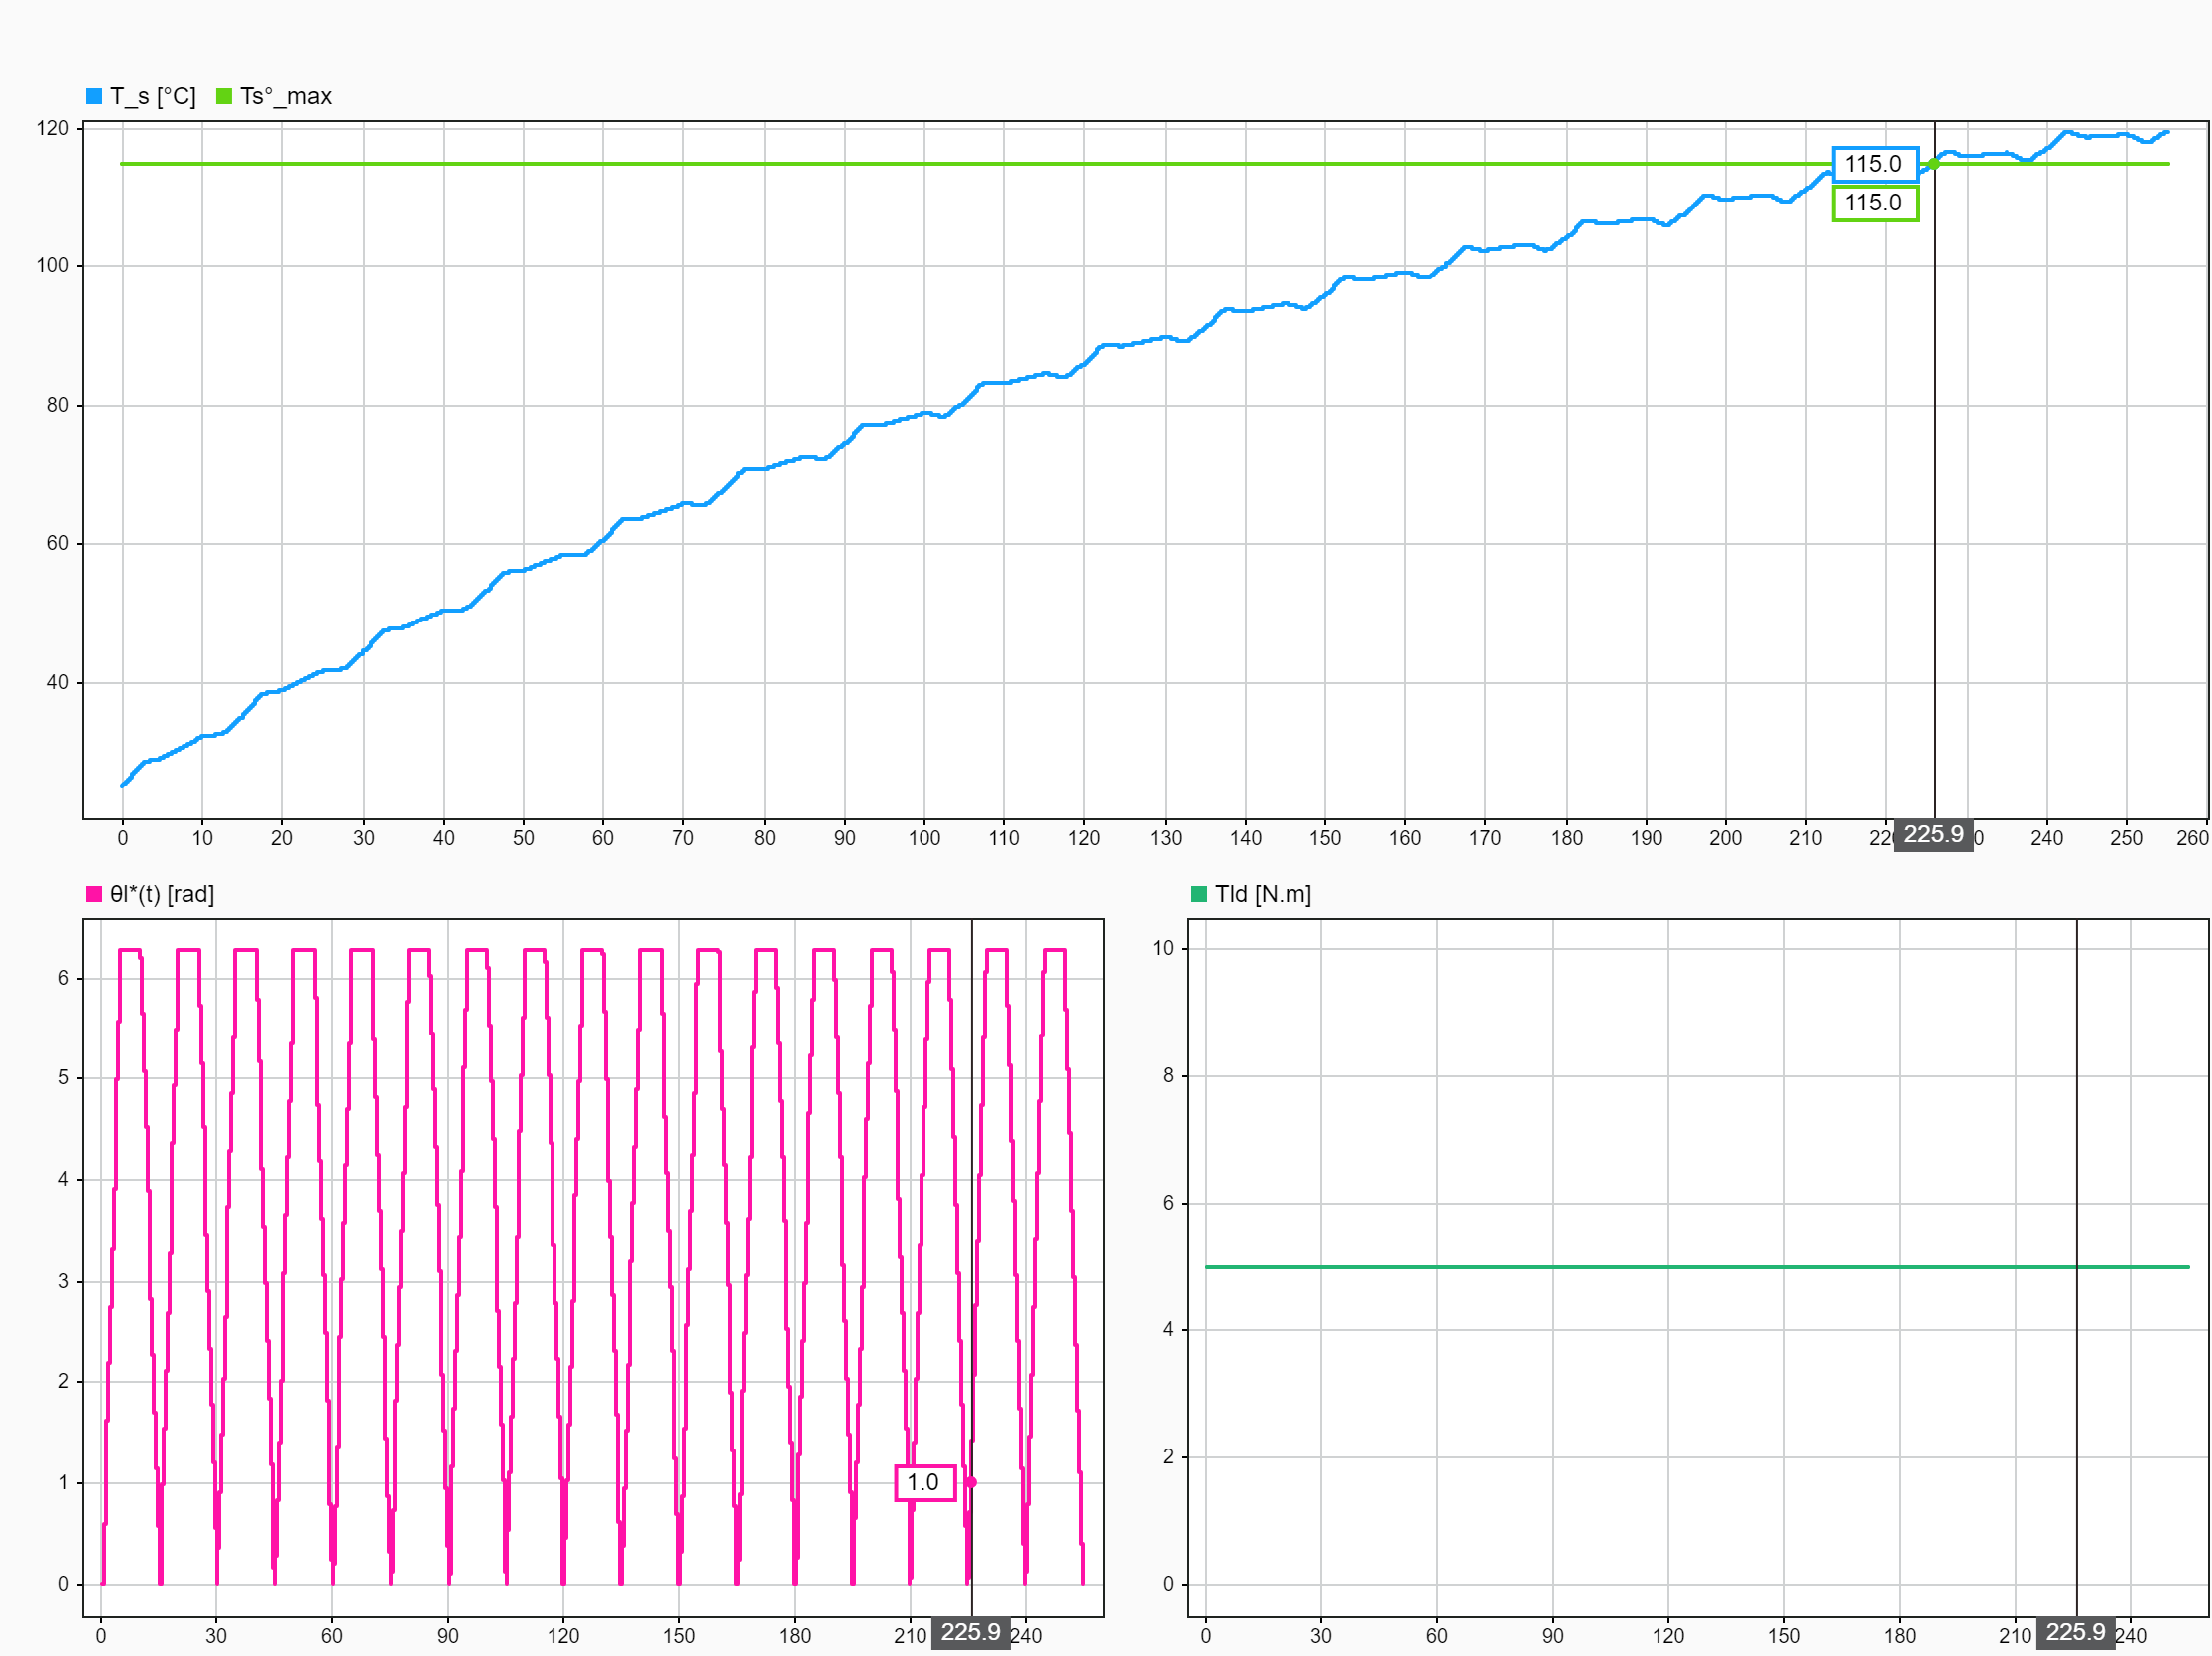
\includegraphics[width=0.9\linewidth]{imagenes/5_2_5_C_comportamiento_termico.png}
    \caption{Evolución de la temperatura del bobinado \(T_s^\circ(t)\) bajo operación repetitiva, considerando \(T_{amb}^\circ=25^\circ\text{C}\), \(T_{ld}=5\,\text{Nm}\) y la consigna trapezoidal de posición utilizada en el trabajo. Se observa que la temperatura supera el límite admisible \(T^\circ_{s,max}=115^\circ\text{C}\) a los 225{,}9 s.}
    \label{fig:termico_525c}
\end{figure}

Por lo tanto, para las condiciones analizadas, el sistema no satisface el requerimiento térmico de operación continua repetitiva, ya que la temperatura del bobinado excede el valor máximo permitido antes de alcanzar el equilibrio térmico. En consecuencia, esta condición de trabajo no resulta admisible desde el punto de vista térmico.
%-------------
\subsubsection{Evaluación de desempeño utilizando sensores no ideales ($G(s)\neq 1$)}
En esta sección se evalúa el desempeño del sistema asumiendo una función de transferencia para los sensores, de modo que se comporten como filtros pasa bajos. Para ello, la consigna detalla un punto de partida para los polos de las funciones de transferencia a aplicar mediante el modelo en espacio de estados (SS).

Se reemplaza entonces el modelo ideal de medición $G(s)=1$ por modelos dinámicos equivalentes de filtros pasa bajos con ganancia unitaria, implementados en espacio de estados. Los sensores afectados son las corrientes de fase, la posición angular del rotor y la medición de temperatura del estator, con los parámetros indicados en la consigna~\cite{guia_trabajo}.

\subsubsection*{Polos requeridos para cada sensor}

Tomando como referencia la forma estándar de un filtro pasa bajos de primer y segundo orden, los polos requeridos para cada sensor son los que se resumen en la Tabla~\ref{tab:polos_sensores}.

\begin{table}[H]
    \centering
    \caption{Polos requeridos para los modelos de sensores no ideales}
    \label{tab:polos_sensores}
    \begin{tabular}{|c|c|c|c|}
        \hline
        \textbf{Sensor} & \textbf{Modelo} & \textbf{Parámetros} & \textbf{Polos} \\
        \hline
        $i_{as}(t),\,i_{bs}(t),\,i_{cs}(t)$ 
        & LP 2$^\circ$ orden 
        & $\omega_n=6000\ \text{rad/s},\ \zeta=1$ 
        & $p_{1,2}=-6000$ \\
        \hline
        $\theta_m(t)$ 
        & LP 2$^\circ$ orden 
        & $\omega_n=2000\ \text{rad/s},\ \zeta=1$ 
        & $p_{1,2}=-2000$ \\
        \hline
        $T_s^\circ(t)$ 
        & LP 1$^\circ$ orden 
        & $\tau=20\ \text{s}$ 
        & $p=-\dfrac{1}{\tau}=-0{,}05$ \\
        \hline
    \end{tabular}
\end{table}

Para los filtros de segundo orden se parte de la función de transferencia estándar con ganancia estática unitaria:
\begin{equation}
    G_{LP,2}(s)=\frac{\omega_n^2}{s^2+2\zeta\omega_n s+\omega_n^2}.
    \label{eq:lp2_tf}
\end{equation}

Los polos asociados resultan de resolver la ecuación característica
\begin{equation}
    s^2+2\zeta\omega_n s+\omega_n^2=0,
\end{equation}
por lo que
\begin{equation}
    p_{1,2}=-\zeta\omega_n\pm\omega_n\sqrt{\zeta^2-1}.
\end{equation}

Como en este caso se adopta $\zeta=1$, ambos filtros de segundo orden quedan críticamente amortiguados, con polo doble en
\begin{equation}
    p_1=p_2=-\omega_n.
\end{equation}

Por otra parte, para el sensor térmico se emplea un filtro pasa bajos de primer orden con ganancia unitaria:
\begin{equation}
    G_{LP,1}(s)=\frac{1}{\tau s+1},
    \label{eq:lp1_tf}
\end{equation}
cuyo polo se ubica en
\begin{equation}
    p=-\frac{1}{\tau}.
\end{equation}

\subsubsection*{Obtención del modelo en espacio de estados}

A continuación se desarrolla la obtención de las matrices $A$, $B$ y $C$ para cada tipo de filtro, partiendo de sus funciones de transferencia estándar.

\subsubsection*{Filtro pasa bajos de primer orden}

Partiendo de \eqref{eq:lp1_tf}:

\begin{equation}
    \frac{Y(s)}{U(s)}=\frac{1}{\tau s+1}.
\end{equation}
\begin{equation}
    (\tau s+1)Y(s)=U(s).
\end{equation}

Aplicando transformada inversa de Laplace:
\begin{equation}
    \tau \dot{y}(t)+y(t)=u(t).
\end{equation}

Despejando la derivada:
\begin{equation}
    \dot{y}(t)=-\frac{1}{\tau}y(t)+\frac{1}{\tau}u(t).
\end{equation}

Si se elige como variable de estado
\begin{equation}
    x(t)=y(t),
\end{equation}
entonces el modelo en espacio de estados queda:
\begin{equation}
    \dot{x}(t)=Ax(t)+Bu(t), \qquad y(t)=Cx(t),
\end{equation}
con
\begin{equation}
    A=\begin{bmatrix}
        -\dfrac{1}{\tau}
    \end{bmatrix},
    \qquad
    B=\begin{bmatrix}
        \dfrac{1}{\tau}
    \end{bmatrix},
    \qquad
    C=\begin{bmatrix}
        1
    \end{bmatrix}.
\end{equation}

Por lo tanto, para el sensor de temperatura con $\tau=20\ \text{s}$:
\begin{equation}
    A_T=\begin{bmatrix}
        -0{,}05
    \end{bmatrix},
    \qquad
    B_T=\begin{bmatrix}
        0{,}05
    \end{bmatrix},
    \qquad
    C_T=\begin{bmatrix}
        1
    \end{bmatrix}.
\end{equation}

\subsubsection*{Filtro pasa bajos de segundo orden}

Partiendo de \eqref{eq:lp2_tf}:
\begin{equation}
    \frac{Y(s)}{U(s)}=\frac{\omega_n^2}{s^2+2\zeta\omega_n s+\omega_n^2}.
\end{equation}
\begin{equation}
    (s^2+2\zeta\omega_n s+\omega_n^2)Y(s)=\omega_n^2 U(s).
\end{equation}

Aplicando transformada inversa de Laplace:
\begin{equation}
    \ddot{y}(t)+2\zeta\omega_n \dot{y}(t)+\omega_n^2 y(t)=\omega_n^2 u(t).
\end{equation}

Ahora se define el vector de estado como
\begin{equation}
    x_1(t)=y(t), \qquad x_2(t)=\dot{y}(t).
\end{equation}

Entonces:
\begin{equation}
    \dot{x}_1(t)=x_2(t),
\end{equation}
\begin{equation}
    \dot{x}_2(t)= -\omega_n^2 x_1(t)-2\zeta\omega_n x_2(t)+\omega_n^2 u(t).
\end{equation}

En forma matricial:
\begin{equation}
    \dot{x}(t)=Ax(t)+Bu(t), \qquad y(t)=Cx(t),
\end{equation}
con
\begin{equation}
    A=
    \begin{bmatrix}
        0 & 1 \\
        -\omega_n^2 & -2\zeta\omega_n
    \end{bmatrix},
    \qquad
    B=
    \begin{bmatrix}
        0 \\
        \omega_n^2
    \end{bmatrix},
    \qquad
    C=
    \begin{bmatrix}
        1 & 0
    \end{bmatrix}.
\end{equation}

\subsubsection*{Aplicación al sensor de corriente}

Para los sensores de corriente se adopta $\omega_n=6000\ \text{rad/s}$ y $\zeta=1$, luego:
\begin{equation}
    A_i=
    \begin{bmatrix}
        0 & 1 \\
        -6000^2 & -2\cdot 1 \cdot 6000
    \end{bmatrix}
    =
    \begin{bmatrix}
        0 & 1 \\
        -3{,}6\times 10^7 & -1{,}2\times 10^4
    \end{bmatrix},
\end{equation}
\begin{equation}
    B_i=
    \begin{bmatrix}
        0 \\
        6000^2
    \end{bmatrix}
    =
    \begin{bmatrix}
        0 \\
        3{,}6\times 10^7
    \end{bmatrix},
    \qquad
    C_i=
    \begin{bmatrix}
        1 & 0
    \end{bmatrix}.
\end{equation}

Este mismo modelo se aplica de manera idéntica a $i_{as}(t)$, $i_{bs}(t)$ e $i_{cs}(t)$.

\subsubsection*{Aplicación al sensor de posición}

Para el sensor de posición angular se adopta $\omega_n=2000\ \text{rad/s}$ y $\zeta=1$, por lo que:
\begin{equation}
    A_\theta=
    \begin{bmatrix}
        0 & 1 \\
        -2000^2 & -2\cdot 1 \cdot 2000
    \end{bmatrix}
    =
    \begin{bmatrix}
        0 & 1 \\
        -4{,}0\times 10^6 & -4{,}0\times 10^3
    \end{bmatrix},
\end{equation}
\begin{equation}
    B_\theta=
    \begin{bmatrix}
        0 \\
        2000^2
    \end{bmatrix}
    =
    \begin{bmatrix}
        0 \\
        4{,}0\times 10^6
    \end{bmatrix},
    \qquad
    C_\theta=
    \begin{bmatrix}
        1 & 0
    \end{bmatrix}.
\end{equation}

\subsubsection*{Resumen de modelos en espacio de estados}

Finalmente, los modelos de sensores no ideales a implementar quedan definidos como:

\begin{equation}
    \dot{x}_i(t)=A_i x_i(t) + B_i u_i(t), \qquad y_i(t)=C_i x_i(t),
\end{equation}
para los sensores de corriente,

\begin{equation}
    \dot{x}_\theta(t)=A_\theta x_\theta(t) + B_\theta u_\theta(t), \qquad y_\theta(t)=C_\theta x_\theta(t),
\end{equation}
para el sensor de posición angular, y

\begin{equation}
    \dot{x}_T(t)=A_T x_T(t) + B_T u_T(t), \qquad y_T(t)=C_T x_T(t),
\end{equation}
para el sensor de temperatura.

En todos los casos, la entrada $u(t)$ corresponde a la variable física real a medir, mientras que la salida $y(t)$ representa la señal efectivamente medida por el sensor no ideal. Para evitar transitorios artificiales al inicio de la simulación, las condiciones iniciales de cada filtro deben fijarse de forma consistente con el valor inicial de la magnitud medida.

\subsubsection*{Simulación con sensores no ideales}
\begin{figure}[H]
    \centering
    
\includegraphics[width=0.8\textwidth]{imagenes/sensores_no_ideales_1.png}
    \caption{\textit{Arriba: posición y velocidad; abajo: corriente en eje de cuadratura.} Puede verse el efecto del modelo en SS de los sensores, con el cual el sistema no puede seguir la consigna de posición. ($T_{ld} = 5 \ [Nm]$)}
    \label{fig:sens_pos_1}
\end{figure}
Es interesante observar en la Fig.~\ref{fig:sens_pos_1} cómo, con los polos elegidos para el modelo, los sensores no son lo suficientemente rápidos respecto a la dinámica del lazo de corriente, lo que era de esperarse: si se recuerda el diseño del modulador de corriente, se habían elegido $p_i=-5000 \ [rad/s]$, por lo que modelar los sensores de corriente con $p_{sens,abc}=-6000 \ [rad/s]$ no resulta lo suficientemente más rápido que la dinámica del sistema. Lo mismo ocurre con los polos del observador. Por eso se propone aumentar estos polos de forma conjunta, es decir, $\omega_n^{\prime} = N \cdot \omega_n;\ N=1,2,3\ldots$
Luego de experimentar, se obtienen resultados aceptables con $N=3$ (Fig. \ref{fig:sens_pos_2}). Esto indicaría que los sensores a utilizar en el accionamiento deberían presentar una respuesta por lo menos tres veces más rápida que los del modelo especificado inicialmente en la consigna.
 \begin{figure}[H]
    \centering
    
\includegraphics[width=0.8\textwidth]{imagenes/sensores_no_ideales_2.png}
    \caption{\textit{Arriba: posición y velocidad; abajo: corriente en eje de cuadratura.} Puede verse que el accionamiento ya sigue con éxito la consigna solicitada, sin oscilaciones producidas por los retardos de los sensores. ($T_{ld} = 5 \ [Nm]$)}
    \label{fig:sens_pos_2}
\end{figure}
\subsubsection*{Análisis de respuesta simulando no idealidad de inversor trifásico de tensión}
En un accionamiento físico real, el inversor está restringido por las limitaciones dinámicas de los dispositivos semiconductores de conmutación (como los transistores MOSFETs o IGBTs) y por el nivel máximo de energía que puede proveer su fuente de alimentación de corriente continua.
Para evaluar de manera fidedigna cómo estas limitaciones degradan el desempeño del sistema, se reemplaza el bloque ideal por un modelo equivalente estructurado en espacio de estados (SS) que incorpora dos restricciones físicas fundamentales: un ancho de banda limitado y la saturación estricta de la tensión.
Se propone, a priori, simular esta limitación como un filtro pasa bajo de segundo orden con amortiguación crítica ($\zeta = 1$) y $\omega_n = 6000 \ [rad/s]$, con lo que, siguiendo el desarrollo del punto anterior, las matrices $A_v$ y $B_v$ del espacio de estados quedarían:
\begin{equation*}
    A_v=
    \begin{bmatrix}
        0 & 1 \\
        -\omega_n^2 & -2\zeta\omega_n
    \end{bmatrix},
    \qquad
    B_v=
    \begin{bmatrix}
        0 \\
        \omega_n^2
    \end{bmatrix},
    \qquad
    C_v=
    \begin{bmatrix}
        1 & 0
    \end{bmatrix}.
\end{equation*}
 \begin{figure}[H]
    \centering
    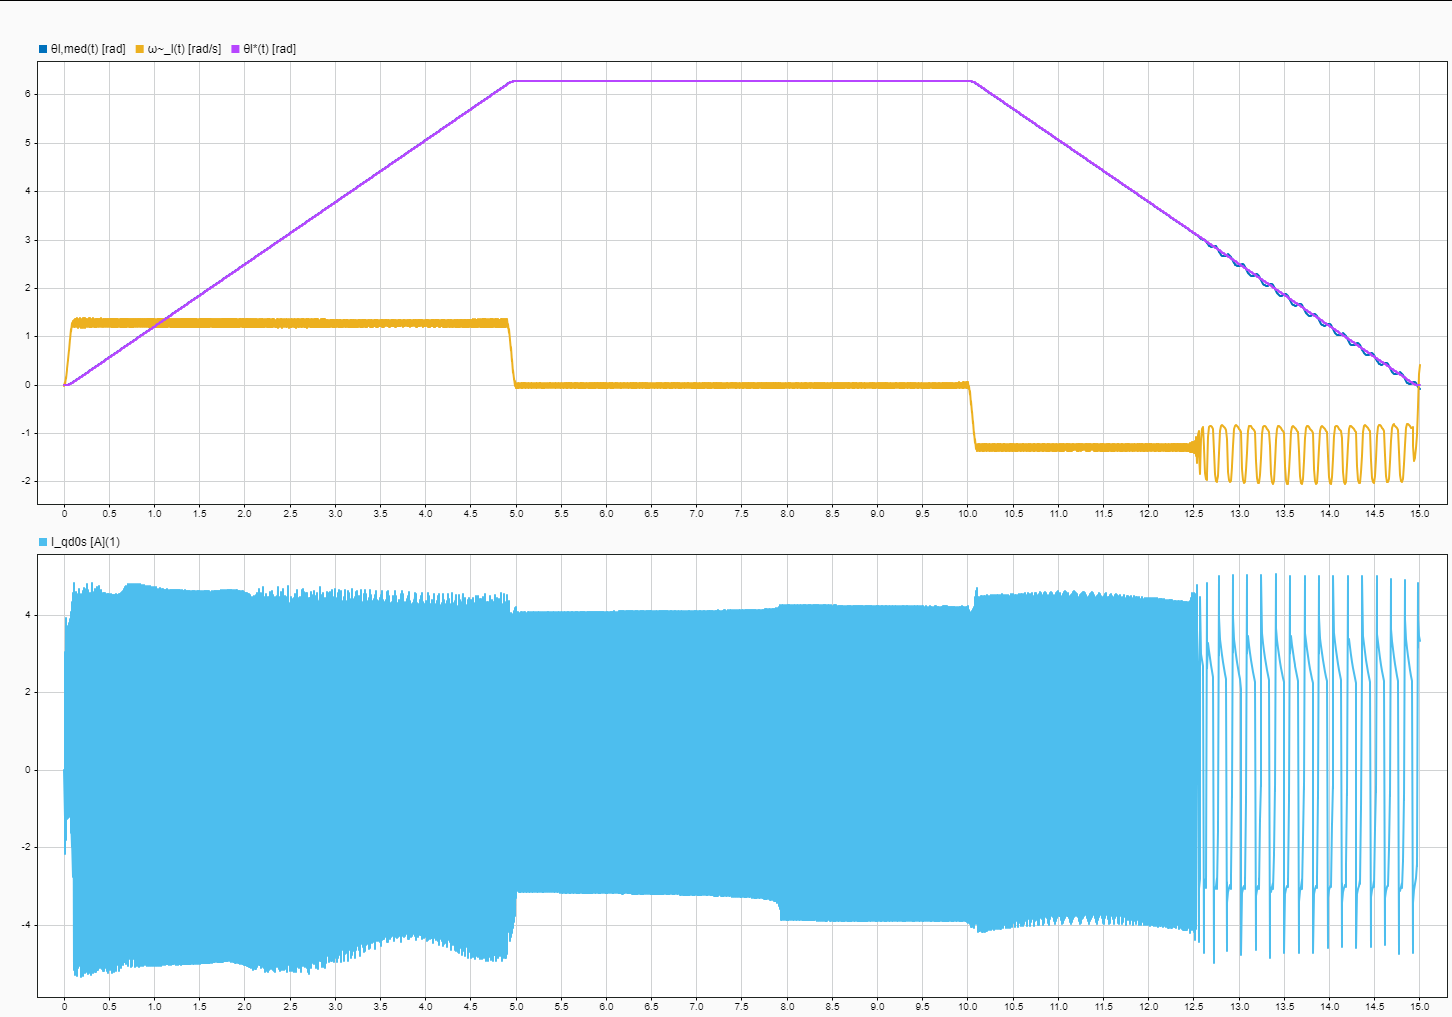
\includegraphics[width=0.8\textwidth]{imagenes/inversor_no_ideal_6000.png}
    \caption{\textit{Arriba: posición y velocidad; abajo: corriente en eje de cuadratura.} Puede verse que el inversor no es lo suficientemente rápido. ($T_{ld} = 5 \ [Nm]$, $\omega_n = 6000 \ [rad/s]$)}
    \label{fig:inv_trifasico_6000}
\end{figure}
Como era de esperarse, la rapidez propuesta inicialmente no es suficiente, ya que es solo un $20\%$ más rápida que el lazo de corriente. Se propone, siguiendo el mismo procedimiento que en el modelado de los sensores, duplicar la rapidez de respuesta del inversor a $\omega_n^{\prime} = 12000 \ [rad/s]$.
 \begin{figure}[H]
    \centering
    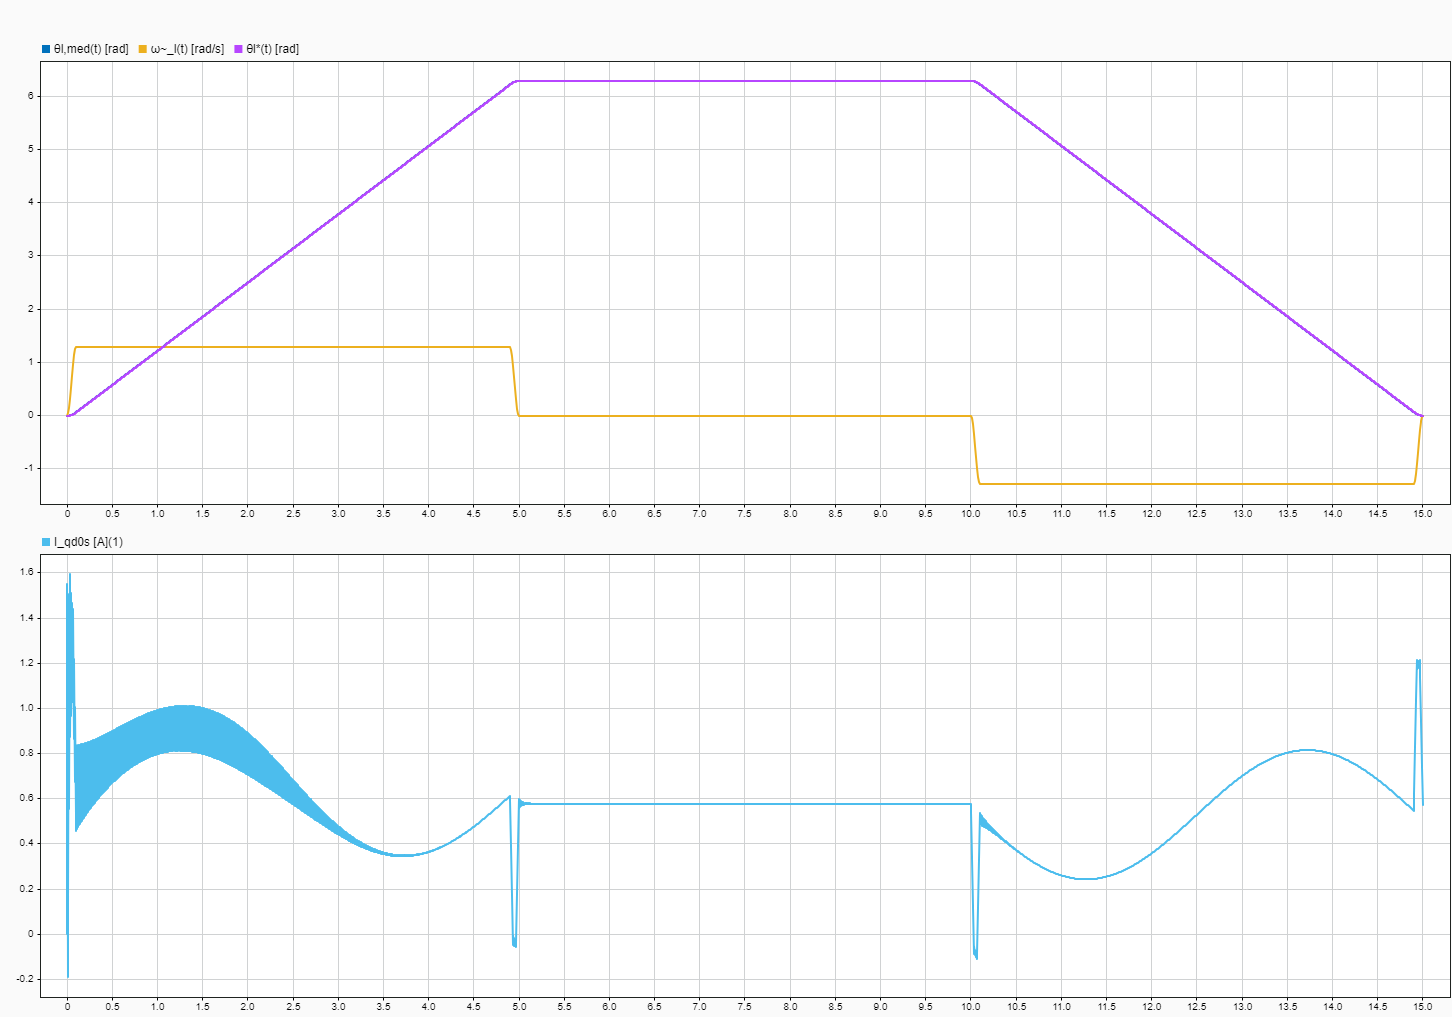
\includegraphics[width=0.8\textwidth]{imagenes/inversor_no_ideal_12000.png}
    \caption{\textit{Arriba: posición y velocidad; abajo: corriente en eje de cuadratura.} Finalmente se consigue un desempeño satisfactorio y, al mismo tiempo, el cumplimiento de las demás condiciones de operación. ($T_{ld} = 5 \ [Nm]$, $\omega_n = 12000 \ [rad/s]$)}
    \label{fig:inv_trifasico_12000}
\end{figure}
\section{Discretización del Controlador}

Para posibilitar la implementación física del algoritmo de control en un microcontrolador industrial o procesador digital de señales (DSP), es necesario efectuar la transición del diseño desde el tiempo continuo (dominio de Laplace, $s$) al tiempo discreto (dominio $z$). En el entorno digital, el controlador no evalúa las señales de forma ininterrumpida, sino que adquiere muestras y computa ecuaciones en diferencias algebraicas a intervalos regulares de tiempo.

El primer paso crítico en este diseño es la determinación del período de muestreo $T_s$ (que no debe confundirse con la temperatura del estator $T_s^\circ$, la cual lleva siempre el superíndice de grado). Según el criterio práctico de diseño de sistemas de control digital, la frecuencia de muestreo $f_s = 1/T_s$ debe ser al menos 10 veces mayor que el ancho de banda del lazo de control más rápido, garantizando así que no se degrade la estabilidad global del sistema. En la arquitectura desarrollada, el lazo proporcional de corrientes posee la dinámica más veloz con un ancho de banda $BW_{cont} = 796 \ \mathrm{Hz}$. Por consiguiente, el período de muestreo nominal exigido se calcula como:
\begin{equation}
    T_s \leq \frac{1}{10 \cdot 796} \approx 1{,}25 \times 10^{-4} \ \mathrm{s}.
\end{equation}

\subsection{Método de integración de Tustin}
Para llevar a cabo la discretización de los elementos con inercia dinámica, específicamente los bloques integradores ($1/s$), se emplea el método de Tustin, también conocido como aproximación bilineal o regla de integración trapezoidal. Este método destaca por su robustez analítica frente a otros métodos numéricos, dado que mapea todo el semiplano izquierdo del plano complejo $s$ estrictamente dentro del círculo unitario en el plano $z$, lo que asegura que si el sistema en tiempo continuo es estable, su equivalente discreto también lo será.

Físicamente, el método aproxima la integral temporal de una señal calculando el área bajo la curva mediante el trazado de trapecios (líneas rectas) entre dos instantes de muestreo consecutivos. Matemáticamente, la transformación bilineal de Tustin se define sustituyendo el operador continuo de Laplace $s$ por su equivalente discreto dependiente del período de muestreo:
\begin{equation}
    s \approx \frac{2}{T_s} \frac{1 - z^{-1}}{1 + z^{-1}}
\end{equation}

Al aplicar esta sustitución a la función de transferencia de un integrador puro ($H(s) = 1/s$), se obtiene la función de transferencia en el dominio $z$:
\begin{equation}
    H(z) = \frac{Y(z)}{X(z)} = \frac{T_s}{2} \left( \frac{1 + z^{-1}}{1 - z^{-1}} \right)
\end{equation}

Aplicando la transformada $Z$ inversa a esta expresión, se obtiene la ley de actualización (o ecuación en diferencias recursiva) que el microprocesador debe ejecutar secuencialmente en cada paso de cálculo $k$:
\begin{equation}
    y[k] = y[k-1] + \frac{T_s}{2} \big( x[k] + x[k-1] \big)
\end{equation}
donde $x[k]$ y $x[k-1]$ representan la entrada muestreada actual y pasada al integrador, mientras que $y[k]$ y $y[k-1]$ representan la salida (área acumulada) actual y pasada, respectivamente.

\subsubsection{Implementación en la arquitectura de control}
En el diagrama general del sistema, el algoritmo de Tustin detallado se aplica exclusivamente para sustituir los bloques con memoria, es decir, la acción integral del controlador PID de movimiento ($K_{sia}/s$) y los múltiples integradores internos del observador de estado de orden reducido.

Por otro lado, los bloques netamente algebraicos como el modulador de torque y el modulador de corriente carecen de dinámica integradora, por lo que su discretización consiste en operar sus ecuaciones trigonométricas y proporcionales sincronizadas bajo el mismo reloj base $T_s$. Finalmente, la frontera entre el controlador digital y el mundo físico continuo (el motor y los actuadores) se modela empleando retenedores de orden cero (ZOH), los cuales emulan a los conversores digital-analógicos manteniendo retenida la señal de control en forma de escalón durante todo el ciclo $T_s$.
\begin{figure}[H]
    \centering
    
\includegraphics[width=0.8\textwidth]{imagenes/observador_discretizado.png}
    \caption{Diagrama de bloques del observador discretizado. Incorporación de ZOH y reemplazo de integradores continuos por integradores de Tustin.}
\end{figure}
\begin{figure}[H]
    \centering
    
\includegraphics[width=0.8\textwidth]{imagenes/controladorPID_discretizado.png}
    \caption{Diagrama de bloques del controlador de posición discretizado. Incorporación de ZOH y reemplazo de integradores continuos por integradores de Tustin.}
\end{figure}
\section{Codificación del Software de Control}

La implementación del controlador se organizó de forma modular, separando cada etapa del lazo de control en una \textit{MATLAB Function} independiente. Esta estructura permite reproducir en código el mismo flujo de señales desarrollado previamente en Simulink, manteniendo una correspondencia directa entre los bloques del diagrama y las funciones programadas. De esta manera, cada función recibe únicamente las variables necesarias para su cálculo, procesa la información correspondiente y entrega sus salidas hacia la siguiente etapa del controlador.

El flujo general de información comienza con el generador de trayectoria, encargado de entregar las referencias cinemáticas del movimiento: posición, velocidad y aceleración. Estas señales definen la evolución deseada del eje del motor y evitan aplicar consignas abruptas directamente sobre el sistema. La referencia de velocidad se compara luego con la velocidad estimada del motor, generando el error utilizado por el controlador de posición.

Como la velocidad mecánica no se mide directamente, se emplea un observador de estado reducido. Este bloque recibe la posición medida $\theta_m$ y el torque electromagnético de referencia $T_m^{*}$, y a partir de esas señales estima la velocidad mecánica $\hat{\omega}_m$. Esta velocidad estimada se realimenta hacia el controlador de posición y hacia el modulador de torque, cerrando el lazo externo de movimiento.

El controlador PID de posición calcula una referencia de torque mecánico $T_m^{**}$ a partir del error de velocidad. Internamente conserva los estados de sus integradores mediante variables \texttt{persistent}, lo que permite ejecutar la ecuación recursiva en cada instante de muestreo sin perder la memoria del ciclo anterior. La salida de este bloque representa el esfuerzo mecánico requerido para que el eje siga la trayectoria impuesta.

A continuación, el modulador de torque convierte la referencia $T_m^{**}$ en una referencia de corriente de eje $q$, $i_{qs}^{r*}$. Para ello incorpora compensaciones de fricción viscosa y de torque gravitatorio, además de la constante de torque propia de la PMSM. De esta forma, el lazo externo no entrega directamente una tensión al motor, sino una corriente de referencia asociada al torque electromagnético requerido.

El modulador de corriente constituye el lazo interno del controlador. Este bloque compara las corrientes de referencia $i_{qs}^{r*}$, $i_{ds}^{r*}$ e $i_{0s}^{*}$ con las corrientes medidas en coordenadas $qd0$, generando las tensiones de control $v_{qs}^{r*}$, $v_{ds}^{r*}$ y $v_{0s}^{*}$. Estas tensiones son todavía señales de control ideales, por lo que luego se corrigen mediante el bloque de desacople.

El desacople de realimentaciones físicas naturales agrega a las tensiones de control los términos eléctricos propios de la máquina, como las caídas resistivas y las fuerzas contraelectromotrices dependientes de la velocidad. Con esto se obtienen las tensiones finales $v_{qs}^r$, $v_{ds}^r$ y $v_{0s}$ que deben aplicarse en el marco rotórico.

Finalmente, la transformación inversa de Park convierte las tensiones en coordenadas $qd0$ hacia el sistema trifásico $abc$, generando las consignas $v_{as}^*$, $v_{bs}^*$ y $v_{cs}^*$ para el inversor. En sentido opuesto, la transformación directa de Park toma las corrientes trifásicas medidas y las expresa como $i_{qs}^r$, $i_{ds}^r$ e $i_{0s}$, permitiendo que los lazos de corriente trabajen sobre variables desacopladas y físicamente interpretables.

En conjunto, las \textit{MATLAB Functions} se comunican mediante señales escalares y una estructura común de parámetros, denominada \texttt{params}. Las señales escalares representan las variables instantáneas del sistema, mientras que \texttt{params} concentra las constantes del motor, del reductor, de la carga mecánica y de los controladores. Esta organización simplifica la lectura del código, evita repetir parámetros en distintos bloques y facilita futuras modificaciones de sintonía sin alterar la lógica principal de cada función.
\subsection{Código de cada parte del controlador}


\subsubsection{Controlador PID de posición}
El controlador PID de posición constituye el lazo externo del sistema de control. Su entrada es el error de velocidad $e_\omega$, obtenido a partir de la referencia de movimiento y la velocidad estimada por el observador. A partir de este error, el bloque calcula la referencia de torque mecánico $T_m^{**}$ que debe desarrollar el accionamiento. La implementación discreta utiliza integradores de Tustin, cuyos estados anteriores se almacenan mediante variables \texttt{persistent}.
\begin{figure}[H]
    \centering
    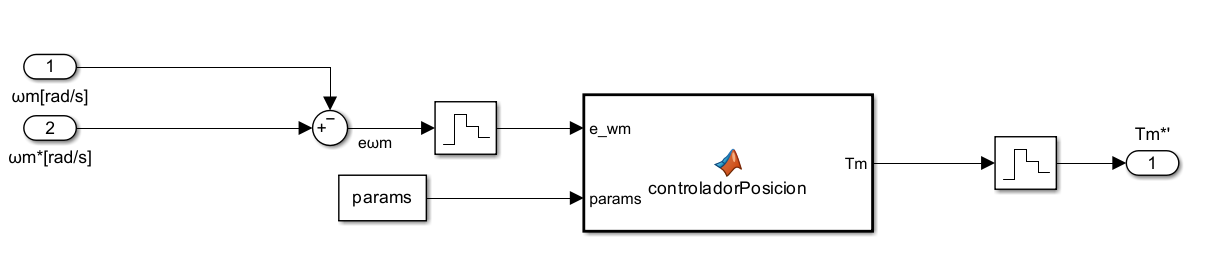
\includegraphics[width=0.60\linewidth]{imagenes/codificado_PIDpos.png}
    \caption{Código implementado para el controlador PID de posición.}
    \label{fig:codificado_PIDpos}
\end{figure}
\begin{lstlisting}[
caption={Código MATLAB Function del controlador de posición discretizado.},
label={lst:controlador_posicion}
]
function Tm = controladorPosicion(e_wm,params)
% Calcula la orden de torque Tm** en función del error de velocidad e_wm[k]
% usando integradores discretos tipo Tustin.
%
%   Ts   – periodo de muestreo
%   b_a  – ganancia del término proporcional (error de velocidad)
%   K_sa – ganancia del primer integrador (error de posición)
%   K_sia– ganancia del segundo integrador

    Ts   = params.Ts;
    b_a  = params.b_a;
    K_sa = params.K_sa;
    K_sia= params.K_sia;
    % Variables persistentes para almacenar estados entre llamadas
    persistent e_theta_prev e_theta_int_prev e_prev
    if isempty(e_theta_prev)
        e_theta_prev    = 0;   % integral del error de velocidad en k‑1
        e_theta_int_prev= 0;   % doble integral en k‑1
        e_prev          = 0;   % error de velocidad en k‑1
    end

    % Primer integrador (Tustin): integra e_wm
    e_theta = e_theta_prev + (Ts/2)*(e_wm + e_prev);

    % Segundo integrador (Tustin): integra e_theta
    e_theta_int = e_theta_int_prev + (Ts/2)*(e_theta + e_theta_prev);

    % Cálculo del torque de referencia
    Tm = b_a*e_wm + K_sa*e_theta + K_sia*e_theta_int;

    % Actualizar estados para la próxima llamada
    e_prev           = e_wm;
    e_theta_prev     = e_theta;
    e_theta_int_prev = e_theta_int;
end
\end{lstlisting}
\subsubsection{Observador de velocidad}
El observador de velocidad permite estimar la velocidad mecánica del rotor sin utilizar una medición directa de dicha variable. Para ello emplea la posición medida $\theta_m$ y el torque electromagnético de referencia $T_e^{*}$. Sus salidas son la velocidad estimada $\hat{\omega}_m$ y la posición estimada $\hat{\theta}_m$, que se actualizan en cada período de muestreo y se realimentan al controlador de movimiento. Las variables del código \texttt{K\_e\_tita\_m\_int}, \texttt{K\_e\_w\_m\_int} y \texttt{K\_e\_i\_m\_int} corresponden, respectivamente, a las ganancias $K_{e\theta_m}$, $K_{e\omega_m}$ y $K_{ei_m}$ del observador aumentado con acción integral diseñado previamente.
\begin{figure}[H]
    \centering
    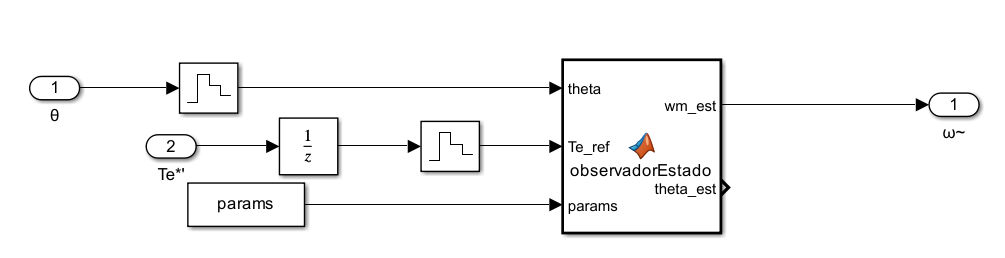
\includegraphics[width=0.60\linewidth]{imagenes/codificado_observador.png}
    \caption{Código implementado para el observador de estado de velocidad.}
    \label{fig:codificado_observador}
\end{figure}
\begin{lstlisting}[
caption={Código MATLAB Function del observador de estado de velocidad.},
label={lst:observador_velocidad}
]
function [wm_est, theta_est] = observadorEstado(theta, Te_ref, params)
% Observador discreto de velocidad y posición
% Implementación equivalente al modelo en bloques con integradores Tustin.
%
% Entradas:
%   theta   : posición medida [rad]
%   Te_ref  : torque electromagnético de referencia [N.m]
%   params  : estructura de parámetros del controlador
%
% Salidas:
%   wm_est    : velocidad estimada [rad/s]
%   theta_est : posición estimada [rad]

% =========================
% Lectura de parámetros
% =========================
Ts = params.Ts;
J_eq = params.J_eq;

K_e_i_m_int    = params.K_e_i_m_int;
K_e_w_m_int    = params.K_e_w_m_int;
K_e_tita_m_int = params.K_e_tita_m_int;

% =========================
% Estados persistentes
% =========================
persistent theta_est_k wm_est_k
persistent e_prev e_int_prev
persistent dw_prev dtheta_prev

if isempty(theta_est_k)

    theta_est_k = 0;
    wm_est_k    = 0;

    e_prev      = 0;
    e_int_prev  = 0;

    dw_prev     = 0;
    dtheta_prev = 0;
end

% =========================
% Error de posición
% =========================
e = theta - theta_est_k;

% =========================
% Integrador Tustin del error
% Bloque: Integrador Tustin2
% =========================
e_int = e_int_prev + (Ts/2)*(e + e_prev);

% =========================
% Dinámica de velocidad estimada
% =========================
dw = (1/J_eq)*Te_ref ...
   + K_e_i_m_int*e_int ...
   + K_e_w_m_int*e;

% =========================
% Integrador Tustin de velocidad
% Bloque: Integrador Tustin1
% =========================
wm_est_new = wm_est_k + (Ts/2)*(dw + dw_prev);

% =========================
% Dinámica de posición estimada
% =========================
dtheta = wm_est_new + K_e_tita_m_int*e;

% =========================
% Integrador Tustin de posición
% Bloque: Integrador Tustin3
% =========================
theta_est_new = theta_est_k + (Ts/2)*(dtheta + dtheta_prev);

% =========================
% Salidas
% =========================
wm_est    = wm_est_new;
theta_est = theta_est_new;

% =========================
% Actualización de estados
% =========================
theta_est_k = theta_est_new;
wm_est_k    = wm_est_new;

e_prev      = e;
e_int_prev  = e_int;

dw_prev     = dw;
dtheta_prev = dtheta;

end
\end{lstlisting}
\subsubsection{Modulador de torque}
El modulador de torque transforma la referencia de torque mecánico $T_m^{**}$ en una referencia de corriente de eje $q$, $i_{qs}^{r*}$. En este cálculo se incluyen las compensaciones de fricción viscosa y de torque gravitatorio, de manera que la corriente solicitada al motor contemple tanto la acción de control como los esfuerzos mecánicos propios de la carga. Además, la salida se limita según la corriente máxima admisible del accionamiento.
\begin{figure}[H]
    \centering
    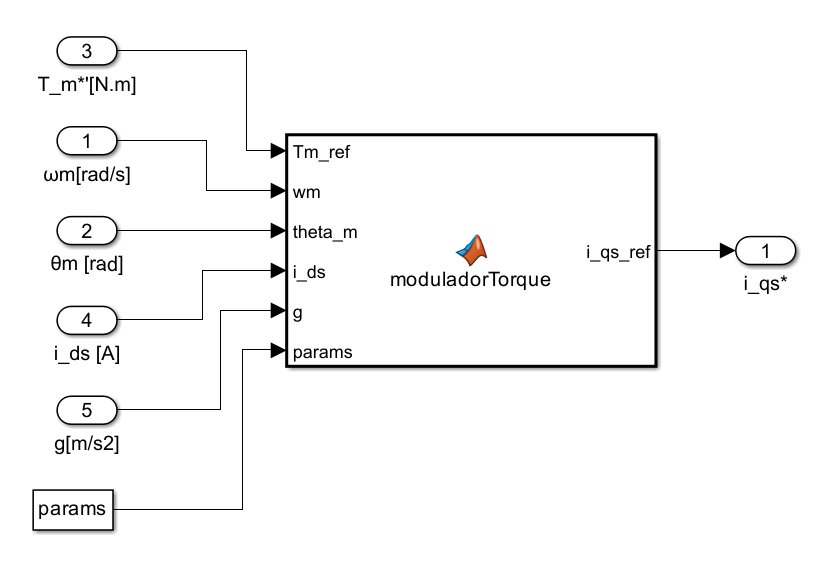
\includegraphics[width=0.60\linewidth]{imagenes/codificado_modTorque.png}
    \caption{Código implementado para el modulador de torque.}
    \label{fig:codificado_modTorque}
\end{figure}
\begin{lstlisting}[
caption={Código MATLAB Function del modulador de torque.},
label={lst:modulador_torque}
]
function i_qs_ref = moduladorTorque(Tm_ref, wm, theta_m, i_ds, g, params)
% Modulador de torque para PMSM.
%
% Calcula la referencia de corriente q:
%
%   i_qs_ref = T_eq / Kt_eq
%
% donde:
%   T_eq  = Tm_ref + b_eq*wm + torque_gravitatorio
%   Kt_eq = (3/2)*Pp*(lambda_m + (Ld - Lq)*i_ds)
%
% Entradas:
%   Tm_ref   : torque mecánico de referencia [N.m]
%   wm       : velocidad mecánica [rad/s]
%   theta_m  : posición mecánica [rad]
%   i_ds     : corriente eje d [A]
%   g        : gravedad [m/s^2]
%   params   : estructura de parámetros
%
% Salida:
%   i_qs_ref : referencia de corriente eje q [A]

% =========================
% Lectura de parámetros
% =========================
b_eq     = params.b_eq;
r        = params.r_red;
kl       = params.kl;
Ld       = params.Ld;
Lq       = params.Lq;
Pp       = params.Pp;
lambda_m = params.lambda_m;
Is_pico  = params.Is_pico;

% =========================
% Compensación viscosa
% =========================
T_visc = b_eq * wm;

% =========================
% Compensación gravitatoria
% =========================
theta_l = theta_m / r;
T_grav = (kl / r) * sin(theta_l) * g;

% =========================
% Torque equivalente requerido
% =========================
T_eq = Tm_ref + T_visc + T_grav;

% =========================
% Constante de torque equivalente
% =========================
Kt_eq = (3/2) * Pp * (lambda_m + (Ld - Lq) * i_ds);

% =========================
% Cálculo de corriente q de referencia
% =========================
i_qs_unsat = T_eq / Kt_eq;

% =========================
% Saturación entre -Is_pico e Is_pico
% =========================
if i_qs_unsat > Is_pico
    i_qs_ref = Is_pico;
elseif i_qs_unsat < -Is_pico
    i_qs_ref = -Is_pico;
else
    i_qs_ref = i_qs_unsat;
end

end
\end{lstlisting}

\subsubsection{Modulador de corriente}
El modulador de corriente implementa el lazo interno del controlador. Su función es comparar las corrientes de referencia con las corrientes medidas en los ejes $q$, $d$ y $0$, generando referencias de tensión proporcionales al error de cada eje. De esta forma se obtienen las señales $v_{qs}^{r*}$, $v_{ds}^{r*}$ y $v_{0s}^{*}$, que luego son corregidas por el bloque de desacople antes de aplicarse a la máquina.
\begin{figure}[H]
    \centering
    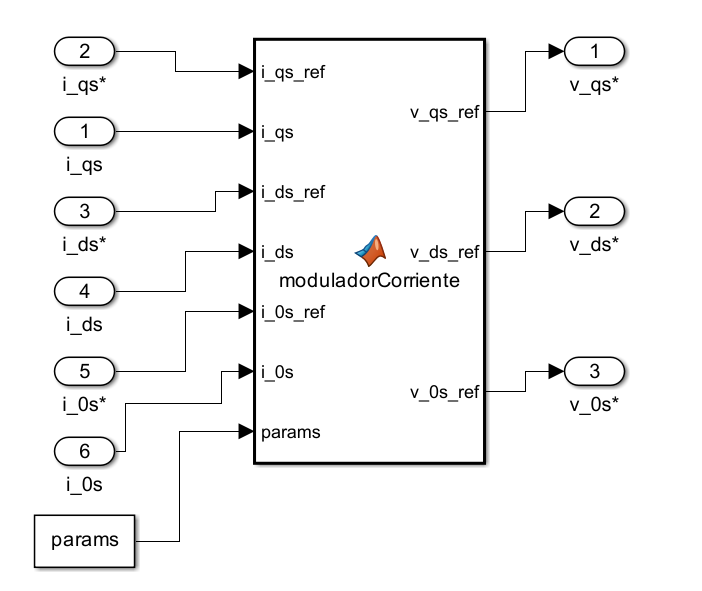
\includegraphics[width=0.60\linewidth]{imagenes/codificado_modCorr.png}
    \caption{Código implementado para el modulador de corriente.}
    \label{fig:codificado_modCorr}
\end{figure}
\begin{lstlisting}[
caption={Código MATLAB Function del modulador de corriente.},
label={lst:modulador_corriente}
]
function [v_qs_ref, v_ds_ref, v_0s_ref] = moduladorCorriente(i_qs_ref, i_qs, i_ds_ref, i_ds, i_0s_ref, i_0s, params)
% Modulador de corriente.
% Implementa control proporcional independiente en los ejes q, d y 0.
%
% Entradas:
%   i_qs_ref : referencia de corriente eje q [A]
%   i_qs     : corriente medida eje q [A]
%   i_ds_ref : referencia de corriente eje d [A]
%   i_ds     : corriente medida eje d [A]
%   i_0s_ref : referencia de corriente eje 0 [A]
%   i_0s     : corriente medida eje 0 [A]
%   params   : estructura de parámetros
%
% Salidas:
%   v_qs_ref : referencia de tensión eje q [V]
%   v_ds_ref : referencia de tensión eje d [V]
%   v_0s_ref : referencia de tensión eje 0 [V]

% =========================
% Lectura de parámetros
% =========================
K_pq = params.K_pq;
K_pd = params.K_pd;
K_p0 = params.K_p0;

% =========================
% Errores de corriente
% =========================
e_iq = i_qs_ref - i_qs;
e_id = i_ds_ref - i_ds;
e_i0 = i_0s_ref - i_0s;

% =========================
% Ley proporcional
% =========================
v_qs_ref = K_pq * e_iq;
v_ds_ref = K_pd * e_id;
v_0s_ref = K_p0 * e_i0;

end
\end{lstlisting}
\subsubsection{Desacoplamiento de realimentaciones físicas naturales}
El bloque de desacople agrega a las tensiones de control los términos físicos naturales presentes en el modelo eléctrico de la PMSM. En particular, incorpora las caídas resistivas de los devanados y los acoplamientos dependientes de la velocidad mecánica. Esto permite que las tensiones finales aplicadas al modelo no lineal reproduzcan la acción de control diseñada sobre el modelo desacoplado.
\begin{figure}[H]
    \centering
    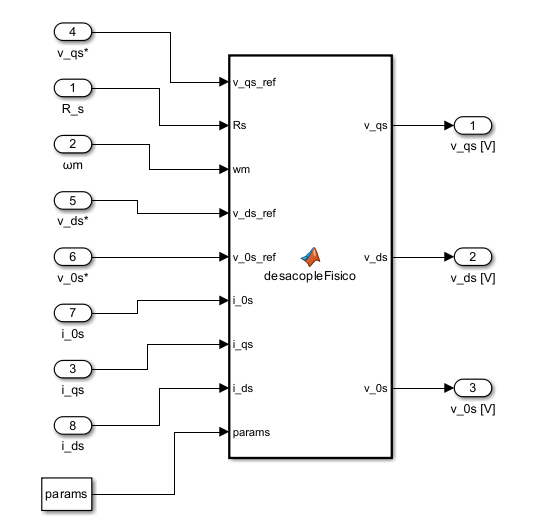
\includegraphics[width=0.60\linewidth]{imagenes/codificado_desacople.png}
    \caption{Código implementado para el desacople de realimentaciones físicas naturales.}
    \label{fig:codificado_desacople}
\end{figure}
\begin{lstlisting}[
caption={Código MATLAB Function del desacople de realimentaciones físicas naturales.},
label={lst:desacople_realimentaciones}
]
function [v_qs, v_ds, v_0s] = desacopleFisico(v_qs_ref, Rs, wm, v_ds_ref, v_0s_ref, i_0s, i_qs, i_ds, params)
% Desacople de realimentaciones físicas naturales de la PMSM.
%
% Entradas:
%   v_qs_ref : tensión q de control [V]
%   Rs       : resistencia estatórica actual [ohm]
%   wm       : velocidad mecánica [rad/s]
%   v_ds_ref : tensión d de control [V]
%   v_0s_ref : tensión 0 de control [V]
%   i_0s     : corriente eje 0 [A]
%   i_qs     : corriente eje q [A]
%   i_ds     : corriente eje d [A]
%   params   : estructura de parámetros
%
% Salidas:
%   v_qs : tensión q desacoplada [V]
%   v_ds : tensión d desacoplada [V]
%   v_0s : tensión 0 desacoplada [V]

% =========================
% Lectura de parámetros
% =========================
lambda_m = params.lambda_m;
Ld       = params.Ld;
Lq       = params.Lq;
Pp       = params.Pp;

% =========================
% Términos de desacople eje q
% =========================
lambda_eq = lambda_m + Ld*i_ds;

v_qs_ff = wm * Pp * lambda_eq;

% =========================
% Términos de desacople eje d
% =========================
v_ds_ff = -wm * Pp * Lq * i_qs;

% =========================
% Caídas resistivas
% =========================
v_Rq = Rs * i_qs;
v_Rd = Rs * i_ds;
v_R0 = Rs * i_0s;

% =========================
% Tensiones finales
% =========================
v_qs = v_qs_ref + v_Rq + v_qs_ff;
v_ds = v_ds_ref + v_Rd + v_ds_ff;
v_0s = v_0s_ref + v_R0;

end
\end{lstlisting}
\subsubsection{Transformación directa e inversa de Park}
Las transformaciones de Park permiten vincular el sistema trifásico físico con el sistema rotórico $qd0$ utilizado por el controlador. La transformación directa convierte las corrientes medidas de fase en corrientes $i_{qs}^r$, $i_{ds}^r$ e $i_{0s}$, utilizadas por el modulador de corriente. La transformación inversa realiza el proceso opuesto para las tensiones, obteniendo las consignas trifásicas que alimentan al inversor.
\begin{figure}[H]
    \centering
    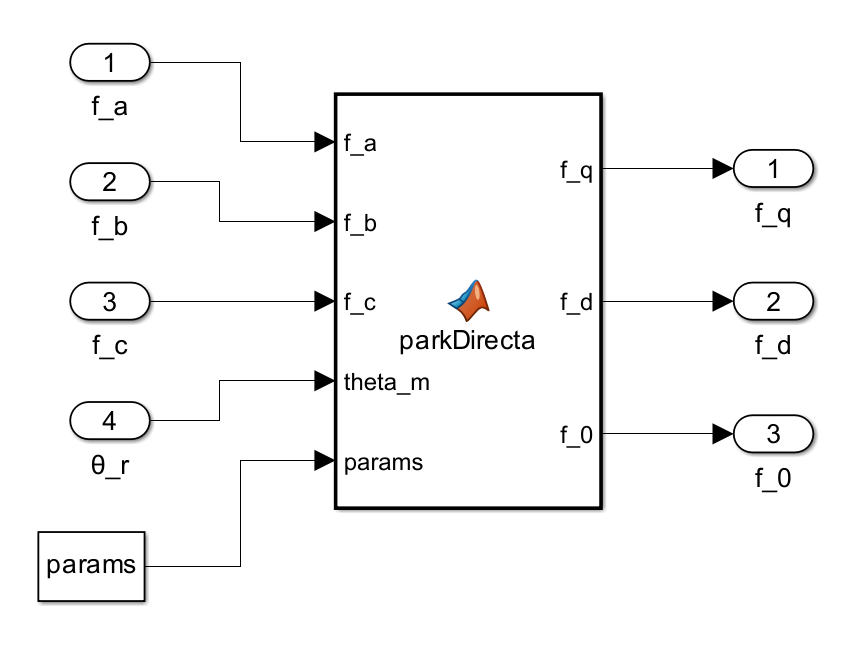
\includegraphics[width=0.60\linewidth]{imagenes/codificado_parkDir.png}
    \caption{Código implementado para la transformación directa de Park.}
    \label{fig:codificado_parkDir}
\end{figure}
\begin{figure}[H]
    \centering
    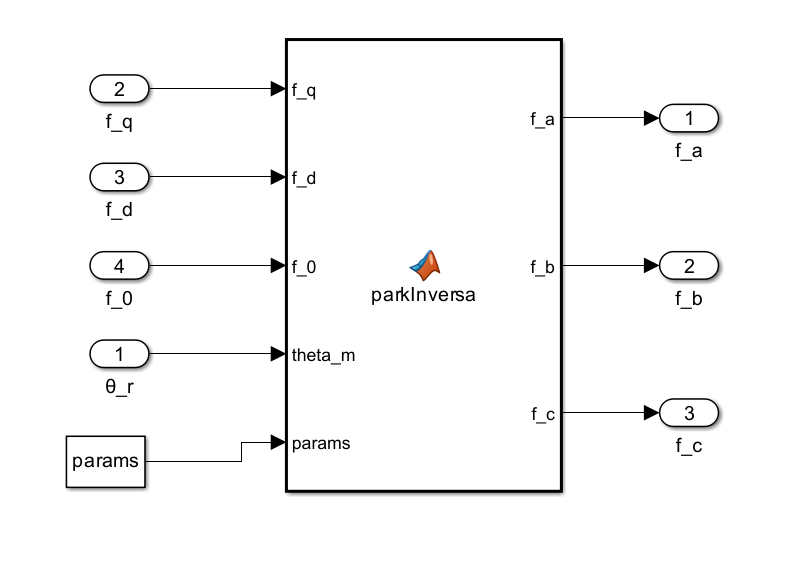
\includegraphics[width=0.60\linewidth]{imagenes/codificado_parkInv.png}
    \caption{Código implementado para la transformación inversa de Park.}
    \label{fig:codificado_parkInv}
\end{figure}
\begin{lstlisting}[
caption={Código MATLAB Function de la transformación directa de Park.},
label={lst:park_directa}
]
function [f_q, f_d, f_0] = parkDirecta(f_a, f_b, f_c, theta_m, params)

Pp = params.Pp;
theta = Pp * theta_m;

theta_a = theta;
theta_b = theta - 2*pi/3;
theta_c = theta + 2*pi/3;

c_a = cos(theta_a);
c_b = cos(theta_b);
c_c = cos(theta_c);

s_a = sin(theta_a);
s_b = sin(theta_b);
s_c = sin(theta_c);

f_q = (2/3)*(f_a*c_a + f_b*c_b + f_c*c_c);

f_d = (2/3)*(f_a*s_a + f_b*s_b + f_c*s_c);

f_0 = (1/3)*(f_a + f_b + f_c);

end
\end{lstlisting}
\begin{lstlisting}[
caption={Código MATLAB Function de la transformación inversa de Park.},
label={lst:park_inversa}
]
function [f_a, f_b, f_c] = parkInversa(f_q, f_d, f_0, theta_m, params)

Pp = params.Pp;
theta = Pp * theta_m;

theta_a = theta;
theta_b = theta - 2*pi/3;
theta_c = theta + 2*pi/3;

f_a = f_q*cos(theta_a) + f_d*sin(theta_a) + f_0;
f_b = f_q*cos(theta_b) + f_d*sin(theta_b) + f_0;
f_c = f_q*cos(theta_c) + f_d*sin(theta_c) + f_0;

end
\end{lstlisting}
\subsection{Comparación con el modelo continuo}
\begin{figure}[H]
    \centering
    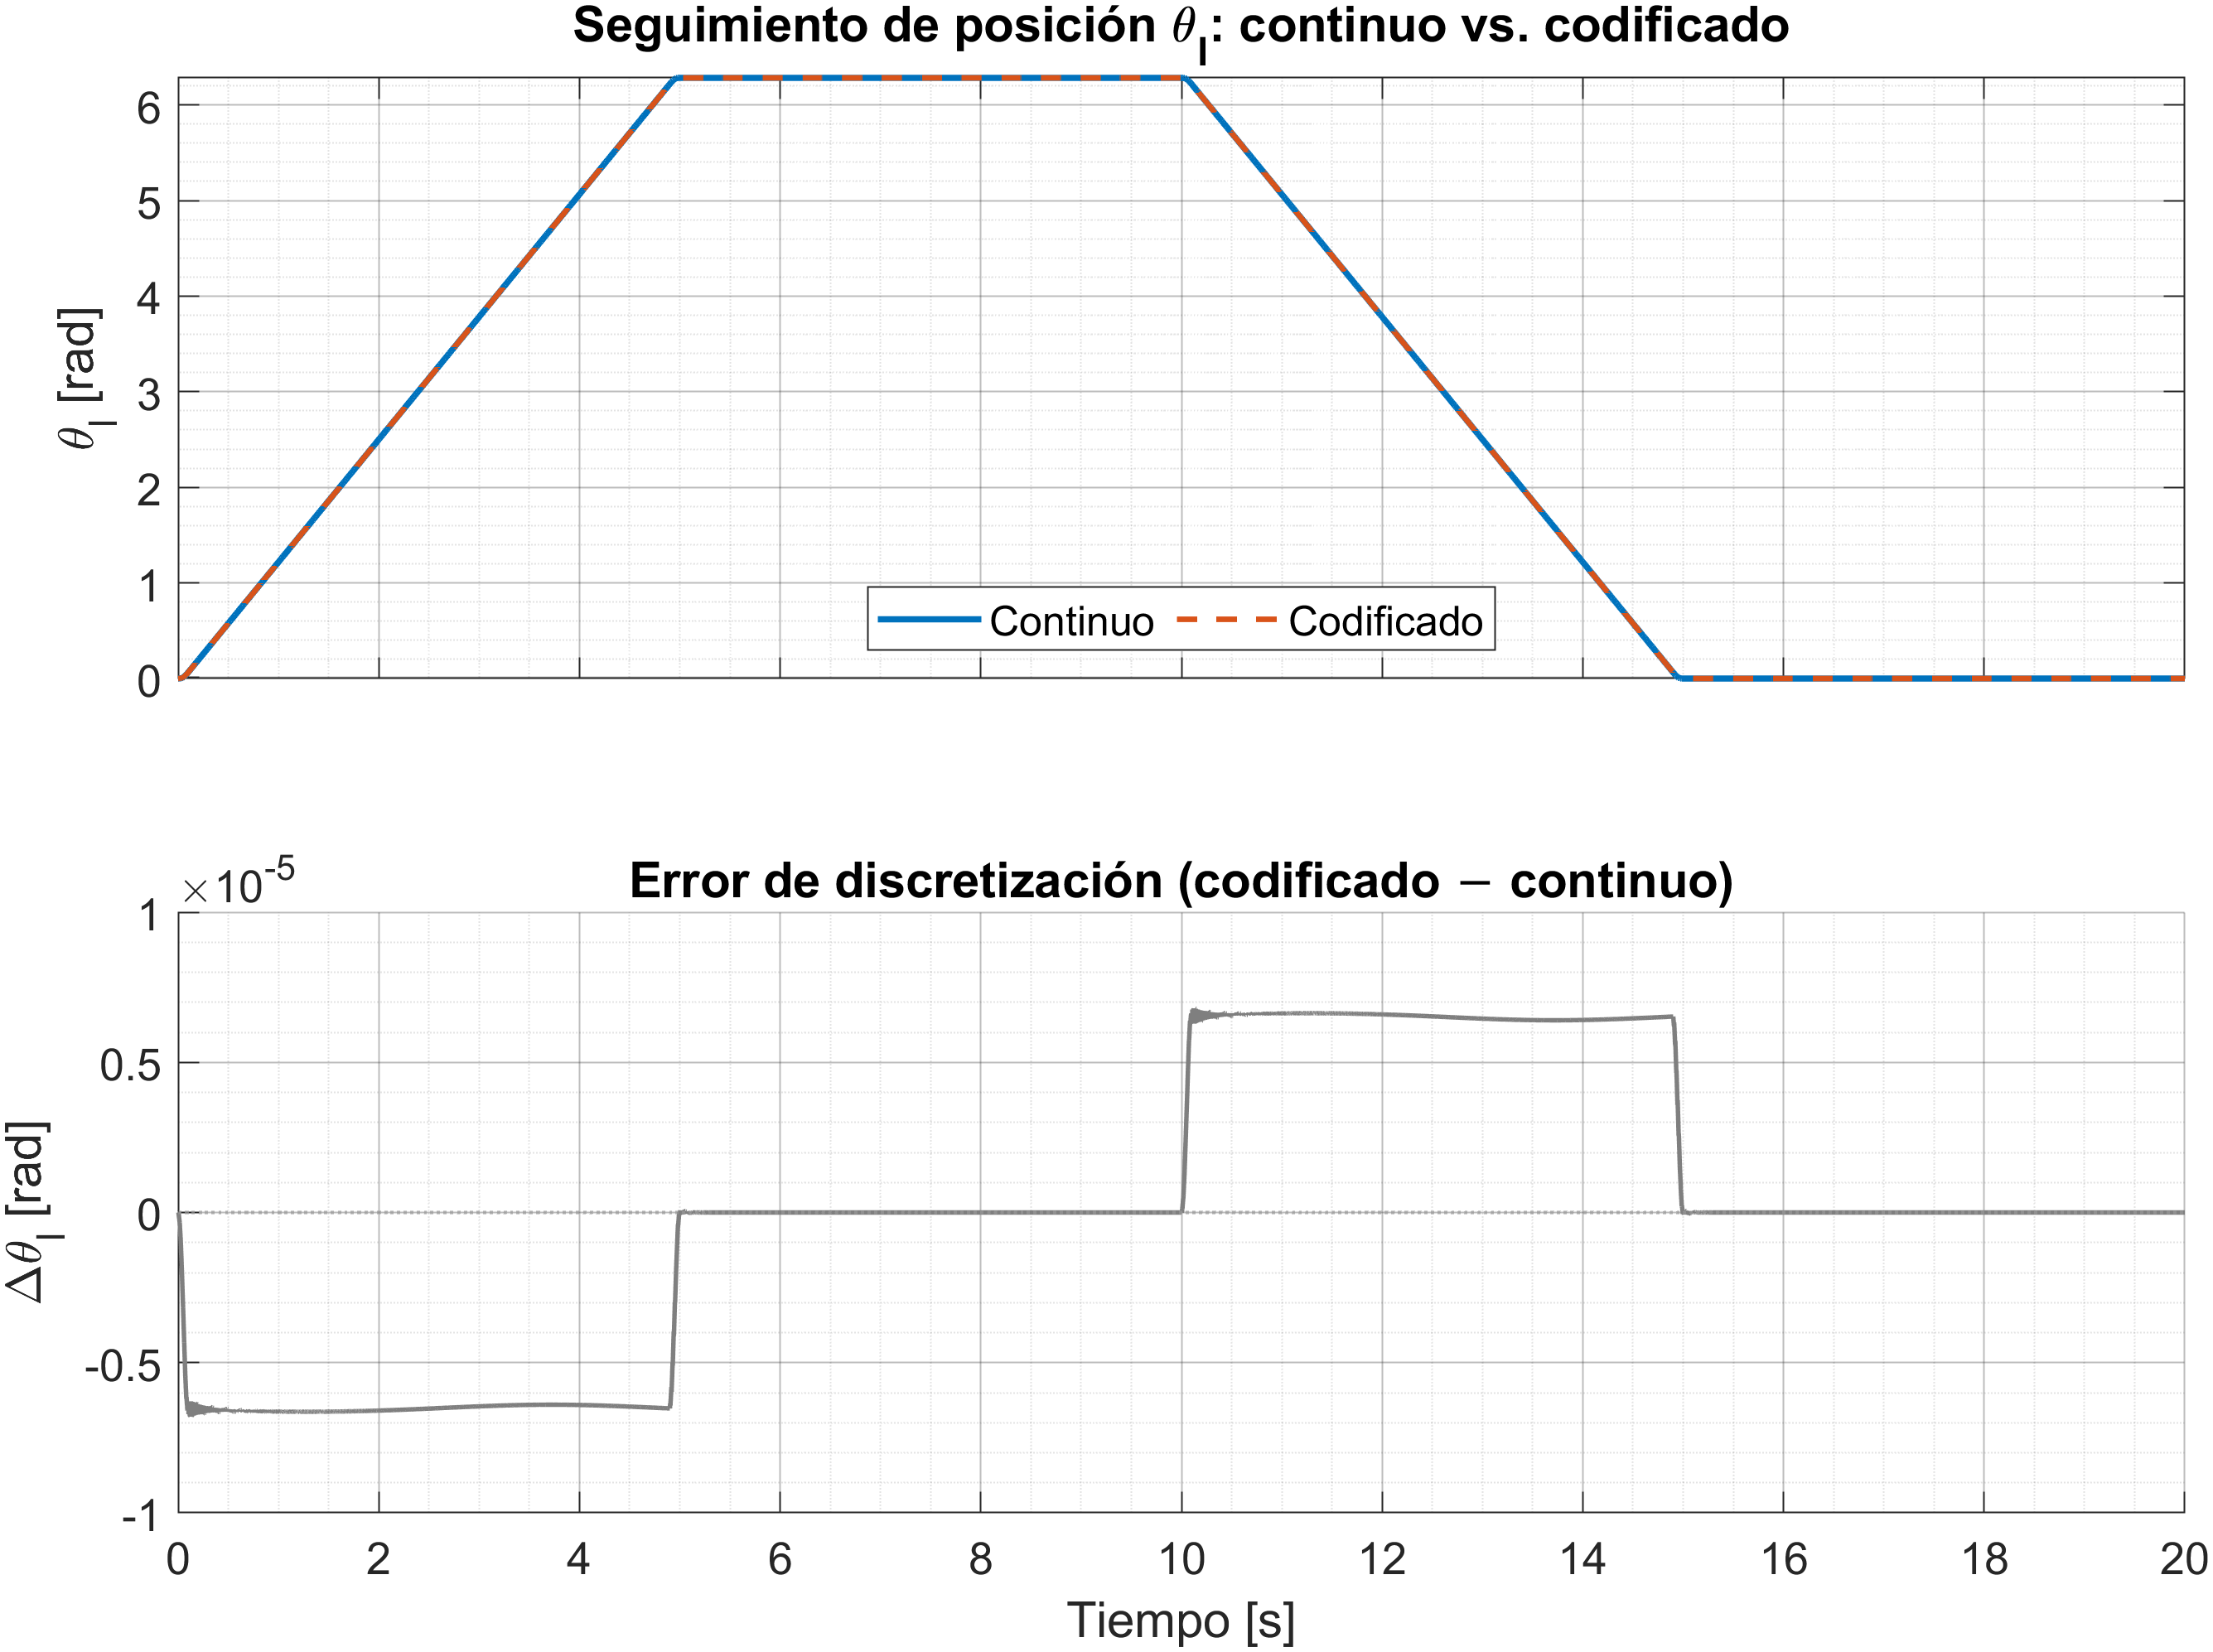
\includegraphics[width=0.60\linewidth]{imagenes/comp_codcont_pos.png}
    \caption{Comparación de seguimiento de consigna de posición del modelo continuo vs el codificado discreto.}
    \label{fig:comp_codcont_pos}
\end{figure}
\begin{figure}[H]
    \centering
    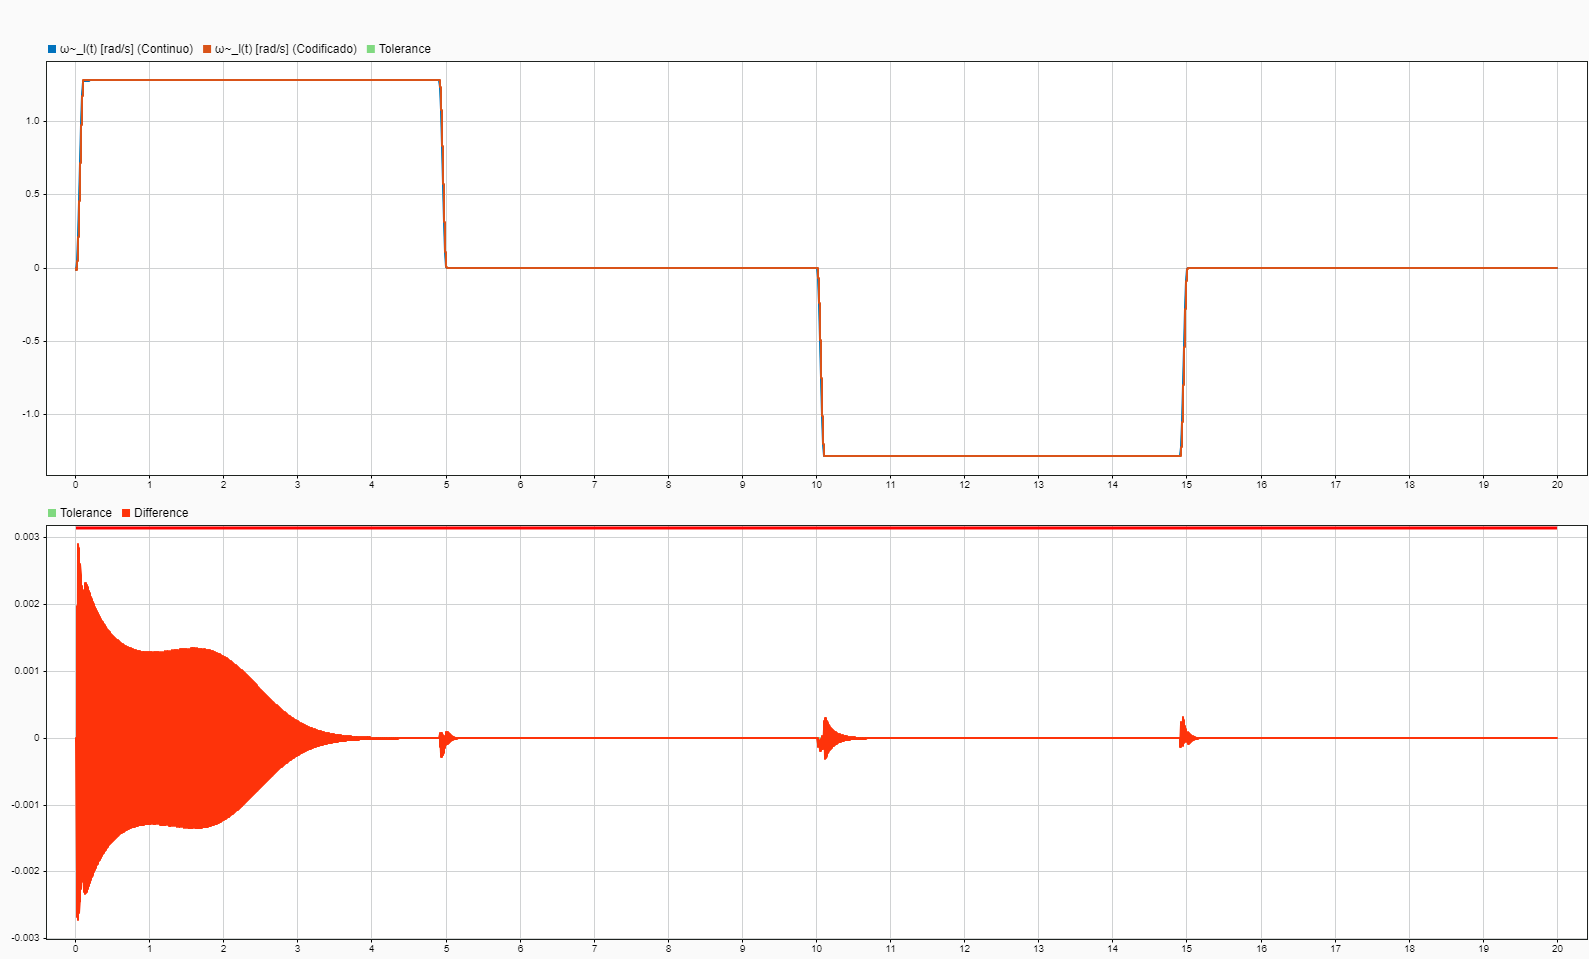
\includegraphics[width=0.60\linewidth]{imagenes/comp_codcont_vel.png}
    \caption{Comparación de seguimiento de consigna de velocidad del modelo continuo vs el codificado discreto.}
    \label{fig:comp_codcont_vel}
\end{figure}
Puede verse cómo el modelo codificado cumple con creces las expectativas de seguimiento de consigna, con un error despreciable de origen numérico proveniente de la discretización.
\section{Conclusiones}

El presente trabajo abordó el modelado, análisis y diseño de un sistema de control de posición y movimiento para un accionamiento eléctrico basado en un motor sincrónico de imanes permanentes (PMSM) acoplado, mediante un reductor planetario de relación $r=120{:}1$, a una carga mecánica del tipo péndulo rígido de un grado de libertad. A partir del modelo no lineal completo de seis estados en coordenadas rotóricas $qd0$, se derivó un modelo LTI equivalente aumentado de cuatro estados mediante una linealización por retroalimentación NL de estado, empleando una ley mínima sobre $v_{ds}^{r}$ y una ley complementaria sobre $v_{qs}^{r}$ que cancelan en forma exacta los acoplamientos electromagnéticos cruzados. La simulación dinámica comparativa frente a la secuencia de pulsos de tensión y torque de carga prevista en la guía verificó la equivalencia entre el modelo no lineal y el LTI aumentado, así como el carácter transitorio de la dinámica residual de $i_{ds}^{r}$ ante condiciones iniciales no nulas, con constante de tiempo $\tau_d = L_d/R_s \approx 6{,}24$~ms.

Los análisis estructurales mostraron que $i_{ds}^{r}$ es simultáneamente no controlable desde $v_{qs}^{r}$ y no observable desde $\theta_m$, lo que justifica formalmente la cancelación polo-cero detectada en las funciones de transferencia y permitió diseñar un observador reducido de la parte mecánica a partir únicamente del sensor de posición, sin pérdida de información estructural relevante. Sobre esta base se diseñó un controlador en cascada compuesto por un modulador de torque con desacoplamiento completo y torque precalculado gravitatorio y viscoso, lazos proporcionales de corriente con polo en $-5000$ rad/s y un controlador PID externo sintonizado por el método de sintonía serie con $\zeta = 0{,}75$ y $\omega_n = 800$~rad/s. El observador mecánico se ubicó originalmente con polos dobles en $-3200$~rad/s y, posteriormente, debió aumentarse con acción integral para eliminar el error estacionario de estimación frente a perturbaciones constantes de carga, ubicando tres polos reales iguales en $-3200$~rad/s.

La verificación de desempeño puso de manifiesto varias limitaciones operativas del sistema diseñado. En primer lugar, ante consignas de posición con discontinuidades en aceleración o velocidad, las corrientes de fase superan las especificaciones nominales, por lo que se incorporó un generador de trayectorias con perfil trapezoidal de aceleración (curva en S) que respeta las restricciones del inversor y del motor. En segundo lugar, bajo operación cíclica con $T_{amb}^\circ=25\,^\circ$C y $T_{ld}=5$~Nm, la temperatura del bobinado supera el límite admisible de $115\,^\circ$C a los $225{,}9$~s ($\approx 15$ ciclos completos), indicando que el accionamiento no satisface el requerimiento térmico de operación continua repetitiva bajo esas condiciones. En tercer lugar, el modelado realista de sensores e inversor como filtros pasa bajos en espacio de estados evidenció que las dinámicas especificadas en la guía no son lo suficientemente rápidas: fue necesario escalar los polos de los sensores en un factor $N=3$ y duplicar el ancho de banda del inversor hasta $\omega_n^{\prime}=12000$~rad/s para no degradar el desempeño del controlador.

Finalmente, se completó la transición a tiempo discreto mediante la regla de Tustin con $T_s \leq 1{,}25\times 10^{-4}$~s, discretizando los integradores del PID externo y del observador y modelando la frontera digital-analógica con retenedores de orden cero. La codificación modular del controlador mediante un conjunto de \textit{MATLAB Functions} independientes permitió validar su equivalencia con el diseño en bloques, sentando las bases para una eventual implementación física sobre microcontrolador o DSP.

Como líneas de mejora se identifican: la incorporación de una estrategia de campo orientado con maximización del torque por amperio (MTPA), la implementación de un esquema de disipación térmica activa o la reformulación del ciclo de trabajo para garantizar la operación continua admisible, la evaluación cuantitativa de la robustez del controlador ante la variación máxima de los parámetros de carga $J_l$ y $b_l$, y la validación experimental del controlador discretizado sobre una plataforma física.

\bibliographystyle{ieeetr}
\bibliography{references}





%%%%%%%% APPENDIX %%%%%%%%



\appendices
\section{Generador de Trayectorias con perfil de aceleración trapezoidal (curva en S)}
\subsection{Descripción General}
Para el control de posición del motor sincrónico de imanes permanentes (PMSM), se incorporó un \textbf{Generador de Trayectorias} en el esquema de control. Este bloque tiene como objetivo principal suavizar las transiciones entre los distintos puntos de consigna espaciales, generando referencias continuas y derivables de posición ($\theta_{ref}$), velocidad ($\omega_{ref}$) y aceleración ($\alpha_{ref}$) en función del tiempo. 

El algoritmo implementa un perfil de velocidad trapezoidal suavizado, comúnmente denominado \textit{curva en S de 7 tramos}. Esta técnica permite limitar el \textit{jerk} (la derivada temporal de la aceleración), lo cual es fundamental para evitar excitaciones bruscas en la mecánica del rotor y la carga, prevenir picos de corriente excesivos en las fases del estator y mitigar la saturación prematura de los actuadores y lazos de control.

\subsection{Dinámica del Perfil de 7 Tramos}
Para trasladar el rotor desde una posición inicial a una final en un intervalo de tiempo dado, el algoritmo divide internamente el movimiento en tres fases principales, que a su vez componen los 7 subtramos característicos de la curva en S:
\begin{enumerate}
    \item \textbf{Fase de Aceleración:} El \textit{jerk} toma un valor constante positivo haciendo que la aceleración suba linealmente hasta su límite. Luego, la aceleración se mantiene constante, y finalmente el \textit{jerk} se vuelve negativo para llevar la aceleración suavemente a cero conforme se alcanza la velocidad máxima de crucero.
    \item \textbf{Fase de Velocidad Constante:} La aceleración y el \textit{jerk} son nulos. El sistema se desplaza a la velocidad máxima calculada para el tramo hasta que es necesario comenzar a frenar.
    \item \textbf{Fase de Desaceleración (Frenado):} De forma simétrica a la primera fase, se aplican perfiles de \textit{jerk} controlados para generar una aceleración negativa suave, frenando el motor hasta alcanzar exactamente la posición de destino con velocidad y aceleración finales nulas.
\end{enumerate}

\subsection{Parámetros y Variables de Configuración}
El bloque procesa los siguientes parámetros para generar las señales en tiempo de simulación:
\begin{itemize}
    \item $t$: Tiempo actual de simulación [s].
    \item \texttt{consigna\_posicion}: Matriz de $N \times 2$ donde la primera columna contiene los instantes de tiempo (nodos temporales) y la segunda indica las posiciones angulares objetivo para cada nodo.
    \item $t_{r1}$ (\texttt{t\_rampa\_vel}): Tiempo total asignado a la fase completa de aceleración (o desaceleración).
    \item $t_{r2}$ (\texttt{t\_rampa\_acel}): Fracción de tiempo dedicada exclusivamente al incremento o decremento lineal de la aceleración (fase de \textit{jerk} distinto de cero).
\end{itemize}

A nivel algorítmico y para optimizar la carga computacional en cada paso de integración de la simulación, el sistema precalcula las distancias relativas entre nodos ($\Delta q$), las duraciones de los tramos ($\Delta t$), la velocidad máxima requerida ($h_1$) y la aceleración máxima ($h_2$) una única vez durante el primer ciclo de ejecución, operando luego mediante la evaluación temporal sobre estos límites preestablecidos.
\label{anexo:gen_trayectorias}
\end{document}
